%%%%%%%%%%%%%%%%%%%%%%%%%%%%% Thesis.tex %%%%%%%%%%%%%%%%%%%%%%%%%%%%%%%
%                                                                      %
%  ---------- Master of Science Dissertation template ----------       %
%                                                                      %
%  Template for the Master Thesis according to the regulations         %
%  published by the Academic Board (Direcção Académica) at IST.        %
%                                                                      %
%  For up-to-date guide, please refer to the official website          %
%
% https://tecnico.ulisboa.pt/pt/ensino/estudar-no-tecnico/informacoes-academicas/dissertacao-de-mestrado/
%                                                                      %
%       Andre C. Marta                                                 %
%       Area Cientifica de Mecanica Aplicada e Aeroespacial            %
%       Departamento de Engenharia Mecanica                            %
%       Instituto Superior Tecnico                                     %
%       Av. Rovisco Pais                                               %
%       1049-001 Lisboa                                                %
%       Portugal                                                       %
%       Tel: +351 21 841 9469                                          %
%                        3469 (extension)                              %
%       Email: andre.marta@tecnico.ulisboa.pt                          %
%                                                                      %
%  Created:       Jan 20, 2011                                         %
%  Last Modified: Mar  4, 2024                                         %
%                                                                      %
%%%%%%%%%%%%%%%%%%%%%%%%%%%%%%%%%%%%%%%%%%%%%%%%%%%%%%%%%%%%%%%%%%%%%%%%
%  Revision history                                                    %
%  v1 - 2011/01/24 - original template                                 %
%  v2 - 2012/10/30 - new IST image and glossary support                %
%  v3 - 2013/12/10 - update according to 2012/13 official guide        %
%  v4 - 2014/02/28 - new default for bibliography style                %
%  v5 - 2014/05/07 - update according to 2013/14 official guide        %
%  v6 - 2015/07/02 - cover page format fixed,                          %
%                    contents page numbering fixed,                    %
%                    better language support,                          %
%                    enhanced examples of tables,                      %
%                    new option for appendix page numbering format,    %
%                    custom bibliography style                         %
%  v7 - 2018/02/19 - multiple citations compressed                     %
%  v8 - 2019/05/13 - added examples (pseudo-code)                      %
%  v9 - 2020/03/03 - added French language support                     %
%                    indented first paragraphs                         %
%  v10- 2021/01/29 - place caption above table                         %
%  v11- 2022/06/29 - included Declaration of original work             %
%  v12- 2024/02/26 - new glossaries and subfig packages                %
%%%%%%%%%%%%%%%%%%%%%%%%%%%%%%%%%%%%%%%%%%%%%%%%%%%%%%%%%%%%%%%%%%%%%%%%
%                                                                      %
% To generate the PDF file, type "make" at the terminal prompt.        %
%                                                                      %
% This IST template LaTeX package was created by the author            %
% and it can be downloaded from:                                       %
%    https://fenix.tecnico.ulisboa.pt/homepage/ist31052/               %
% or https://mdo.tecnico.ulisboa.pt/templates/                         %
%                                                                      %
% The external packages can be downloaded from                         %
% the Comprehensive TeX Archive Network at http://www.ctan.org/        %
%                                                                      %
% List of LaTex symbols:                                               %
% http://www.ctan.org/tex-archive/info/symbols/comprehensive/          %
%                                                                      %
% Help with LaTex can be found at                                      %
% http://en.wikibooks.org/wiki/LaTeX                                   %
%%%%%%%%%%%%%%%%%%%%%%%%%%%%%%%%%%%%%%%%%%%%%%%%%%%%%%%%%%%%%%%%%%%%%%%%

%%%%%%%%%%%%%%%%%%%%%%%%%%%%%%%%%%%%%%%%%%%%%%%%%%%%%%%%%%%%%%%%%%%%%%%%
%     Preamble                                                         %
%%%%%%%%%%%%%%%%%%%%%%%%%%%%%%%%%%%%%%%%%%%%%%%%%%%%%%%%%%%%%%%%%%%%%%%%

% Generate nomencalture and glossary
\immediate\write18{makeindex \jobname.nlo -s nomencl.ist -o \jobname.nls}

% ----------------------------------------------------------------------
%  Set the document class
% ----------------------------------------------------------------------
\documentclass[10pt,a4paper,twoside]{report}

% ----------------------------------------------------------------------
% Define external packages, language, margins, fonts and new commands
% ----------------------------------------------------------------------
%%%%%%%%%%%%%%%%%%%%%%%%%%%%%%%%%%%%%%%%%%%%%%%%%%%%%%%%%%%%%%%%%%%%%%%%
%                                                                      %
%     File: Thesis_Preamble.tex                                        %
%     Tex Master: Thesis.tex                                           %
%                                                                      %
%     Author: Andre C. Marta                                           %
%     Last modified :  4 Mar 2024                                      %
%                                                                      %
%%%%%%%%%%%%%%%%%%%%%%%%%%%%%%%%%%%%%%%%%%%%%%%%%%%%%%%%%%%%%%%%%%%%%%%%

% 'natbib' package
%
% Flexible bibliography support.
% https://www.ctan.org/pkg/natbib
%
% > produce author-year style citations
%
% \citet  and \citep  for textual and parenthetical citations, respectively
% \citet* and \citep* that print the full author list, and not just the abbreviated one
% \citealt is the same as \citet but without parentheses. Similarly, \citealp is \citep without parentheses
% \citeauthor
% \citeyear
% \citeyearpar
%
%% natbib options can be provided when package is loaded \usepackage[options]{natbib}
%%
%% Following options are valid:
%%
%%   round  -  round parentheses are used (default)
%%   square -  square brackets are used   [option]
%%   curly  -  curly braces are used      {option}
%%   angle  -  angle brackets are used    <option>
%%   semicolon  -  multiple citations separated by semi-colon (default)
%%   colon  - same as semicolon, an earlier confusion
%%   comma  -  separated by comma
%%   authoryear - for author–year citations (default)
%%   numbers-  selects numerical citations
%%   super  -  numerical citations as superscripts, as in Nature
%%   sort   -  sorts multiple citations according to order in ref. list
%%   sort&compress   -  like sort, but also compresses numerical citations
%%   compress - compresses without sorting
%%
% ******************************* SELECT *******************************
%\usepackage{natbib}          % <<<<< References in alphabetical list Correia, Silva, ...
\usepackage[numbers,sort&compress]{natbib} % <<<<< References in numbered list [1],[2],...
% ******************************* SELECT *******************************


% 'notoccite' package
%
% Prevent trouble from citations in table of contents, etc.
% http://ctan.org/pkg/notoccite
%
% > If you have \cite commands in \section-like commands, or in \caption,
%   the citation will also appear in the table of contents, or list of whatever.
%   If you are also using an unsrt-like bibliography style, these citations will
%   come at the very start of the bibliography, which is confusing. This pack­age
%   suppresses the effect.
%
\usepackage{notoccite}


% ----------------------------------------------------------------------
% Define document language.
% ----------------------------------------------------------------------

% 'inputenc' package
%
% Accept different input encodings.
% https://www.ctan.org/pkg/inputenc
%
% > allows typing non-english text in LaTeX sources.
%
% ******************************* SELECT *******************************
%\usepackage[latin1]{inputenc} % <<<<< Windows
\usepackage[utf8]{inputenc}   % <<<<< Linux
% ******************************* SELECT *******************************

% 'babel' package
%
% Multilingual support for Plain TeX or LaTeX.
% https://www.ctan.org/pkg/babel
%
% > sets the variable names according to the language selected
%
% ******************************* SELECT *******************************
%\usepackage[portuguese]{babel} % <<<<< Portuguese
\usepackage[english]{babel} % <<<<< English
%\usepackage[francais]{babel} % <<<<< French (requires package texlive-lang-french)
% ******************************* SELECT *******************************

% 'nomencl' package
%
% Produce lists of symbols as in nomenclature.
% https://www.ctan.org/pkg/nomencl
%
% The nomencl package makes use of the MakeIndex program
% in order to produce the nomenclature list.
%
% Nomenclature
% 1) On running the file through LATEX, the command \makenomenclature
%    in the preamble instructs it to create/open the nomenclature file
%    <jobname>.nlo corresponding to the LATEX file <jobname>.tex and
%    writes the information from the \nomenclature commands to this file.
% 2) The next step is to invoke MakeIndex in order to produce the
%    <jobname>.nls file. This can be achieved by making use of the
%    command: makeindex <jobname>.nlo -s nomencl.ist -o <jobname>.nls
% 3) The last step is to invoke LATEX on the <jobname>.tex file once
%    more. There, the \printnomenclature in the document will input the
%    <jobname>.nls file and process it according to the given options.
%
% Nomenclature (produces *.nlo *.nls files)
\usepackage{nomencl}
\makenomenclature
%
% Group variables according to their symbol type
% (see <prefix> in Thesis_Nomenclature.tex)
%
\RequirePackage{ifthen} 
\ifthenelse{\equal{\languagename}{english}}%
    { % English
    \renewcommand{\nomgroup}[1]{%
      \ifthenelse{\equal{#1}{R}}{%
        \item[\textbf{Roman symbols}]}{%
        \ifthenelse{\equal{#1}{G}}{%
          \item[\textbf{Greek symbols}]}{%
          \ifthenelse{\equal{#1}{S}}{%
            \item[\textbf{Subscripts}]}{%
            \ifthenelse{\equal{#1}{T}}{%
              \item[\textbf{Superscripts}]}{}}}}}%
    }{%
    \ifthenelse{\equal{\languagename}{french}}%
    { % French
    \renewcommand{\nomgroup}[1]{%
      \ifthenelse{\equal{#1}{R}}{%
        \item[\textbf{Symbole romains}]}{%
        \ifthenelse{\equal{#1}{G}}{%
          \item[\textbf{Symboles grecs}]}{%
          \ifthenelse{\equal{#1}{S}}{%
            \item[\textbf{Indices}]}{% lettre inférieure
            \ifthenelse{\equal{#1}{T}}{%
              \item[\textbf{Exposants}]}{}}}}}% lettre supérieure
    }{ % Portuguese
    \renewcommand{\nomgroup}[1]{%
      \ifthenelse{\equal{#1}{R}}{%
        \item[\textbf{Simbolos romanos}]}{%
        \ifthenelse{\equal{#1}{G}}{%
          \item[\textbf{Simbolos gregos}]}{%
          \ifthenelse{\equal{#1}{S}}{%
            \item[\textbf{Subscritos}]}{%
            \ifthenelse{\equal{#1}{T}}{%
              \item[\textbf{Sobrescritos}]}{}}}}}%
    }}%


% 'hyperref' package
%
% Extensive support for hypertext in LaTeX.
% https://www.ctan.org/pkg/hyperref
%
% > Extends the functionality of all the LATEX cross-referencing
%   commands (including the table of contents, bibliographies etc) to
%   produce \special commands which a driver can turn into hypertext
%   links; Also provides new commands to allow the user to write adhoc
%   hypertext links, including those to external documents and URLs.
%
\usepackage[pdftex]{hyperref}  % enhance documents that are to be
% output as HTML and PDF
\hypersetup{colorlinks=true,   % color text of links and anchors,
% eliminates borders around links
linkcolor=gray,    % color for normal internal links
%            linkcolor=black,  % color for normal internal links
anchorcolor=black,% color for anchor text
citecolor=cyan,  % color for bibliographical citations
%            citecolor=black,  % color for bibliographical citations
%           filecolor=magenta,% color for URLs which open local files
filecolor=black,  % color for URLs which open local files
%           menucolor=red,    % color for Acrobat menu items
menucolor=black,  % color for Acrobat menu items
urlcolor=cyan,    % color for linked URLs
%            urlcolor=black,   % color for linked URLs
% 	        bookmarks=true,         % create PDF bookmarks
bookmarksopen=false,    % don't expand bookmarks
bookmarksnumbered=true, % number bookmarks
pdftitle={Thesis},
pdfauthor={Andre C. Marta},
pdfsubject={Thesis Title},
pdfkeywords={Thesis Keywords},
pdfstartview=FitV,
pdfdisplaydoctitle=true}


% 'glossaries' package
%
% Create glossaries and lists of acronyms
% https://www.ctan.org/pkg/glossaries
%
% The glossaries package makes use of the MakeIndex program
% in order to produce the glossary list.
%
% The following options are used:
%   - acronym      : to produce the list of acronyms
%   - nonumberlist : to remove the page number
%   - nopostdot    : to remove the dot at the end of definition of term
%   - nogroupskip  : to remove the line spacing between groups
%
% Glossary (produces *.glo *.ist files)
%
\usepackage[acronym,nonumberlist,nopostdot,nogroupskip]{glossaries}
\setglossarystyle{long}
\renewcommand{\glsnamefont}[1]{\textbf{#1}} % acronym in bold face
\makenoidxglossaries


% List of LaTeX variable names: \abstractname, \appendixname, \bibname,
%   \chaptername, \contentsname, \listfigurename, \listtablename, ...)
% https://texfaq.org/FAQ-fixnam
%
% Changing the words babel uses (uncomment and redefine as necessary...)
%
\newcommand{\acknowledgments}{@undefined} % new LaTeX variable name
%
% > English
%
\addto\captionsenglish{\renewcommand{\acknowledgments}{Acknowledgments}}
%\addto\captionsenglish{\renewcommand{\contentsname}{Contents}}
%\addto\captionsenglish{\renewcommand{\listtablename}{List of Tables}}
%\addto\captionsenglish{\renewcommand{\listfigurename}{List of Figures}}
%\addto\captionsenglish{\renewcommand{\nomname}{Nomenclature}} % (List of Symbols)
%\addto\captionsenglish{\renewcommand{\glossaryname}{Glossary}}
\addto\captionsenglish{\renewcommand{\acronymname}{List of acronyms}} % Acronyms
%\addto\captionsenglish{\renewcommand{\bibname}{References}} % Bibliography
%\addto\captionsenglish{\renewcommand{\appendixname}{Appendix}}

% > French
%
\addto\captionsfrench{\renewcommand{\acknowledgments}{Remerciements}}
%\addto\captionsfrench{\renewcommand{\contentsname}{Table des matières}}
%\addto\captionsfrench{\renewcommand{\listtablename}{Liste des tableaux}}
\addto\captionsfrench{\renewcommand{\listfigurename}{Liste des figures}} % Table des figures
%\addto\captionsfrench{\renewcommand{\nomname}{Nomenclature}}
%\addto\captionsfrench{\renewcommand{\glossaryname}{Glossaire}}
%\addto\captionsfrench{\renewcommand{\acronymname}{Liste des acronymes}}
%\addto\captionsfrench{\renewcommand{\bibname}{Bibliographie}}
%\addto\captionsfrench{\renewcommand{\appendixname}{Annexe}}

% > Portuguese
%
\addto\captionsportuguese{\renewcommand{\acknowledgments}{Agradecimentos}}
%\addto\captionsportuguese{\renewcommand{\contentsname}{Conte\'{u}do}}
%\addto\captionsportuguese{\renewcommand{\listtablename}{Lista de Figuras}}
%\addto\captionsportuguese{\renewcommand{\listfigurename}{Lista de Tabelas}}
\addto\captionsportuguese{\renewcommand{\nomname}{Lista de S\'{i}mbolos}} % Nomenclatura
%\addto\captionsportuguese{\renewcommand{\glossaryname}{Gloss\'{a}rio}}
%\addto\captionsportuguese{\renewcommand{\acronymname}{Lista de Abrevia\c{c}\~{o}es}}
%\addto\captionsportuguese{\renewcommand{\bibname}{Refer\^{e}ncias}} % Bibliografia
%\addto\captionsportuguese{\renewcommand{\appendixname}{Anexo}} % Apendice


% ----------------------------------------------------------------------
% Define cover fields in both english and portuguese.
% ----------------------------------------------------------------------
%
\newcommand{\coverThesis}{@undefined} % new LaTeX variable name
\newcommand{\coverSupervisors}{@undefined} % new LaTeX variable name
\newcommand{\coverExaminationCommittee}{@undefined} % new LaTeX variable name
\newcommand{\coverChairperson}{@undefined} % new LaTeX variable name
\newcommand{\coverSupervisor}{@undefined} % new LaTeX variable name
\newcommand{\coverMemberCommittee}{@undefined} % new LaTeX variable name
% > English
\addto\captionsenglish{\renewcommand{\coverThesis}{Thesis to obtain the Master of Science Degree in}}
\addto\captionsenglish{\renewcommand{\coverSupervisors}{Supervisor(s)}}
\addto\captionsenglish{\renewcommand{\coverExaminationCommittee}{Examination Committee}}
\addto\captionsenglish{\renewcommand{\coverChairperson}{Chairperson}}
\addto\captionsenglish{\renewcommand{\coverSupervisor}{Supervisor}}
\addto\captionsenglish{\renewcommand{\coverMemberCommittee}{Member of the Committee}}
% > French
\addto\captionsfrench{\renewcommand{\coverThesis}{Th\`ese pour l'obtention du Maîtrise des Sciences en}}
\addto\captionsfrench{\renewcommand{\coverSupervisors}{Directeur(s) de th\`ese}}
\addto\captionsfrench{\renewcommand{\coverExaminationCommittee}{Jury}}
\addto\captionsfrench{\renewcommand{\coverChairperson}{Pr\'esident}}
\addto\captionsfrench{\renewcommand{\coverSupervisor}{Directeur de th\`ese}}
\addto\captionsfrench{\renewcommand{\coverMemberCommittee}{Rapporteur}}
% > Portuguese
\addto\captionsportuguese{\renewcommand{\coverThesis}{Disserta\c{c}\~{a}o para obten\c{c}\~{a}o do Grau de Mestre em}}
\addto\captionsportuguese{\renewcommand{\coverSupervisors}{Orientador(es)}}
\addto\captionsportuguese{\renewcommand{\coverExaminationCommittee}{J\'{u}ri}}
\addto\captionsportuguese{\renewcommand{\coverChairperson}{Presidente}}
\addto\captionsportuguese{\renewcommand{\coverSupervisor}{Orientador}}
\addto\captionsportuguese{\renewcommand{\coverMemberCommittee}{Vogal}}


% ----------------------------------------------------------------------
% Define Declaration of original work in both english and portuguese.
% ----------------------------------------------------------------------
%
\newcommand{\declarationTitle}{@undefined} % new LaTeX variable name
\newcommand{\declarationText}{@undefined}  % new LaTeX variable name
% > English
\addto\captionsenglish{\renewcommand{\declarationTitle}{Declaration}}
\addto\captionsenglish{\renewcommand{\declarationText}{I declare that this document is an original work of my own authorship and that it fulfills all the requirements of the Code of Conduct and Good Practices of the Universidade de Lisboa.}}
% > Portuguese
\addto\captionsportuguese{\renewcommand{\declarationTitle}{Declara\c{c}\~{a}o}}
\addto\captionsportuguese{\renewcommand{\declarationText}{Declaro que o presente documento \'{e} um trabalho original da minha autoria e que cumpre todos os requisitos do C\'{o}digo de Conduta e Boas Pr\'{a}ticas da Universidade de Lisboa.}}


% ----------------------------------------------------------------------
% Define default and cover page fonts.
% ----------------------------------------------------------------------

% Use Arial font as default
%
\renewcommand{\rmdefault}{phv}
\renewcommand{\sfdefault}{phv}

% Define cover page fonts
%
%         encoding     family       series      shape
%  \usefont{T1}     {phv}=helvetica  {b}=bold    {n}=normal
%                   {ptm}=times      {m}=normal  {sl}=slanted
%                                                {it}=italic
% see more examples at
% https://www.overleaf.com/learn/latex/Font_typefaces
% https://tug.org/FontCatalogue/
%
\def\FontLn{% 16 pt normal
  \usefont{T1}{phv}{m}{n}\fontsize{16pt}{16pt}\selectfont}
\def\FontLb{% 16 pt bold
  \usefont{T1}{phv}{b}{n}\fontsize{16pt}{16pt}\selectfont}
\def\FontMn{% 14 pt normal
  \usefont{T1}{phv}{m}{n}\fontsize{14pt}{14pt}\selectfont}
\def\FontMb{% 14 pt bold
  \usefont{T1}{phv}{b}{n}\fontsize{14pt}{14pt}\selectfont}
\def\FontSn{% 12 pt normal
  \usefont{T1}{phv}{m}{n}\fontsize{12pt}{12pt}\selectfont}


% ----------------------------------------------------------------------
% Define page margins and line spacing.
% ----------------------------------------------------------------------

% 'geometry' package
%
% Flexible and complete interface to document dimensions.
% https://www.ctan.org/pkg/geometry
%
% > set the page margins (2.5cm minimum in every side, as per IST rules)
%
\usepackage{geometry}	
\geometry{a4paper,
         tmargin=2.5cm, bmargin=2.5cm,
         lmargin=2.5cm, rmargin=2.5cm,
         verbose=false}

% 'setspace' package
%
% Set space between lines.
% https://www.ctan.org/pkg/setspace
%
% > allow setting line spacing (line spacing of 1.5, as per IST rules)
%
\usepackage{setspace}
\renewcommand{\baselinestretch}{1.5}


% ----------------------------------------------------------------------
% Define paragraph formating.
% ----------------------------------------------------------------------

% 'indentfirst' package
%
% Indent first paragraph after section header.
% https://ctan.org/pkg/indentfirst
%
% > indent all paragraphs (as per IST rules)
%
\usepackage{indentfirst}	


% ----------------------------------------------------------------------
% Include other external packages.
% Note that not all of these packages may be available on all system
% installations. If necessary, include the .sty files locally in
% the Thesis.tex file directory.
% ----------------------------------------------------------------------

% 'graphicx' package
%
% Enhanced support for graphics.
% https://www.ctan.org/pkg/graphicx
%
% > extends arguments of the \includegraphics command
%
\usepackage{graphicx}


% 'amsmath' package
%
% AMS mathematical facilities for LaTeX.
% https://www.ctan.org/pkg/amsmath
%
% > American Mathematical Society (AMS) plain Tex macros
%
\usepackage{amsmath}  % AMS mathematical facilities for LaTeX.
\usepackage{amsthm}   % Typesetting theorems (AMS style).
\usepackage{amsfonts} % TeX fonts from the AMS


% 'subfig' package
%
% Figures broken into subfigures.
% https://www.ctan.org/pkg/subfig
%
% > support for the manipulation and reference of subfigures
%
% \usepackage{subfig}


% 'ar' package
%
% Capital A and capital R ligature for Aspect Ratio.
% https://www.ctan.org/pkg/aspectratio
%
% > provides the "aspect ratio" symbol with command \AR
%
\usepackage{ar}


% 'url' package
%
% Verbatim with URL-sensitive line breaks.
% https://www.ctan.org/pkg/url
%
% > URLs in BibTex
%
% \usepackage{url}


% 'varioref' package
%
% Intelligent page references.
% https://www.ctan.org/pkg/varioref
%
% > smart page, figure, table and equation referencing
%
%\usepackage{varioref}


% 'dcolumn' package
%
% Align on the decimal point of numbers in tabular columns.
% https://www.ctan.org/pkg/dcolumn
%
% > decimal-aligned tabular math columns
%
\usepackage{dcolumn}
\newcolumntype{d}{D{.}{.}{-1}} % column aligned by the point separator '.'
\newcolumntype{e}{D{E}{E}{-1}} % column aligned by the exponent 'E'


% 'verbatim' package
%
% Reimplementation of and extensions to LaTeX verbatim.
% https://www.ctan.org/pkg/verbatim
%
% > provides the verbatim environment (\begin{verbatim},\end{verbatim})
%   and a comment environment (\begin{comment},  \end{comment})
%
% \usepackage{verbatim}


% 'moreverb' package
%
% Extended verbatim.
% https://www.ctan.org/pkg/moreverb
%
% > supports tab expansion and line numbering
%
% \usepackage{moreverb}


% 'rotating' package
%
% Rotation tools, including rotated full-page floats.
% https://www.ctan.org/pkg/rotating
%
% > show wide figures and tables in landscape format:
%   use \begin{sidewaystable} and \begin{sidewaysfigure}
%   instead of 'table' and 'figure', respectively.
%
\usepackage{rotating}


% 'hypcap' package
%
% Adjusting the anchors of captions.
% https://www.ctan.org/pkg/hypcap
%
% > fixes the problem with hyperref, that links to floats points
%   below the caption and not at the beginning of the float.
%
\usepackage[figure,table]{hypcap}


% 'multirow' package
%
% Create tabular cells spanning multiple rows
% http://www.ctan.org/pkg/multirow
%
\usepackage{multirow}


% 'booktabs' package
%
% Publication quality tables in LaTeX
% http://www.ctan.org/pkg/booktabs
%
% > enhance the quality of tables in LaTeX, providing extra commands.
%
% \renewcommand{\arraystretch}{<ratio>} % space between rows
%
\usepackage{booktabs}
%\newcommand{\ra}[1]{\renewcommand{\arraystretch}{#1}}


% 'pdfpages' package
%
% Include PDF documents in LaTeX
% http://www.ctan.org/pkg/pdfpages
%
% > inclusion of external multi-page PDF documents in LaTeX documents.
%   Pages may be freely selected and similar to psnup it is possible to put
%   several logical pages onto each sheet of paper.
%
% \includepdf{filename.pdf}
% \includepdf[pages={4-9},nup=2x3,landscape=true]{filename.pdf}
%
\usepackage{pdfpages}


% 'algorithmicx' package
%
% The algorithmic style you always wanted
% https://ctan.org/pkg/algorithmicx
%
% > provides many possibilities to customizethe layout of algorithms.  You can use one of the predefined layouts(pseudocode,pascalandcand others), with or without modifications,or you can define a completely new layout for your specific needs
%
\usepackage{algorithm}
\usepackage{algpseudocode}


% ----------------------------------------------------------------------
% Define new commands to assure consistent treatment throughout document
% ----------------------------------------------------------------------

\newcommand{\ud}{\mathrm{d}}                % total derivative
\newcommand{\degree}{\ensuremath{^\circ\,}} % degrees

% Abbreviations

\newcommand{\mcol}{\multicolumn}            % table format

\newcommand{\eqnref}[1]{(\ref{#1})}
\newcommand{\class}[1]{\texttt{#1}}
\newcommand{\package}[1]{\texttt{#1}}
\newcommand{\file}[1]{\texttt{#1}}
\newcommand{\BibTeX}{\textsc{Bib}\TeX}

% Typefaces ( example: {\bf Bold text here} )
%
% > pre-defined
%   \bf % bold face
%   \it % italic
%   \tt % typewriter
%
% > newly defined
\newcommand{\tr}[1]{{\ensuremath{\textrm{#1}}}}   % text roman
\newcommand{\tb}[1]{{\ensuremath{\textbf{#1}}}}   % text bold face
\newcommand{\ti}[1]{{\ensuremath{\textit{#1}}}}   % text italic
\newcommand{\mc}[1]{{\ensuremath{\mathcal{#1}}}}  % math calygraphy
\newcommand{\mco}[1]{{\ensuremath{\mathcalold{#1}}}}% math old calygraphy
\newcommand{\mr}[1]{{\ensuremath{\mathrm{#1}}}}   % math roman
\newcommand{\mb}[1]{{\ensuremath{\mathbf{#1}}}}   % math bold face
\newcommand{\bs}[1]{\ensuremath{\boldsymbol{#1}}} % math symbol
\def\bm#1{\mathchoice                             % math bold
  {\mbox{\boldmath$\displaystyle#1$}}%
  {\mbox{\boldmath$#1$}}%
  {\mbox{\boldmath$\scriptstyle#1$}}%
  {\mbox{\boldmath$\scriptscriptstyle#1$}}}
\newcommand{\boldcal}[1]{{\ensuremath{\boldsymbol{\mathcal{#1}}}}}% math bold calygraphy

% ----------------------------------------------------------------------
\setcounter{secnumdepth}{3} % number subsubsections
\setcounter{tocdepth}{3} % include subsubsections in table of contents

\usepackage{physics} % Also added by me. For the \ket{} and \bra{} commands.
\usepackage{mathtools} % Also added by me. For the \coloneq command.
\usepackage{tikz}
\usetikzlibrary{quantikz2} % Also added by me. For the quantum circuit diagrams.
\usepackage{makecell} % Also added by me. For the \makecell command.

% For adding Python code.
\usepackage{listings}
\usepackage[table]{xcolor}

\definecolor{codegreen}{rgb}{0,0.6,0}
\definecolor{codegray}{rgb}{0.5,0.5,0.5}
\definecolor{codepurple}{rgb}{0.58,0,0.82}
\definecolor{backcolour}{rgb}{0.95,0.95,0.92}

\lstdefinestyle{My_Python}{
    backgroundcolor=\color{backcolour},   
    commentstyle=\color{codegreen},
    keywordstyle=\color{magenta},
    numberstyle=\tiny\color{codegray},
    stringstyle=\color{codepurple},
    basicstyle=\ttfamily\footnotesize,
    breakatwhitespace=false,         
    breaklines=true,                 
    captionpos=b,                    
    keepspaces=true,                 
    numbers=left,                    
    numbersep=5pt,                  
    showspaces=false,                
    showstringspaces=false,
    showtabs=false,                  
    tabsize=2
}

% Trying to get the subfigure environment to work.
\usepackage{subcaption}
% \captionsetup{compatibility=false}

\usepackage{float} % Also added by me. For the [H] option in figures (?). To get captions to appear above the figure.

\usepackage{silence}
\WarningFilter*{latex}{Text page \thepage\space contains only floats}

\usepackage{multicol} % Also added by me. For the \begin{multicols} command.

\usepackage{url} % Also added by me. For the \url command.

% For adding code to the document.
\usepackage{listings}
% Terminal-like style
\lstdefinestyle{DOS}
{
    backgroundcolor=\color{black},
    basicstyle=\scriptsize\color{white}\ttfamily
} % file "Thesis_Preamble.tex"

% ----------------------------------------------------------------------
% Entries of nomenclature and glossary
% included before \begin{document} to avoid paging misbehaviours
% ----------------------------------------------------------------------

% entries of nomenclature (list of symbols)
%%%%%%%%%%%%%%%%%%%%%%%%%%%%%%%%%%%%%%%%%%%%%%%%%%%%%%%%%%%%%%%%%%%%%%%%
%                                                                      %
%     File: Thesis_Nomenclature.tex                                    %
%     Tex Master: Thesis.tex                                           %
%                                                                      %
%     Author: Andre C. Marta                                           %
%     Last modified : 27 Feb 2024                                      %
%                                                                      %
%%%%%%%%%%%%%%%%%%%%%%%%%%%%%%%%%%%%%%%%%%%%%%%%%%%%%%%%%%%%%%%%%%%%%%%%
%
% The definitions can be placed anywhere in the document body
% and their order is sorted by <symbol> automatically when
% calling makeindex in the makefile
%
% The \glossary command has the following syntax:
%
% \glossary{entry}
%
% The \nomenclature command has the following syntax:
%
% \nomenclature[<prefix>]{<symbol>}{<description>}
%
% where <prefix> is used for fine tuning the sort order,
% <symbol> is the symbol to be described, and <description> is
% the actual description.
% The first letter in <prefix> indicates the group, while the next
% (if included) help sorting if the <symbol> is not a plain character
%
% ----------------------------------------------------------------------
% Roman symbols [r]
\nomenclature[ru]{$S_n$}{$n$-dimensional unit sphere}
\nomenclature[ru]{$\boldsymbol{X},\boldsymbol{Y},\boldsymbol{Z}$}{Pauli matrices (alternative notation)}
\nomenclature[ru]{$R_x(\theta),R_y(\theta),R_z(\theta)$}{Rotation (of angle $\theta$) gates around the $x$, $y$ and $z$ axes, on the Bloch sphere.}
\nomenclature[ru]{$Tr$}{Trace [of a matrix]}
% \nomenclature[ru]{$Tr_{A}$}{Partial trace [over subsystem $A$]. "Tracing out subsystem $A$."}
\nomenclature[ru]{$H_C$ or $H_P$}{Cost or problem Hamiltonian.}
\nomenclature[ru]{$H_M$ or $H_B$}{Mixer or bias Hamiltonian.}
% ----------------------------------------------------------------------
% Greek symbols [g]
\nomenclature[g]{$\rho$}{Density matrix or performance guarantee}
\nomenclature[g]{$\sigma_x$, $\sigma_y$, $\sigma_z$}{Pauli matrices}
\nomenclature[g]{$\ket{\psi}$}{Arbitrary pure state}

% ----------------------------------------------------------------------
% Subscripts [s]
\nomenclature[sx]{$x,y,z$}{Cartesian components}

% ----------------------------------------------------------------------
% Supercripts [t]
\nomenclature[t]{T}{Transpose}
\nomenclature[t]{$\dagger$}{Hermitian adjoint}

 % file "Thesis_Nomenclature.tex"

% entries of glossary (list of acronyms)
%%%%%%%%%%%%%%%%%%%%%%%%%%%%%%%%%%%%%%%%%%%%%%%%%%%%%%%%%%%%%%%%%%%%%%%%
%                                                                      %
%     File: Thesis_Glossary.tex                                        %
%     Tex Master: Thesis.tex                                           %
%                                                                      %
%     Author: Andre C. Marta                                           %
%     Last modified : 27 Feb 2024                                      %
%                                                                      %
%%%%%%%%%%%%%%%%%%%%%%%%%%%%%%%%%%%%%%%%%%%%%%%%%%%%%%%%%%%%%%%%%%%%%%%%
%
% The definitions can be placed anywhere in the document body
% and their order is sorted by <key> automatically when
% calling makeindex in the makefile
%
% ----------------------------------------------------------------------
% To create a glossary entry, use the following syntax:
%
% \newglossaryentry{<label>}{name={<key>}, description={<value>}}
%
% where the parameters are:
% <label> is the label of the entry,
% <key> is the acronym to be defined by the glossary entry (in lowercase, preferably)
% <value> is the actual definition of the current term
%
% To produce the desired term in the document, that will be replaced by
% the user-defined in the output, use the following syntax:
%
% \gls{<label>}
%
% ----------------------------------------------------------------------
% To create a acronym entry, use the following syntax:
%
% \newacronym{⟨label⟩}{⟨abbrv⟩}{⟨full⟩}
%
% where the parameters are:
% <label> is the label of the entry,
% <abbrv> is the acronym,
% <full> is the definition of the acronym
%
% To produce the desired term in the document, that will be replaced by
% the user-defined in the output, use one of the following syntaxes:
%
% \acrlong{<label>}
% \acrshort{<label>}
% \acrfull{<label>}
%
% ----------------------------------------------------------------------
% By default, only those entries defined in the main document using the
% commands above will be displayed in the glossary (list of acronyms),
% unless the command \glsaddall is used,
% ----------------------------------------------------------------------

% The order of the definitions below is irrelevant
% since the glossary is automatically ordered alphabetically

% \newacronym{xdsm}{XDSM}{eXtended Design Structure Matrix}
% \newacronym{csm}{CSM}{Computational Structural Mechanics}
% \newacronym{cfd}{CFD}{Computational Fluid Dynamics}

%\newacronym{⟨label⟩}{⟨abbrv⟩}{⟨full⟩}
%\newacronym{⟨label⟩}{⟨abbrv⟩}{⟨full⟩}
%\newacronym{⟨label⟩}{⟨abbrv⟩}{⟨full⟩}

% Acronyms for QAOA, QEMC, iQAQE, MaxCut, HQCC, VQA, PQC and NISQ.
\newacronym{qaoa}{QAOA}{Quantum Approximate Optimization Algorithm}
\newacronym{qemc}{QEMC}{Qubit-Efficient MaxCut Heuristic Algorithm}
\newacronym{iqaqe}{iQAQE}{Interpolated QAOA/QEMC Hybrid Algorithm}
\newacronym{maxcut}{MaxCut}{Maximum Cut Problem}
\newacronym{hqcc}{HQCC}{Hybrid Quantum-Classical Computing}
\newacronym{vqa}{VQA}{Variational Quantum Algorithm}
\newacronym{pqc}{PQC}{Parameterized Quantum Circuit}
\newacronym{nisq}{NISQ}{Noisy Intermediate-Scale Quantum}
\newacronym{gw}{GW}{Goemans-Williamson Algorithm}
\newacronym{ar}{AR}{Approximation Ratio}
\newacronym{tsp}{TSP}{Traveling Salesman Problem}
\newacronym{sat}{SAT}{Boolean Satisfiability Problem}
\newacronym{qkd}{QKD}{Quantum Key Distribution}

% ----------------------------------------------------------------------
% displays all entries (even those unused with commands \acrlong/short/full)
\glsaddall

% ----------------------------------------------------------------------
% vertical aligment of acronyms' long names
\setlength\LTleft{0pt}
\setlength\LTright{0pt}
\setlength\glsdescwidth{1.0\hsize}
     % file "Thesis_Glossary.tex"


%%%%%%%%%%%%%%%%%%%%%%%%%%%%%%%%%%%%%%%%%%%%%%%%%%%%%%%%%%%%%%%%%%%%%%%%
%     Begin Document                                                   %
%%%%%%%%%%%%%%%%%%%%%%%%%%%%%%%%%%%%%%%%%%%%%%%%%%%%%%%%%%%%%%%%%%%%%%%%
\begin{document}

% Set plain page style (no headers, footer with centered page number)
\pagestyle{plain}

% Set roman numbering (i,ii,...) before the start of chapters
\pagenumbering{roman}

% ----------------------------------------------------------------------
%  Cover page
% ----------------------------------------------------------------------
%%%%%%%%%%%%%%%%%%%%%%%%%%%%%%%%%%%%%%%%%%%%%%%%%%%%%%%%%%%%%%%%%%%%%%%%
%                                                                      %
%     File: Thesis_FrontCover.tex                                      %
%     Tex Master: Thesis.tex                                           %
%                                                                      %
%     Author: Andre C. Marta                                           %
%     Last modified : 27 Feb 2024                                      %
%                                                                      %
%%%%%%%%%%%%%%%%%%%%%%%%%%%%%%%%%%%%%%%%%%%%%%%%%%%%%%%%%%%%%%%%%%%%%%%%

\thispagestyle {empty}

% IST Logo - Signature A
% parameters: bb=llx lly urx ury (bounding box), width=h_length, height=v_length, angle=angle, scale=factor, clip=true/false, draft=true/false. 

\includegraphics[bb=9.5cm 11cm 0cm 0cm,scale=0.29]{Figures/IST_A_CMYK_POS.pdf}

\begin{center}
%
% Figure (Image or plot)
\vspace{2.5cm}
% width=\textwidth
% 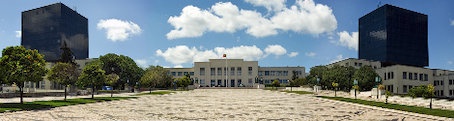
\includegraphics[width=\textwidth]{Figures/tecnico-lisboa.jpg}
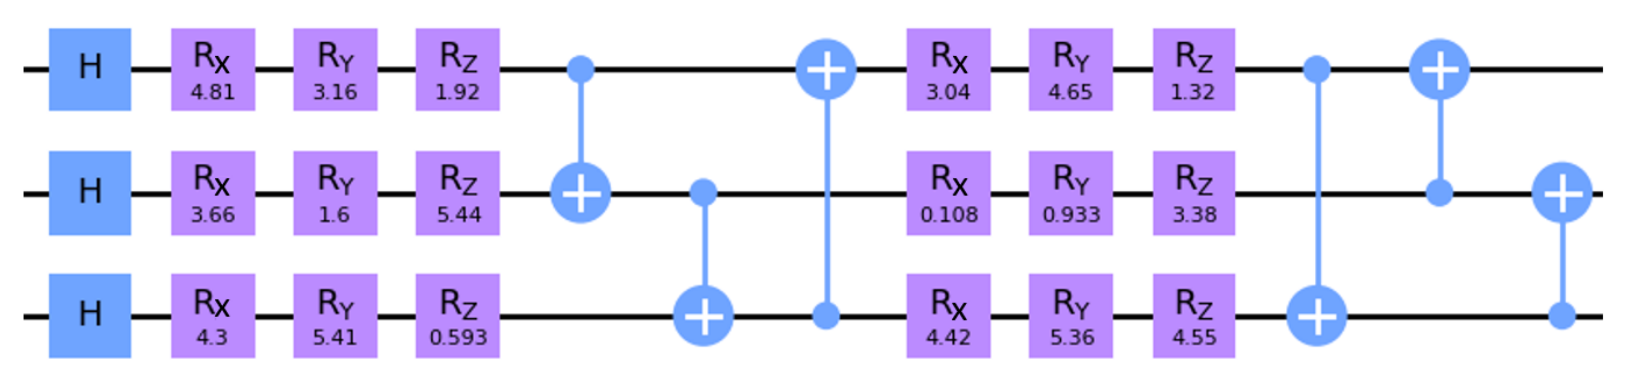
\includegraphics[width=\textwidth]{Figures/Diagrams/Strongly_Entangling_Layers.png}

% Title, author and degree
\vspace{1.0cm}
% {\FontLb Development of a new variational quantum algorithm for MaxCut: QAOA and QEMC hybrid algorithm} \\ % <<<<< EDIT TITLE. Old title.
{\FontLb iQAQE: A Framework for Variational Quantum Algorithm Development for MaxCut} \\ % <<<<< EDIT TITLE. New title.

%\vspace{0.2cm}
%{\FontMn Subtitle (optional)} \\
%\vspace{1.9cm}
\vspace{2.6cm}
{\FontMb Afonso Sequeira Azenha} \\ % <<<<< EDIT NAME
\vspace{2.0cm}
{\FontSn \coverThesis} \\
\vspace{0.3cm}
{\FontLb Engineering Physics} \\ % <<<<< EDIT COURSE
\vspace{1.0cm}
{\FontSn %
\begin{tabular}{ll}
 \coverSupervisors: & Prof. Yasser Rashid Revez Omar \\ % <<<<< EDIT NAME
                    & Prof. João Carlos Carvalho de Sá Seixas    % <<<<< EDIT NAME
\end{tabular} } \\
\vspace{1.0cm}
{\FontMb \coverExaminationCommittee} \\
\vspace{0.3cm}
{\FontSn %
\begin{tabular}{c}
\coverChairperson:     Prof. Full Name 1  \\ % <<<<< EDIT NAME
\coverSupervisor:      Prof. Full Name 2  \\ % <<<<< EDIT NAME
\coverMemberCommittee: Prof. Full Name 3     % <<<<< EDIT NAME
\end{tabular} } \\
\vspace{1.5cm}
{\FontMb June 2024} \\ % <<<<< EDIT DATE (corresponds to date of oral examination)
%
\end{center}
 % file "Thesis_FrontCover.tex"
\cleardoublepage

% ----------------------------------------------------------------------
% Dedication page (optional)
% ----------------------------------------------------------------------
%%%%%%%%%%%%%%%%%%%%%%%%%%%%%%%%%%%%%%%%%%%%%%%%%%%%%%%%%%%%%%%%%%%%%%%%
%                                                                      %
%     File: Thesis_Dedication.tex                                      %
%     Tex Master: Thesis.tex                                           %
%                                                                      %
%     Author: Andre C. Marta                                           %
%     Last modified :  2 Jul 2015                                      %
%                                                                      %
%%%%%%%%%%%%%%%%%%%%%%%%%%%%%%%%%%%%%%%%%%%%%%%%%%%%%%%%%%%%%%%%%%%%%%%%

\null\vskip5cm%
\begin{flushright}
     To Kika, my loyal companion and source of endless joy.
\end{flushright}
\vfill\newpage

 % file "Thesis_Dedication.tex"
\cleardoublepage

% ----------------------------------------------------------------------
% Declaration page (mandatory)
% ----------------------------------------------------------------------
%%%%%%%%%%%%%%%%%%%%%%%%%%%%%%%%%%%%%%%%%%%%%%%%%%%%%%%%%%%%%%%%%%%%%%%%
%                                                                      %
%     File: Thesis_Declaration.tex                                     %
%     Tex Master: Thesis.tex                                           %
%                                                                      %
%     Author: Andre C. Marta                                           %
%     Last modified :  29 Jun 2022                                     %
%                                                                      %
%%%%%%%%%%%%%%%%%%%%%%%%%%%%%%%%%%%%%%%%%%%%%%%%%%%%%%%%%%%%%%%%%%%%%%%%

\null\vskip5cm%
\begin{flushleft}
	\declarationTitle \\
	\declarationText
\end{flushleft}
\vfill\newpage

 % file "Thesis_Declaration.tex"
\cleardoublepage

% ----------------------------------------------------------------------
%  Acknowledgments (optional)
% ----------------------------------------------------------------------
%%%%%%%%%%%%%%%%%%%%%%%%%%%%%%%%%%%%%%%%%%%%%%%%%%%%%%%%%%%%%%%%%%%%%%%%
%                                                                      %
%     File: Thesis_Acknowledgments.tex                                 %
%     Tex Master: Thesis.tex                                           %
%                                                                      %
%     Author: Andre C. Marta                                           %
%     Last modified :  2 Jul 2015                                      %
%                                                                      %
%%%%%%%%%%%%%%%%%%%%%%%%%%%%%%%%%%%%%%%%%%%%%%%%%%%%%%%%%%%%%%%%%%%%%%%%

\section*{\acknowledgments}\label{sec:acknowledgments}

% Add entry in the table of contents as section
\addcontentsline{toc}{section}{\acknowledgments}

% I might want to re-read this later and make some changes (to the content, not the formatting).

First and foremost, I would like to express my deepest gratitude to my research supervisors, Prof. Yasser Omar and Prof. Zoltán Zimborás. Their invaluable guidance and support have been instrumental in shaping my research skills and scientific thinking. I am profoundly grateful for the opportunity to work with them and for the trust they have placed in me. Additionally, I am especially thankful to Prof. Yasser Omar for providing me with opportunities to broaden my horizons through international collaborations and participation in various European projects.

Equally important, if not more so, are the contributions of my colleagues Bence Bakó and Miguel Murça. Their willingness to discuss ideas and provide feedback whenever I felt lost was a tremendous support. To them, I extend my heartfelt thanks.

I would also like to extend my gratitude to my family, who have always been there for me, offering advice on both thesis-related matters and beyond.  Special thanks to my sister, Carolina, who has listened to me rant for hours on end about random quantum computing topics that she has absolutely no clue about. Although I suspect (know) that sometimes she was just pretending to listen, I appreciate the effort nonetheless.

Lastly, I would like to thank my closest friends for their unwavering support and encouragement. The small discussions with you often led to new ideas and insights, helping me view my work from different perspectives. Besides, having someone to play padel with and relax was always a welcome respite. Thank you for your companionship.

\vspace*{\fill}

This work is being developed in collaboration with Zoltán Zimborás and Bence Bako, from the Wigner Research Centre for Physics (Hungary), in the context of project: \textit{HQCC – Hybrid Quantum-Classical Computing}, supported by the EU QuantERA ERA-NET Co-fund in Quantum Technologies and by FCT -- Funda\c{c}\~{a}o para a Ci\^{e}ncia e a Tecnologia (QuantERA/004/2021).

 % file "Thesis_Acknowledgements.tex"
\cleardoublepage

% ----------------------------------------------------------------------
%  Abstract (both in English and Portuguese)
% ----------------------------------------------------------------------
%%%%%%%%%%%%%%%%%%%%%%%%%%%%%%%%%%%%%%%%%%%%%%%%%%%%%%%%%%%%%%%%%%%%%%%%
%                                                                      %
%     File: Thesis_Resumo.tex                                          %
%     Tex Master: Thesis.tex                                           %
%                                                                      %
%     Author: Andre C. Marta                                           %
%     Last modified :  4 Mar 2024                                      %
%                                                                      %
%%%%%%%%%%%%%%%%%%%%%%%%%%%%%%%%%%%%%%%%%%%%%%%%%%%%%%%%%%%%%%%%%%%%%%%%

\section*{Resumo}

% Add entry in the table of contents as section
\addcontentsline{toc}{section}{Resumo}

% Inserir o resumo em Portugu\^{e}s aqui com um máximo de 250 palavras e acompanhado de 4 a 6 palavras-chave.

Neste trabalho, apresentamos o \textit{Interpolated} \acrshort{qaoa}/\acrshort{qemc} (\acrshort{iqaqe}) \textit{Framework}, uma abordagem inovadora inspirada no \textit{Quantum Approximate Optimization Algorithm} (\acrshort{qaoa}) e no \textit{Qubit-Efficient MaxCut Heuristic Algorithm} (\acrshort{qemc}), para desenhar múltiplos Algoritmos Quânticos Variacionais (\acrshort{vqa}\textcolor{gray}{s}) distintos para resolver o problema do Corte Máximo (\acrshort{maxcut}). Este \textit{framework} baseia-se nos componentes centrais do \acrshort{qemc} enquanto integra conceitos do \acrshort{qaoa} para aproveitar os pontos fortes de ambos os algoritmos. O \textit{Framework} \acrshort{iqaqe} requer menos \textit{qubits} que o \acrshort{qaoa} e apresenta maior resiliência à incerteza estatística associada a um pequeno número de medições (\textit{shots}) em comparação com o \acrshort{qemc}.

O \textit{framework} oferece uma gama de parâmetros ajustáveis, facilitando a criação de diversos \acrshort{vqa}\textcolor{gray}{s}. Introduzimos heurísticas para a seleção desses parâmetros, como o número de \textit{qubits}, a cardinalidade das listas e os mapeamentos, e avaliamos o seu desempenho. Os nossos resultados indicam que o \acrshort{iqaqe} frequentemente apresenta um desempenho comparável ao \acrshort{qemc} e pode até superar métodos clássicos de ponta, como Goemans-Williamson, em certos cenários.

Além disso, propomos duas abordagens alternativas para resolver o problema do \acrshort{maxcut}, derivadas da nossa investigação sobre o \acrshort{iqaqe}. Embora esses métodos não se enquadrem diretamente no \textit{Framework} \acrshort{iqaqe}, oferecem \textit{insights} valiosos e potenciais caminhos para futuras pesquisas.

Também apresentamos um pequeno modelo de aprendizagem automática, projetado para determinar o mapeamento óptimo para um grafo específico com base em propriedades estatísticas dos próprios mapeamentos. Em última análise, o \textit{Framework} \acrshort{iqaqe} serve como um banco de testes versátil para o desenvolvimento de novos \acrshort{vqa}\textcolor{gray}{s}, eventualmente abrindo caminho para resultados revolucionários no futuro.

\vfill

\textbf{\Large Palavras-chave:} Computação Híbrida Quântica-Clássica (\acrshort{hqcc}), Algoritmos Quânticos Variacionais (\acrshort{vqa}\textcolor{gray}{s}), Problema do Corte Máximo (\acrshort{maxcut}), \textit{Quantum Approximate Optimization Algorithm} (\acrshort{qaoa}), \textit{Qubit-Efficient MaxCut Heuristic Algorithm} (\acrshort{qemc}).

   % file "Thesis_Resumo.tex"
\cleardoublepage

%%%%%%%%%%%%%%%%%%%%%%%%%%%%%%%%%%%%%%%%%%%%%%%%%%%%%%%%%%%%%%%%%%%%%%%%
%                                                                      %
%     File: Thesis_Abstract.tex                                        %
%     Tex Master: Thesis.tex                                           %
%                                                                      %
%     Author: Andre C. Marta                                           %
%     Last modified :  4 Mar 2024                                      %
%                                                                      %
%%%%%%%%%%%%%%%%%%%%%%%%%%%%%%%%%%%%%%%%%%%%%%%%%%%%%%%%%%%%%%%%%%%%%%%%

\section*{Abstract}

% Add entry in the table of contents as section
\addcontentsline{toc}{section}{Abstract}

% Insert your abstract here with a maximum of 250 words, followed by 4 to 6 keywords.

In this work, we introduce the Interpolated \acrshort{qaoa}/\acrshort{qemc} (\acrshort{iqaqe}) Framework, a novel approach inspired by the Quantum Approximate Optimization Algorithm (\acrshort{qaoa}) and the Qubit-Efficient MaxCut Heuristic Algorithm (\acrshort{qemc}), for designing multiple distinct Variational Quantum Algorithms (\acrshort{vqa}\textcolor{gray}{s}) to solve the Maximum Cut (\acrshort{maxcut}) problem. This framework builds on the core components of \acrshort{qemc} while integrating concepts from \acrshort{qaoa} to harness the strengths of both algorithms. The \acrshort{iqaqe} Framework requires fewer qubits than \acrshort{qaoa} and exhibits greater resilience to statistical uncertainty associated with small shot numbers compared to \acrshort{qemc}.

The framework offers a range of adjustable parameters, facilitating the creation of various \acrshort{vqa}\textcolor{gray}{s}. We introduce heuristics for selecting these parameters, such as the number of qubits, list cardinality, and mappings, and evaluate their performance. Our findings indicate that \acrshort{iqaqe} often performs on par with \acrshort{qemc} and can even surpass classical state-of-the-art algorithms like Goemans-Williamson in certain scenarios.

Additionally, we propose two alternative approaches for solving the \acrshort{maxcut} problem, derived from our investigations on \acrshort{iqaqe}. While these methods do not fall directly within the \acrshort{iqaqe} Framework, they offer valuable insights and potential avenues for future research.

We also present a small machine learning model designed to determine the optimal mapping for a specific graph based on statistical properties of the mappings themselves. Ultimately, the \acrshort{iqaqe} Framework serves as a versatile testbed for developing new \acrshort{vqa}\textcolor{gray}{s}, potentially paving the way for groundbreaking results in the future.

\vfill

\textbf{\Large Keywords:} \sloppy Hybrid Quantum-Classical Computing (\acrshort{hqcc}), Variational Quantum Algorithms (\acrshort{vqa}\textcolor{gray}{s}), Maximum Cut (\acrshort{maxcut}) Problem, Quantum Approximate Optimization Algorithm (\acrshort{qaoa}), Qubit-Efficient MaxCut Heuristic Algorithm (\acrshort{qemc}). % file "Thesis_Abstract.tex"
\cleardoublepage

% ----------------------------------------------------------------------
%  Table of contents, list of tables, list of figures and nomenclature
% ----------------------------------------------------------------------

% Table of contents
%
{ \hypersetup{hidelinks} \tableofcontents }
\cleardoublepage 

% List of tables
%
% Add entry in the table of contents as section
\phantomsection
\addcontentsline{toc}{section}{\listtablename}
% Generate list
{ \hypersetup{hidelinks} \listoftables }
\cleardoublepage 

% List of figures
%
% Add entry in the table of contents as section
\phantomsection
\addcontentsline{toc}{section}{\listfigurename}
% Generate list
{ \hypersetup{hidelinks} \listoffigures }
\cleardoublepage 

% Nomenclature
%
% Add entry in the table of contents as section
\phantomsection
\addcontentsline{toc}{section}{\nomname}
% Insert nomenclature section produced by \makenomenclature
\printnomenclature
\cleardoublepage

% Glossary
%
% Add entry in the table of contents as section
\phantomsection
\addcontentsline{toc}{section}{\acronymname}
% Insert glossary section produced by \makeglossaries
% \printnoidxglossaries[type=\acronymtype,title=\acronymname, toctitle=\acronymname]
\printnoidxglossary[type=\acronymtype,title=\acronymname, toctitle=\acronymname]
\cleardoublepage

% Set arabic numbering (1,2,...) after preface
%
\setcounter{page}{1}
\pagenumbering{arabic}

% ----------------------------------------------------------------------
%  Chapters
% ----------------------------------------------------------------------

\raggedbottom
%%%%%%%%%%%%%%%%%%%%%%%%%%%%%%%%%%%%%%%%%%%%%%%%%%%%%%%%%%%%%%%%%%%%%%%%
%                                                                      %
%     File: Thesis_Introduction.tex                                    %
%     Tex Master: Thesis.tex                                           %
%                                                                      %
%     Author: Andre C. Marta                                           %
%     Last modified :  4 Mar 2024                                      %
%                                                                      %
%%%%%%%%%%%%%%%%%%%%%%%%%%%%%%%%%%%%%%%%%%%%%%%%%%%%%%%%%%%%%%%%%%%%%%%%

\chapter{Introduction}
\label{chapter:introduction}

% Maybe, get some more references for the introduction.

% Insert your chapter material here - Talk briefly about quantum computing and its possible applications in the future. Mention quantum algorithms, hybrid quantum-classical computing, and the \acrshort{maxcut} problem.

Over the last few decades, significant progress has been achieved in the field of quantum computing. This is an entirely new computing paradigm, based on exploiting the fundamental principles of quantum mechanics to our advantage. Although the concept of a quantum computer has been around for a little over 40 years \cite{preskill2023quantum}, only rather recently, in the present century, have we successfully engineered elementary prototypes for such cutting-edge devices. Scientists and engineers worldwide are now working towards the development of practical quantum computers, which are expected to revolutionize the way we solve complex problems in various fields, such as cryptography, optimization, drug discovery, material science, machine learning, and many more.

However, with the current generation of quantum machines, so-called Noisy Intermediate Scale Quantum (\acrshort{nisq}) devices, we are still far from achieving the promised quantum advantage. This refers to the point at which a quantum computer can outperform its classical counterpart by solving specific problems considerably faster or more efficiently. It's the "holy grail" of quantum computing and what drives the research in this field forwards.

Presently, the most promising candidates for achieving meaningful quantum advantage are anchored in what has become known as "Hybrid Quantum-Classical Computing" (\acrshort{hqcc}). This approach aims to merge the strengths of both worlds: the computational power of quantum and the stability of classical computing. In this context, Variational Quantum Algorithms (\acrshort{vqa}) have been at the forefront of research, as they are particularly well-suited for near-term quantum devices, requiring fewer qubits and featuring shallower circuit depths. These algorithms are hybrid by design, using a classical optimizer to adjust the parameters of a Parameterized Quantum Circuit (\acrshort{pqc}).

Amid the many prospective applications of quantum computing, notable advances have been made in recent years in solving combinatorial optimization problems. \acrshort{vqa}\textcolor{gray}{s} like the Quantum Approximate Optimization Algorithm (\acrshort{qaoa}) \cite{farhi2014quantum} have demonstrated potential for tackling the Maximum Cut (\acrshort{maxcut}) problem, a challenging graph-based NP-hard problem in computer science. Despite its promise, however, \acrshort{qaoa} has a significant drawback: it requires a large number of qubits, exceeding the capacity of current quantum devices, when scaled to larger problem instances. This constraint has prompted the development of alternative approaches such as the Qubit-Efficient \acrshort{maxcut} Heuristic Algorithm (\acrshort{qemc}) \cite{tenecohen2023variational}, designed to address the \acrshort{maxcut} problem using fewer qubits. Meanwhile, the search for better algorithms to solve this problem continues, and the development of new hybrid quantum-classical methods is crucial to achieving quantum advantage.

%%%%%%%%%%%%%%%%%%%%%%%%%%%%%%%%%%%%%%%%%%%%%%%%%%%%%%%%%%%%%%%%%%%%%%%%
\section{Motivation}
\label{section:motivation}

% \textbf{Why do we care?}

% Relevance of the subject. - Explain why the topic is important and why it is worth studying. What would be the impact of solving the \acrshort{maxcut} problem in a more efficient manner? What are the potential applications of the results?

The search for efficient algorithms to solve combinatorial optimization problems is critical in numerous fields, such as logistics, finance, and telecommunications. The \acrshort{maxcut} problem, for example, has broad applications in areas like machine learning \cite{937505}, statistical physics \cite{Barahona_Grötschel_Jünger_Reinelt_1988}, circuit design \cite{Barahona_Grötschel_Jünger_Reinelt_1988}, and data clustering \cite{10.1007/11893318_21}. Creating more efficient algorithms to solve this problem can improve the performance of these applications, driving substantial progress in their respective fields.

Moreover, there is a strong interest from the computer science community in terms of computational complexity. The \acrshort{maxcut} problem is recognized as NP-hard, and the search for efficient algorithms to solve it may offer valuable insights into the boundaries between classical and quantum computing. It might even contribute to unraveling one of the most perplexing questions in theoretical computer science: the $P = NP$ problem. Imagining a world where the $P = NP$ conjecture is proven true, albeit improbable, is intriguing. It would mean that every problem in $NP$ could be solved in polynomial time, including \acrshort{maxcut}. This would also extend to problems like the Traveling Salesman Problem (\acrshort{tsp}) and the Knapsack Problem, among others. The implications would be profound, as this would dramatically increase our ability to solve previously difficult optimization problems, with direct applications in areas like vehicle routing, job scheduling, and broader logistics. Additionally, the impact on cryptography would be as significant – if not more so – since many cryptographic techniques rely on the complexity of $NP$ problems. For example, integer factorization is a key component of RSA (Rivest-Shamir-Adleman) encryption, a popular asymmetric encryption algorithm used extensively in public-key cryptography for secure message transmission over the internet. If $P = NP$, RSA encryption could easily be broken, leading to major security risks. Hence, the importance of studying these problems to fully understand their complexity.

The aforementioned considerations drive our efforts to develop a new algorithm for solving the \acrshort{maxcut} problem with greater efficiency and accuracy. This algorithm, the Interpolated QAOA/QEMC Hybrid Algorithm (\acrshort{iqaqe}), will be the focus of this thesis.

% Re-read this one more time, I think. I believe I end up repeating myself a bit, when I mention applications, again!

%%%%%%%%%%%%%%%%%%%%%%%%%%%%%%%%%%%%%%%%%%%%%%%%%%%%%%%%%%%%%%%%%%%%%%%%
\section{Topic Overview}
\label{section:overview}

% Briefly, dumbly, describe the topic. - Explain what variational quantum algorithms are, what QAOA and QEMC are, and what the \acrshort{maxcut} problem is. Mention the importance of hybrid quantum-classical computing and the potential of combining these two algorithms. Describe iQAQE, and how it might help in achieving the objectives.

% \textbf{What are we going to be working on?}

% Provide an overview of the topic to be studied. - Briefly describe variational quantum algorithms, QAOA and QEMC, and the \acrshort{maxcut} problem. Explain the importance of hybrid quantum-classical computing and the potential of combining these two algorithms.

In this project, we propose a new \acrshort{vqa}, the Interpolated QAOA/QEMC Hybrid Algorithm (\acrshort{iqaqe}). This algorithm combines the strengths of two existing \acrshort{vqa}\textcolor{gray}{s}, \acrshort{qaoa} and \acrshort{qemc}, for improved performance in solving the \acrshort{maxcut} problem. As previously mentioned, \acrshort{qaoa} requires a qubit for each graph vertex, making it difficult to scale. In contrast, \acrshort{qemc} uses exponentially fewer qubits by assigning one basis state to each graph node, requiring only $\log_2(n)$ qubits (for $n$ graph vertices). However, this compression leads to limitations in \acrshort{qemc}'s results. By interpolating both \acrshort{vqa}\textcolor{gray}{s}, we aim to create an algorithm that utilizes fewer qubits than \acrshort{qaoa} and performs better than \acrshort{qaoa} and \acrshort{qemc}. The new algorithm, \acrshort{iqaqe}, assigns multiple basis states to each node, unlike \acrshort{qemc}'s single basis state approach. This design tentatively allows for a more practical implementation on present-day \acrshort{nisq} devices, thanks to its reduced qubit requirements compared to \acrshort{qaoa}, fewer measurement shots than \acrshort{qemc}, and potentially greater trainability than \acrshort{qaoa}.

%%%%%%%%%%%%%%%%%%%%%%%%%%%%%%%%%%%%%%%%%%%%%%%%%%%%%%%%%%%%%%%%%%%%%%%%
\section{Objectives} % Changed from "Objectives and Deliverables" to just "Objectives" to simplify the title.
\label{section:objectives}

% Should be short. The objectives are, essentially, the same as the motivation. 'Deliverables' can either be removed, or just mention the algorithm's code (iQAQE) and the expected results.

% \textbf{What are our goals? What are we going to deliver?}

% Explicitly state the objectives set to be achieved with this thesis. - What are the main goals of the work? Mention iQAQE and how it might help in achieving the objectives.

% Also list the expected deliverables. - Results (plots, tables, etc.) and code.

The primary objective of this thesis is to develop and analyze the \acrshort{iqaqe} algorithm. The algorithm will be implemented and tested using classical simulations of quantum machines. The deliverables for this project include the \acrshort{iqaqe} algorithm's code, the results obtained from the simulations, and the analysis of these results. The expected outcomes are improvements in the performance of the \acrshort{iqaqe} algorithm compared to \acrshort{qaoa} and \acrshort{qemc}, with a focus on accuracy, efficiency, and scalability.

%%%%%%%%%%%%%%%%%%%%%%%%%%%%%%%%%%%%%%%%%%%%%%%%%%%%%%%%%%%%%%%%%%%%%%%%
\section{Thesis Outline}
\label{section:outline}

% This one is easy. Just mention the structure of the thesis.

% \textbf{What does this work's/thesis's structure look like?}

% Briefly explain the contents of each chapter.

This thesis is structured as follows: Chapter~\ref{chapter:Background} provides an overview of the background concepts related to quantum computing, variational quantum algorithms, and the \acrshort{maxcut} problem. Chapter~\ref{chapter:Base Algorithm} introduces the base hybrid quantum-classical algorithm, \acrshort{iqaqe}, explaining its design, advantages, and potential applications. Chapter~\ref{chapter:implementation} details the numerical implementation of the \acrshort{iqaqe} algorithm, including the individual algorithms \acrshort{qaoa} and \acrshort{qemc}. It also describes the benchmarking and testing methods used to evaluate the algorithm's performance. Chapter~\ref{chapter:Schemes_and_Results} presents the schemes and results obtained from the simulations, comparing \acrshort{iqaqe} with \acrshort{qaoa} and \acrshort{qemc}. It also outlines the various \acrshort{iqaqe} variations that were explored. Finally, Chapter~\ref{chapter:conclusions} concludes the thesis, summarizing the main findings and suggesting future research directions.
 % file "Thesis_Introduction.tex"
\cleardoublepage

%%%%%%%%%%%%%%%%%%%%%%%%%%%%%%%%%%%%%%%%%%%%%%%%%%%%%%%%%%%%%%%%%%%%%%%%
\raggedbottom
%                                                                      %
%     File: Thesis_Background.tex                                      %
%     Tex Master: Thesis.tex                                           %
%                                                                      %
%     Author: Andre C. Marta                                           %
%     Last modified :  4 Mar 2024                                      %
%                                                                      %
%%%%%%%%%%%%%%%%%%%%%%%%%%%%%%%%%%%%%%%%%%%%%%%%%%%%%%%%%%%%%%%%%%%%%%%%

\chapter{Theoretical background}
\label{chapter:Background}

This chapter covers the key concepts and theoretical background necessary to understand the work presented in this thesis. It begins by describing the MaxCut problem and discussing elements of computational complexity, reinforcing the rationale behind this research. The state-of-the-art algorithms for solving the MaxCut problem, both classical and quantum, are then examined. After a brief introduction to quantum computing, the chapter explores hybrid quantum-classical computing and variational quantum algorithms in greater depth. Specifically, the Quantum Approximate Optimization Algorithm (\acrshort{qaoa}) and the Qubit-Efficient MaxCut Heuristic (\acrshort{qemc}) are analyzed, as they play a pivotal role in this study.

% Include state-of-the-art somewhere?! - Maybe in the "State-of-the-Art" section. I've tried to include this in the "The Maximum Cut Problem & Computational Complexity" section.

% Insert your chapter material here.

% Some overview of the underlying theory about the topic... - Here, I should describe mathematical preliminaries, quantum computing, variational quantum algorithms, and the MaxCut problem. I should also mention the importance of hybrid quantum-classical computing and the potential of combining QAOA and QEMC. Could also make sense to mention computational complexity.

% Remember to define an acronym the first time it is used.

% The full acronym can be \acrfull{mdo}, that includes both its long definition~\acrlong{mdo} and short definition~\acrshort{mdo}.


%%%%%%%%%%%%%%%%%%%%%%%%%%%%%%%%%%%%%%%%%%%%%%%%%%%%%%%%%%%%%%%%%%%%%%%%
\section{The Maximum Cut Problem \& Computational Complexity}
\label{section:MaxCut_Comp._Complexity}

The MaxCut problem, a fundamental problem in graph theory and combinatorial optimization, involves partitioning a graph \( G = (V, E) \) into two disjoint subsets, \( S_1 \) and \( S_2 \), such that the number of edges connecting vertices from different subsets is maximized. Formally, the objective is to find a partition \( (S_1, S_2) \) that maximizes:

\begin{equation}\label{eq:Cut}
\text{Cut}(S_1, S_2) = \sum_{(u, v) \in E} \chi(u, v),
\end{equation}
where \( \chi(u, v) = 1 \) if \( u \) and \( v \) belong to different subsets, and \( \chi(u, v) = 0 \) if they belong to the same subset. This quantity is referred to as the "cut" of the partition $(S_1, S_2)$. Pictorially, this can be represented as cutting the edges of the graph (Figure \ref{fig:MaxCut}), hence the name MaxCut. What we describe here is the un-directed, un-weighted MaxCut problem. A more general formulation would involve the specific graph's adjacency matrix, $W_{ij}$.

Since the MaxCut problem is NP-hard, finding an optimal solution efficiently is a significant computational challenge, especially as the graph size grows. However, researchers have developed various approximation algorithms and heuristics to approach near-optimal solutions in a reasonable time, including both classical and quantum approaches (cf. subsections \ref{section:Classical-State-of-the-Art} and \ref{section:Hybrid-Quantum-Classical-State-of-the-Art}). These methods are designed to tackle the intrinsic complexity of the problem, providing practical solutions that have real-world applications. As mentioned earlier, the MaxCut problem finds use in a variety of fields, including machine learning \cite{937505}, statistical physics \cite{Barahona_Grötschel_Jünger_Reinelt_1988}, circuit design \cite{Barahona_Grötschel_Jünger_Reinelt_1988}, and data clustering \cite{10.1007/11893318_21}.

\begin{figure}[H]
  \centering
  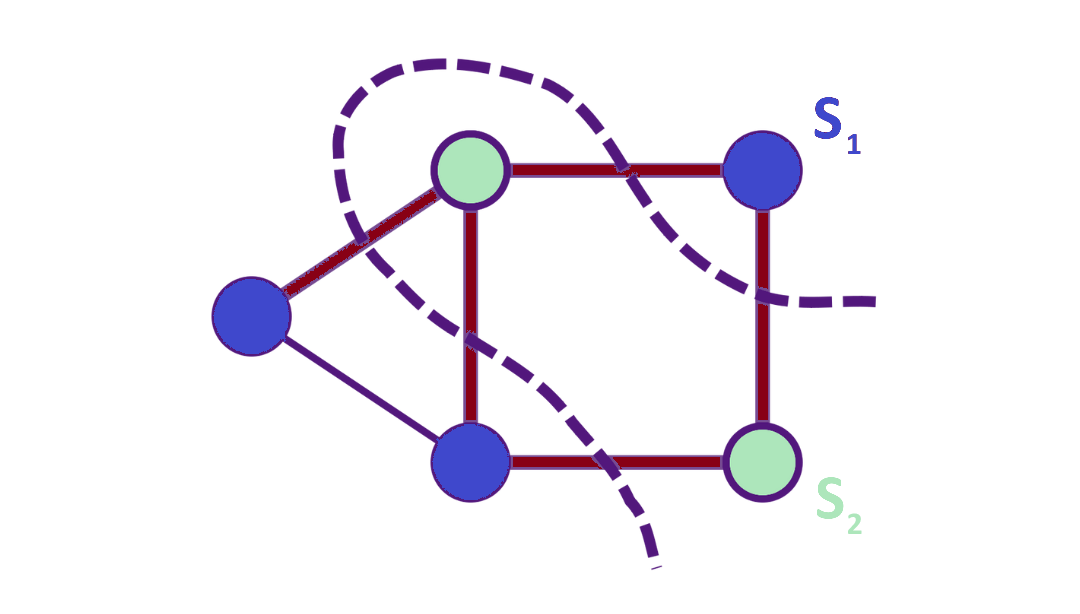
\includegraphics[width=\textwidth]{Figures/Diagrams/MaxCut.png}
  \caption{An example of a graph with a partition that maximizes the number of cut edges (red). Note that the MaxCut partition might not be unique.}
  \label{fig:MaxCut}
\end{figure}

% Discussion on Computational Complexity
We previously mentioned that the MaxCut problem is well-known to be NP-hard. (Indeed, it [decision version] even appears on Karp's original list of NP-complete problems, from 1972 \cite{Karp2010}.) Let's explore what this means in more detail. The computational complexity class of a problem is defined by the computational resources required to solve it, such as time or memory. Although there are many complexity classes (see the \href{https://complexityzoo.net/Complexity_Zoo}{Complexity Zoo}), the following four are key to our discussion:

\begin{enumerate}
  \item \textbf{P (Polynomial time)}: Problems that can be solved in polynomial time by a deterministic Turing machine, indicating they are computationally efficient.
  \item \textbf{NP (Non-deterministic Polynomial time)}: Problems that can be verified in polynomial time if given a solution, but finding the solution may not be as straightforward. Therefore, if you guess a solution, you can confirm its correctness quickly.
  \item \textbf{NP-hard (Non-deterministic Polynomial time hard)}: Problems that are at least as challenging as the most difficult problems in NP. If you could solve an NP-hard problem in polynomial time, you would be able to solve all problems in NP efficiently.
  \item \textbf{NP-complete (Non-deterministic Polynomial time complete)}: Problems that belong to NP but are also NP-hard. If you can solve one NP-complete problem efficiently, all problems in NP would become efficiently solvable.
\end{enumerate}

The MaxCut problem in its \textbf{optimization form} – "Given a graph $G$, find the maximum cut" – is NP-hard. This implies that if you could find an efficient solution to MaxCut, you could also solve all other NP problems reliably. That would include, e.g., the boolean SATisfiability problem (\acrshort{sat}), knapsack problem, decision version of the traveling salesman problem, clique problem, and more \cite{NP-problems}. This potential for broad application drives interest in developing high-performance algorithms for MaxCut. Alternatively, the MaxCut problem can be formulated as a \textbf{decision problem} – "Given a graph $G$ and an integer $k$, determine if there is a cut of size at least $k$ in $G$." This formulation is NP-complete. NP-complete status indicates that a problem is both in NP, allowing polynomial-time verification, and at least as hard as any other problem in NP, making it central to computational theory and offering crucial insights into the boundary between efficiently solvable and intractable problems. Although our focus is on the NP-hard version of the problem, it's important to understand the significance of the NP-complete formulation.

% The MaxCut problem, in particular, has a wide range of applications, such as in machine learning \cite{937505}, statistical physics \cite{Barahona_Grötschel_Jünger_Reinelt_1988}, circuit design \cite{Barahona_Grötschel_Jünger_Reinelt_1988}, and data clustering \cite{10.1007/11893318_21}.

% Describe the MaxCut problem, that we intend to solve, in an approximate manner. - Explain its importance and potential applications. Also, briefly mention computational complexity and the NP-hardness of the problem.

% MaxCut is actually NP-Hard, not NP-Complete. (Actually, depends on how you phrase it. For it to be NP-Complete, it'd have to be the decision version of the problem: "Is this the MaxCut partition?: Yes/No." I think so, but re-check this.)

% NP-Complete = NP and NP-Hard. (Instead of NP + NP-Hard.) Notation! I think I should write it like this.

%%%%%%%%%%%%%%%%%%%%%%%%%%%%%%%%%%%%%%%%%%%%%%%%%%%%%%%%%%%%%%%%%%%%%%%%
\subsection{Classical State-of-the-Art Algorithms for MaxCut}
\label{section:Classical-State-of-the-Art}

% I need to define, e.g., the concept of approximation ratio (AR). And, put it in the Glossary too!

Over the years, a variety of algorithms have been proposed to solve the MaxCut problem, ranging from exact solutions to various approximations, including heuristics and other techniques. In this work, we focus on scaling these algorithms to handle bigger graphs, which is why exact algorithms are not discussed – they quickly become impractical for large instances. Instead, our attention is on approximation algorithms, which are more suitable for larger scales\footnote{In this work, "larger/bigger graphs" will often refer to graphs with many hundreds to a few thousand nodes.}.

Approximation algorithms aim to find solutions that are close to optimal, often with a guaranteed Approximation Ratio (\acrshort{ar}). This is a measure of the performance of an approximation algorithm, representing the worst-case deviation between the algorithm's solution and the optimal solution. Formally, this can be expressed as: (For the Goemans-Williamson (\acrshort{gw}) Algorithm \cite{GW-Algorithm}, e.g.)\footnote{The actual value is $\alpha=\operatorname*{min}_{0\,\leq\,\theta\leq\pi}\,\frac{2}{\pi}\,\frac{\theta}{1\,-\,\cos\,\theta} > \,0.878$.}$$r_A^{GW} = \frac{\text{MaxCut}_{\text{GW}}}{\text{MaxCut}_{\text{Opt.}}} \approx 0.87856,$$
where $\text{MaxCut}_{\text{GW}}$ is the worst-case MaxCut value obtained by the Goemans-Williamson Algorithm, and $\text{MaxCut}_{\text{Opt.}}$ is the optimal MaxCut value. The \acrshort{ar} is a crucial metric for evaluating the quality of an approximation algorithm, providing insight into its effectiveness. The closer the \acrshort{ar} is to 1, the better the algorithm's performance. In literature, this worst-case approximation ratio might also be referred to as the \textit{performance guarantee} $\rho$, often appearing alongside designations such as $\rho$-approximation algorithms. Using this nomenclature, the Goemans-Williamson Algorithm is a $0.87856$-approximation algorithm for MaxCut (i.e., $\rho = 0.87856$).

Building on this, two commonly used \textbf{approximation algorithms} are:

\begin{itemize}
  \item \textbf{Goemans-Williamson Algorithm} \cite{GW-Algorithm}: This popular approximation algorithm achieves a performance guarantee of approximately $0.87856$, leveraging Semidefinite Programming (\acrshort{sdp}) and a randomized rounding technique. (This will be further developed below, in subsubsection \nameref{subsubsection:GW_Algorithm}.)
  \item \textbf{Spectral Methods} \cite{Spectral-MaxCut}: These techniques employ eigenvalues and eigenvectors of the adjacency matrix to identify effective cuts. While spectral methods may offer quicker computational speeds compared to other approximation strategies (e.g. \acrshort{gw}), they may not consistently provide the optimal approximation ratios. Performance-wise, the leading spectral algorithm, Trevisan's algorithm, using Soto's refined analysis \cite{Soto-MaxCut}, features a worst-case approximation ratio of $0.614$.
\end{itemize}

\textbf{Heuristic} and \textbf{metaheuristic algorithms} offer another approach, focusing on finding solutions more quickly, albeit without guaranteed approximation ratios. They are typically employed when computational efficiency is prioritized over achieving the best possible approximation ratio. These algorithms include:
\begin{itemize}
  \item \textbf{Greedy Algorithms} (Described in \cite{Spectral-MaxCut}): These build solutions incrementally, following a greedy approach. Mathematically, we start with $S_1, S_2 = \emptyset$. In each step of the algorithm, we choose a vertex $v \in V$ yet to be assigned to $S_1$ or $S_2$. Then, we add $v$ to $S_1$ or $S_2$ by choosing the larger of the two cuts $(S_1 \cup \{v\}, S_2)$ and $(S_1, S_2 \cup \{v\})$ at this step. Repeat until all vertices are assigned to a set.
  \item \textbf{Simulated Annealing} \cite{SA_MaxCut}: Employs a probabilistic optimization approach, inspired by metallurgical annealing, to iteratively explore the solution space, gradually reducing the acceptance of worse solutions ("temperature") over time to converge towards near-optimal solutions.
  \item \textbf{Genetic Algorithms} \cite{GA_MaxCut}: These algorithms, rooted in evolutionary principles, employ selection, crossover, and mutation techniques to iteratively generate solutions for the MaxCut problem, evolving from an initial population of diverse partitions towards improved solutions.
\end{itemize}

Reiterating, these approximation and heuristic methods offer scalable solutions for the MaxCut problem, making them more suitable for larger graphs where exact methods are not feasible.

Of all the mentioned approaches, we will now elaborate on the Goemans-Williamson algorithm, which currently stands as the most effective approximation method for MaxCut, boasting the best-known performance guarantee to date ($0.87856$). Its detailed explanation is particularly relevant as we plan to utilize it extensively in benchmarking our proposed algorithms later on. We opt for \acrshort{gw} over other options for one obvious reason: Our aim is to push the boundaries of MaxCut algorithms, thus it is logical to compare against the top-performing method. (We do not use any of the heuristic/metaheuristic algorithms, as they do not provide performance guarantees, and we are interested in having a benchmark to compare against.)

\subsubsection{Goemans-Williamson Algorithm}
\label{subsubsection:GW_Algorithm}

In this subsubsection, we shall present the Goemans-Williamson Algorithm in greater detail. This approximation algorithm, developed by Michel X. Goemans and David P. Williamson in 1995 \cite{GW-Algorithm}, is a cornerstone in the field of combinatorial optimization, particularly for the MaxCut problem. The algorithm leverages semidefinite programming to construct a solution that is then rounded to provide a near-optimal cut. Semidefinite programming involves optimizing a linear function of a symmetric matrix while adhering to linear equality constraints and the requirement that the matrix be positive semidefinite. This programming paradigm finds utility across diverse fields such as control theory, nonlinear programming, geometry, and combinatorial optimization, showcasing its versatility and applicability. (These applications are detailed in \cite{GW-Algorithm} and references therein.)

Formally, the Goemans-Williamson Algorithm can be described as follows. (We will use the original formulation, from \cite{GW-Algorithm}, presenting a distilled version of the most important aspects of their description.) Given a graph, with vertex set $V = \{1,..., n\}$ and non-negative weights $w_{ij} = w_{ji}$ for each pair of vertices $i$ and $j$, the weight of the maximum cut $w(S_1, S_2)$ is given by the following integer quadratic program\footnote{Note that we use the general formulation here, contemplating the possibility of weighted graphs, i.e., we do not restrict ourselves to un-weighted graphs.}:

\begin{equation}\label{eq:Graph_Cut}
  \begin{split}
  &\mathrm{Maximize}\;\;\frac{1}{2}\sum_{i<j}w_{i j}(1-y_{i}y_{j}) \\
  (Q)\qquad\qquad\qquad&\operatorname{Subject\;to:}y_{i}\in\{-1,1\}\qquad\qquad\forall i\in V.
  \end{split}
\end{equation}

\sloppy
\noindent It is clear that the sets $S_1 = \{i|y_i=1\}$ and $S_2 = \{i|y_i=-1\}$ correspond to a cut of weight $w(S_1, S_2) = \frac{1}{2}\sum_{i<j}w_{ij}\left(1-y_{i}y_{j}\right)$. This  represents the same quantity as the aforementioned $\text{Cut}(S_1, S_2) = \sum_{(u, v) \in E} \chi(u, v)$ (Eq. \ref{eq:Cut}), in the un-weighted case. Explicitly, in words, the sum in Eq. \ref{eq:Graph_Cut} is to be taken over all the graph's edges $(i, j)$, with $y_{i}$ representing node-$i$'s associated set: $y_{i}=+1$, if node-$i$ $\in S_1$, or $y_{i}=-1$, when node-$i$ $\in S_2, \forall i \in V$.

Given that solving this integer quadratic program is NP-complete \cite{GW-Algorithm}, we explore relaxations of $(Q)$. These are obtained by relaxing some of the constraints of $(Q)$, and extending the objective function to the larger space. Consequently, all solutions of $(Q)$ are feasible for the relaxation, and the optimal value of the relaxation serves as an upper bound for $(Q)$'s optimal value. We interpret $(Q)$ as constraining $y_i$ to be a $1$-dimensional unit vector. A number of possible relaxations involve allowing $y_i$ to be a multidimensional vector $v_i$ of unit Euclidean norm. As the linear space spaned by the vectors $v_i$ has dimension at most $n$ (number of graph nodes), we can assume that these vectors belong to $\mathbb{R}^{n}$. More precisely, they belong to the $n$-dimensional unit sphere, $S_n$. At this point, so as to make sure that the resulting optimization problem is, indeed, a relaxation, we must define the cost function such that it reduces to $\frac{1}{2}\sum_{i<j}w_{i j}(1-y_{i}y_{j})$ for vectors lying in a $1$-dimensional space. One way to do this is to replace $y_{i}y_{j}$ with the inner product $v_{i} \cdot v_{j}$ in the expression for $w(S_1, S_2)$. The resulting relaxation, $(P)$, reads:

\begin{equation}
  \begin{split}
  &\mathrm{Maximize}\;\;\frac{1}{2}\sum_{i<j}w_{i j}(1-v_{i} \cdot v_{j}) \\
  (P)\qquad\qquad\qquad&\operatorname{Subject\;to:}v_{i}\in S_n \qquad\qquad\forall i\in V.
  \end{split}
\end{equation}
In the context of this semidefinite programming relaxation, the \acrshort{gw} algorithm follows these steps:
\begin{enumerate}
  \item Solve $(P)$, thus obtaining an optimal set of vectors $v_{i}$;
  \item Let $r$ be a vector uniformly distributed on the unit sphere, $S_n$;
  \item Set $S_1 = \{i|v_{i} \cdot r \geq 0\}$ and $S_2 = \{i|v_{i} \cdot r < 0\}$.
\end{enumerate}
In other words, we choose a random hyperplane in $n$ dimensions, crossing through the origin, and partition the vertices according to whether the vectors $v_{i}$ lie "above" ($v_{i} \cdot r \geq 0$) or "below" ($v_{i} \cdot r < 0$) this hyperplane. Those above the hyperplane are assigned to $S_1$, and those below to $S_2$.

Furthermore, it can be shown that the \acrshort{gw} algorithm has a performance guarantee of:
\begin{equation}
  \alpha=\operatorname*{min}_{0\,\leq\,\theta\leq\pi}\,\frac{2}{\pi}\,\frac{\theta}{1\,-\,\cos\,\theta} > \,0.878.
\end{equation}
A detailed proof elucidating the appearance of this $0.878$ value is present in section $3$ of \cite{GW-Algorithm}.

Computationally, one defines the positive semidefinite matrix $X \in \mathbb{R}^{n \times n}$, with $X_{ii} = 1$ and $X_{ij} = v_{i} \cdot v_{j} = v_{i}^{T} v_j$, $\forall i, j \in V$. Then, we can solve the following semidefinite program:
\begin{equation}
  \begin{split}
  &\mathrm{Maximize}\;\;\frac{1}{2}\sum_{\text{Edges}}w_{i j}(1-X_{ij}) \\
  (N)\qquad\qquad\qquad&\operatorname{Subject\;to:}X_{ii} = 1, X \succeq 0.
  \end{split}
\end{equation}
We do possess effective tools and techniques for solving semidefinite programs, enabling the efficient determination of the optimal $X$ matrix. From there, we can extract the vectors $v_{i}$, by performing the square root operation on the matrix $X$. The resulting matrix's columns, or lines – $X$ is symmetric – will correspond to the desired vectors $v_{i}$. This outlines the process for solving $(P)$ as listed earlier.

% Re-read all of this and potentially re-write some things. I'm also not sure if I should just cite the GW paper, for defining semidefinite programming.

% Describe the state-of-the-art algorithms for the MaxCut problem. - Mention classical algorithms, such as the Goemans-Williamson algorithm, and quantum algorithms, such as the Quantum Approximate Optimization Algorithm (QAOA) and the Qubit-Efficient MaxCut Heuristic (QEMC) algorithm.

%%%%%%%%%%%%%%%%%%%%%%%%%%%%%%%%%%%%%%%%%%%%%%%%%%%%%%%%%%%%%%%%%%%%%%%%

\subsection{Hybrid Quantum-Classical State-of-the-Art Algorithms for MaxCut}
\label{section:Hybrid-Quantum-Classical-State-of-the-Art}

A number of different hybrid quantum-classical algorithms have been proposed to solve the MaxCut problem, leveraging the unique properties of quantum computing to potentially outperform purely classical algorithms. They are designed to exploit quantum superposition and entanglement to explore the solution space more efficiently. In this section, we will briefly mention the state-of-the-art hybrid quantum-classical algorithms for MaxCut, focusing on the Quantum Approximate Optimization Algorithm (\acrshort{qaoa}) and the Qubit-Efficient MaxCut Heuristic Algorithm (\acrshort{qemc}). Due to their variational nature, these algorithms do not have a theoretical performance guarantee, but they have shown promising results in practice.

Presently, the Quantum Approximate Optimization Algorithm (\acrshort{qaoa}), initially introduced in \cite{farhi2014quantum}, is one of the top candidates for achieving meaningful quantum advantage with near-term quantum devices. Although, MaxCut-wise, it has a substantial limitation: it requires a number of qubits equal to the number of graph nodes. This is a significant drawback, as it severely limits the algorithm's scalability to bigger graphs. Hence, why it is believed that "QAOA for Max-Cut requires hundreds of qubits for quantum speed-up" \cite{Guerreschi2019}. After all, our classical algorithms work just fine for small graphs, which is why we do not present performance metrics for basic \acrshort{qaoa}. Alternatively, different \acrshort{qaoa} variations have been proposed to address the issue of high qubit requirements, such as QAOA-in-QAOA \cite{zhou2022qaoainqaoa}, which partitions a large graph into many smaller subgraphs, each of which is easily solved using a separate \acrshort{qaoa} instance. Afterwards, these results are joined together by working through another, this time \textbf{weighted}, MaxCut problem. This approach in particular has proven to yield competitive or even better performance over the best known classical algorithms, i.e. \acrshort{gw}, for graphs up to $2000$ nodes.

A separate problem one might face when implementing \acrshort{qaoa}, that also hinders its application to larger graphs, has to do with qubit connectivity\footnote{Qubit connectivity refers to the pattern or arrangement of connections between qubits in a quantum computing system, determining which qubits can interact directly with each other.}, as \acrshort{qaoa} might require specific connectivity patterns that are not natively available in present-day \acrshort{nisq} devices. To implement these, we are often required to utilize a number of $2$-qubit SWAP gates, which degrade the algorithm's performance by introducing extra noise in the system, and hence errors in our results. Therefore, a parallel line of work has been to develop \acrshort{qaoa} variations that have lesser connectivity requirements, in the sense that they do not depend on arbitrary qubit connectivity. For example, Parity-QAOA \cite{ender2022modular,Ender2023parityquantum} was designed for quantum chips with planar lattice geometry (Figure \ref{fig:Planar_lattice_geometry}), requiring only nearest-neighbour connectivity. Although it necessitates more qubits, it entirely solves this problem.

\begin{figure}[H]
  \centering
  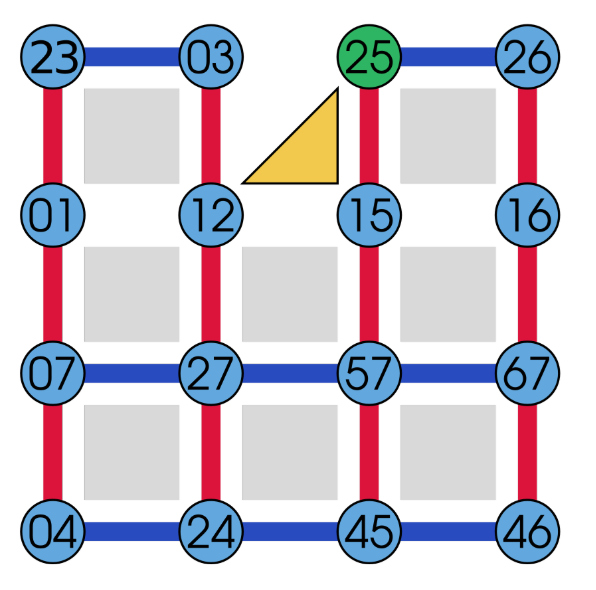
\includegraphics[width=0.5\textwidth]{Figures/Diagrams/Planar_lattice_geometry.png}
  \caption{Planar lattice geometry illustration: the circular nodes represent the physical qubits, each of which can interact directly with its nearest neighbours. The lines represent terms of the driver Hamiltonian, from Parity-QAOA \cite{ender2022modular}. The numbers refer to edges in the original graph. Image reproduced from \cite{ender2022modular}.}
  \label{fig:Planar_lattice_geometry}
\end{figure}

Furthermore, the Qubit-Efficient MaxCut Heuristic Algorithm (\acrshort{qemc}), introduced in \cite{tenecohen2023variational}, is a quantum-classical hybrid algorithm that aims to solve the MaxCut problem using fewer qubits than \acrshort{qaoa}, therefore extending its applicability to larger graphs. It has shown cutting-edge performance in practice, surpassing the classical state-of-the-art, i.e. \acrshort{gw}, for graphs up to $2048$ nodes. The novelty of this algorithm is that it opens up the door for quantum devices to be used for large MaxCut instances, previously unfeaseble due to qubit number limitations, which rendered \acrshort{qaoa} computations for such large graphs impossible. As was already mentioned, \acrshort{qemc} allows for an exponential compression in the number of needed qubits, enabling its utilization on today's quantum hardware for considerably larger graphs than what would be possible with traditional \acrshort{qaoa}. However, this exponential compression also makes it efficiently simulable classically, which effectively defeats its purpose as a quantum algorithm. For this reason, \acrshort{qemc} is termed a quantum-inspired classical algorithm and, by definition, will not produce any quantum advantage. Either way, we include it in this subsection, since it can always be implemented as a \acrshort{vqa} on current-day \acrshort{nisq} devices.

More recently, different algorithms have been proposed in an attempt to reduce the number of qubits required for larger graphs, without falling into the trap of efficient classical simulability. (After all, we are looking for quantum advantage.) Polynomial compression-based algorithms, such as that proposed in \cite{sciorilli2024largescale}, have too shown promising results. This one in specific \cite{sciorilli2024largescale} is, to the best of our knowledge, boasting the highest quality attained experimentally on sizes up to $7000$ graph nodes, competitive with state-of-the-art classical solvers. Not only that, but their specific qubit-efficient encoding brings in a super-polynomial mitigation of barren plateaus\footnote{In \acrshort{vqa} analysis, barren plateaus are characterized by a vanishing expectation value of $\nabla{\mathcal{L}}$ over random parameter initializations and an exponential decay (in $n$) of its variance. Note that $\mathcal{L}$ refers to the loss function. These are, thus, flat regions of the parameter space, impeding optimization.} as a built-in feature, which constitutes a significant advantage over other \acrshort{vqa}\textcolor{gray}{s}. Curiously enough, our initial idea for the \acrshort{iqaqe} algorithm is quite similar to what is explored in \cite{sciorilli2024largescale}. However, we believe our algorithm to be somewhat more general, by not assuming \textit{a priori} a polynomial compression in the number of qubits.

% I believe this part is okay, now. Maybe re-read it one more time, and ask Carolina to do the same. Add the Parity-QAOA figure, illustrating planar lattice geometry?

% Find papers showing that QAOA has been used/employed for solving MaxCut in x graphs.

% Describe, albeit briefly, the state-of-the-art quantum algorithms for the MaxCut problem. - Mention the Quantum Approximate Optimization Algorithm (QAOA) and the Qubit-Efficient MaxCut Heuristic (QEMC) algorithm. No need to explain them, as they will be further developed in the next sections.

%%%%%%%%%%%%%%%%%%%%%%%%%%%%%%%%%%%%%%%%%%%%%%%%%%%%%%%%%%%%%%%%%%%%%%%%
\section{Quantum Computing Primer}
\label{section:QC_Primer}

In this section, we present a brief introduction to quantum computing, focusing on its fundamental ideas and principles. We begin with an overview of the general concepts, followed by a discussion of quantum gates and circuits, crucial for understanding quantum algorithms. This groundwork will prepare us to delve into the specifics of variational quantum algorithms and their application to the MaxCut problem.

% I feel like I should add some more mathematics to this. Refer to Bence's master thesis as a reference, e.g. Done!

% Remember to go over the papers in the 'papers' folder! Add those that aren't there yet! Maybe re-check whether to include some of the 'misc' references (IonQ/Google qubit-types, e.g. Isn't there a paper where this is refered?) I should try to replace these with actual papers. The Pennylane tutorials are fine though, I think. They even provide their references, which can be cross-checked any time. For the Google, i.e., can utilize the Sycamore paper, for quantum advantage. There's probably something similar for IonQ, and others (maybe not quantum advantage, but still). Update: this is done!

% Change all the important people's names to italics? I've removed italics from everyone's names now. Done!

% Remember that we have an 80 page maximum limit! This can be extended to 100 in appendices, and the like.

\subsection*{General concepts and mathematical formalism}
\vspace*{-5mm}{\scriptsize \noindent (This description is inspired by \cite{nielsen2010quantum}.)}

Quantum computing makes use of the foundational principles of quantum mechanics in an attempt to extract some sort of quantum advantage from them. Instead of using classical binary digits, quantum computers use their quantum analog, qubits. In practice, qubits can be any two-state quantum system. Said states are, unequivocally, associated with the states $\ket{0}$ and $\ket{1}$, conventionally, very much like in classical computing when one uses bits. The primary distinction lies in the fact that a qubit, being a quantum system, can exist in a superposition of both states generally denoted as:
\begin{equation}
  \mathcal{H}^2 \ni \ket{\psi} = \alpha \ket{0} + \beta \ket{1},
\end{equation}
where $\alpha, \beta \in \mathbb{C}$, with $\abs{\alpha}^2 + \abs{\beta}^2 = 1$. This ensures probability normalization to $1$, as, according to the famous Born rule, the probability of measuring the qubit in state $\ket{0}$ is $\abs{\bra{0}\ket{\psi}}^2 = \abs{\alpha}^2$, and in state $\ket{1}$ is $\abs{\bra{1}\ket{\psi}}^2 = \abs{\beta}^2$.

In the same vein, one can compose (represented by the tensor product) $n$ qubits to obtain an $n$-qubit state:
\begin{equation}\label{eq:n_qubit_state}
  \ket{\psi}=\bigotimes_{i=0}^{n-1}(\alpha_{i}\ket{0}\ +\beta_{i}\ket{1}).
\end{equation}
More generally, we can express an arbitrary pure state of $n$ qubits, $\ket{\psi}$, by a normalized linear combination of the computational basis states $\ket{b_0 b_1 ... b_{n-1} b_n} \coloneq \ket{b_0} \otimes \ket{b_1} \otimes ... \otimes \ket{b_{n-1}} \otimes \ket{b_n}$:
\begin{equation}\label{eq:general_n_qubit_state}
  \ket{\psi} = \sum_{\boldsymbol{b} \in \{0, 1\}^{\otimes n}} \alpha_{\boldsymbol{b}} \ket{b_0 b_1 ... b_{n-1} b_n},
\end{equation}
where $\sum_{\boldsymbol{b} \in \{0, 1\}^{\otimes n}} \abs{\alpha_{\boldsymbol{b}}}^2 = 1$. This superposition phenomenon (mathematically characterized by the linear combination of basis states), utterly impossible in classical physics, brings unprecedented computational power under certain scenarios, as it introduces a kind of built-in parallelism in quantum computing, a highly desirable feature for any computational scheme.

In addition to this, quantum computing also exploits entanglement as a resource. Entanglement allows for intricate correlations between qubits, which have no classical counterpart and are believed to offer computational speed-ups, although it is yet unclear exactly how. An entangled state, by definition, is one that cannot be expressed as the tensor product of individual qubit states, i.e., it cannot be represented in the form of Eq. \ref{eq:n_qubit_state}. The most famous example of entangled states are the Bell states, representing what are known as two-qubit (or bipartite) maximally entangled states. Such Bell states are reproduced below:
\begin{equation} % Check if these are correct!
  \begin{aligned}
  \ket{\Phi^+} &= \frac{1}{\sqrt{2}}(\ket{00} + \ket{11}), \quad
  \ket{\Phi^-} = \frac{1}{\sqrt{2}}(\ket{00} - \ket{11}), \\
  \ket{\Psi^+} &= \frac{1}{\sqrt{2}}(\ket{01} + \ket{10}), \quad
  \ket{\Psi^-} = \frac{1}{\sqrt{2}}(\ket{01} - \ket{10}).
  \end{aligned}
\end{equation}
Clearly, these states cannot be expressed as a tensor product of two individual qubit states. From a practical standpoint, Bell states frequently serve as foundational elements in advanced techniques like quantum teleportation and quantum cryptography. Quantum Key Distribution (\acrshort{qkd}) protocols, for example, frequently rely on entangled Bell pairs to distribute secure keys for encrypting and decrypting messages.

Another key topic in quantum information theory is the distinction between pure and mixed states. So far, we have only been treating pure states, which are represented by a single ket vector in some Hilbert space. Mixed states, on the other hand, are represented by density matrices, which are positive semidefinite matrices with unit trace. These matrices are used to describe a statistical ensemble of quantum states. The density matrix $\rho$ of a quantum state $\ket{\psi}$ is defined as:
\begin{equation}
  \rho = \dyad{\psi}{\psi}.
\end{equation}
In the more general case of a statistical ensemble of states $\ket{\psi_i}$, each with probability $p_i$, the density matrix $\rho$ is given by:
\begin{equation}
  \rho = \sum_i p_i \dyad{\psi_i}{\psi_i}.
\end{equation}
It's crucial to avoid confusing this with superposition, as a mixed state comprises a statistical ensemble of pure states, while superposition pertains to a single state that is a linear combination of other states. For instance, the state $\ket{\psi_S} = \frac{1}{\sqrt{2}}\left(\ket{0} + \ket{1}\right)$ represents a superposition of $\ket{0}$ and $\ket{1}$, whereas the state $\rho_M = \frac{1}{2}\left(\dyad{0}{0} + \dyad{1}{1}\right)$ denotes a mixed state, signifying that half the states in the ensemble are in state $\ket{0}$ and the other half in state $\ket{1}$. Unlike the probabilistic mixture ($\rho_M$), the superposition ($\psi_S$) can exhibit quantum interference, hence why it is important to distinguish between the two. If desired, this distinction can also be observed in the off-diagonal terms of the density matrix, referred to as coherences, which are responsible for quantum interference effects: the off-diagonal terms of $\rho_{M}$ are zero, whereas those of $\rho_{S} = \ket{\psi_S}\bra{\psi_S} = \frac{1}{4}\left(\dyad{0}{0} + \dyad{0}{1} + \dyad{1}{0} + \dyad{1}{1}\right)$ are not.

Currently, numerous quantum computing architectures are in competition and the ultimate victor remains uncertain. Nevertheless, the most prominent architectures have qubits composed of either photons \cite{slussarenko2019photonic, Xanadu_Photonics}, neutral atoms (using Rydberg states) \cite{Henriet2020quantumcomputing, Wu_2021}, trapped ions \cite{bruzewicz2019trapped}, semiconductors (still in their infancy), or, most notably, superconducting circuits \cite{Huang_2020, SC_Qubits} – employed by giants like IBM and Google in their quantum processors. Looping back to the definition of a qubit, considering a photonic quantum computer, it becomes rather straightforward and natural to map the photons' vertical and horizontal polarizations to the $\ket{0}$ and $\ket{1}$ states, respectively. Once again, this mapping is analogous to how classical computing maps the current/no current states to 1 and 0.

The next step is to understand how these so-called quantum circuits act on our qubits, and how they can be used to perform quantum computations. This is where quantum gates come into play.

% Things that are yet to be done in regards to this section:
% Mention the Hadamard gate somewhere! It's a fundamental gate in quantum computing. Done!

% Present proof? Using only R_x and R_z, I know this is possible. Done!

% Wikipedia link? Find something else, maybe? Probably. Done!

\subsection*{Quantum gates and circuits}
Presently, quantum computers are being designed predominantly with a circuit-based architecture. These circuits serve as the quantum equivalent of classical logic circuits, however, instead of the typical AND, OR, and NOT gates, quantum circuits feature quantum gates. These gates apply specific transformations to qubits, based on their definitions, taking an initial state $\ket{\psi}$ to an output state $\ket{\phi} = U\ket{\psi}$, for some gate $U$, \textbf{designed to be unitary}, i.e., $U^{\dagger}U = UU^{\dagger} = I$, where $I$ is the identity matrix. Unitary transformations preserve the normalization of quantum states and the inner product between states, which are essential properties in quantum mechanics. Additionally, they ensure that quantum operations are reversible, meaning that information is not lost during computation. This [unitary gates] can also be seen as a natural consequence of the Schrödinger equation, governing the time evolution of quantum systems, requiring said evolution to be described by a unitary operator.

The most frequently used quantum gates consist of rotations around each of the three Cartesian axes, represented as complex exponentials of the Pauli $x$, $y$ and $z$ matrices ($\sigma_x$, $\sigma_y$ and $\sigma_z$). The Pauli matrices are defined as: (Note the alternative notation, $\boldsymbol{X}$, $\boldsymbol{Y}$ and $\boldsymbol{Z}$, for the sake of clarity.)
\begin{equation}
  \boldsymbol{X} \coloneq \sigma_x =
  \begin{pmatrix}
    0 & 1 \\
    1 & 0
  \end{pmatrix},
  \quad
  \boldsymbol{Y} \coloneq \sigma_y =
  \begin{pmatrix}
    0 & -i \\
    i & 0
  \end{pmatrix},
  \quad
  \boldsymbol{Z} \coloneq \sigma_z =
  \begin{pmatrix}
    1 & 0 \\
    0 & -1
  \end{pmatrix}.
\end{equation}
Furthermore, when we mention rotations, these are to be seen in the Bloch sphere, which is a geometrical representation of the pure state space of a two-level quantum system, an illustration of which can be seen in Figure \ref{fig:Bloch_sphere}.

\begin{figure}[H]
    \centering
    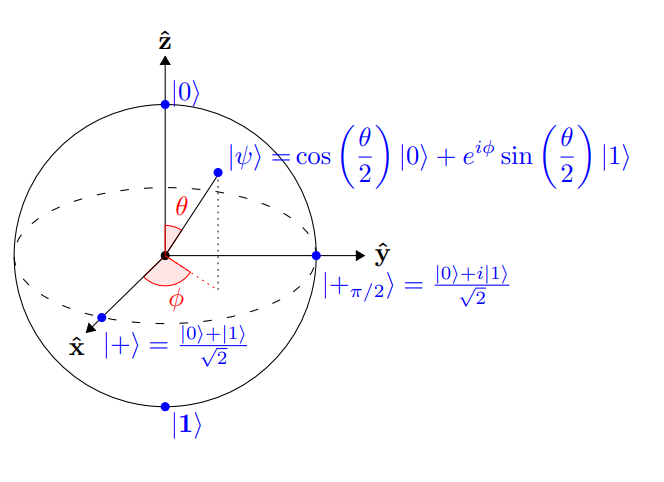
\includegraphics[width=0.75\textwidth]{Figures/Diagrams/Bloch_sphere.png}
    \caption{Bloch sphere representation. The sphere's north  and south poles correspond to states $\ket{0}$ and $\ket{1}$, respectively. Reproduced from \cite{Bloch_Sphere_Ref}.}
    \label{fig:Bloch_sphere}
\end{figure}
\noindent The aforementioned rotation gates can be written as: $R_x(\theta) = e^{-i\theta\sigma_x/2}$, $R_y(\theta) = e^{-i\theta\sigma_y/2}$, and $R_z(\theta) = e^{-i\theta\sigma_z/2}$. In matrix form, this reads:
\begin{equation}
  \resizebox{0.90\hsize}{!}
  {$
  % X rotation matrix
  R_x(\theta) =
  \begin{pmatrix}
    \cos\left(\frac{\theta}{2}\right) & -i\sin\left(\frac{\theta}{2}\right) \\
    -i\sin\left(\frac{\theta}{2}\right) & \cos\left(\frac{\theta}{2}\right)
  \end{pmatrix},
  \quad
  % Y rotation matrix
  R_y(\theta) =
  \begin{pmatrix}
    \cos\left(\frac{\theta}{2}\right) & -\sin\left(\frac{\theta}{2}\right) \\
    \sin\left(\frac{\theta}{2}\right) & \cos\left(\frac{\theta}{2}\right)
  \end{pmatrix},
  \quad
  % Z rotation matrix
  R_z(\theta) =
  \begin{pmatrix}
    e^{-i\frac{\theta}{2}} & 0 \\
    0 & e^{i\frac{\theta}{2}}
  \end{pmatrix},
  $}
\end{equation}
These will frequently appear in quantum circuits, as they are the most basic quantum gates, in the sense that all other single-qubit gates can be re-constructed from them. I.e., for any unitary single-qubit gate $U$, one can always find a decomposition $U=e^{i\phi}R_{Z}(\gamma)R_{X}(\beta)R_{Z}(\alpha)$ (proven in \cite{Barenco_1995}).
% Present proof? Using only R_x and R_z, I know this is possible. I should present a reference for this, though. Done!

For illustrative purposes, to elucidate how single-qubit gates act on qubits, it is quite simple to verify that the $\sigma_x$ matrix (alternative symbol, $\boldsymbol{X}$) behaves exactly like a NOT gate. This correspondence is established through a $180^{\circ}$ rotation around the $x-$axis. Mathematically,
% X|0> = |1> 
\begin{equation}
\boldsymbol{X} = 
\begin{pmatrix}
0 & 1 \\
1 & 0
\end{pmatrix},
\end{equation}
such that:
\begin{equation}
\boldsymbol{X}\ket{0}
=
\begin{pmatrix}
0 & 1 \\
1 & 0
\end{pmatrix}
\begin{pmatrix}
1 \\
0
\end{pmatrix}
=
\begin{pmatrix}
0 \\
1
\end{pmatrix}
=
\ket{1}.
\end{equation}
Another essential gate found in most quantum algorithms is the Hadamard gate. It can be represented as the following linear combination of $\boldsymbol{X}$ and $\boldsymbol{Z}$ matrices: $H = \frac{1}{\sqrt{2}}\left(\boldsymbol{X} + \boldsymbol{Z}\right)$, and is particularly useful for creating superpositions, as it maps the state $\ket{0}$ to $\frac{1}{\sqrt{2}}(\ket{0} + \ket{1}) \coloneq \ket{+}$, and $\ket{1}$ to $\frac{1}{\sqrt{2}}(\ket{0} - \ket{1}) \coloneq \ket{-}$.
% Re-read this bit on the Hadamard gate.

In addition to these simple one-qubit quantum gates, there are also gates designed for multiple qubits. For instance, consider the controlled-NOT gate (CNOT), which does exactly what its name suggests: if the control qubit is in state $\ket{1}$, it applies NOT to the test qubit, whereas if it is in state $\ket{0}$ instead, nothing happens. The CNOT gate is also quite prevalent in quantum circuits, playing a vital role in creating entanglement between qubits, which is a crucial resource in quantum computing. The circuit representation and equivalent matrix form of the CNOT gate are presented below, in Figure \ref{fig:CNOT}.

\begin{figure}[htbp]
  \centering
  \begin{subfigure}[t]{0.45\textwidth}
      \centering
      
\includegraphics[width=.75\textwidth]{Figures/Diagrams/CNOT_Gate.png}
      \caption{CNOT gate – Circuit representation. The black circle identifies the control qubit. The other qubit is the test qubit.}
      \label{fig:CNOT_Gate}
  \end{subfigure}
  \hfill
  \begin{subfigure}[t]{0.45\textwidth}
      \centering
      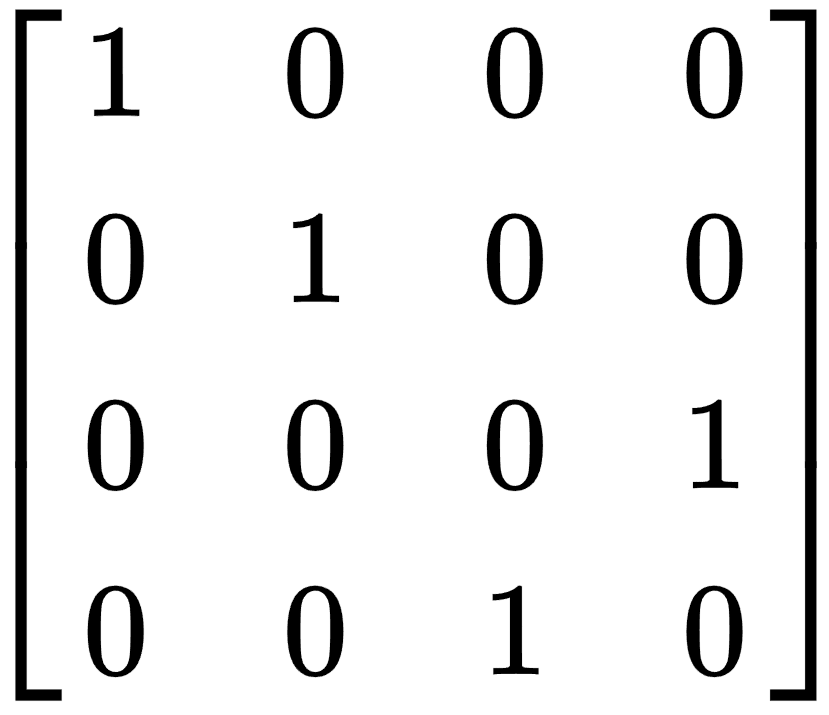
\includegraphics[width=.50\textwidth]{Figures/Diagrams/CNOT_Matrix.png}
      \caption{CNOT gate – Equivalent matrix form.}
      \label{fig:CNOT_Matrix}
  \end{subfigure}
  \caption{Two-qubit gate example – The controlled-NOT gate.}
  \label{fig:CNOT}
\end{figure}

More generally, within a quantum circuit, an intricate network of interconnected qubits and gates collaborates to execute a specific algorithm. For example, the circuit depicted in Figure \ref{fig:QCircuit}, below, is designed for the implementation of the renowned Grover's search algorithm \cite{Grover}.

% Taken from Wikipedia. Should, then, include everything in my references!
\begin{figure}[H]
    \centering
    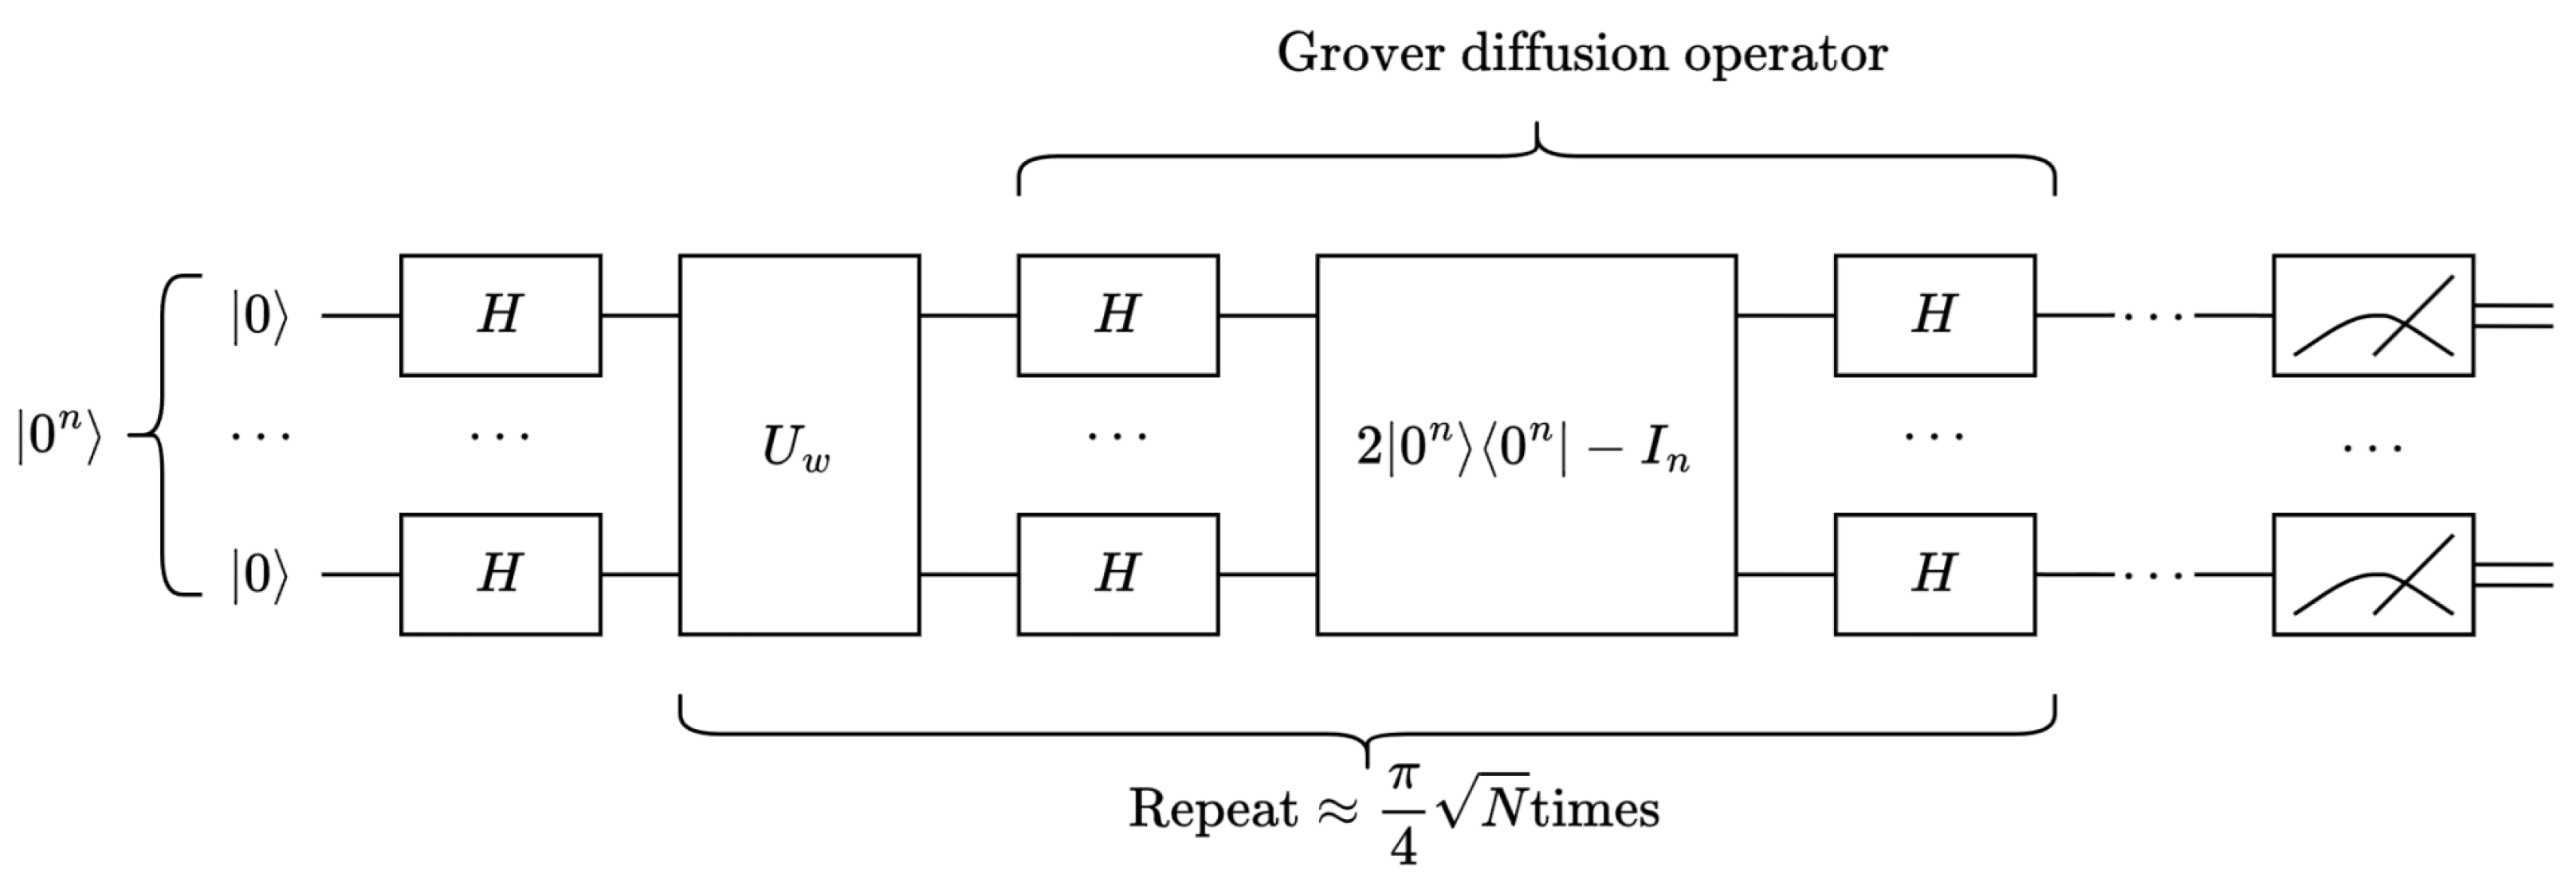
\includegraphics[width=\textwidth]{Figures/Diagrams/Grover_Circuit.png}
    \caption{Quantum circuit utilized in the famous Grover's search algorithm \cite{Grover}. Integraly reproduced from \cite{e26030216}.}
    \label{fig:QCircuit}
\end{figure}
This is a purely quantum algorithm, different from what we intend to explore in this work. Nevertheless, it serves as a good example of how quantum circuits can be used to implement complex quantum algorithms.

An additional point of interest is the potential for classical simulation of quantum circuits. Quantum gates, being akin to mathematical operators, can always be expressed in matrix form. Consequently, analyzing the impact of a series of quantum gates, i.e., a quantum circuit, on a specific quantum state is achievable by sequentially applying the relevant operators, as they appear in the circuit. At the end of this process, we arrive at a quantum state typically distinct from the initial state. This entire simulation can be executed classically. However, its scalability is severely limited, as the number of states, constituting our computational basis, representable with $n$ qubits grows exponentially, at a rate of $2^n$. As one might anticipate, this very quickly becomes unmanageable. Eventually, either memory constraints impede the storage of such extensive states, or the computations slow down to a point where the endeavor loses practicality. Effectively, simulating quantum computers becomes challenging beyond a few dozen qubits. Some tabletop calculations suggest that simulating $28$ qubits would necessitate approximately $13$ GB of memory, reaching the theoretical maximum capacity of a modern standard $16$ GB personal computer. It's important to note that for each additional qubit, memory requirements double. For instance, simulating $50$ qubits would demand about $54$ Petabytes of memory, and for $51$ qubits, approximately $108$ PB, and so forth. These estimations are based on the assumption that a complex number is stored as two Python floats, each requiring $24$ bytes of memory, thus a complex amplitude requires $48$ bytes of memory to be stored. Then, one such amplitude is required for each of the $2^{n}$ basis states, for $n$ qubits.

% This could be "Quantum Computing".

% The research should be supported with a comprehensive list of references.
% These should appear whenever necessary, in the limit, from the first to the last chapter.

% Regarding the exponential scaling: maybe it'd be interesting to provide some numbers. In other words, try to find the "greatest" number of qubits one can classically simulate, at the moment, and connect this to a number of bytes (memory-wise): Some Exabytes?

% I feel like if I am going to be including some text from my PIC2 report, I should further explain some of these things better.

% A reference can be cited in any of the following ways:
% %
% \begin{itemize}
%   \item Citation mode \#1 - \quad \cite{Marta:AeroBest2021}
%   \item Citation mode \#2 - \quad \citet{Marta:AeroBest2021}
%   \item Citation mode \#3 - \quad \citep{Marta:AeroBest2021}
%   \item Citation mode \#4 - \quad \citet*{Marta:AeroBest2021}
%   \item Citation mode \#5 - \quad \citep*{Marta:AeroBest2021}
%   \item Citation mode \#6 - \quad \citealt{Marta:AeroBest2021}
%   \item Citation mode \#7 - \quad \citealp{Marta:AeroBest2021}
%   \item Citation mode \#8 - \quad \citeauthor{Marta:AeroBest2021}
%   \item Citation mode \#9 - \quad \citeyear{Marta:AeroBest2021}
%   \item Citation mode \#10 - \quad \citeyearpar{Marta:AeroBest2021}
% \end{itemize}

% The references may include books~\cite{Marta:AeroBest2021}, articles in journals~\cite{Morgado:2022:SAMO}, part of a collection of books~\cite{jameson:adjointns}, articles in conferences~\cite{Alves:ICUAS:2022}, master theses~\cite{Pacheco:MSc} and PhD theses~\cite{Rodrigues:PhD}.

% Several citations can be made simultaneously as \cite{Campos:2021:QJMAM,Alexandre:2020:PLOS}.

% This is often the default bibliography style adopted (numbers following the citation order), according to the options:

% {\tt \textbackslash usepackage\{natbib\}} in file {\tt Thesis\_Preamble.tex},\\
% {\tt \textbackslash bibliographystyle\{abbrvnat\}} in file {\tt Thesis.tex}.\\

% Notice however that this style can be changed from numerical citation order to authors' last name with the options:

% {\tt \textbackslash usepackage[numbers]\{natbib\}} in file {\tt Thesis\_Preamble.tex},\\
% {\tt \textbackslash bibliographystyle\{abbrvunsrtnat\}} in file {\tt Thesis.tex}. \\

% Multiple citations are compressed when using the {\tt sort\&compress} option when loading the {\tt natbib} package as {\tt \textbackslash usepackage[numbers,sort\&compress]\{natbib\}} in file {\tt Thesis\_Preamble.tex}, resulting in citations like \cite{Pacheco:2024:JAUTO,Portugal:2024:MODELLING,Matos:2022:AEROSPACE,Rodrigues:2020:SAMO,Rodrigues:2019:RENE,Campos:2018:JSV,Rodrigues:2018:CAF,Campos:2015:GAFD,Marta:2014:JPP,Rodrigues:2014:SMO,Campos:2014:IJMS,Marta:2013:AIAAJ,Marta:2013:CAF,Marta:2010:CAF,Marta:2007:IJCFD}.


%%%%%%%%%%%%%%%%%%%%%%%%%%%%%%%%%%%%%%%%%%%%%%%%%%%%%%%%%%%%%%%%%%%%%%%%
\section{Hybrid Quantum-Classical Computing}
\label{section:HQCC}

% Other models. - Variational quantum algorithms, Parameterized quantum circuits, etc.

Hybrid quantum-classical computing refers to a computational approach that combines elements of both classical and quantum computing paradigms to leverage the strengths of each. In this model, classical processors and quantum processors work in tandem to solve complex problems more efficiently than either could achieve alone. This collaborative strategy aims to harness quantum computing's unique capabilities while mitigating the challenges and limitations associated with quantum systems, such as error correction and decoherence. As of today, the synergy between classical and quantum elements holds promise for addressing complex real-world problems in areas like optimization, machine learning, and cryptography (cf. Figure \ref{fig:VQAs_Applications}).

\subsection{Variational Quantum Algorithms}
\label{subsection:VQA}

% I've only just copied things from my PIC2 report. I still need to re-read everything and add more information, if I so deem important. Even this copy-paste'ing isn't done yet. Put this in a private GitHub repo., I think. [Good, for security reasons, in case somethings happens, I have a backup.] Done!

% In describing Ansätze, I should mention that, in general, it is always better to use problem-inspired Ansätze. If they're well designed/implemented, they should always yield better results. Also, when presenting examples of Ansätze, I can show some images of those. Done!

% I should fact check some of what I say in the PIC2 report regarding problem-agnostic and -inspired Ansätze. I feel like I might have said something wrong there. [About parameter number and depth, mostly, and, thus trainability.]

The hallmark of \acrshort{hqcc} is what are called variational quantum algorithms (\acrshort{vqa}\textcolor{gray}{s}), which correspond to hybrid quantum-classical algorithms, typically realized through a parameterized quantum circuit (\acrshort{pqc}). Additionally, as part of their implementation, the parameters are subjected to training in order to achieve the desired outcomes, by minimizing the value of a cost function. As such, \acrshort{vqa}\textcolor{gray}{s} can be thought of as the quantum analogue of highly successful machine-learning methods, such as neural networks. Moreover, since they outsource the circuit parameters' optimization to a classical optimizer, exterior to the quantum processor, \acrshort{vqa}\textcolor{gray}{s} leverage the full toolbox of classical optimization. As a whole, this approach has the added advantage of keeping the quantum circuit depth shallow, which, ultimately, helps in mitigating the overall noise level. This is crucial, since it allows for these algorithms to be implemented in the current \acrshort{nisq} (Noisy Intermediate Scale Quantum) era, not requiring complete fault-tolerance to produce reasonable results. A wide array of possible applications has been examined for \acrshort{vqa}\textcolor{gray}{s}, essentially covering all the use cases envisioned by researchers for quantum computers (See Figure \ref{fig:VQAs_Applications}). Despite all this, it is important to note that \acrshort{vqa}\textcolor{gray}{s} are not without fault. There is still a lot of work to be done regarding their trainability, accuracy and efficiency. Either way, they are undoubtedly the most promising candidates for achieving useful quantum advantage in the near future, which is exactly why they have come under the spotlight, drawing the attention of numerous scientists over the past few years.

\begin{figure}[H]
  \centering
  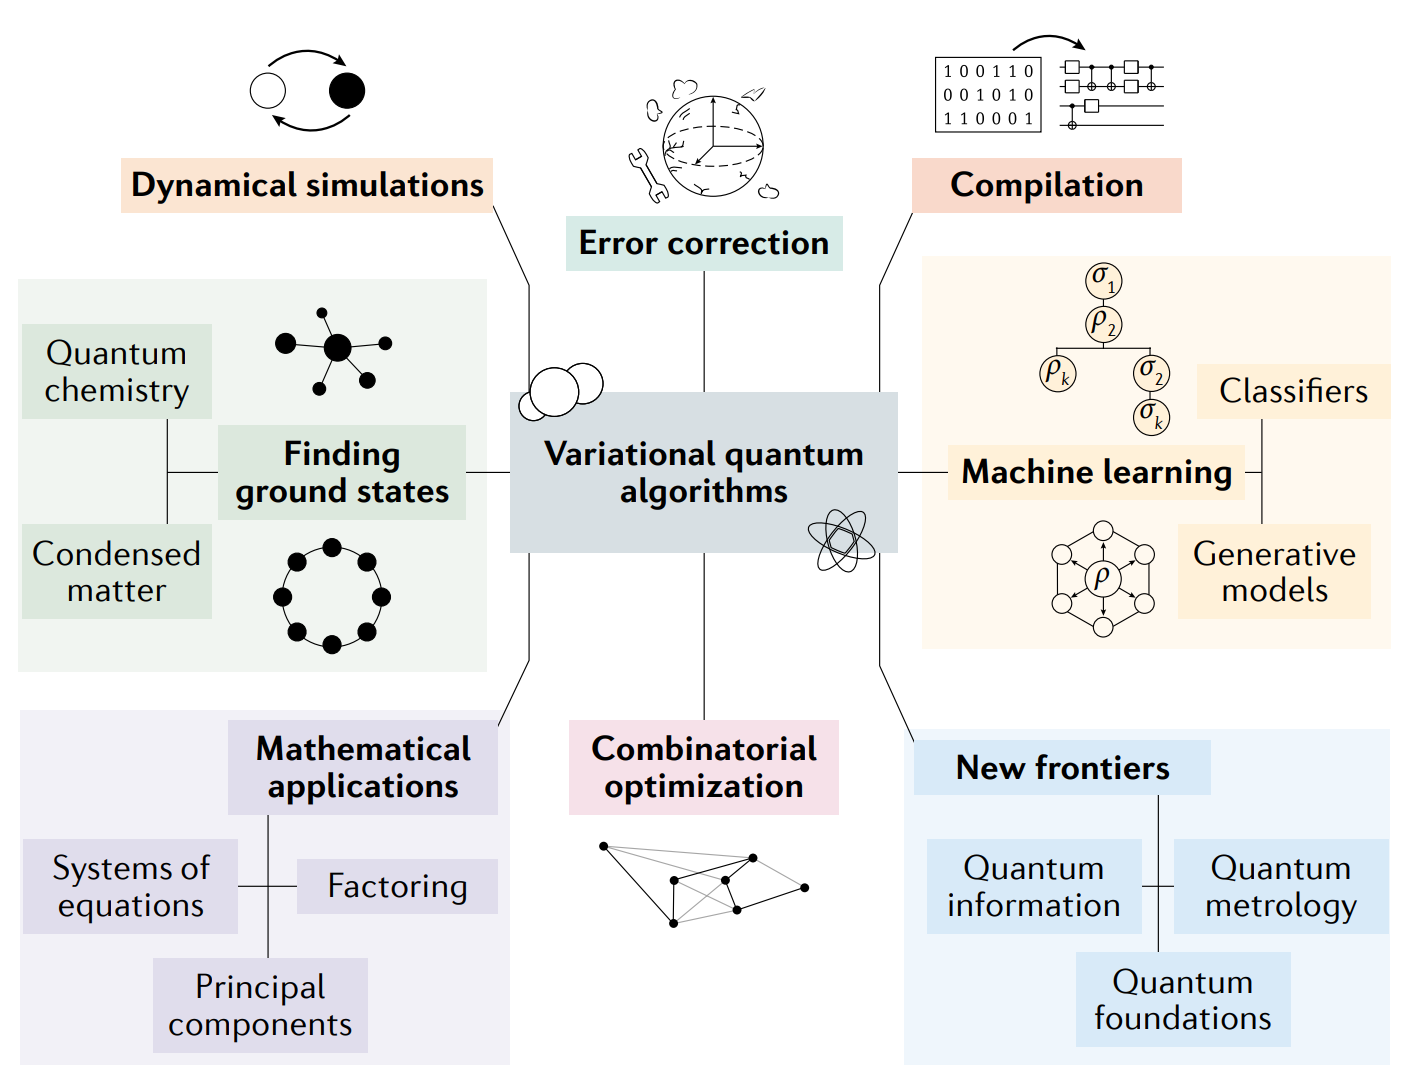
\includegraphics[width=0.65\textwidth]{Figures/Diagrams/VQAs_Applications.png}
  \caption{Applications of variational quantum algorithms. Sourced from \cite{Cerezo_2021} in its entirety.}
  \label{fig:VQAs_Applications}
\end{figure}

\begin{figure}[H]
  \centering
  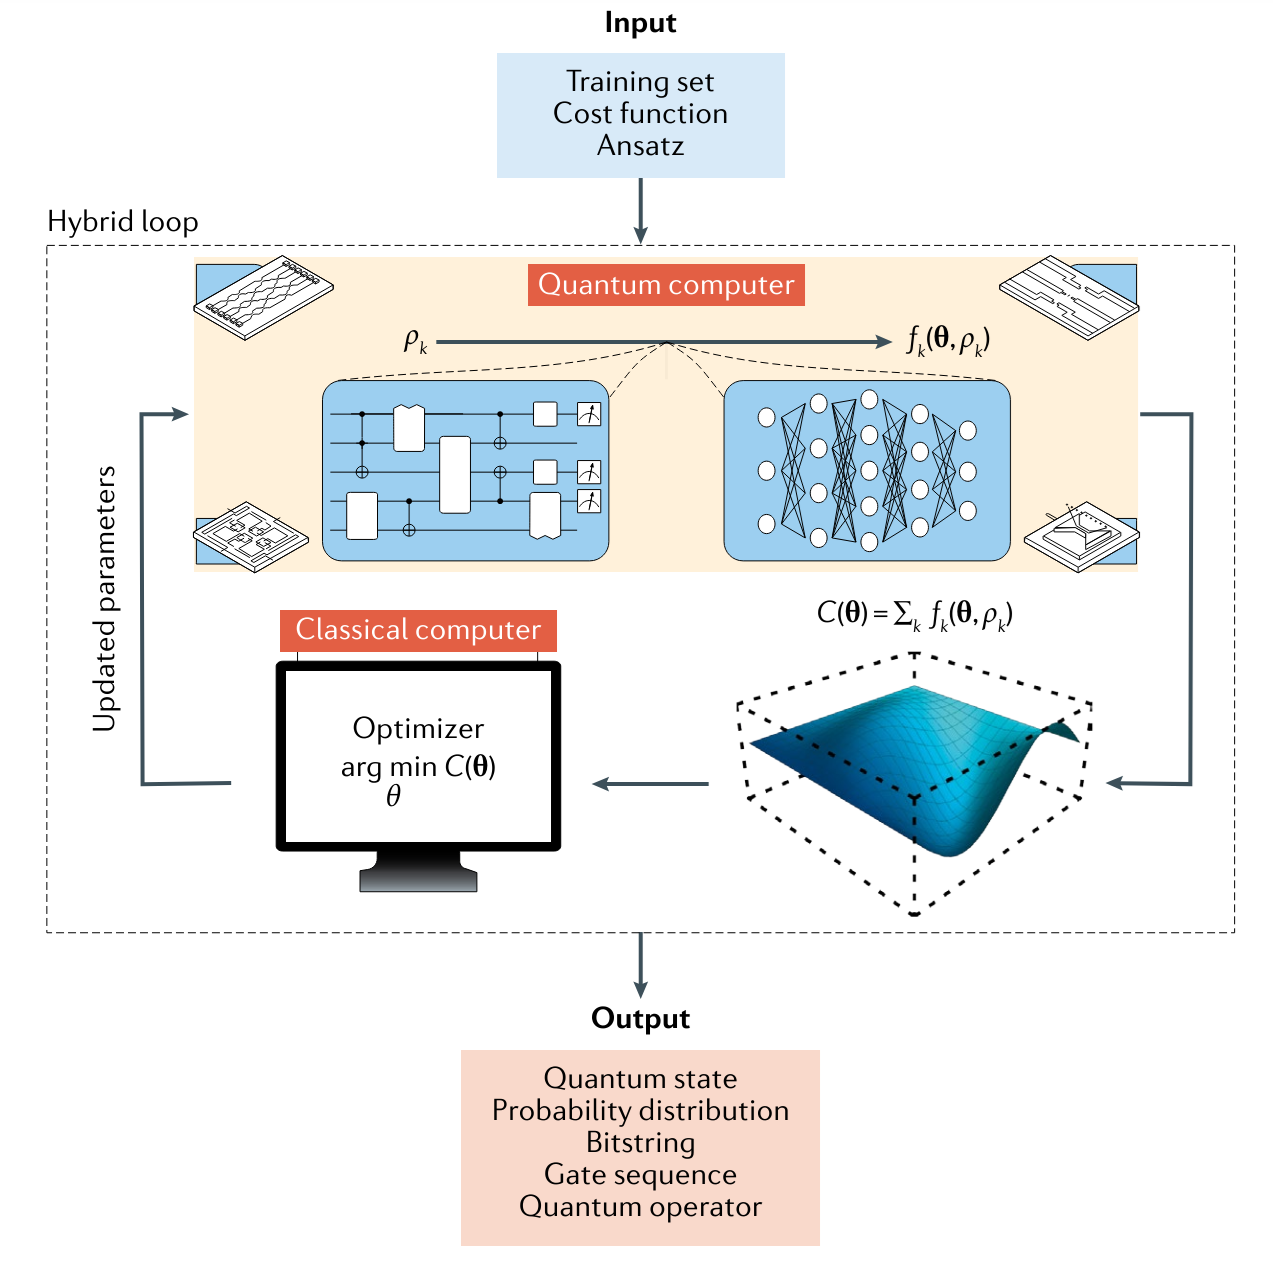
\includegraphics[width=0.65\textwidth]{Figures/Diagrams/VQA_Schematic.png}
  \caption{Schematic diagram of a variational quantum algorithm. Adapted from \cite{Cerezo_2021}.}
  \label{fig:VQA_Schematic}
\end{figure}

% I should re-read EVERYTHING to see if there aren't many repetitions from previously mentioned things.

\subsubsection{Basic structure of a VQA}
\vspace*{-5mm}{\scriptsize \noindent (This description is heavily inspired by \cite{Cerezo_2021}.)}

This section provides an overview of the essential components of \acrshort{vqa}\textcolor{gray}{s}. Kicking off the development of a \acrshort{vqa} involves defining a cost (or loss) function, $C$, that encodes the solution to the problem. Following this, an ansatz is suggested, that is a quantum operation that relies on a set of continuous or discrete parameters, $\boldsymbol{\theta}$, subject to optimization. In other words, we propose the functional form/structure of the parameterized quantum circuit. Afterwards, the suggested ansatz undergoes training, within a hybrid quantum-classical loop (cf. Figure \ref{fig:VQA_Schematic}), to address the following optimization task
\begin{equation}\label{eq:Optimization}
  \boldsymbol{\theta}^{\star} = \arg \min_{\boldsymbol{\theta}} C(\boldsymbol{\theta}),
\end{equation}
corresponding to the minimization of the selected cost function. The distinctive feature of \acrshort{vqa}\textcolor{gray}{s} is their application of a quantum computer to estimate the cost function, $C(\boldsymbol{\theta})$, and its gradient, while relying on classical routines for the optimization of the parameters' values, $\boldsymbol{\theta}$. Next, we provide supplementary information for each step of the \acrshort{vqa} framework.

% Kind of a subsubsubsection.
\subsubsection*{\small Cost function}
An essential aspect of \acrshort{vqa} involves encoding the problem into an adequate cost function. Similar to classical machine learning, this function associates values of the trainable parameters, $\boldsymbol{\theta}$, with real numbers. At a more abstract level, the cost function defines a hypersurface, often termed the cost landscape (cf. Figure \ref{fig:VQA_Schematic}), in a way such that the optimizer's task is to then navigate across this landscape and discover its global minimum, as this would correspond to the sought-after solution. In many instances, it is beneficial and feasible to express the cost in the form:
\begin{equation}\label{eq:Cost}
    C(\boldsymbol{\theta}) = \sum_k f_k\left( Tr\left[O_k U(\boldsymbol{\theta}) \rho_k U^{\dagger}(\boldsymbol{\theta})\right] \right),
\end{equation}
for some set of functions $\{f_k\}$, where $U(\boldsymbol{\theta})$ is a parameterized unitary, $\boldsymbol{\theta}$ is composed of discrete and continuous parameters, $\rho_k$ are input states from a training set and $O_k$ are a set of observables. Note how the argument of $f_k$, $Tr\left[O_k U(\boldsymbol{\theta}) \rho_k U^{\dagger}(\boldsymbol{\theta})\right]$, corresponds to the expectation value of observable $O_k$, in state $\rho_k' = U(\boldsymbol{\theta}) \rho_k U^{\dagger}(\boldsymbol{\theta})$. Oftentimes, it is convenient to design the cost function to be given by the expectation value of a Hamiltonian (e.g., the problem Hamiltonian in \acrshort{qaoa}), which is why we mention that it is beneficial for it to have this specific form. Then, the minimization of the cost corresponds, unambiguously, to the determination of the ground-state energy. Additionally, one frequently uses Pauli operators, whose expectation values are rather easy to compute in practice.

Furthermore, when designing a cost function, we want it to be as faithful as possible, in the sense that its minimum should closely correspond to the desired solution. Likewise, it is imperative that we can efficiently estimate $C(\boldsymbol{\theta})$, as this is integral to the functionality of this method. So far, we have been taking this for granted. However, one must guarantee that this is indeed verified experimentally, otherwise we are not able to proceed.

% Kind of a subsubsubsection.
\subsubsection*{\small Ansätze}
Another crucial element of a \acrshort{vqa} is the ansatz. In broad terms, the ansatz's structure determines the nature of the parameters $\boldsymbol{\theta}$ and, consequently, how they can be optimized to minimize the cost. The design of an ansatz often relies on the specific requirements of the task, allowing for the creation of problem-inspired Ansätze. However, certain ansatz architectures are generic and problem-agnostic, making them applicable even in scenarios where relevant information is lacking. As one might expect, problem-agnostic Ansätze, being more general, will also, usually, require a greater number of parameters, which unsurprisingly hinders the optimization task. However, this also grants them more flexibility. On the other hand, problem-oriented Ansätze are capable of assimilating problem-specific information into the structure of quantum circuits. This custom-fit approach can result in a reduction of the parameter space, making optimization more efficient, and lead to solutions that are more meaningful and interpretable. Furthermore, adopting such an approach might (at times, not always!) enable the use of shallower quantum circuits, thereby aiding in the reduction of overall noise levels. (Greater circuit depths require more quantum gates, which results in more noise.) When it all comes down to it, one should weigh the trade-off between accuracy and generality, and carefully assess resource utilization in the choice of ansatz. (Yet, for achieving optimal results tailored to a specific problem, it's always recommended to utilize problem-inspired Ansätze. The challenge lies in their design. While it's tempting to opt for a problem-agnostic ansatz and consider the task done, problem-inspired designs consistently yield superior performance.) For illustration purposes, here are a few examples of commonly considered ansatz types: hardware-efficient Ansätze (aimed at reducing circuit depth), unitary coupled clustered Ansätze (for quantum chemistry simulations), quantum alternating operator Ansätze (used in \acrshort{qaoa}), \textit{et cetera}.

% Kind of a subsubsubsection.
\subsubsection*{\small Gradients}
After specifying the cost function and ansatz, the next step involves training the parameters, $\boldsymbol{\theta}$, and tackling the optimization problem described in Eq. (\ref{eq:Optimization}). It is known that, for numerous optimization tasks, leveraging information from the gradient or higher-order derivatives of the cost function can enhance the speed and ensure the convergence of the optimizer. A notable benefit of various \acrshort{vqa}\textcolor{gray}{s} is the ability to analytically compute the gradient of the cost function. This can be done using the parameter-shift rule. If the cost function has the form of Eq. (\ref{eq:Cost}), with $f_k(x) = x$, and $\theta_l$ is the $l^{th}$ element in $\boldsymbol{\theta}$, which parameterizes a unitary $e^{i\theta_l \sigma_l}$, with $\sigma_l$ a Pauli operator, then the parameter-shift rule states that the equality
\begin{equation}
    \frac{\partial C}{\partial \theta_l} = \sum_k \frac{1}{2\sin{\alpha}}\left(Tr\left[O_k U(\boldsymbol{\theta_+}) \rho_k U^{\dagger}(\boldsymbol{\theta_+})\right] - Tr\left[O_k U(\boldsymbol{\theta_-}) \rho_k U^{\dagger}(\boldsymbol{\theta_-})\right]\right),
\end{equation}
with $\boldsymbol{\theta_{\pm}} = \boldsymbol{\theta} \pm \alpha \boldsymbol{e_l}$, holds for any real number $\alpha$. In practice, one uses $\alpha = \pi/4$, since this maximizes the accuracy of the result \cite{Cerezo_2021}. Note that, although the expression is analytically exact, we can only ever obtain approximate results (hence the discussion about accuracy), since we are required to compute expectation values of $O_k$, necessitating the quantum circuit to be sampled. This section was simply meant to shed some light on how one can experimentally compute these gradients, required for the optimization procedure.

% Kind of a subsubsubsection.
\subsubsection*{\small Workflow (Hybrid Loop)}
The \acrshort{vqa} workflow is incredibly similar to a traditional machine learning pipeline. We have some input quantum state entering our ansatz, which is then processed by the quantum circuit, parameterized by $\boldsymbol{\theta}$. Afterwards, the output of this circuit is measured and the results are used to compute the cost function, $C(\boldsymbol{\theta})$. Following this, said cost is fed into a classical optimizer, which updates the parameters, $\boldsymbol{\theta}$, in order to minimize the cost\footnote{It's a bit more complex, as we are required to compute the gradients for the classical optimization. For this, we simply use the parameter-shift rule. This requires some more shots, with different parameter values, but is entirely feasible.}. This process [run quantum circuit, estimate cost, update parameters] is repeated iteratively until the optimizer converges to a minimum, at which point the optimal parameters, $\boldsymbol{\theta}^{\star}$, are obtained. These can then be used to prepare the quantum state that solves the problem at hand, in the sense that the problem's solution can be extracted from it. This is a very high-level overview of the \acrshort{vqa} workflow, but it should give a good idea of how the previously mentioned concepts come together to form a working algorithm. All the \acrshort{vqa}\textcolor{gray}{s} described in this work will use this hybrid loop (cf. Figure \ref{fig:VQA_Schematic}). Therefore, specifying the cost function and ansatz will be sufficient to characterize them.

% Kind of a subsubsubsection.
\subsubsection*{\small Applications \& Examples}
In what follows, I will merely outline some of the most promising applications of \acrshort{vqa}\textcolor{gray}{s} for solving real world problems. These are (cf. Figure \ref{fig:VQAs_Applications}): (Specific algorithms for these tasks are indicated in parenthesis.)
\begin{enumerate}
    \item \textbf{Finding ground states and excited states} (Variational Quantum Eigensolver \cite{Peruzzo_2014}, \acrshort{vqe}, and variations thereof);
    \item  \textbf{Dynamical quantum simulations} - Based on iterative variational algorithms, they allow, e.g., for the simulation of open quantum systems \cite{Cerezo_2021};
    \item \textbf{Optimization tasks} (Quantum Approximate Optimization Algorithm \cite{farhi2014quantum}, \acrshort{qaoa}, and Qubit Efficient MaxCut Heuristic Algorithm \cite{tenecohen2023variational}, \acrshort{qemc}, both of which we shall analyse in further detail later);
    \item \textbf{Mathematical applications} \cite{Cerezo_2021} - Linear systems, matrix-vector multiplication, non-linear equations, factoring, \textit{et cetera};
    \item \textbf{Error correction} (Variational Quantum Error Corrector \cite{johnson2017qvector}, QVECTOR);
    \item \textbf{Machine learning and data science} - Quantum Machine Learning (\acrshort{qml}) \cite{Cerezo2022_QML}, classifiers, generative models, \textit{et cetera}.
\end{enumerate}

We are, now, finally ready to tackle the two specific variational quantum algorithms, \acrshort{qaoa} and \acrshort{qemc}, which constitute the main focus of this work. Let us start with \acrshort{qaoa}.

%%%%%%%%%%%%%%%%%%%%%%%%%%%%%%%%%%%%%%%%%%%%%%%%%%%%%%%%%%%%%%%%%%%%%%%%
\subsubsection{Quantum Approximate Optimization Algorithm (QAOA)}
\label{subsubsection:QAOA}

% Include/remove "Review"?

% Describe QAOA - Explain how it works, its advantages and disadvantages, and its potential applications.

% There's a mistake in eq. (5), in the PIC2 report, that I should correct, once I include it here. (It's the coefficients $\gamma$ and $\beta$!) Done!

% I should also change the labels of the problem and mixer Hamiltonians, so they always match the figures. (Sometimes, it's $H_P$ and $H_M$, sometimes it's $H_C$ and $H_B$.) Done!

% Also, mention that $\ket{\psi_0}$ is the uniform superposition state, and that it's the initial state entering the ansatz. Done!

% Specify that $U_{H_{P_l}} = \exp{-iH_P\gamma_l}$. Or something like that. Done!

% I also feel like I don't mention that we use a number of qubits equal to the number of nodes. I should do that. And, then, explain how to interpret the results. (0 - One partition; 1 - The other partition.) Done!

% I should present an explicit (with the actual CNOTs) QAOA ansatz, maybe for the usual $8$-node graph. Or, for the smaller, trivial $4$-node graph. This elucidates the idea of the ansatz. This would also require me to explain how $\exp{-i\gamma Z_i Z_j}$ is transpiled/represented as a quantum circuit. (Look at Bence's TeX file: there's an example there, for $\exp{-i\gamma Z_i Z_j Z_k Z_l}$, I believe.) I think I can present this in the "Implementation" part.

Renowned as the most prominent \acrshort{vqa} in quantum-enhanced optimization, the \acrshort{qaoa} \cite{farhi2014quantum} was originally devised to approximate solutions for combinatorial optimization problems, including constraint-satisfaction, \acrshort{sat} \cite{lin2016performance}, and Max-Cut problems \cite{PhysRevA.97.022304}. In this section, we intend to explain in greater detail the inner workings of \acrshort{qaoa}, since it is closely related to the new hybrid algorithm proposed by the \acrshort{hqcc} project collaboration\footnote{More information about this collaboration is present in the \nameref{sec:acknowledgments} section.}. In a similar vein, the next section will delve into an equivalent level of detail, this time concentrating on the Qubit Efficient MaxCut Heuristic Algorithm, \acrshort{qemc}.

Combinatorial optimization problems are formulated on binary strings, $s = (s_1,...,s_N)$, with the goal of minimizing/maximizing a designated classical objective function, $L(s)$. In \acrshort{qaoa}, however, the cost function is defined as the expectation value of a quantum Hamiltonian, $H_C$ (or $H_P$), termed the cost (or problem) Hamiltonian, and doesn't explictly depend on such bit-string $s$. This [cost] is constructed by mapping each classical variable, $s_j \in \{1, -1\}$, to a Pauli spin-$1/2$ operator, $\boldsymbol{Z}_j$. Thus, the usual MaxCut objective $L(s) = \frac{1}{2}\sum_{\mathrm{Edge}\;(\mathrm{j,k})}(1-s_{i}s_{j})$, denoting the cut of partition $s = (s_1,...,s_N)$, is transformed into the cost Hamiltonian
\begin{equation}\label{eq:H_C}
  H_C = \frac{1}{2}\sum_{\mathrm{Edge}\;(\mathrm{j,k})}(1-\boldsymbol{Z}_i\boldsymbol{Z}_j),
\end{equation}
from which one can extract the \acrshort{qaoa} objective function.

Next up is the \acrshort{qaoa} ansatz. Drawing inspiration from the quantum adiabatic algorithm, \acrshort{qaoa} substitutes adiabatic evolution with $p$ cycles of alternating time evolution between the cost Hamiltonian, $H_C$, and a suitably chosen mixer (or bias) Hamiltonian, $H_M$ (or $H_B$). The role of this mixer Hamiltonian can be understood as introducing quantum fluctuations, or transitions, between different states, helping the algorithm explore the solution space more effectively, ideally preventing it from getting trapped in sub-optimal local minima/maxima. The entirety of this process forms the previously mentioned quantum alternating operator ansatz.

In practice, defining $\boldsymbol{\theta} = \{\boldsymbol{\gamma}, \boldsymbol{\alpha}\}$, the cost function is $C(\boldsymbol{\gamma}, \boldsymbol{\alpha}) = \bra{\psi_p(\boldsymbol{\gamma}, \boldsymbol{\alpha})}H_C\ket{\psi_p(\boldsymbol{\gamma}, \boldsymbol{\alpha})}$, with
\begin{equation}\label{eq:Psi_p}
    \ket{\psi_p(\boldsymbol{\gamma}, \boldsymbol{\alpha})} = e^{-i\alpha_pH_M}e^{-i\gamma_pH_C} ... e^{-i\alpha_1H_M}e^{-i\gamma_1H_C}\ket{\psi_0},
\end{equation}
where $\ket{\psi_0}$ is the initial state entering the ansatz. This ansatz is illustrated in Figure \ref{fig:QAOA_Trotterization}, below, for $n \in \mathbb{N}$ \acrshort{qaoa} layers.
\begin{figure}[H]
    \centering
    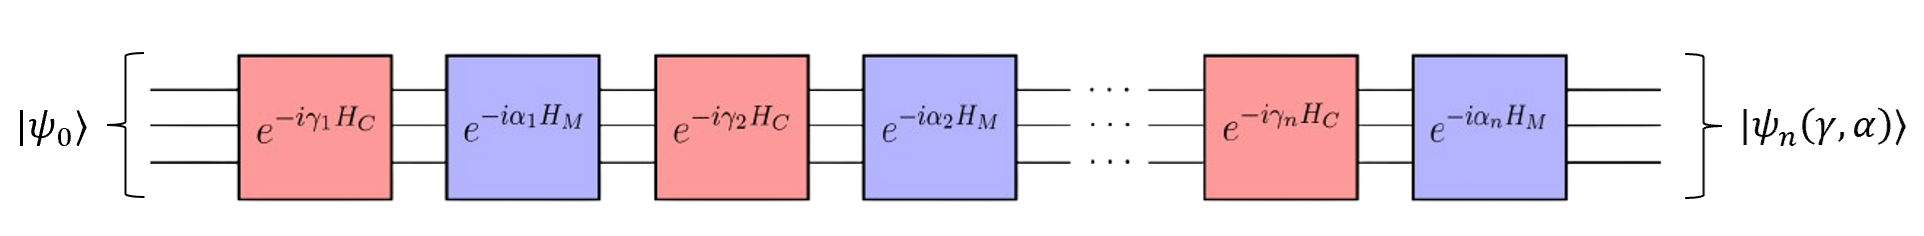
\includegraphics[width = \linewidth]{Figures/Diagrams/QAOA_Trotterization.png}
    \caption{Quantum alternating operator ansatz. Adapted from \cite{Intro_QAOA}.}
    \label{fig:QAOA_Trotterization}
\end{figure}
\noindent Replacing adiabatic time evolution with a \textit{Trotterized} evolution works due to the famous Trotter-Suzuki formulas \cite{nielsen2010quantum}, which state that (for general non-commuting $H_j$):
\begin{equation}
    e^{-i\sum_{j=1}^{m}H_{j}t}=\prod_{j=1}^{m}e^{-i H_{j}t}+O(m^{2}t^{2}).
\end{equation}
If $t \ll 1$, then the error in this approximation becomes negligible. On the other hand, if $t$ is large, Trotter-Suzuki formulas can still be used to simulate the dynamics accurately by breaking things up into a sequence of short time-steps. Let $r$ be the number of steps taken in the time evolution, so each time-step runs for time $t/r$. Then, we have that
\begin{equation}
    e^{-i\sum_{j=1}^{m}H_{j}t}=\left(\prod_{j=1}^{m}e^{-i H_{j}t/r}\right)^{r}+O(m^{2}t^{2}/r),
\end{equation}
which implies that if $r$ scales as $m^2t^2/\epsilon$, then the error can be made at most $\epsilon$ for any $\epsilon > 0$. In the \acrshort{qaoa} case, we simply have $H = H_C + H_M$ and we treat each of the evolution time intervals as variational parameters that are optimized classically (can be seen as $t/r \equiv \gamma_l, \alpha_l$). This means we do not use this \textit{Trotterization} approach directly, but it heavily inspires the \acrshort{qaoa} ansatz nevertheless. 

Let me now further detail the practical realization of the algorithm. Reiterating, the aim of MaxCut is to maximize the number of edges in a graph that are "cut" by a given partition of the vertices into two sets (cf. Figure \ref{fig:MaxCut}). One way of implementing \acrshort{qaoa} for MaxCut is to consider: $H_C$ as in Eq. \ref{eq:H_C}, where the sum is over all edges of the studied graph, connecting vertices $(j, k)$; and $H_M = \sum_{j=1}^{N} \boldsymbol{X_j}$, for $N$ qubits. In this scheme, the associated cost function, $\bra{\psi_p(\boldsymbol{\gamma}, \boldsymbol{\alpha})}H_C\ket{\psi_p(\boldsymbol{\gamma}, \boldsymbol{\alpha})}$, merely rewards cases where we have edges between nodes of different sets. Furthermore, we can, now, also write
\begin{align}
    U_{H_{C_l}} = e^{-i\gamma_l H_C} = \prod&_{\mathrm{Edge}\;(\mathrm{j,k})}e^{-i\gamma_l(1-\boldsymbol{Z}_{j}\boldsymbol{Z}_{k})/2} \\
    U_{H_{M_l}} = e^{-i\alpha_l H_M} = \prod&_{j=1}^{n}e^{-i\alpha_l\boldsymbol{X}_{j}}
\end{align}
These give us the form of the unitaries that are applied in each layer of the \acrshort{qaoa} ansatz, representing the \textit{Trotterized} time evolution of Figure \ref{fig:QAOA_Trotterization} (red and blue boxes). They correspond to the complex exponentials of the cost and mixer Hamiltonians, respectively: $e^{-i\gamma_l H_C}$ and $e^{-i\alpha_l H_M}$. Notice how $U_{H_{M_l}}$ uses Pauli-$x$ operators, instead of the usual Pauli-$z$ in $U_{H_{C_l}}$. In practice, the mixer Hamiltonian terms $e^{-i\alpha_l H_M}$ correspond to $R_x(\alpha_l/2)$ and are easy to implement. The cost Hamiltonian terms, on the other hand, are a bit more tricky, requiring the use of $2$ CNOT gates. Each of the terms $e^{-i\gamma_l(1-\boldsymbol{Z}_{j}\boldsymbol{Z}_{k})/2}$ can be transpiled into a quantum circuit, as shown in Figure \ref{fig:Z_iZ_jDecomposition}, below. For each edge in the graph, we'll have one of these terms, in each of the $p$ layers of the \acrshort{qaoa} ansatz.
\begin{figure}[H]
  \centering
  \begin{quantikz}
  \lstick{Qubit $i$} & \ctrl{1} & \qw                & \ctrl{1}  & \qw & \\
  \lstick{Qubit $j$} & \targ{}  & \gate{R_z(\gamma_l)} & \targ{}   & \qw & \\
  \end{quantikz}
  \caption{$e^{i\gamma_l \boldsymbol{Z}_{i} \boldsymbol{Z}_{j} /2}$ decomposition.}\label{fig:Z_iZ_jDecomposition}
\end{figure}
\noindent This allows us to re-write Eq. \ref{eq:Psi_p} as
\begin{equation}
     \ket{\psi_p(\boldsymbol{\gamma}, \boldsymbol{\alpha})} = U_{H_{M_p}}U_{H_{C_p}} ... U_{H_{M_1}}U_{H_{C_1}}\ket{\psi_0}
\end{equation}
In \acrshort{qaoa}, it is customary to start with a uniform superposition over the $n$ bit-string basis states, i.e., $\ket{\psi_0} = \ket{+_{n}}=\frac{1}{\sqrt{2^{n}}}\sum_{z\in\{0,1\}^{n}}\ket{z}$. This is achieved by applying a Hadamard gate to each of the qubits, at the start of the quantum circuit.

Subsequently, a classical routine is employed to optimize the values of the parameters by minimizing the negative of the cost (analogous to the cut), therefore enabling the extraction of the MaxCut partition. Experimentally, for each step of the classical optimization, it is necessary to compute expectation values of Pauli-$z$ operators, which requires the quantum circuit to be sampled a certain number of times (shots). Additionally, in case it was not yet clear, note that in \acrshort{qaoa} we use one qubit for each node of the graph, with the qubits' values indicating which set they correspond to: $\ket{0}$: "Set 0"; $\ket{1}$: "Set 1". As such, for the graph in Figure \ref{fig:MaxCut}, we'd require $5$ qubits. Exemplifying, if the most sampled basis state at the end of the quantum circuit is $\ket{00011}$, then nodes $1$, $2$ and $3$ belong to "Set 0", while nodes $4$ and $5$ belong to "Set 1".

% I think I should include the "sample simulations" in the "Implementations" section, not here.

%%%%%%%%%%%%%%%%%%%%%%%%%%%%%%%%%%%%%%%%%%%%%%%%%%%%%%%%%%%%%%%%%%%%%%%%
\subsubsection{Variational Qubit-Efficient MaxCut Heuristic Algorithm (QEMC)}
\label{subsubsection:QEMC}

% Re-read all of this!

The Qubit Efficient MaxCut Heuristic Algorithm (\acrshort{qemc}) \cite{tenecohen2023variational} is somewhat similar to \acrshort{qaoa}. After all, it was heavily inspired by it. However, it has a number of crucial differences. First, it only requires $n = \log_2(N)$ qubits, instead of $N$, where $N$ is the number of nodes in the graph. Additionally, the \acrshort{qemc} algorithm is based on a novel probability threshold encoding scheme, a suitable cost function, and a parameterized unconstrained quantum circuit. Going in order:

% Kind of a subsubsubsection.
\subsubsection*{\small Probability threshold encoding scheme}
With $n$ qubits, each of the $N = 2^{n}$ basis states will represent one of the graph's nodes. Following the sampling of the quantum circuit, a probability distribution is generated. Nodes with probabilities exceeding a certain threshold, $p_{th} = \frac{1}{2B}$, belong to "Set 1", while probabilities below this value indicate inclusion in "Set 0". This strongly diverges from how we encode set inclusion in \acrshort{qaoa}.

% Kind of a subsubsubsection.
\subsubsection*{\small Suitable cost function}
The objective function utilized in QEMC is the following:
\begin{equation}
L(\{p(i)\}) = \sum_{\stackrel{j < k:}{\{j,k\}\in E}}\left[\left(d(j,k)-\frac{1}{B}\right)^{2}+\left(s(j,k)-\frac{1}{B}\right)^{2}\right],
\end{equation}
where $d(j,k) = |p(j) - p(k)|$ and $s(j, k) = p(j) + p(k)$ are the absolute difference and sum of the corresponding states' probabilities. The idea is that as both $d(j, k)$ and $s(j, k)$ tend towards $1/B$, the probability of one node approaches zero (distinctive "Set 0"), while the probability of the other node approaches $1/B$ (distinctive "Set 1"), without specifying which is which. Ultimately, just like for \acrshort{qaoa}, connections between nodes of different sets are favoured. Note, however, that this probability threshold encoding scheme assumes, \textit{a priori}, that one of the sets ("Set 1") has $B$ nodes. Nevertheless, this is not an issue, as we can efficiently iterate through all potential values of $B\,=\,1,...,\left\lfloor{\frac{N}{2}}\right\rfloor$. Frequently, it is reasonable to set $B = N/2$, and we shall use this as our starting point.

% Kind of a subsubsubsection.
\subsubsection*{\small Problem-agnostic quantum circuit}
The \acrshort{qemc} circuit ansatz is agnostic to specific graph instances, a departure from \acrshort{qaoa} where the graph structure is explicitly encoded in the quantum circuit. Instead, the graph is implicitly encoded through the cost function. As a result, the \acrshort{qemc} quantum circuit is not bound to any particular form and only needs to be expressive enough to approximate the optimal states in the Hilbert space. Such problem-independent ansatz approach provides considerable flexibility in ansatz selection. Frequently, the circuit ansatz known as "Strongly Entangling Layers" is employed, as depicted below (Figure \ref{fig:Strongly_Entangling_Layers}). As can be seen, this ansatz applies a series of parameterized single-qubit rotations interspersed with controlled entangling gates to generate a highly entangled quantum state. We use Pennylane's \href{https://docs.pennylane.ai/en/stable/code/api/pennylane.StronglyEntanglingLayers.html}{\texttt{qml.StronglyEntanglingLayers}} implementation for this purpose.

\begin{figure}[H]
    \centering
    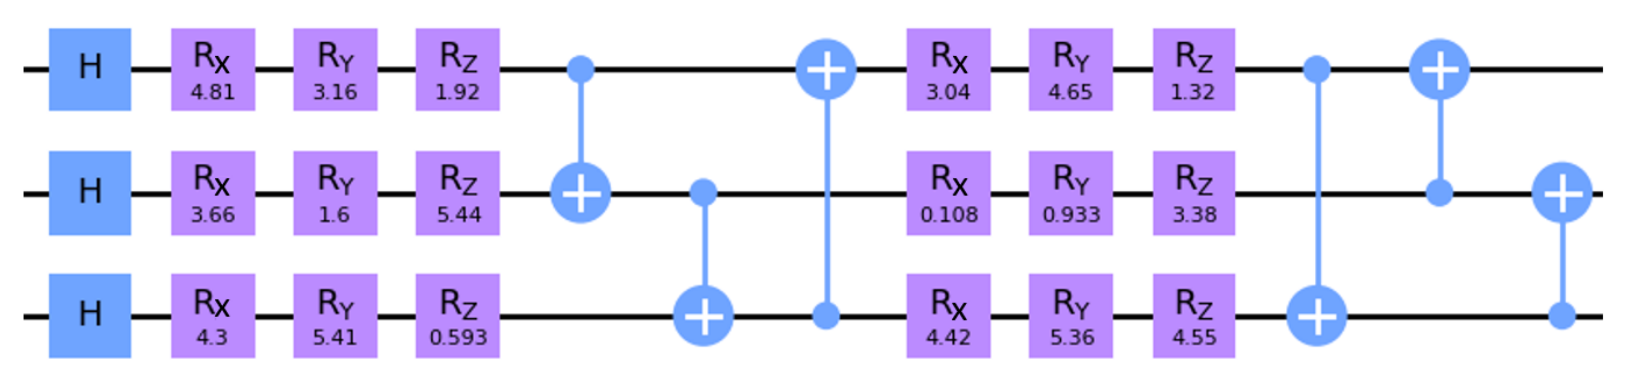
\includegraphics[width = 0.85\linewidth]{Figures/Diagrams/Strongly_Entangling_Layers.png}
    \caption{"Strongly Entangling Layers" circuit ansatz: case of $n = 3$ qubits and $p = 2$ layers. After a single layer of Hadamard gates, each subsequent layer consists of $3n$ single-qubit parameterized rotation gates and $n$ CNOT gates (entangling gates). Reproduced from \cite{tenecohen2023variational}.}
    \label{fig:Strongly_Entangling_Layers}
\end{figure}

These constitute the main ingredients necessary to understand the \acrshort{qemc} algorithm. At this point, the same hybrid loop as before would be run, so as to optimize the "Strongly Entangling Layers" ansatz's parameters, to minimize the cost function. To read the MaxCut partition, generated by the \acrshort{qemc} algorithm, one would sample the circuit's output one more time, after the training, and build the basis states' probabilities distribution. The threshold $p_{th}$ would then be applied to determine each nodes' set inclusion, from each of their associated basis states' probabilities.

One notable, and perhaps unfortunate, property of \acrshort{qemc} is that it is efficiently simulable classically. Due to the exponential compression of the number of qubits, the algorithm can be feasibly run on a classical computer, even for large graphs, hence defeating its purpose as a quantum algorithm. This is something the authors of the algorithm \cite{tenecohen2023variational} realized in hindsight. For this reason, it is now termed a quantum-inspired classical algorithm.

% I'm missing the "Implementation" part, here. Also, re-read all of this!

% Include/remove "Review"?

% Describe QEMC - Explain how it works, its advantages and disadvantages, and its potential applications.

% The reason why we can efficiently iterate through the values of $B$ is that we have a reduced number of qubits (exponential compression). [I think so, at least.] We always say the set with $B$ blue nodes is the smallest. Aka., $B \leq N/2$, where $N$ is the graph's number of nodes.

% Is there any reason for this, though? What would happen if we said $B > N/2$? (Aka., the blue set is the one with the most nodes.)

% Mention that the problem-agnostic "Strongly-Entangling-Layers" ansatz might result in "too much entanglement", thus hindering the results.

% Go over the last paragraph of the QEMC section again. Something about the discussion on "shot number" is bugging me. % file "Thesis_Background.tex"
\cleardoublepage

%%%%%%%%%%%%%%%%%%%%%%%%%%%%%%%%%%%%%%%%%%%%%%%%%%%%%%%%%%%%%%%%%%%%%%%%
%                                                                      %
%     File: Thesis_Base_Algorithm.tex                                      %
%     Tex Master: Thesis.tex                                           %
%                                                                      %
%     Author: Andre C. Marta                                           %
%     Last modified :  4 Mar 2024                                      %
%                                                                      %
%%%%%%%%%%%%%%%%%%%%%%%%%%%%%%%%%%%%%%%%%%%%%%%%%%%%%%%%%%%%%%%%%%%%%%%%

\chapter{iQAQE Framework}
\label{chapter:Base Algorithm}

% I should probably re-write this a bit, such that it is obvious what we mean when we say 'iQAQE Framework'. I've said this before, but it needs to appear here, again.

% Something, something, HQCC-project collaboration. I should probably mention this earlier than I do at the moment. (It's just some footnote, right now... I should change this, probably. Although, it is not too important, I guess.)

In this chapter, we present the \acrshort{iqaqe} Framework, which interpolates between \acrshort{qaoa} and \acrshort{qemc}. We begin with a comparison of the two algorithms, followed by a detailed description of \acrshort{iqaqe}, its theoretical model, motivation, and workflow.

% In this chapter, we present the proposed algorithm, \acrshort{iqaqe}, which interpolates between \acrshort{qaoa} and \acrshort{qemc}. We begin with a comparison of the two algorithms, followed by a detailed description of \acrshort{iqaqe}, its theoretical framework, motivation, and workflow.

\section{Comparison of QAOA and QEMC}
To motivate the development of our new algorithm(s), we summarize the merits and drawbacks of both \acrshort{qaoa} and \acrshort{qemc}. \acrshort{qemc} has several advantages over \acrshort{qaoa}, including significantly lower qubit requirements ($n = \log_2(N)$ vs. $N$) and the ability to support shallower circuit depths \cite{tenecohen2023variational}. The threshold probability encoding scheme allows \acrshort{qemc} to associate each graph partition with a volume of quantum states, potentially enhancing noise resilience. Moreover, \acrshort{qemc} might be better trainable \cite{tenecohen2023variational}. However, \acrshort{qemc} requires the entire probability distribution at each optimization step to compute the cost, increasing the number of needed shots compared to \acrshort{qaoa}, which only requires expectation values. Additionally, it has been shown that \acrshort{qemc} can be efficiently simulated classically, somewhat undermining its purpose as a quantum algorithm \cite{tenecohen2023variational}.

Having thoroughly understood these two algorithms, the collaboration within the \acrshort{hqcc} project has introduced a novel framework for designing multiple distinct \acrshort{vqa}\textcolor{gray}{s}. This will be the focus of our next discussion.

% With a thorough grasp of these two algorithms, the \textit{HQCC}-project collaboration has put forward a novel hybrid algorithm that integrates aspects from both, intending to capitalize on their individual strengths for a more substantial outcome. This is what we will be discussing next.

%%%%%%%%%%%%%%%%%%%%%%%%%%%%%%%%%%%%%%%%%%%%%%%%%%%%%%%%%%%%%%%%%%%%%%%%
\section{Interpolated QAOA/QEMC Hybrid Algorithm (iQAQE)}
\label{section:iQAQE}

% I'll keep the cardinality in [1, 2**(n-1)], for n qubits, under the argument that: 1 - QEMC, and 2**(n-1) - QAOA. Later, I might mention that we relax this constraint, allowing for 2**n - 1, as well. That is only towards the end, when I'm doing those bar plots with performance bins, etc. [Many colours, etc.]

\subsection{Theoretical Model}
\label{subsection:iQAQE Theoretical Framework}
Algorithms developed within the proposed framework aim to interpolate between \acrshort{qaoa} and \acrshort{qemc}, combining their strengths into a more robust approach, tentatively named \acrshort{iqaqe} (Interpolated QAOA/QEMC). In \acrshort{iqaqe}, we depart from the \acrshort{qemc} approach by associating each graph node with a list (sometimes also called a sub-list) of basis states, in contrast to \acrshort{qemc}'s consideration of a single basis state for each node (cf. Figure \ref{fig:iQAQE_Encoding}). Each of these lists comprises somewhere between $\left[1, 2^{n-1}\right]$ basis states, where $n$ represents the number of qubits. The number of basis states per list is called the list's cardinality, denoted as $c$. This design allows for potential overlap among states from different lists/nodes. What we formerly referred to as "mapping" involves distributing basis states among these lists. The term "mapping" can also signify a specific allocation of basis states among the lists. Additionally, it is important to note that the encoding of these states will utilize a qubit range expected to fall between the \acrshort{qemc} and \acrshort{qaoa} requirements, specifically in $[\log_2(N), N]$, for an $N$-node graph. With all that said, the main goal of my thesis is to ascertain the optimal mapping from basis states to lists, essentially determining which basis states should be included in specific lists/nodes. Naturally, this undertaking also involves the identification of a suitable cost function and ansatz to ensure the algorithm's effective operation. For most of our work, we consider \acrshort{iqaqe} to use the same ansatz and cost function as \acrshort{qemc}, adjusted for the appropriate number of qubits and with some modifications that we'll discuss below.

% Figure: iQAQE Encoding
\begin{figure}[H]
    \centering
    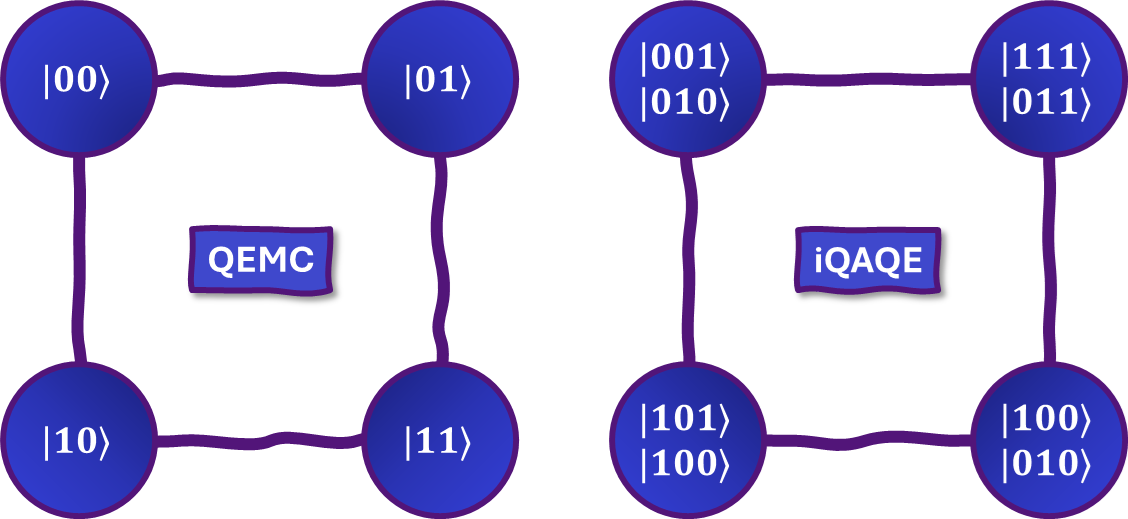
\includegraphics[width=0.8\textwidth]{Figures/Diagrams/QEMC_iQAQE_Encodings.png}
    \caption{Sample schematic representation of the \acrshort{iqaqe} encoding scheme. Comparison between the \acrshort{qemc} and \acrshort{iqaqe} encoding schemes: example for a trivial $4$-node graph. In \acrshort{qemc}, each node is associated with a single basis state, while in \acrshort{iqaqe}, each node is associated with a list of basis states.}
\label{fig:iQAQE_Encoding}
\end{figure}

\subsection{Motivation \& Outlook}
\label{subsection:iQAQE Motivation}
At this point, it is important to mention that the development of this algorithm is entirely exploratory, although we do believe it should allow for a more practical algorithm implementation-wise. We can postulate that such a hybrid approach might have some potential advantages. Namely, it should allow for less shots than in \acrshort{qemc} and fewer qubit requirements than in \acrshort{qaoa}, in addition to, arguably, being better trainable. Another interesting characteristic of such an algorithm is its tunable "quantum-ness". As we interpolate between \acrshort{qaoa} (hybrid quantum-classical) and \acrshort{qemc} (classical, quantum-inspired), the ability to selectively adjust the degree of both could prove to be advantageous. As part of a more long-term perspective (not in this thesis), I may explore the possibility of generalizing this algorithm to tackle additional combinatorial problems, such as Max-$k$-Cut. Throughout my thesis, I will rigorously test the algorithm using classical simulations of quantum machines. The aim is to identify the most effective implementation strategies, taking into account both cost and ansatz considerations, as well as the distribution of basis states.

\subsection{Algorithm Description \& Workflow}
\label{subsection:iQAQE Description_Workflow}
A sketch of the workflow is provided below (Table \ref{tab:iQAQE_Steps}). Regarding the hybrid loop, I only detail the changes relative to \acrshort{qemc}. Following this, I will elaborate on each step.
\begin{table}[h!]
    \centering
    \begin{tabular}{|c|p{9.5cm}|}
    \hline
    \textbf{Step} & \textbf{Description} \\ \hline
    $1.$ \textbf{Select number of qubits} & \texttt{n\_qubits}$ = n \in \left[\log_2{(N)}, N\right]$, where $N$ refers to the graph's number of nodes. \\ \hline
    $2.$ \textbf{Select list cardinality} & \texttt{list\_cardinality}$ = c \in \left[1, 2^{n - 1}\right]$, where $n$ represents the chosen number of qubits. Note that $c$ is taken to be the same for all the nodes, although this could change in future work. \\ \hline
    $3.$ \textbf{Assignment/mapping} & Map $c$ basis states to each graph node. \\ \hline
    \makecell{$4.$ \textbf{Calculate nodes' probabilities} \\ \textbf{(within the hybrid loop)}} & To obtain each node's probability, sum the probabilities of the basis states in the list and normalize the results, so they add up to $1$. \\ \hline
    \makecell{$5.$ \textbf{Cost function and ansatz} \\ \textbf{(within the hybrid loop)}} & Keep the same cost function and ansatz as in the \acrshort{qemc} algorithm, just adapt the ansatz to the correct number of qubits. \\ \hline
    \end{tabular}
    \caption{Core steps for algorithms built on the \acrshort{iqaqe} Framework.}
    \label{tab:iQAQE_Steps}
\end{table}

\subsubsection*{$1.$ Select the number of qubits}
In selecting the number of qubits, we allow for any intermediate value between the \acrshort{qemc} ($\log_2{(N)}$) and \acrshort{qaoa} ($N$) limits. This should give us more flexibility regarding the degree of "quantum-ness" that we want our algorithm to exhibit. This is to be understood in the context of \acrshort{qemc} being entirely classical, whereas \acrshort{qaoa} is hybrid quantum-classical. As such, by choosing a number of qubits in between these two limits, we expect our algorithm to be hybrid in terms of its quantum nature. In addition to this, the number of qubits, alongside the ansatz, will also influence the expressivity of the model.

Another key consideration, closely tied to our next workflow step, is the chosen encoding method. This refers to how we determine each node's color and map basis states to respective lists. Different encoding strategies, such as using expectation values of Pauli strings (e.g., as seen in \cite{sciorilli2024largescale}), inherently influence the number of required qubits. For instance, the Pauli string encoding in \cite{sciorilli2024largescale} automatically enforces a polynomial compression on the number of qubits. Currently, we've employed \acrshort{qemc}'s probability threshold encoding scheme, offering flexibility in deriving node probabilities from basis states. Further discussion on this will be provided in point $4$ below.

\subsubsection*{$2.$ Select list cardinality}
If it hasn't been clear already, we assign a list of basis states to each graph node. The cardinality of each list, denoted as $c$, falls within the interval $\left[1, 2^{n-1}\right]$, where $n$ denotes the number of qubits used. This choice represents a balance between the \acrshort{qemc} ($1$) and \acrshort{qaoa} ($2^{n-1}$) extremes. Determining the optimal value for $c$ is non-trivial, as it depends on various interconnected factors including the number of qubits, ansatz, cost function, and color encoding. To explore its impact on algorithm performance, we conduct grid searches on this parameter.

\subsubsection*{$3.$ Assignments/mapping}
The process of mapping basis states to lists adds significant complexity. \textit{A priori}, there's no clear-cut method for this mapping. The simplest approach involves randomly assigning $c$ basis states to each node, ensuring all states are utilized at least once to avoid discarding information. However, exploring more intricate mappings may yield potential benefits. For instance, in the \acrshort{qaoa} mapping, a single qubit among $N$ is fixed to $1$ for each node, allowing for $2^{N-1}$ permutations of the remaining qubits. In other words, each list, comprising $2^{N-1}$ elements, corresponds to a distinct graph node, with each node having a different qubit fixed to $1$. As can be noted, there's a myriad of distinct mappings one can build, which we'll thoroughly examine in Chapter \ref{chapter:Schemes_and_Results}, each presenting its unique advantages and disadvantages. The challenge lies in identifying the most effective mapping for a given problem instance. We aim to address this in our work.

\subsubsection*{$4.$ Calculate nodes' probabilities}
Above (Table \ref{tab:iQAQE_Steps}), we mentioned a straightforward method of computing node probabilities by summing the probabilities of associated basis states and normalizing the result. This approach serves as our foundational strategy throughout this work. However, there may be hidden advantages in devising more intricate methods. For instance, one could explore calculating node probabilities using the arithmetic or geometric averages of basis states' probabilities, followed by normalization. Yet, designing such schemes requires caution, as mismatches between the ansatz and encoding could result in constant probabilities for nodes, impeding variational circuit optimization\footnote{This occurred once during testing when we used the \acrshort{qaoa} mapping and ansatz alongside the \acrshort{qemc} cost function and probability threshold encoding scheme.}. Furthermore, the normalization process itself may eliminate the probabilities' dependence on variational parameters under certain circumstances. While we explore alternative methods for calculating probabilities, our primary emphasis in this work remains on the basic approach described earlier, given its apparent robustness.

\subsubsection*{$5.$ Cost function and ansatz}
We employ the \acrshort{qemc} cost function, utilizing the probability threshold encoding scheme mentioned earlier. It's important to note that this scheme assumes, by default, that one of the sets ("Set 1") comprises $B$ nodes\footnote{This value is user-defined.}, which may not align with the \acrshort{maxcut} partition. In some cases, we may need to iterate through potential values of $B$, ranging from 1 to $\left\lfloor{\frac{N}{2}}\right\rfloor$ – although, in practice, careful selection of $B$ should prevent this scenario. Often, setting $B = N/2$ proves to be a reasonable starting point, and we adopt this as our default.

Given our approach to mapping basis states to node lists, it's logical for us to employ the \acrshort{qemc} cost function rather than \acrshort{qaoa}'s. The latter relies on a problem Hamiltonian defined on $N$ qubits, which may not match our choice of $n$. Typically, $n < N$ as we aim to reduce the number of qubits. % Removed: ", making $n = N$ impractical."

Similarly, we opt for the Strongly Entangling Layers ansatz from the \acrshort{qemc} scheme for its versatility regarding qubit count. This ansatz, agnostic to specific problems, offers flexibility in our algorithm's implementation compared to \acrshort{qaoa}'s problem-inspired ansatz. However, there are plans to explore more tailored ansatz designs correlated with individual mappings, aiming to enhance algorithm performance by leveraging graph-specific information. Note that this may necessitate an adjusted objective function developed with these considerations in mind. While we experiment with problem-inspired ansätze in this work, our primary focus remains on the Strongly Entangling Layers ansatz.

% One of our goals should've been to reduce the number of shots required. However, as it stands, today, we didn't work through that. We've always been doing analytical simulations... At some point in the future, it'd be interesting to explore this further.

% Tomorrow, 14/05, I should go over all this section! Re-read everything and possibly shorten some of this. There will, for sure, be things that I want to remove/change, e.g.

% Describe iQAQE - Explain how it works, its advantages and disadvantages, and its potential applications. Also, mention how iQAQE has many degrees of freedom that can be tuned, which led to the development of many variations of iQAQE, springing from the original idea. These will be described in the \nameref{chapter:Schemes_and_Results} chapter.

% In the PIC2 report, I sort of contradict myself in the end when I mention that "[...] it is somewhat inefficient to iterate over the possible $B$ values [...]". I should correct this (just remove this sentence).

% Sub-lists' cardinalities interval: $[1, 2^N -1]$. In the PIC2 report, it states $[1, 2^{N -1}]$, which is, indeed, what I used for the simulations. However, there's no reason why we shouldn't be allowed to consider $2^N -1$ maximum number of basis states per list. I should put this disclaimer somewhere in here (Thesis).

% In the "Motivation behind this work" section in the PIC2 report, there's a number of things that need to be re-written, before being included here! Remember to do this! (Inefficient $B$ iterations, better trainability - fewer parameters?, etc.)

% There's also a bit of redundancy in this chapter. % add new .tex files for new chapters
\cleardoublepage

%%%%%%%%%%%%%%%%%%%%%%%%%%%%%%%%%%%%%%%%%%%%%%%%%%%%%%%%%%%%%%%%%%%%%%%%
%                                                                      %
%     File: Thesis_Implementation.tex                                  %
%     Tex Master: Thesis.tex                                           %
%                                                                      %
%     Author: Andre C. Marta                                           %
%     Last modified :  4 Mar 2024                                      %
%                                                                      %
%%%%%%%%%%%%%%%%%%%%%%%%%%%%%%%%%%%%%%%%%%%%%%%%%%%%%%%%%%%%%%%%%%%%%%%%

\chapter{Implementation details}
\label{chapter:implementation}

In this chapter, we outline the numerical implementation of the models discussed in Chapters~\ref{chapter:Background} and \ref{chapter:Base Algorithm}, focusing on pseudo-code representations. Furthermore, we highlight the Python libraries employed and provide specific code details, accompanied by a brief discussion on the benchmarks developed to evaluate the algorithms' performances.

% Pseudo-codes, numerical methods, and benchmarking of the implemented models. Also, put here the basic examples of QAOA and QEMC, I think.

% Insert your chapter material here. - In this chapter, we should describe numerical aspects of the algorithms' implementations. This goes for all three of QAOA, QEMC and iQAQE. Mention Pennylane, the developed code/models, the GitHub repository, and any other relevant information. Mention, also, that we're always doing numerical simulations of quantum systems, on a classical computer!

%%%%%%%%%%%%%%%%%%%%%%%%%%%%%%%%%%%%%%%%%%%%%%%%%%%%%%%%%%%%%%%%%%%%%%%%
\section{Individual Algorithms}
\label{section:Individual_Algorithms}

For numerical implementation of the previously described algorithms, we employ PennyLane \cite{Pennylane}, a versatile Python library designed for differentiable programming of quantum computers. PennyLane facilitates the execution of variational quantum circuits and their simultaneous training, akin to training a classical neural network, within the same Python environment, which is highly convenient. It offers numerous features, including automatic differentiation, crucial for optimizing variational quantum circuits.

In our implementation with PennyLane, we utilize one of two devices from its extensive selection. Firstly, we employ the \texttt{default.qubit} device, a straightforward state-vector qubit simulator implemented in Python, compatible with Autograd, JAX, TensorFlow, and Torch backends. This device is well-suited for optimizations involving a small to moderate number of qubits and parameters, offering exact expectation values. Secondly, we utilize the \texttt{lightning.qubit} device, a fast state-vector qubit simulator with a C++ backend. Recommended for scenarios involving moderate numbers of qubits and parameters or when utilizing stochastic expectation values. Our simulations utilize both devices: the former excels in analytical simulations of small quantum circuits, which predominates our work, while the latter is preferable for numerical simulations of larger quantum circuits, especially when multiple shots are required. Although analytical simulations are favored due to their lower computational resource requirements, they may lack the output sampling aspect of a true quantum computer simulation. Nonetheless, they suffice for our goal of optimizing variational quantum circuit parameters.

Moreover, we heavily rely on the NetworkX \cite{NetworkX} Python library, a valuable tool for creating, manipulating, and analyzing complex networks. NetworkX aids in generating the graphs utilized in the MaxCut problem, offering useful visualization tools for graph representation and partitioning visualization, essential for interpreting algorithm results.

Additionally, we utilize the CVXPY \cite{cvxpy} Python library, specifically designed for convex optimization tasks. CVXPY facilitates solving the semidefinite programming (\acrshort{sdp}) relaxation of the MaxCut problem within the \acrshort{gw} algorithm framework, which inherently constitutes a convex optimization problem.

Regrettably, we lack access to a genuine quantum computer, which would have been invaluable for assessing the performance of these algorithms on real hardware. Furthermore, the lack of access to a High-Performance Computing (\acrshort{hpc}) cluster significantly limited our capacity to perform large-scale simulations and grid-searches necessary for hyperparameter tuning. These limitations occasionally posed a bottleneck in our research, particularly concerning our inability to evaluate the algorithms on larger graphs, which would have been crucial for comprehensive testing. All simulations presented herein were conducted using my personal computer – a system equipped with an 8-core AMD Ryzen 7 5800H CPU, integrated Radeon graphics\footnote{No GPU-assisted computations were conducted.}, and 16GB of RAM.

Lastly, all simulations were performed using the Adam classical optimizer \cite{kingma2017adam}, with default parameters except for the learning rate, which was treated as a hyperparameter and fine-tuned accordingly. The Adam optimizer is a popular optimization algorithm for variational quantum algorithms, utilizing stochastic gradient descent with adaptive learning rates and momentum.

% Description of the numerical implementation of the models explained in Chapter~\ref{chapter:Background}.

% If needed, pseudo-codes can be included as exemplified in Algorithm~\ref{euclid}.
% %
% % See package 'algorithmicx' for more information
% % https://ctan.org/pkg/algorithmicx
% %
% \begin{algorithm}
% \caption{Euclid’s algorithm}\label{euclid}
% \begin{algorithmic}[1]
% \Procedure{Euclid}{$a,b$}\Comment{The g.c.d. of a and b}
%    \State $r\gets a\bmod b$
%    \While{$r\not=0$}\Comment{We have the answer if r is 0}
%       \State $a\gets b$
%       \State $b\gets r$
%       \State $r\gets a\bmod b$
%    \EndWhile\label{euclidendwhile}
%    \State \textbf{return} $b$\Comment{The gcd is b}
% \EndProcedure
% \end{algorithmic}
% \end{algorithm}

%%%%%%%%%%%%%%%%%%%%%%%%%%%%%%%%%%%%%%%%%%%%%%%%%%%%%%%%%%%%%%%%%%%%%%%%
\subsection{Quantum Approximate Optimization Algorithm (QAOA)}
\label{subsection:QAOA_Implementation}

% Description of the numerical implementation of the QAOA model.

Below, we present the pseudo-code representation of the Quantum Approximate Optimization Algorithm (\acrshort{qaoa}) implementation, as described in subsubsection \ref{subsubsection:QAOA}.

\begin{algorithm}[H]
   \small
   \caption{Quantum Approximate Optimization Algorithm (\acrshort{qaoa})}\label{alg:QAOA}
   \begin{algorithmic}
   \Require \texttt{graph}, \texttt{n\_layers}, \texttt{init\_parameters}
   \Ensure \texttt{n\_qubits = graph.n\_nodes}
   \State 1. Define $U_C$ and $U_M$
   \State 2. Create variational circuit using \texttt{@qml.qnode} with $p$ layers of $U_C$ and $U_M$
   \State \hskip1em \textbf{Note:} Start with \texttt{qml.Hadamard} on all qubits
   \State 3. Define objective function: $\langle H_C \rangle$, obtained through \texttt{qml.expval(H\_C)}
   \State 4. Initialize Adam optimizer with default parameters
   \State 5. Start timer \& begin training:
   \While{True}
       \State 5.1 Update \texttt{parameters} using Adam
       \State 5.2 Store cut value, cost function, and approximation ratio, for each iteration
       \If{\texttt{max\_iter} \textbf{or} \texttt{abs\_tol} \textbf{or} \texttt{rel\_tol} reached}
           \State \textbf{break}
       \EndIf
   \EndWhile
   \State 6. Stop timer: record training time
   \State 7. Sample circuit to get most frequent bitstring
   \State 8. Compute partition \& corresponding cut value
   \end{algorithmic}
\end{algorithm}

All of the developed code has been compiled in a GitHub repository, available at \url{https://github.com/kaiuki2000/HQCC_Code_Implementations/tree/main}. For access to the code, please contact the author.

%%%%%%%%%%%%%%%%%%%%%%%%%%%%%%%%%%%%%%%%%%%%%%%%%%%%%%%%%%%%%%%%%%%%%%%%
\subsection{Qubit-Efficient MaxCut Heuristic (QEMC)}
\label{subsection:QEMC_Implementation}

% Description of the numerical implementation of the QEMC model.

Here, we provide the pseudo-code representation of the implementation of the Qubit-Efficient MaxCut Heuristic (\acrshort{qemc}), as detailed in subsubsection \ref{subsubsection:QEMC}.

\begin{algorithm}[H]
   \small
   \caption{Qubit Efficient MaxCut Heuristic Algorithm (\acrshort{qemc})}\label{alg:QEMC}
   \begin{algorithmic}
   \Require \texttt{graph}, \texttt{n\_layers}, \texttt{init\_parameters}, \texttt{B} \Comment{\texttt{B} is a parameter of the cost function}
   \Ensure \texttt{n\_qubits = graph.n\_nodes}
   \State 1. Define \acrshort{qemc} ansatz layer (Strongly Entangling Layers)
   \State 2. Create variational circuit using \texttt{@qml.qnode} with \acrshort{qemc} ansatz
   \State \hskip1em \textbf{Note:} Start with \texttt{qml.Hadamard} on all qubits
   \State 3. Define objective function using probability threshold encoding scheme
   \State 4. Initialize Adam optimizer with default parameters
   \State 5. Start timer \& begin training:
   \While{True}
       \State 5.1 Update \texttt{parameters} using Adam
       \State 5.2 Store cut value, cost function, and approximation ratio, for each iteration
       \If{\texttt{max\_iter} \textbf{or} \texttt{abs\_tol} \textbf{or} \texttt{rel\_tol} reached}
           \State \textbf{break}
       \EndIf
   \EndWhile
   \State 6. Stop timer: record training time
   \State 7. Sample circuit to get output probability distribution
   \State 8. Compute partition using probability threshold encoding scheme \& corresponding cut value
   \end{algorithmic}
\end{algorithm}

%%%%%%%%%%%%%%%%%%%%%%%%%%%%%%%%%%%%%%%%%%%%%%%%%%%%%%%%%%%%%%%%%%%%%%%%
\subsection{Interpolated QAOA/QEMC Hybrid Algorithm (iQAQE)}
\label{subsection:iQAQE_Implementation}

% Generate some pseudo-code for the iQAQE algorithm.

This subsection presents the pseudo-code for the \acrshort{iqaqe} algorithm (Algorithm \ref{alg:iQAQE}), as discussed in Chapter \ref{chapter:Base Algorithm}. It is important to note that point $3.$ of the algorithm involves significant complexity. The method for mapping the states is flexible and can be chosen in various ways. We will explore several possible mappings in Chapter \ref{chapter:Schemes_and_Results}.

Additionally, note the similarities between \acrshort{iqaqe} and \acrshort{qemc} in terms of pseudo-code, as \acrshort{iqaqe} is fundamentally built on the same framework.

\begin{algorithm}[H]
   \small
   \caption{Interpolated QAOA/QEMC Algorithm (\acrshort{iqaqe})}\label{alg:iQAQE}
   \begin{algorithmic}
   \Require \texttt{graph}, \texttt{n\_layers}, \texttt{init\_parameters}, \texttt{B} \Comment{\texttt{B} is a parameter of the cost function}
   \State 1. Select number of qubits: \texttt{n\_qubits} = $n \in [\log_2{(N)}, N]$
   \State 2. Select list cardinality: \texttt{list\_cardinality} = $c \in [1, 2^{n - 1}]$
   \State 3. Assignment/mapping: Map $c$ basis states to each graph node
   \State 4. Define \acrshort{iqaqe} ansatz layer (adapted Strongly Entangling Layers)
   \State 5. Create variational circuit using \texttt{@qml.qnode} with \acrshort{iqaqe} ansatz
   \State \hskip1em \textbf{Note:} Start with \texttt{qml.Hadamard} on all qubits
   \State 6. Define objective function using probability threshold encoding scheme
   \State 7. Initialize Adam optimizer with default parameters
   \State 8. Start timer \& begin training:
   \While{True}
       \State 8.1 Update \texttt{parameters} using Adam
       \State \hskip1em \textbf{Note:} Calculate nodes' probabilities by summing the probabilities of the basis states in each list and normalizing
       \State 8.2 Store cut value, cost function, and approximation ratio, for each iteration
       \If{\texttt{max\_iter} \textbf{or} \texttt{abs\_tol} \textbf{or} \texttt{rel\_tol} reached}
           \State \textbf{break}
       \EndIf
   \EndWhile
   \State 9. Stop timer: record training time
   \State 10. Sample circuit to get output probability distribution
   \State 11. Compute partition using probability threshold encoding scheme \& corresponding cut value
   \end{algorithmic}
\end{algorithm}

%%%%%%%%%%%%%%%%%%%%%%%%%%%%%%%%%%%%%%%%%%%%%%%%%%%%%%%%%%%%%%%%%%%%%%%%
\subsection{Goemans-Williamson Algorithm}
\label{subsection:Goemans_Williamson_Implementation}

% Generate some pseudo-code for the GW algorithm. Can use my Python code as a reference.

Here, we present the numerical implementation of the Goemans-Williamson model, in the form of pseudo-code.

\begin{algorithm}[H]
   \small
   \caption{Goemans-Williamson Algorithm for MaxCut}\label{alg:GW}
   \begin{algorithmic}
   
   \State \textbf{Input:} \texttt{graph}, Optional \texttt{MaxCut} value
   \State \textbf{Output:} \texttt{Partition}, \texttt{Cut Value}, \texttt{Approximation Ratio} (if \texttt{MaxCut} is given), \texttt{Running Time}
   
   \State 1. Initialize: \texttt{n} (number of nodes), \texttt{edges} (\texttt{graph} edges)
   
   \State 2. Define \acrshort{sdp} variable \texttt{X} and constraints \texttt{X >> 0} and \texttt{X[i, i] == 1 for i in range(n)}
   
   \State 3. Set up the objective function: 
   \State \hskip1em \texttt{objective = sum(0.5 * (1 - X[i, j]) for (i, j) in edges)}
   
   \State 4. Start the timer and solve the \acrshort{sdp} problem with the defined objective function and constraints, using CVXPY
   
   \State 5. Record the running time
   
   \State 6. Retrieve \texttt{X} and perform random-hyperplane "selection" to obtain the partition
   
   \State 7. Compute the cut value and, if applicable, the approximation ratio
   
   \State 8. Return the partition, cut value, approximation ratio (if applicable), and running time
   
   \end{algorithmic}
\end{algorithm}

%%%%%%%%%%%%%%%%%%%%%%%%%%%%%%%%%%%%%%%%%%%%%%%%%%%%%%%%%%%%%%%%%%%%%%%%
\section{Benchmarking and Testing Methods}
\label{section:Benchmarking_Testing}

% \textbf{How do we benchmark our models?} This should be described here: mention the Avg. BSF metric, and how it was "wrong", initially, and how it was "fixed". Also mention any other possible metrics that could be used to compare the models: Grid-searches, etc.

% Basic test cases to compare the implemented model against other numerical tools (verification) and experimental data (validation).

% I should also introduce the utilized score metrics: Best-so-far average and median, etc. Maybe, mention the difference between the before and after of the "BSF Correction".

Now that we have introduced all the algorithms and their numerical implementations, we must discuss the benchmarking and testing methods used to evaluate their performance. The primary metrics for evaluation are the cost plot (cost \textit{vs.} iterations) and the approximation ratio plot (approximation ratio \textit{vs.} iterations), both produced during training. These metrics help compare the algorithms' convergence rates and final cut values.

Given that we initialize our algorithms with random parameters, we devised statistically meaningful metrics to compare their performance. A single run isn't sufficient to draw conclusions about an algorithm's performance, as initial parameters can significantly impact the results. Thus, the primary statistical metric used is the best-so-far (\acrshort{bsf}) average cut value. This metric averages the best-so-far cut values derived at each iteration during optimization. For a given training curve, with cut values \textit{vs.} iterations, the \acrshort{bsf} cut value is obtained by storing the highest cut value achieved so far. The code for this transformation is shown below:

\begin{lstlisting}[language=Python, style=My_Python, caption={Auxiliary function: Best-so-far transformation}, label={lst:bsf_transform}]
def BSF_Transform(vec):
   """
   Transforms a vector into a best-so-far vector.
   """
   bsf_vec = vec.copy()
   for i in range(1, len(bsf_vec)):
      if bsf_vec[i] < bsf_vec[i-1]:
         bsf_vec[i] = bsf_vec[i-1]
   return bsf_vec
\end{lstlisting}

This transformation ensures that the \acrshort{bsf} cut value curve is monotone increasing, as it always takes the best value so far during training. Additionally, we consider the median best-so-far value, which helps eliminate outliers often present in our simulations. By using the median, we can mitigate the impact of particularly lucky or unlucky initializations and better reflect the true performance of the algorithm. Both the average \acrshort{bsf} and the median \acrshort{bsf} curves are usually computed using either $5$ or $10$ training curves, to ensure statistical robustness. Each curve is generated with different random initial parameters, obtained through \texttt{2 * numpy.pi * numpy.random.rand}, producing values in the range $[0,2\pi]$.

Initially, we used the best-so-far of the average, but we found it less representative of the algorithms' best performances. We now prefer to first apply the \acrshort{bsf} transform to obtain the best possible performance from each curve and then compute the average or median. This approach ensures that we account for the best performance of each curve, rather than just the best average performance. However, we initially used the best-so-far of the average for most of our work and only later switched to the new metrics. While this doesn't alter the interpretation of the results, it does affect the metric values, providing a more accurate quantification of the algorithms' performances.

Additionally, we conduct grid searches on the models' hyperparameters (such as Adam's learning rate, \texttt{n\_layers}, \texttt{n\_qubits}, etc.) to optimize their performance and understand how they behave under different conditions. Nevertheless, due to the unavailable access to an \acrshort{hpc} cluster, these grid searches are often limited in scope.

To compare the algorithms' performances, we also benchmark them against the Goemans-Williamson algorithm. This comparison helps us evaluate how well our algorithms perform relative to state-of-the-art solutions. Most of our plots will include comparisons with \acrshort{qaoa}, \acrshort{qemc}, and the \acrshort{gw} algorithm for a comprehensive analysis of the algorithms' performances.
 % file "Thesis_Implementation.tex"
\cleardoublepage

%\input{Thesis_new_file} % add new .tex files for new chapters
%\cleardoublepage

%\input{Thesis_new_file} % add new .tex files for new chapters
%\cleardoublepage

%%%%%%%%%%%%%%%%%%%%%%%%%%%%%%%%%%%%%%%%%%%%%%%%%%%%%%%%%%%%%%%%%%%%%%%%
%                                                                      %
%     File: Thesis_Results.tex                                         %
%     Tex Master: Thesis.tex                                           %
%                                                                      %
%     Author: Andre C. Marta                                           %
%     Last modified :  4 Mar 2024                                      %
%                                                                      %
%%%%%%%%%%%%%%%%%%%%%%%%%%%%%%%%%%%%%%%%%%%%%%%%%%%%%%%%%%%%%%%%%%%%%%%%

\chapter{iQAQE Schemes and Results}
\label{chapter:Schemes_and_Results}

% Before I start mindlessly dumping things here, I should re-read everything on the logbook, so I have a better idea of what I want to say. Also, I shouldn't include all of what is said there, probably. I think I'll just write all that I want to say and, if need be, I'll cut some things in the end, once I'm re-reading the ENTIRE thing, again.

% Insert your chapter material here. - In this chapter, we should present all the many schemes that we've come up with, and the results of the numerical simulations of these schemes. We should also compare the results of the different schemes, and discuss the potential of each one. We should also mention the importance of the results and the potential applications of the schemes. This will, surely, be the largest chapter of the thesis.

% Here, I should present each realization of iQAQE, theoretically, as well as the results of the numerical simulations of each realization. I should also mention that this work is, essentially, a collection/compilation of different schemes/ideas, all inspired by the base-iQAQE algorithm, described above. As such, some schemes will appear disconnected from others, but they all serve the same purpose, ultimately. (This is how I should justify the existence of so many schemes, and the lack of a clear connection between them. Also, this is how one should look at this.)

% I might re-order these a little.


In this chapter, we present the various \acrshort{iqaqe} schemes we have developed and the results of their numerical simulations. These schemes explore different combinations of qubit numbers, list cardinalities, basis state mappings, and circuit layers. Each scheme features a unique mapping, resulting in distinct outcomes and properties. We compare these results and discuss the potential of each scheme. This chapter is essentially a collection of various ideas, all built upon the \acrshort{iqaqe} Framework described in Chapter \ref{chapter:Base Algorithm}. The majority of these schemes are essentially heuristic methods designed to aid in selecting the number of qubits and mapping.

At times, our work diverged from \acrshort{iqaqe}, leading us to explore other ideas for \acrshort{maxcut} algorithms. Although these ideas originated from our work on \acrshort{iqaqe}, they are distinct enough to warrant their own chapter. These will be presented in the next chapter (Chapter \ref{chapter:Exploratory_Ideas}).

From here onwards, unless explicitly stated otherwise, all \acrshort{vqa}\textcolor{gray}{s} are being tested on the following $8$-node graph, whose optimal cut is $10$ (Figure \ref{fig:8_node_graph}). This graph is one of the benchmarks used in \cite{tenecohen2023variational}, which is why we employ it here. Additionally, its small size allows for reasonably quick simulations on my personal computer, which is a significant advantage.

\begin{figure}[H]
    \centering
    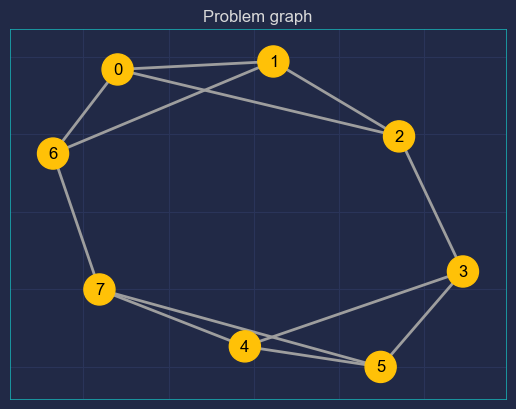
\includegraphics[width=0.55\textwidth]{Figures/Chapter_5/problem_graph.png}
    \caption{Considered $8$-node graph instance. The optimal cut ($10$) was found through
    brute-force (exhaustive search).}
    \label{fig:8_node_graph}
\end{figure}

%%%%%%%%%%%%%%%%%%%%%%%%%%%%%%%%%%%%%%%%%%%%%%%%%%%%%%%%%%%%%%%%%%%%%%%%
\section{Random iQAQE}
\label{section:Base_iQAQE}

% I think I'm going to be re-running many algorithms. This might take me some time, but I believe it is necessary.

First and foremost, we aim to understand how \acrshort{iqaqe} compares with both \acrshort{qaoa} and \acrshort{qemc}. In terms of \acrshort{iqaqe}'s implementation for this comparison, the number of qubits ($n$) and the list cardinalities ($c$) were selected without careful consideration. They were randomly chosen using \texttt{np.random.randint}, resulting in $n = 4$ and $c = 4$. Currently, the allocation of basis states to lists is also done randomly, without ensuring that all basis states are utilized. The goal of this initial simulation is to take a preliminary look at \acrshort{iqaqe}'s performance and understand how much the results vary between finite shot number simulations and analytical ones. (This also serves as a comparison test between the two previously mentioned PennyLane devices.) The plots below display the best-so-far average approximation ratio, derived from $10$ \acrshort{iqaqe} runs, each with different random initial parameters. The results for all three algorithms are generated using a configuration of $4$ ansatz layers and an Adam learning rate of $0.99$.

%%%%%%%%%%%%%%%%%%%%%%%%%%%%%%%%%%%%%%%%%%%%%%%%%%%%%%%%%%%%%%%%%%%%%%%%
\begin{figure}[ht!]
  \centering
  \begin{subfigure}[H]{0.495\textwidth}
      \centering
      \caption*{(a) Shots = None (Infinite)}
      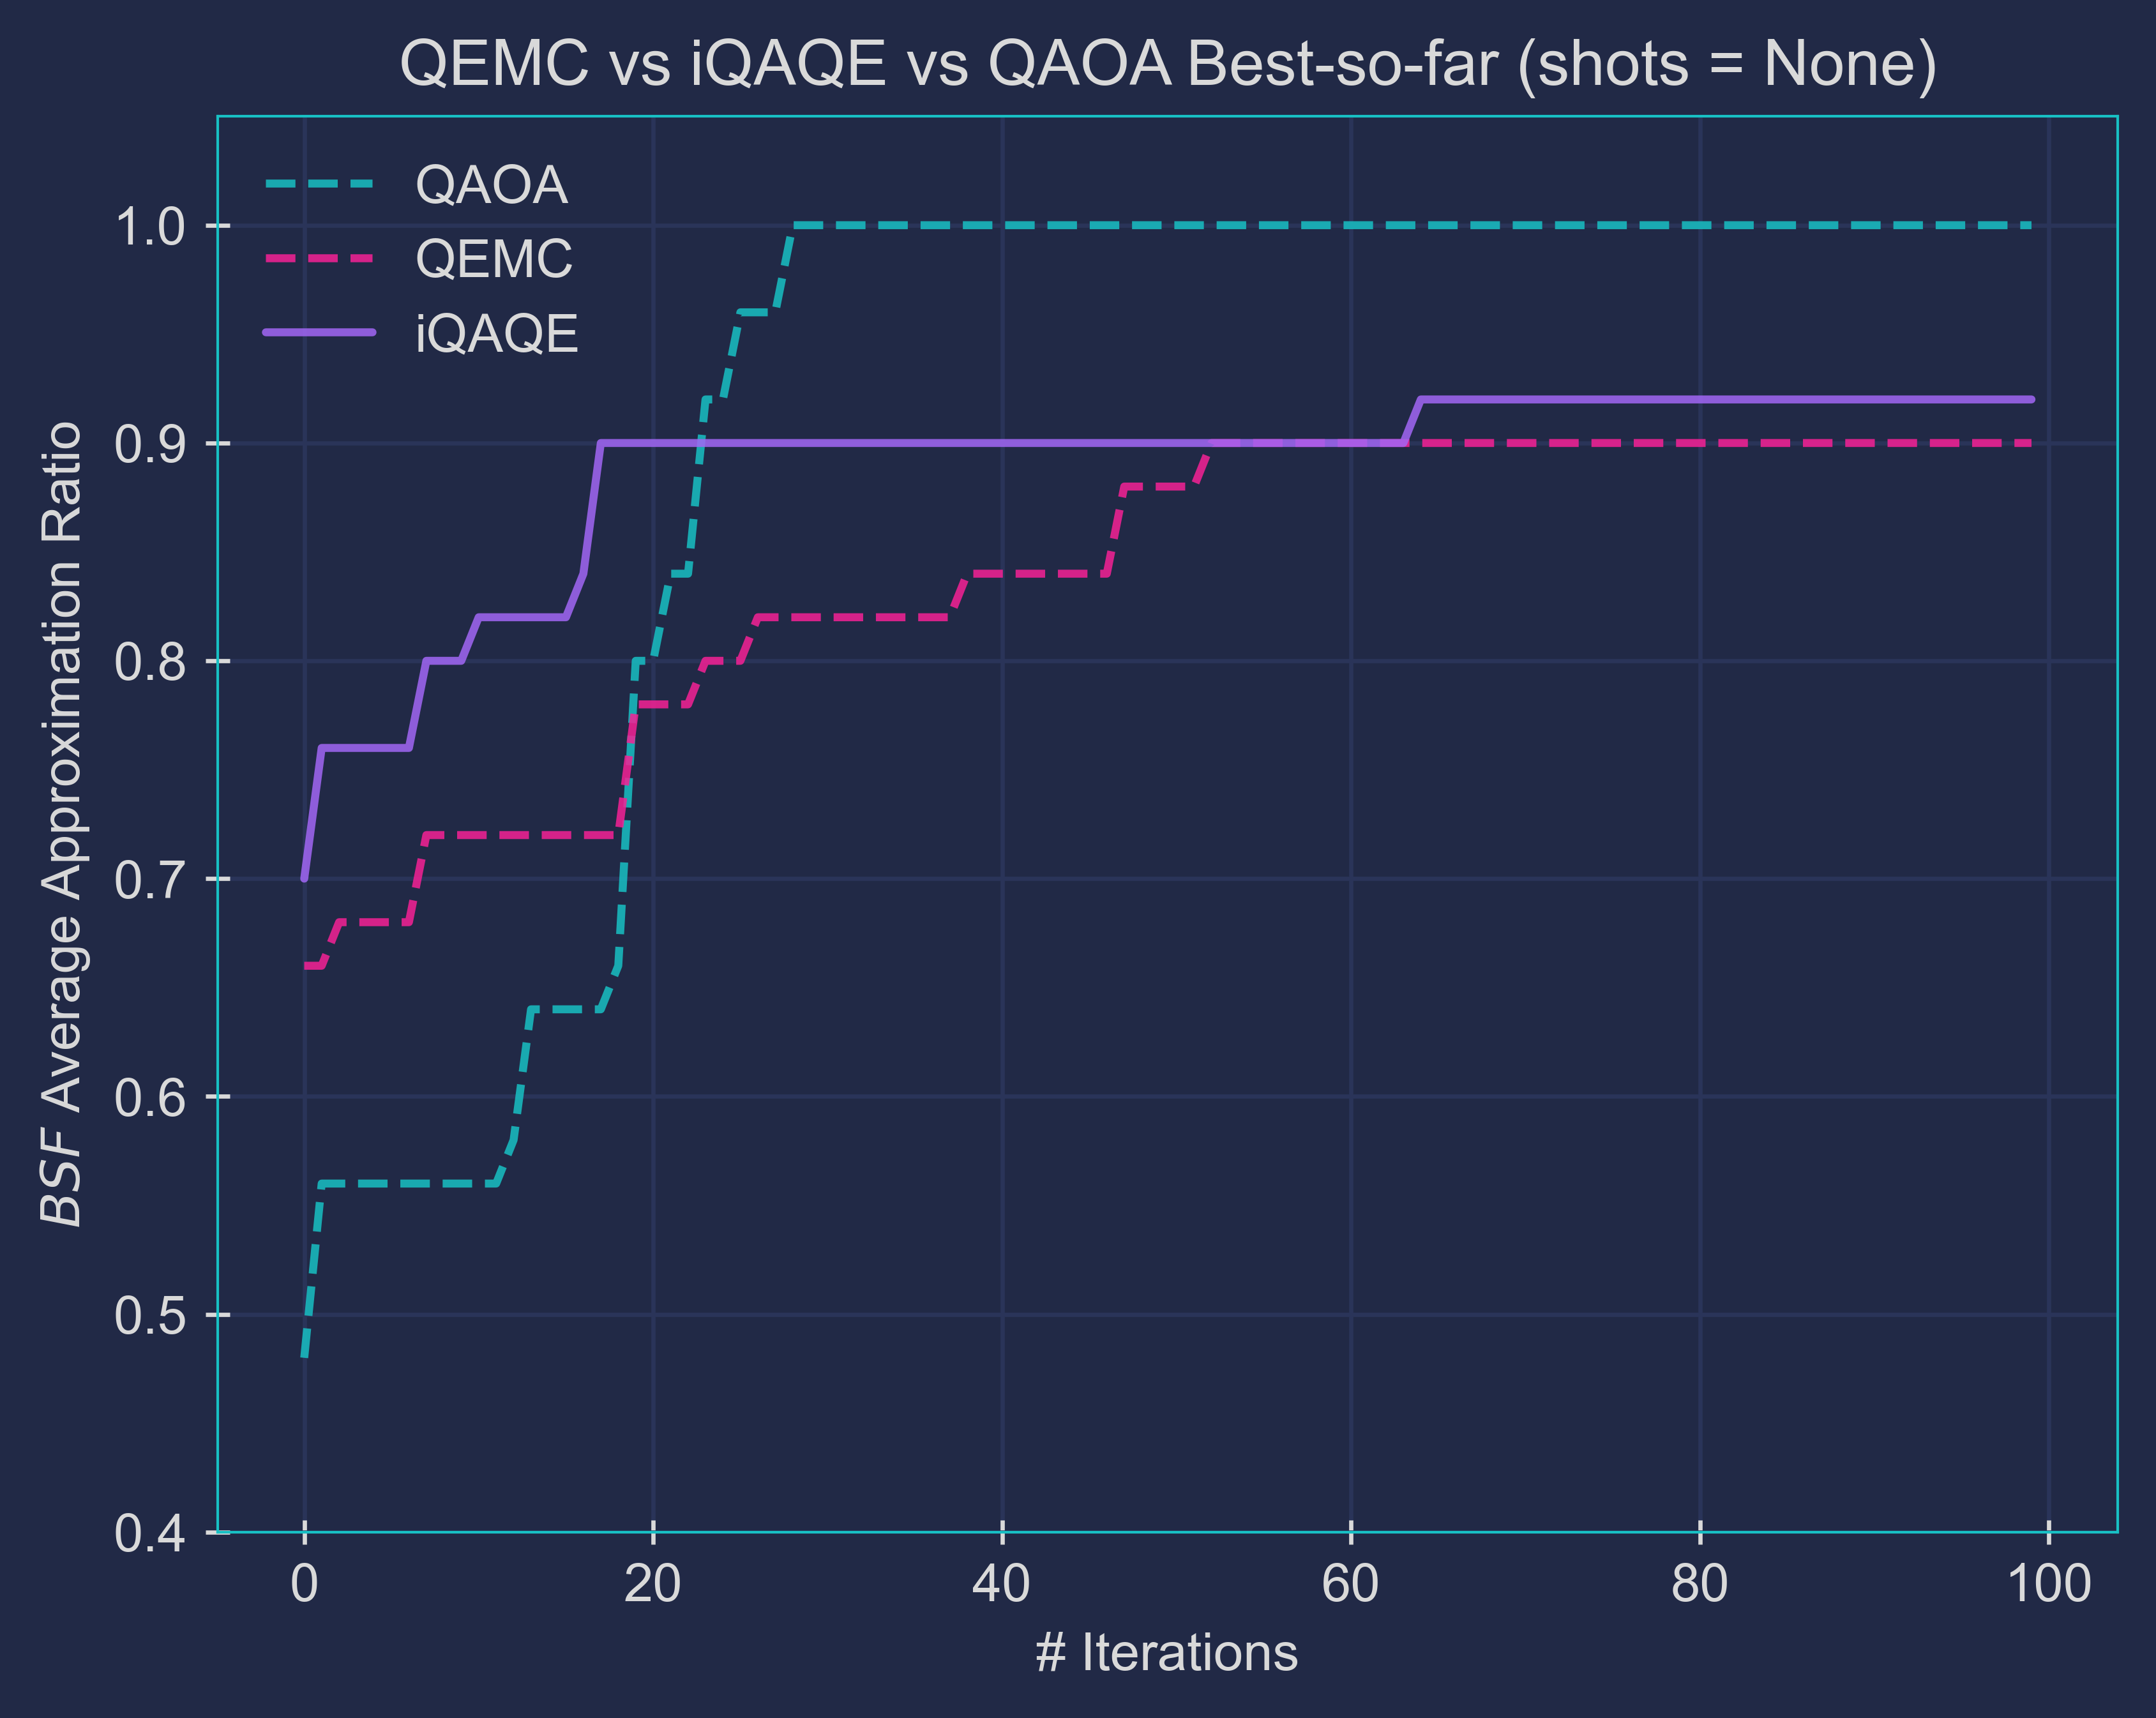
\includegraphics[width=1\textwidth]{Figures/Chapter_5/3_Comparison_None.png}
      \label{fig:3_Comparison_shots=None}
  \end{subfigure}
  % \hspace{-1.5em}
  \begin{subfigure}[H]{0.495\textwidth}
      \centering
      \caption*{(b) Shots = 1024}
      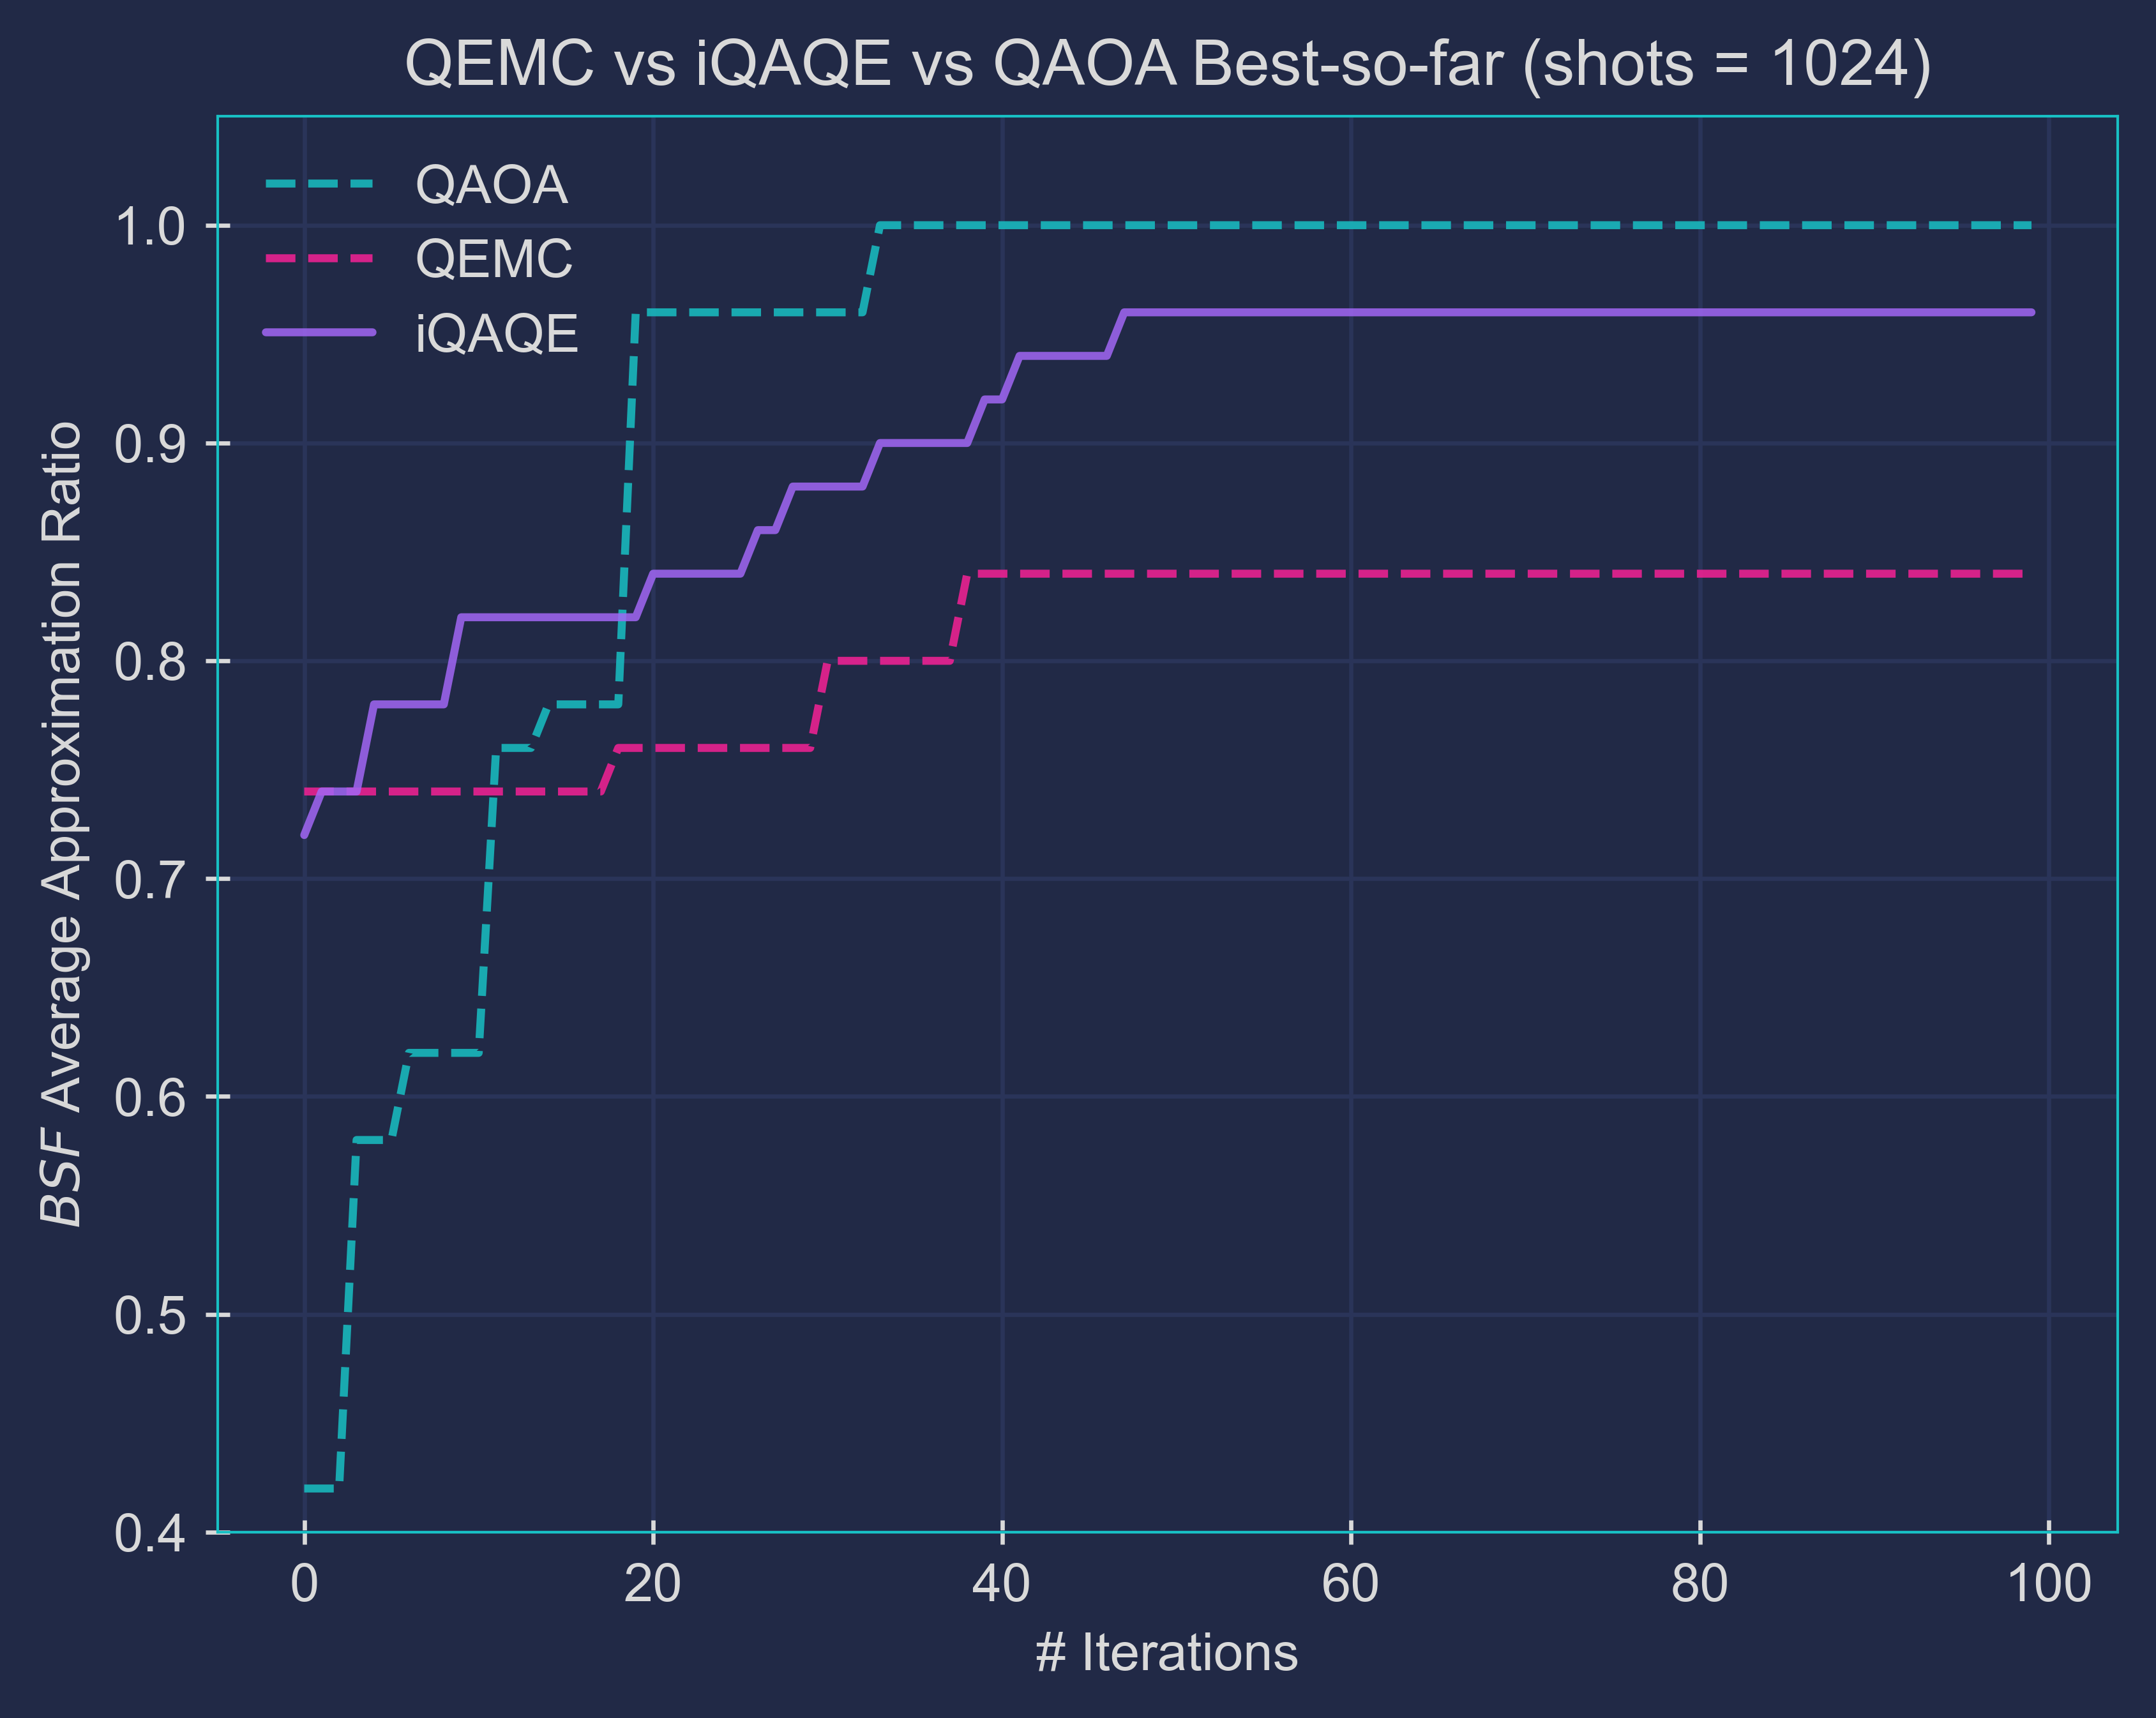
\includegraphics[width=1\textwidth]{Figures/Chapter_5/3_Comparison_1024.png}
      \label{fig:3_Comparison_shots=1024}
  \end{subfigure}

  % \vspace{-1.5em} % Adjust the space between the rows

  \begin{subfigure}[t]{0.495\textwidth}
      \centering
      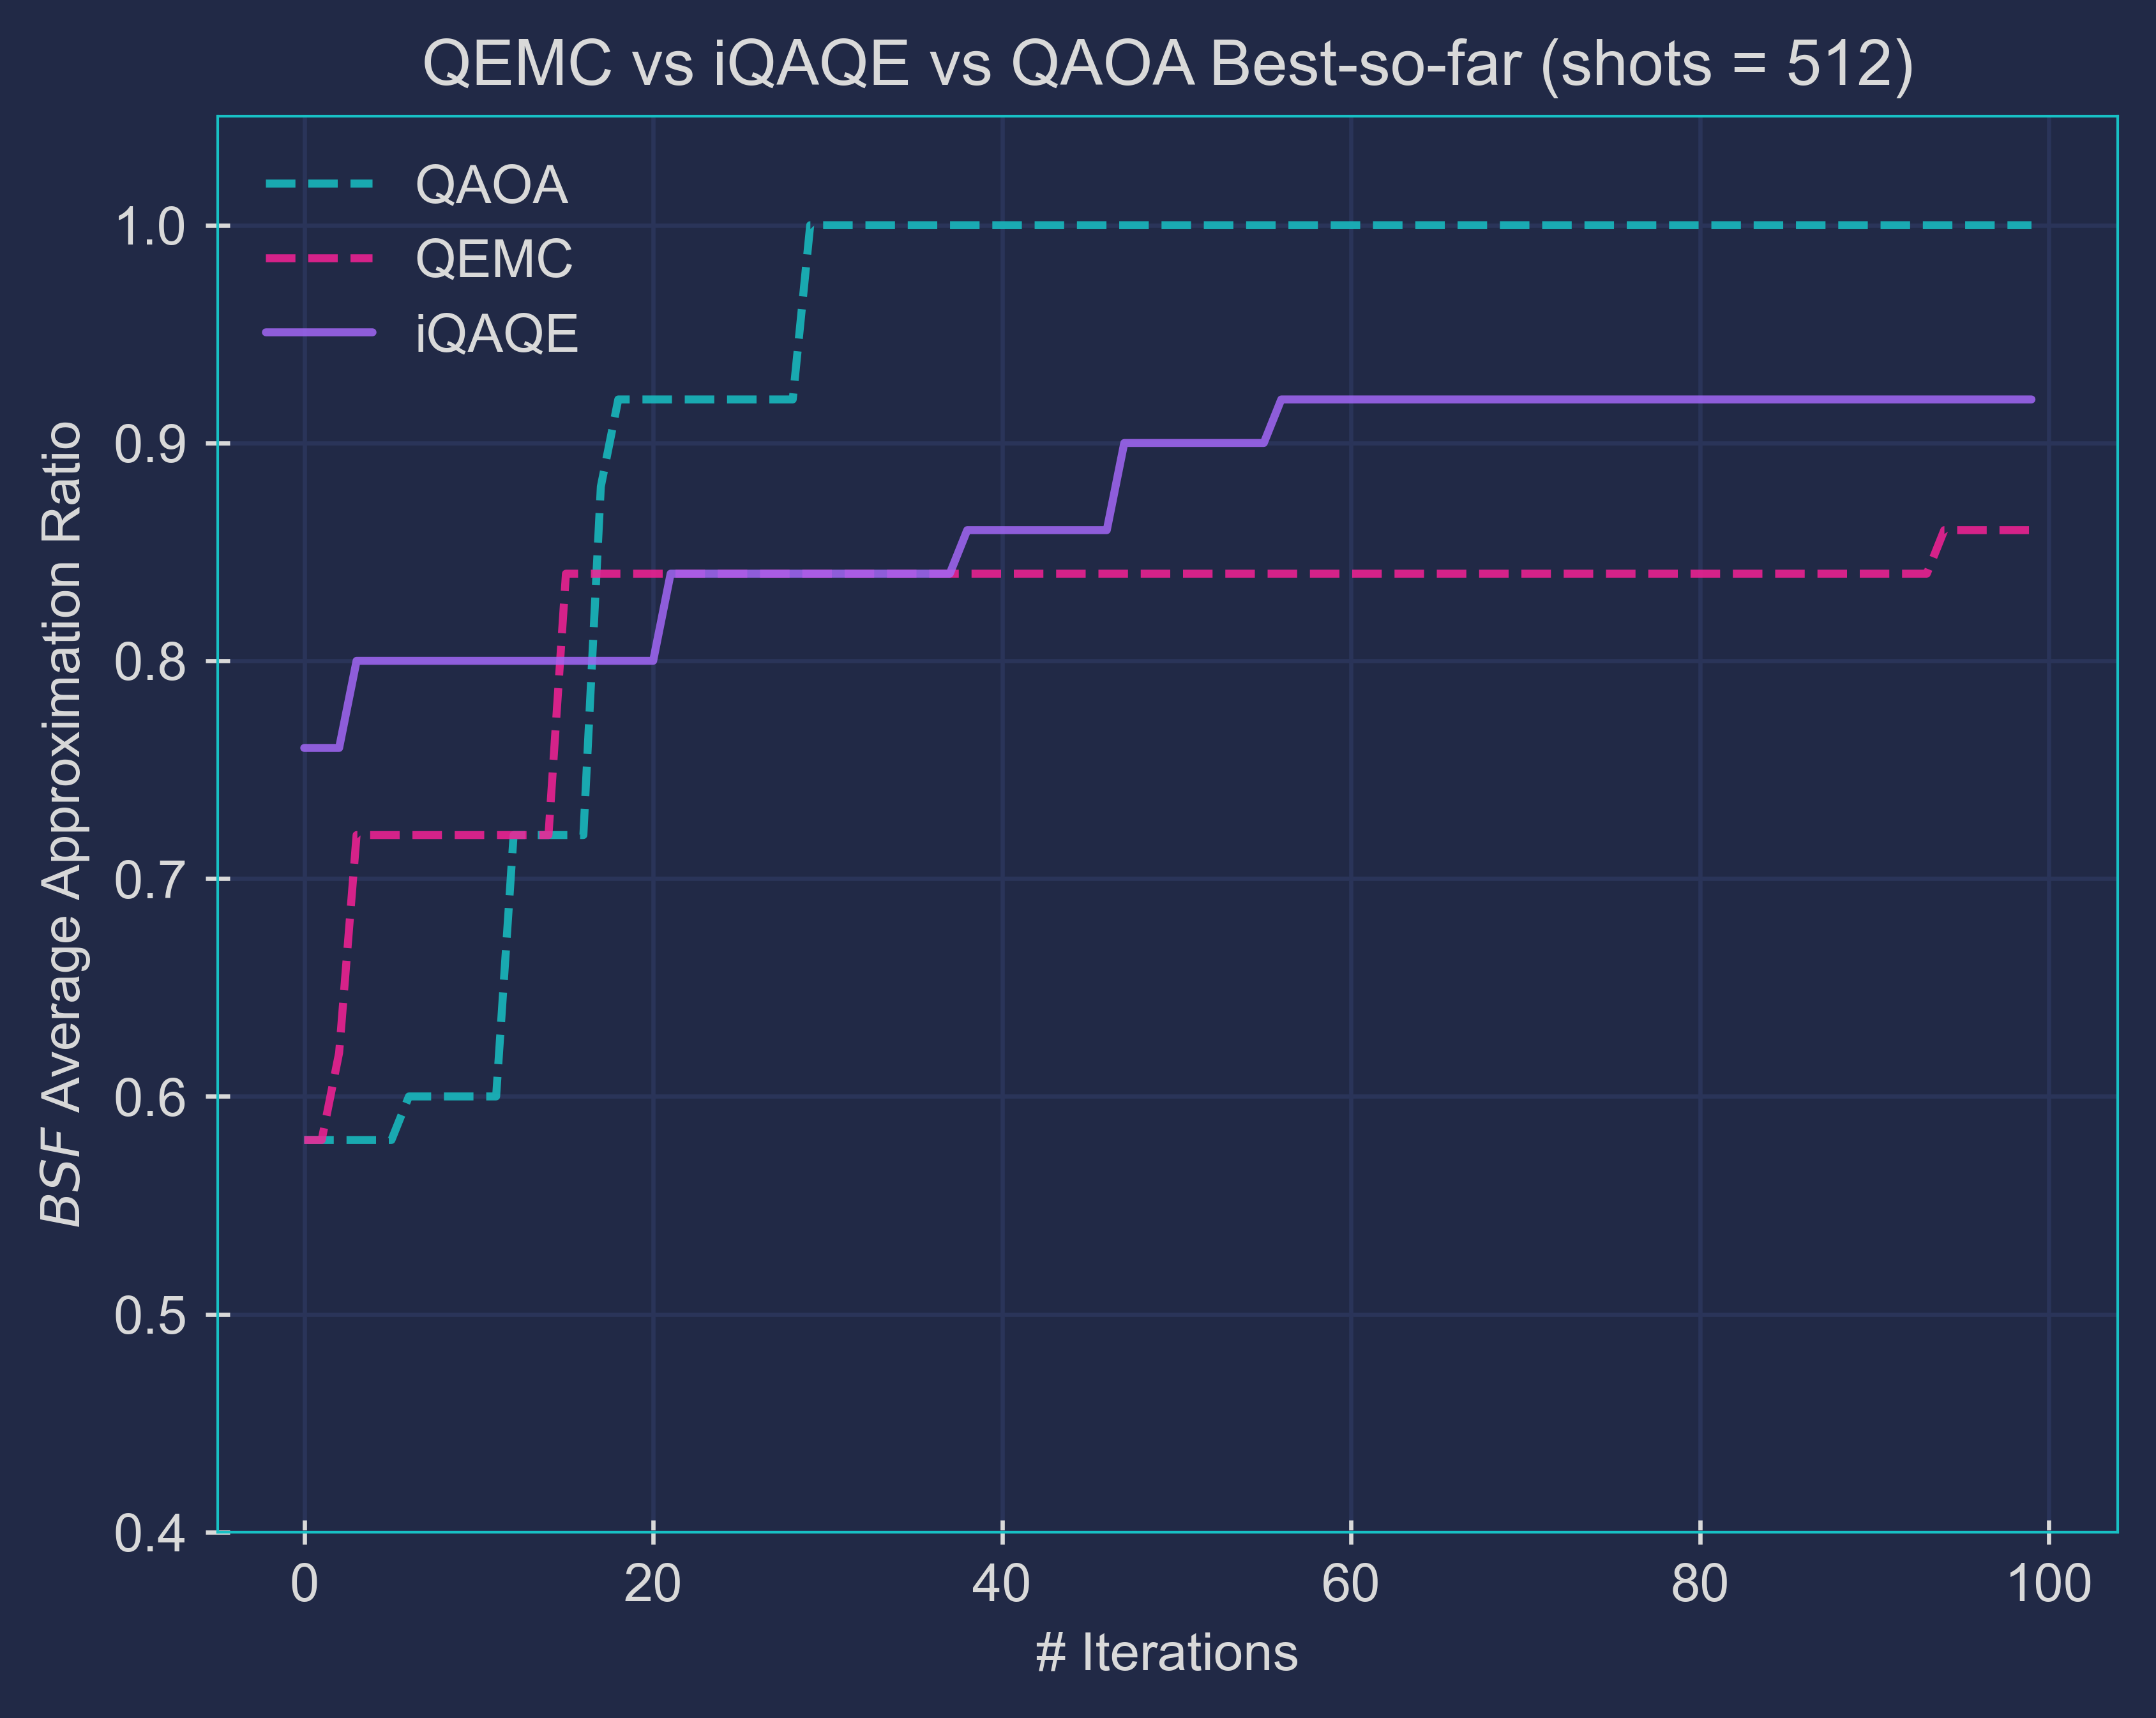
\includegraphics[width=1\textwidth]{Figures/Chapter_5/3_Comparison_512.png}
      \caption*{(c) Shots = 512}
      \label{fig:3_Comparison_shots=512}
  \end{subfigure}
  % \hspace{-1.5em}
  \begin{subfigure}[t]{0.495\textwidth}
      \centering
      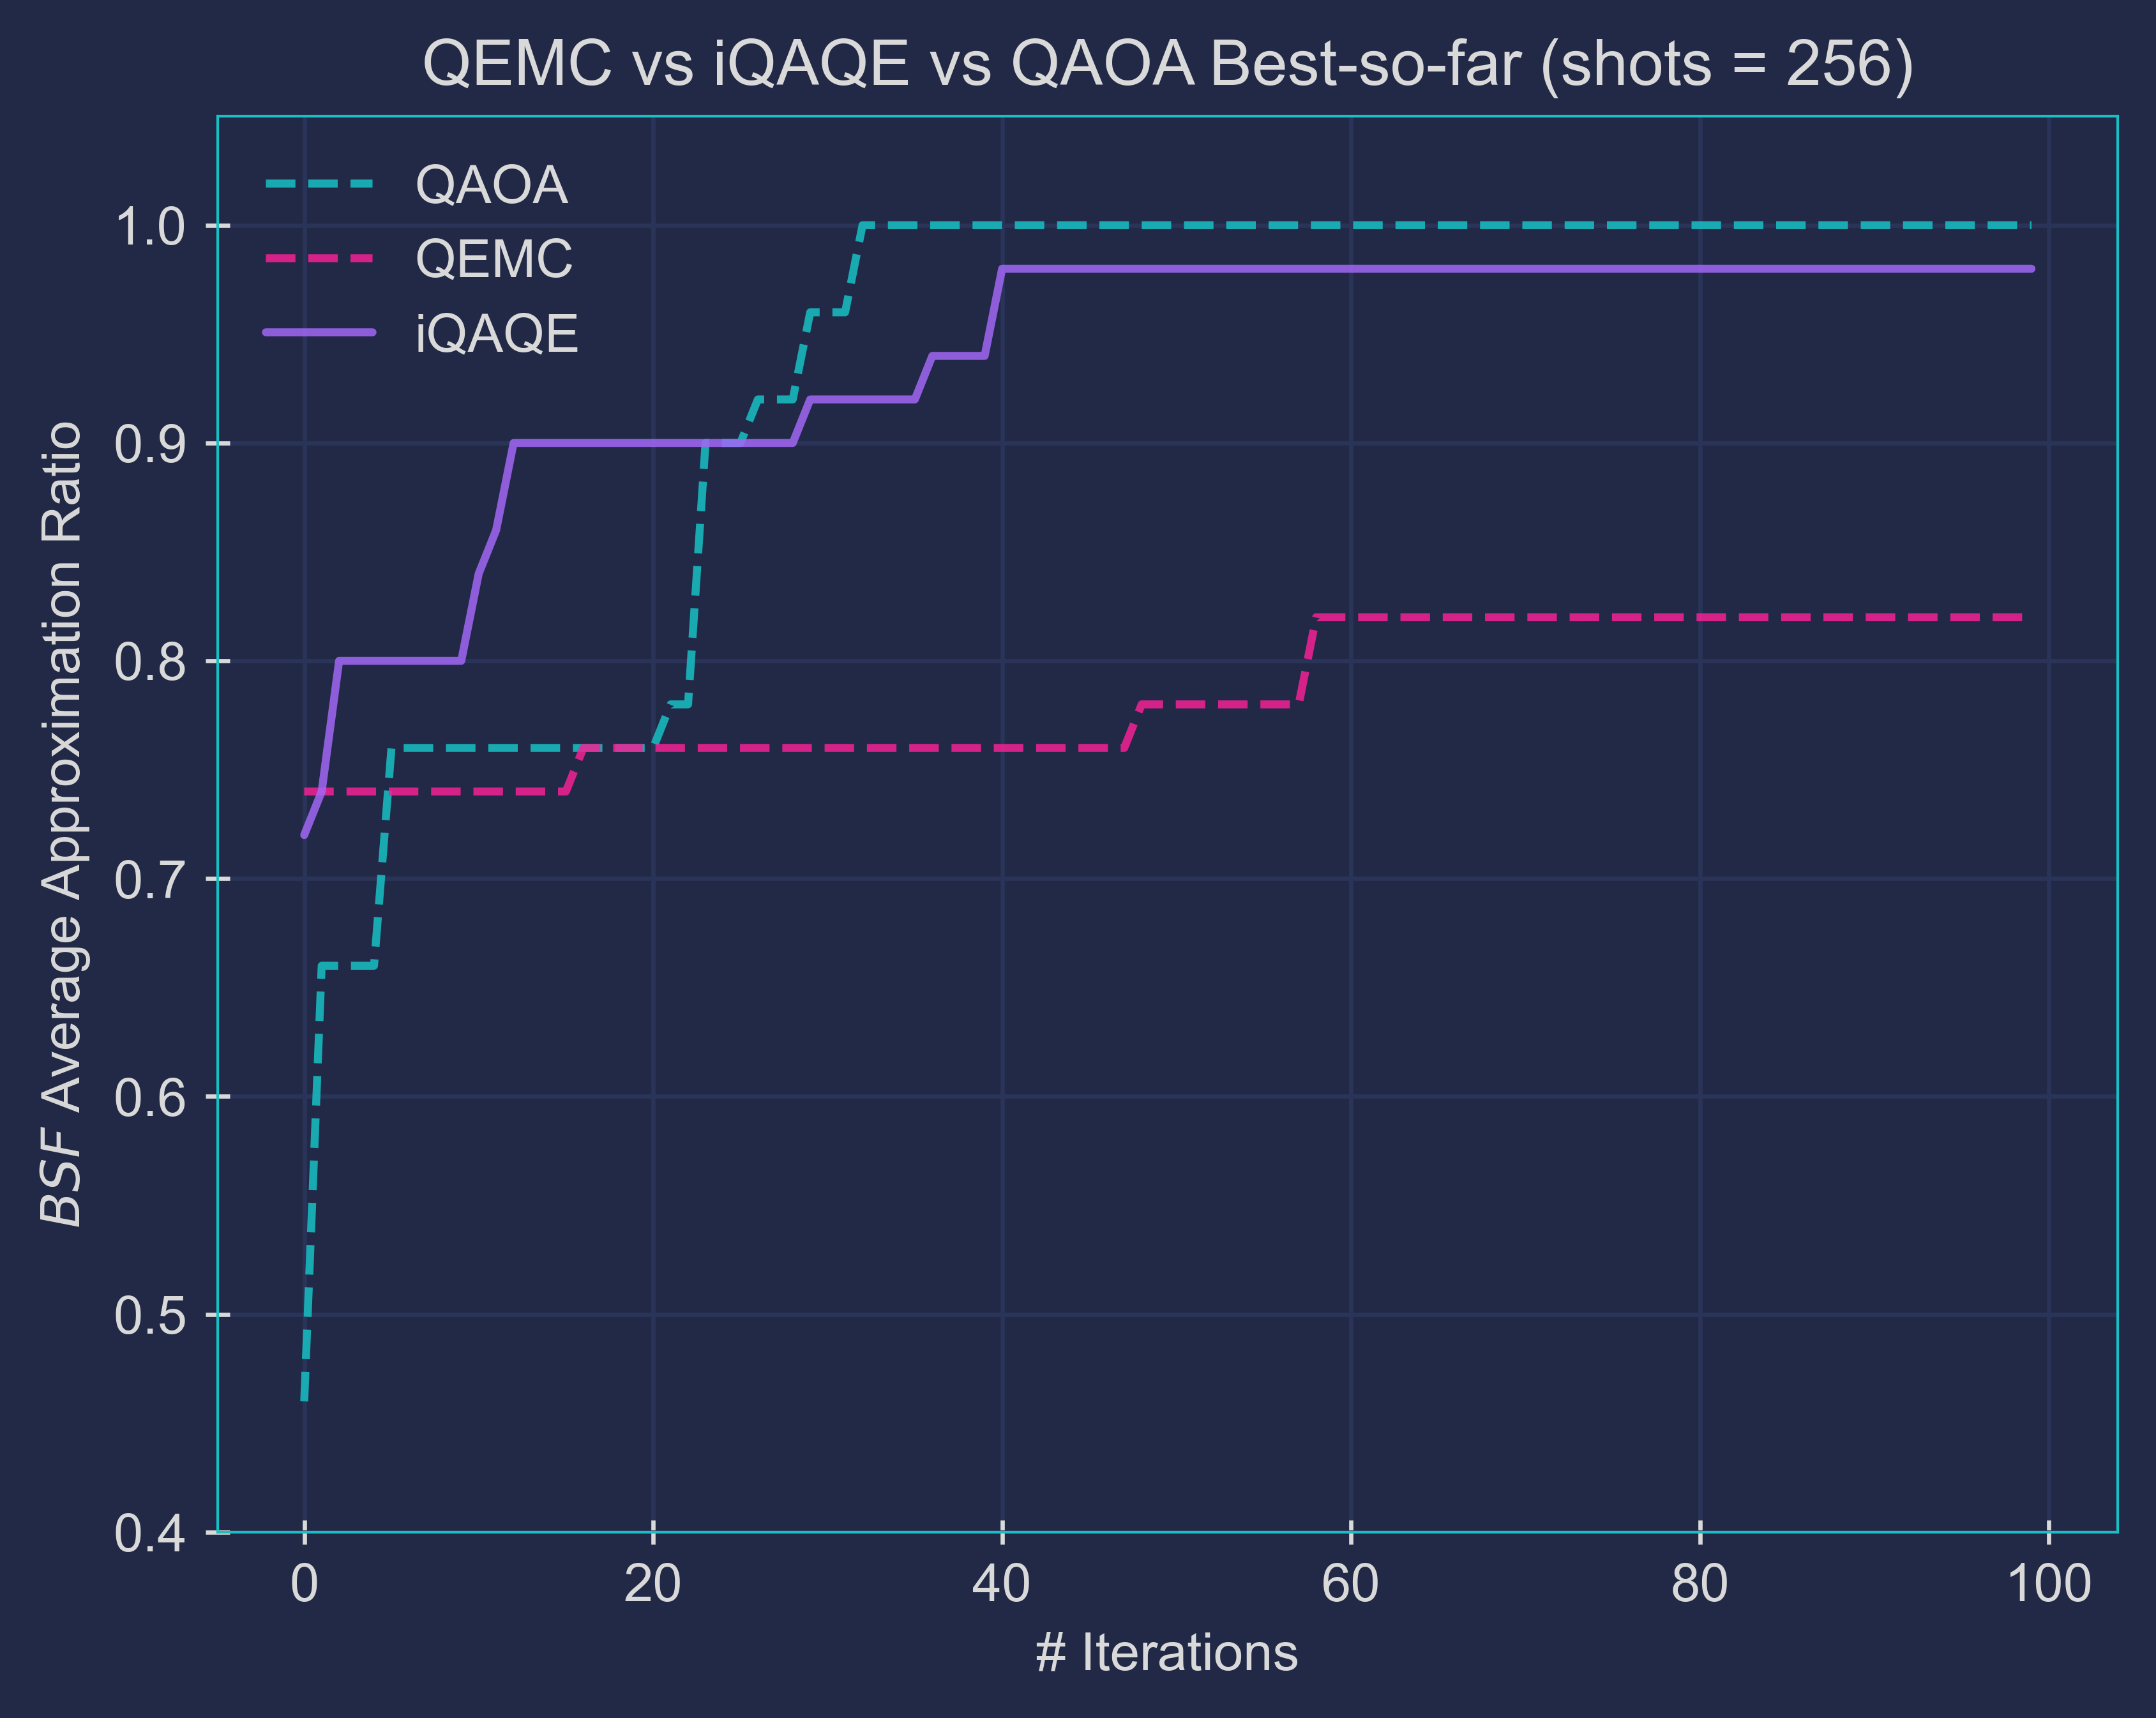
\includegraphics[width=1\textwidth]{Figures/Chapter_5/3_Comparison_256.png}
      \caption*{(d) Shots = 256}
      \label{fig:3_Comparison_shots=256}
  \end{subfigure}
  
  \caption{Comparison between the $3$ \acrshort{vqa}\textcolor{gray}{s}' performances (\acrshort{qaoa}, \acrshort{qemc} and \acrshort{iqaqe}), using an infinite and finite number of shots. The best-so-far average is plotted.}
  \label{fig:3_Comparison_shots}
\end{figure}
%%%%%%%%%%%%%%%%%%%%%%%%%%%%%%%%%%%%%%%%%%%%%%%%%%%%%%%%%%%%%%%%%%%%%%%%

These plots generally align with our theoretical expectations. As \acrshort{qemc} relies heavily on a large number of shots, transitioning to a finite shot number naturally impacts the results. Surprisingly, however, \acrshort{iqaqe} seems to exhibit slightly greater resilience to this effect, despite sharing \acrshort{qemc}'s cost function and ansatz. This resilience might be attributed to the presence of multiple basis states associated with each graph node, potentially reducing the need for exhaustive sampling. If some basis states are harder to sample, the probabilities of the remaining states might adapt to compensate, as governed by the \acrshort{qemc} objective function. Nonetheless, \acrshort{qaoa} consistently outperforms both approaches, highlighting its superiority. For the same number of layers, \acrshort{qaoa}'s problem-inspired ansatz and cost function consistently yield better results. To determine if \acrshort{iqaqe} can surpass \acrshort{qaoa}'s performance, extensive testing across various combinations of parameters such as $n$, $c$, number of layers, and Adam's learning rate is necessary. This will motivate some of the grid searches we conduct later in this study. However, given the vast number of potential combinations, testing all of them is impractical. Therefore, some of the more targeted mappings/encodings explored in this work aim to constrain one or more of these variables, thereby reducing the total number of combinations for testing. Following this approach, conducting grid searches over the parameter values becomes more manageable and practical to determine the optimal settings. The subsequent sections of this chapter will detail these mapping strategies.

%%%%%%%%%%%%%%%%%%%%%%%%%%%%%%%%%%%%%%%%%%%%%%%%%%%%%%%%%%%%%%%%%%%%%%%%
\section{Polynomial Compression-type Encodings}
\label{section:Polynomial_Encodings}

At this point, driven by our earlier discussion on the nature of random-based algorithms, we begin exploring more meaningful mappings. Here, we opt to fix one or more qubits to $1$ (or $0$) while allowing the remainder to vary. The number of qubits we fix ($k$) depends on the desired order of compression. This approach not only enables the utilization of fewer qubits (if $k > 1$) but also establishes the total number of qubits to be used, simplifying subsequent grid searches over parameters. By fixing $k$ qubits, we achieve polynomial compression of order-$k$ (in the number of qubits). The total number of nodes that can be encoded in this manner is determined by $\binom{n}{k} = \frac{n!}{k!(n - k)!}$, where $n$ denotes the number of qubits. Essentially, this represents the number of ways we can select $k$ qubits from the available $n$ and set them to $1$ (or $0$), each combination encoding one graph node. Consequently, we need to ensure that $\binom{n}{k} \geq N$, where $N$ represents the number of graph nodes. This criterion guides our selection of $n$ and $k$. In practice, to determine $n$ for any $k$, we select the smallest $n$ that satisfies $\binom{n}{k} \geq N$. This yields $N = \mathcal{O}(n^k)$. Subsequently, we decide on the number of basis states to associate with each graph node, chosen from a total of $2^{n-k}$. While we could potentially utilize all $2^{n-k}$ basis states for each node (with $n-k$ free qubits), we allow for the flexibility to choose only $c \leq 2^{n-k}$. The value of $c$ requires optimization. With the mapping established, the algorithm proceeds as before, employing \acrshort{qemc}'s cost function and ansatz. Notably, we cannot use \acrshort{qaoa}'s ansatz since $n \neq N$. Due to polynomial compression, $n < N$ always, unless $k = 1$ (in which case there is no compression).






%%%%%%%%%%%%%%%%%%%%%%%%%%%%%%%%%%%%%%%%%%%%%%%%%%%%%%%%%%%%%%%%%%%%%%%%
\subsection{Basic Polynomial Compression-type iQAQE}
\label{subsection:Basic_Poly-Comp_iQAQE}


This is the simplest type of polynomial compression-based \acrshort{iqaqe} scheme. It involves fixing $k$ qubits to $1$ instead of $0$ (e.g., $\{\ket{11\text{xxx}}\}$, for $k = 2$). The number of fixed qubits ($k$) is determined by the desired order of compression, as previously described. The results for $k = 2$ and $k = 3$ are shown below (Figures \ref{fig:Comparison_k2+k3_1} and \ref{fig:Comparison_k2+k3_2}). In the figures, the list cardinality is set to $4$ for both the $k = 2$ curves (\texttt{iQAQE\_k2}) and the $k = 3$ curves (\texttt{iQAQE\_k3}). Additionally, the number of layers is set to $4$ for $k = 2$ and $5$ for $k = 3$, with an Adam learning rate of $0.98$. The final curves are derived from $10$ runs of the algorithms, each with different random initial parameters. The results are compared with those of \acrshort{qaoa} and \acrshort{qemc}.

\begin{figure}[H]
  \centering
  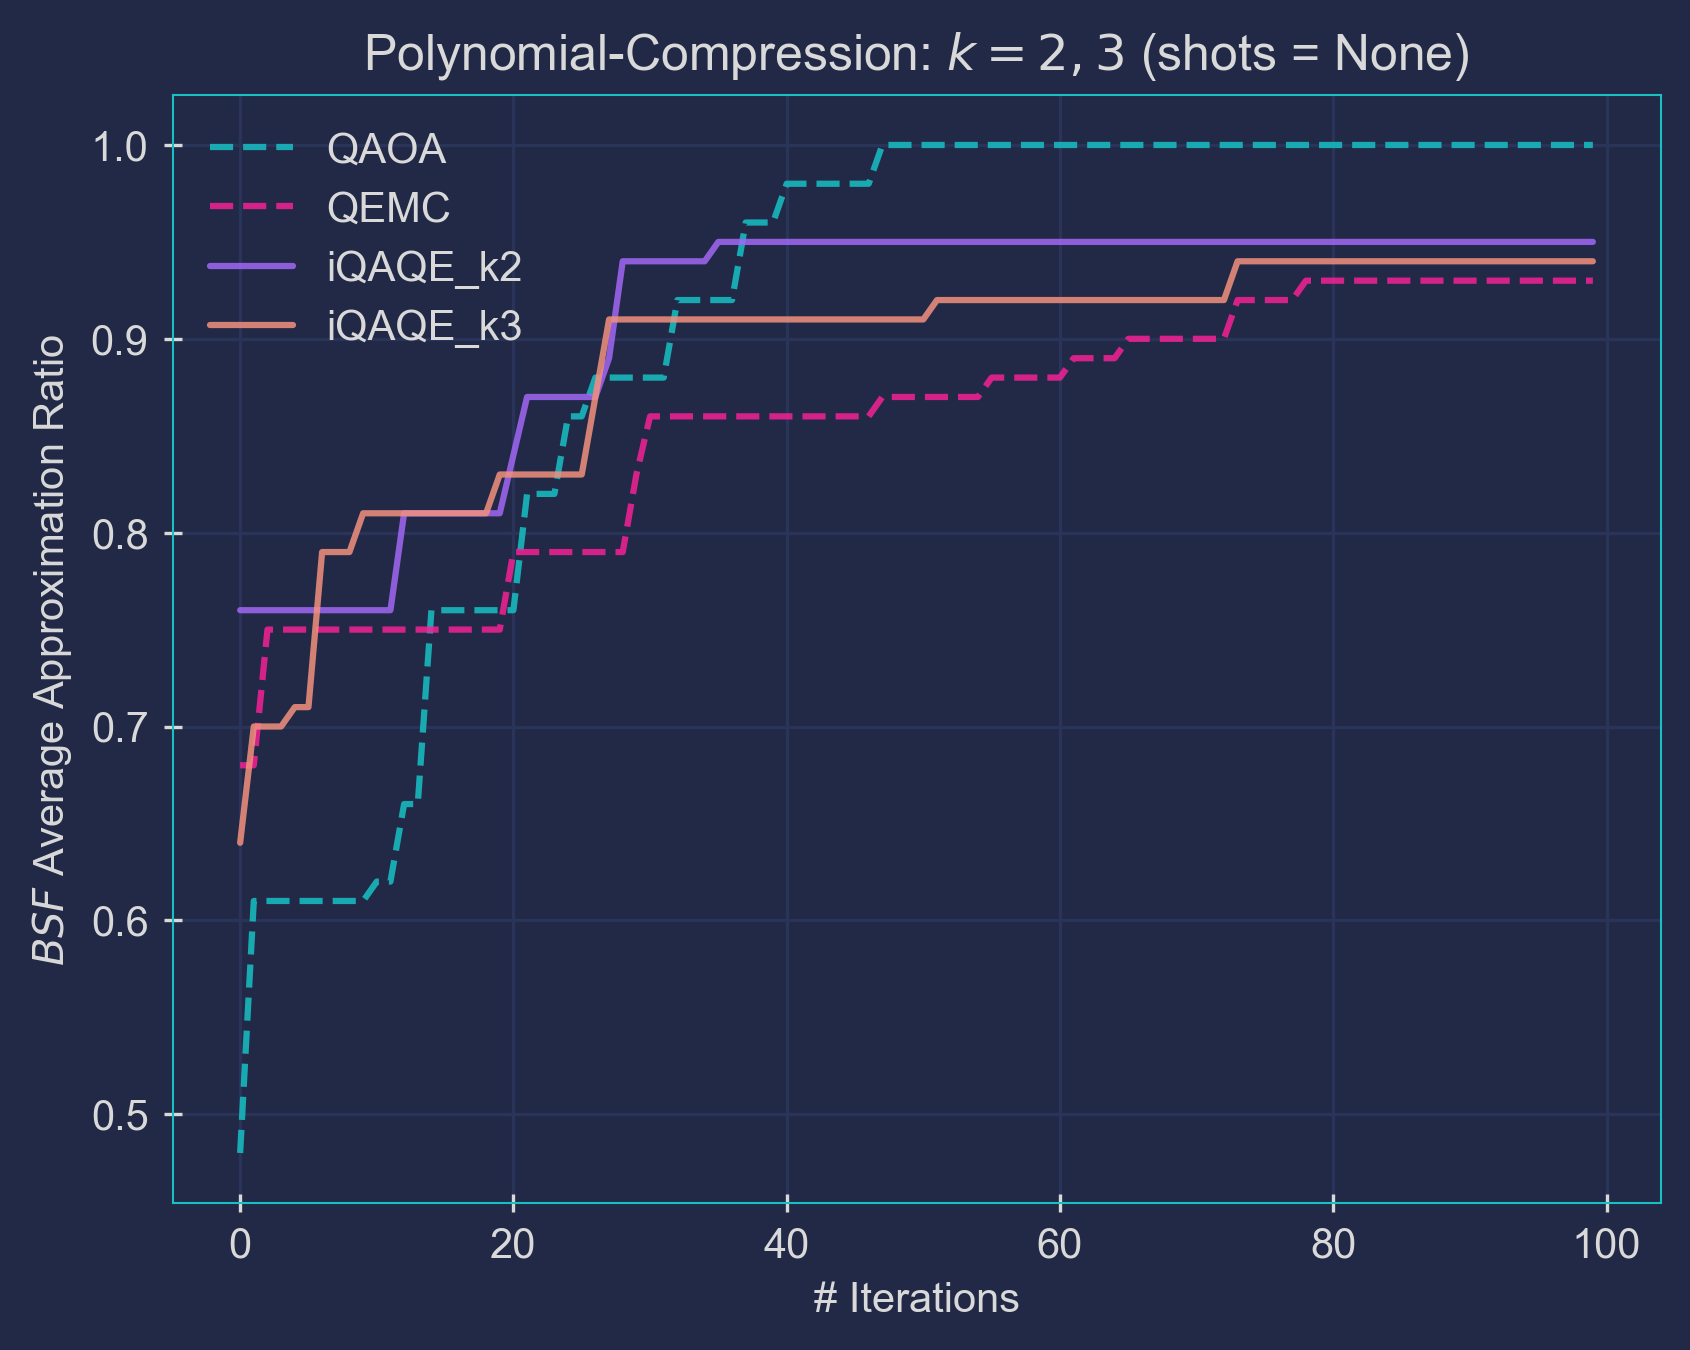
\includegraphics[width=0.675\textwidth]{Figures/Chapter_5/Polynomial_Compression_Base_k2_k3_2.png}
  \caption{\acrshort{bsf} Average Approximation Ratio \textit{vs.} iteration number for the tested \acrshort{vqa}\textcolor{gray}{s}: \acrshort{qaoa}, \acrshort{qemc}, and \acrshort{iqaqe}, using the aforementioned polynomial compression scheme. The number of layers considered were $4$ for $k = 2$ and $5$ for $k = 3$.}
  \label{fig:Comparison_k2+k3_1}
\end{figure}

\begin{figure}[H]
  \centering
  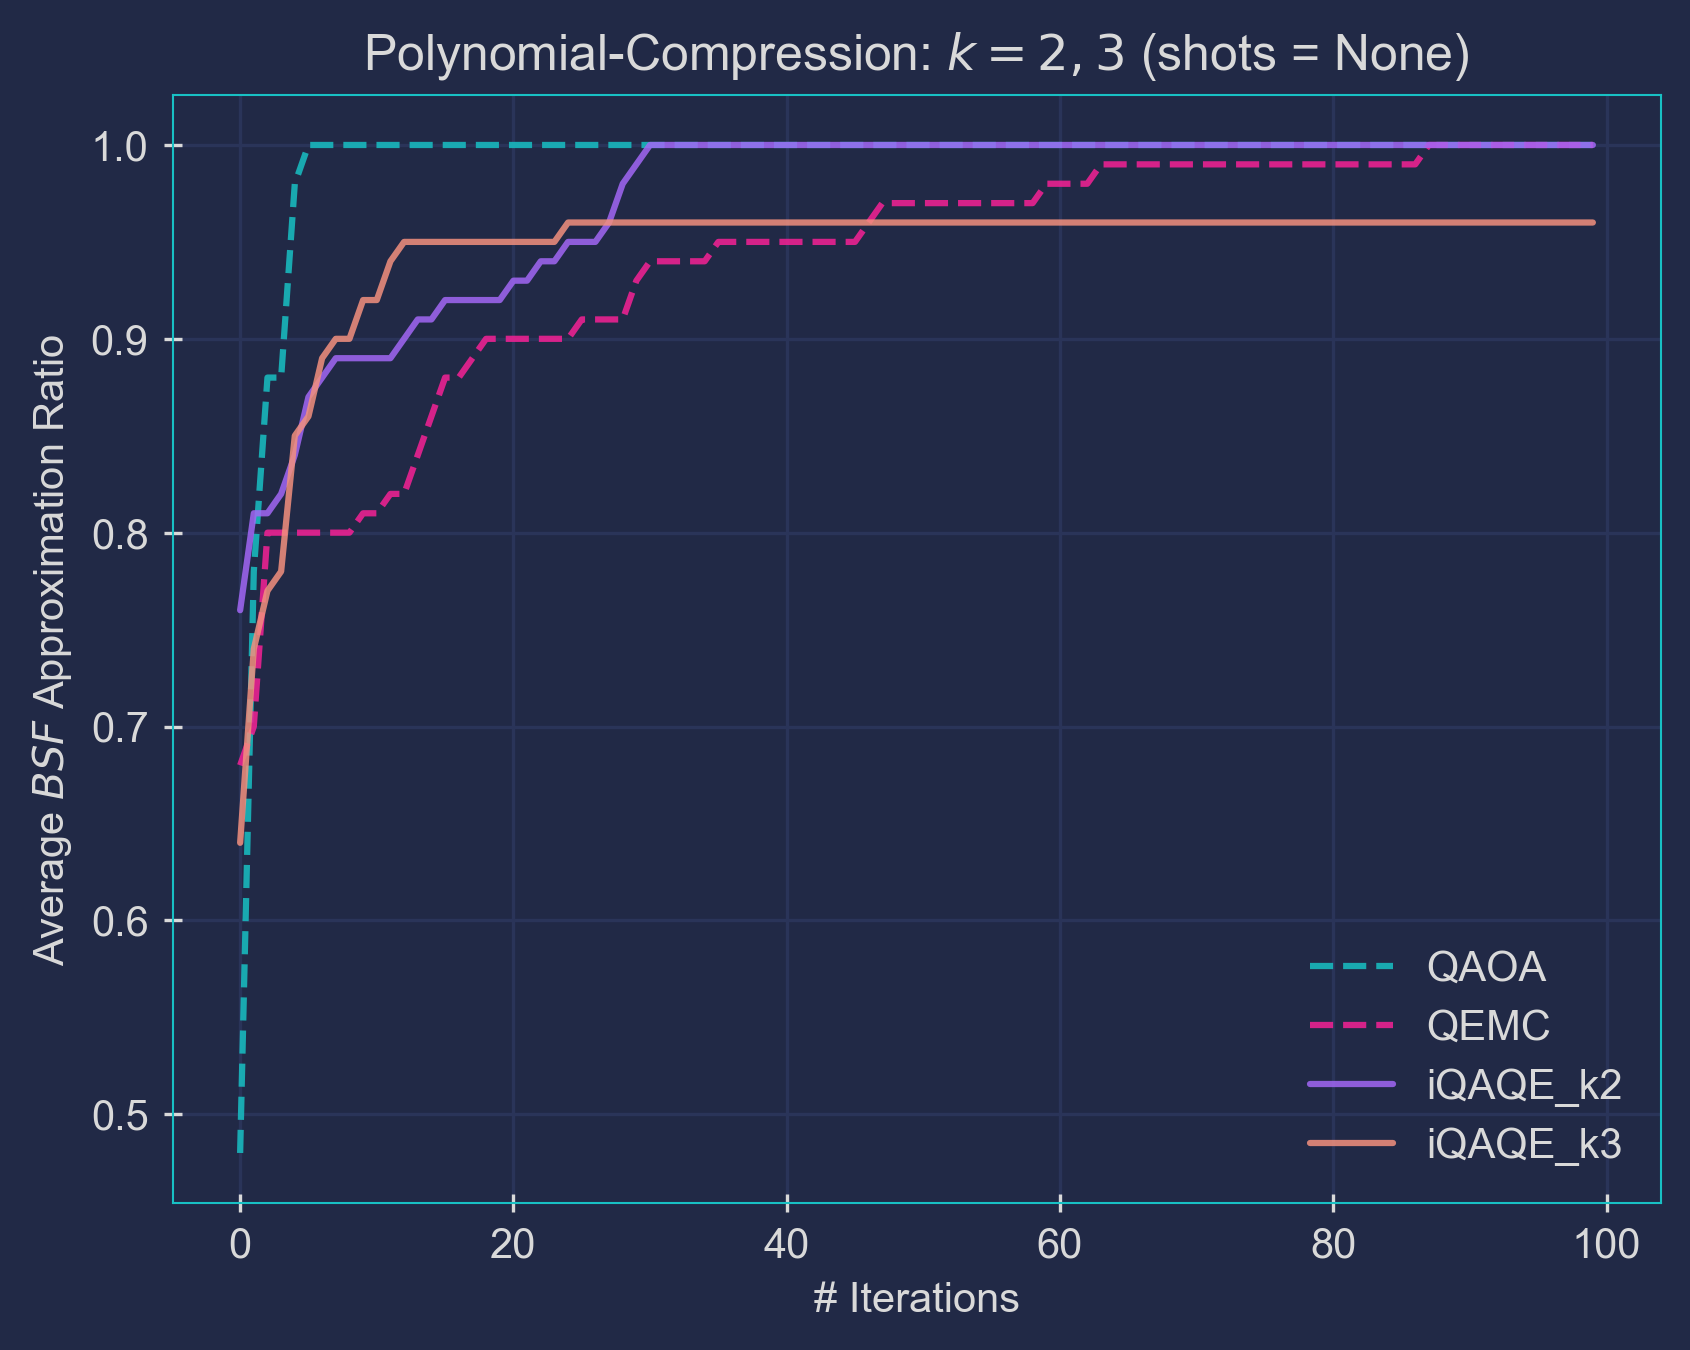
\includegraphics[width=0.675\textwidth]{Figures/Chapter_5/Polynomial_Compression_Base_k2_k3_1.png}
  \caption{Average \acrshort{bsf} Approximation Ratio \textit{vs.} iteration number for the tested \acrshort{vqa}\textcolor{gray}{s}: \acrshort{qaoa}, \acrshort{qemc}, and \acrshort{iqaqe}, using the aforementioned polynomial compression scheme. The number of layers considered were $4$ for $k = 2$ and $5$ for $k = 3$.}
  \label{fig:Comparison_k2+k3_2}
\end{figure}



Notice the difference between the two figures. In the first figure, we average the curves first and then apply the \acrshort{bsf} transformation. In the second figure, we reverse the process: first applying the \acrshort{bsf} transformation to each curve and then averaging the transformed curves. The results are quite different, as illustrated. This suggests that both \acrshort{qemc} and \acrshort{iqaqe} are typically more sensitive to fluctuations in their performance curves, hinting at a more complex optimization landscape. This is an important consideration when interpreting the forthcoming results. Often, we will choose to discard the \acrshort{bsf} average in favor of the average \acrshort{bsf} (cf. section \ref{section:BSF_correction}). Nonetheless, both approaches are valuable for evaluating the algorithms' properties. Additionally, in some instances, we will simply use the average. Each case will be clearly specified.

% This indicates that both \acrshort{qemc} and \acrshort{iqaqe} are generally more susceptible to outliers due to particularly unlucky initial parameterizations. 

Anyways, the primary aim of this study was to assess whether different types of mappings, like the one explored here, offer advantages compared to the random case. The results in Figures \ref{fig:Comparison_k2+k3_1} and \ref{fig:Comparison_k2+k3_2} indicate that this may be the case. At the very least, they suggest that there is potential in exploring these ideas further. For example, \texttt{iQAQE\_k2} achieves a perfect approximation ratio (Figure \ref{fig:Comparison_k2+k3_2}), although it requires more iterations [to get there] than \acrshort{qaoa}. Nevertheless, our method surpasses \acrshort{qemc} for $k = 2$. The results for $k = 3$ are less encouraging. However, both mappings use fewer qubits ($n = 5$) than \acrshort{qaoa} ($n = 8$), which is beneficial for implementation on practical (\acrshort{nisq}) quantum computers. The next step is to conduct grid searches over the parameters for this specific graph instance to determine if we can consistently achieve better performance than \acrshort{qaoa}. This might provide further insights into the underlying principles of the algorithm's performance.

% k=2:
\begin{figure*}[ht!]
  \centering
  \begin{subfigure}[b]{0.325\textwidth}
      \centering
      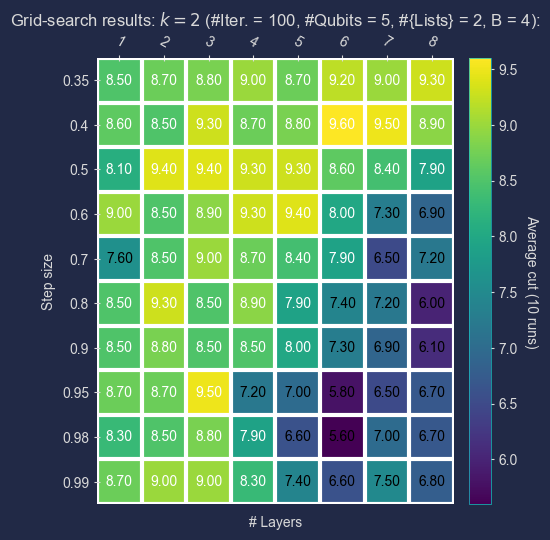
\includegraphics[width=1\textwidth]{Figures/Chapter_5/k=2(Grid_Search)/iQAQE_k2_Grid_Search_step_size_n_layers_c=2.png}
      \caption{\texttt{k = 2; c = 2}}
      \label{fig:k=2;c=2}
  \end{subfigure}
  \hfill
  \begin{subfigure}[b]{0.325\textwidth}
      \centering
      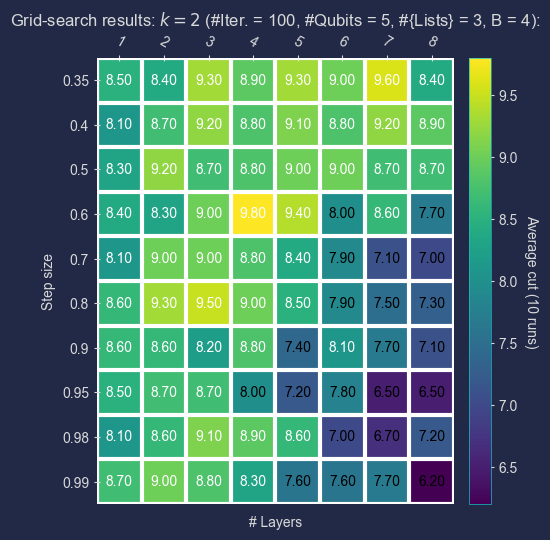
\includegraphics[width=1\textwidth]{Figures/Chapter_5/k=2(Grid_Search)/iQAQE_k2_Grid_Search_step_size_n_layers_c=3.png}
      \caption{\texttt{k = 2; c = 3}}
      \label{fig:k=2;c=3}
  \end{subfigure}
  \hfill
      \begin{subfigure}[b]{0.325\textwidth}
      \centering
      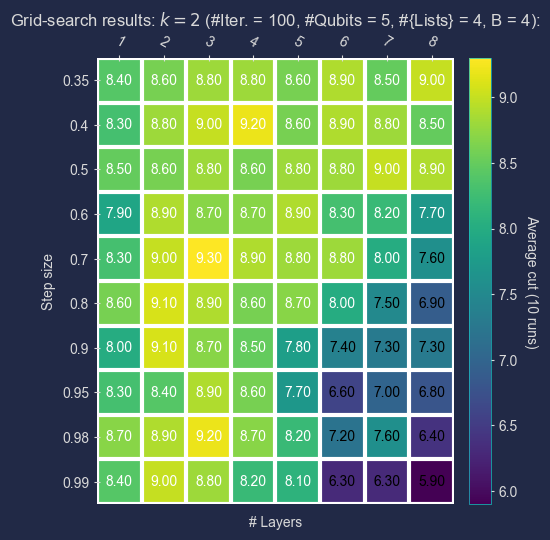
\includegraphics[width=1\textwidth]{Figures/Chapter_5/k=2(Grid_Search)/iQAQE_k2_Grid_Search_step_size_n_layers_c=4.png}
      \caption{\texttt{k = 2; c = 4}}
      \label{fig:k=2;c=4}
  \end{subfigure}
  \bigskip
  \begin{subfigure}[b]{0.325\textwidth}
      \addtocounter{subfigure}{3} % Added <<
      \centering
      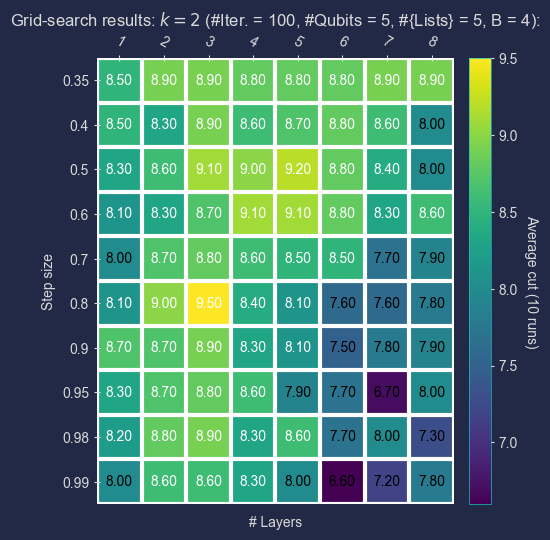
\includegraphics[width=1\textwidth]{Figures/Chapter_5/k=2(Grid_Search)/iQAQE_k2_Grid_Search_step_size_n_layers_c=5.png}
      \caption{\texttt{k = 2; c = 5}}
      \label{fig:k=2;c=5}
  \end{subfigure}
  \hfill
  \begin{subfigure}[b]{0.325\textwidth}
      \centering
      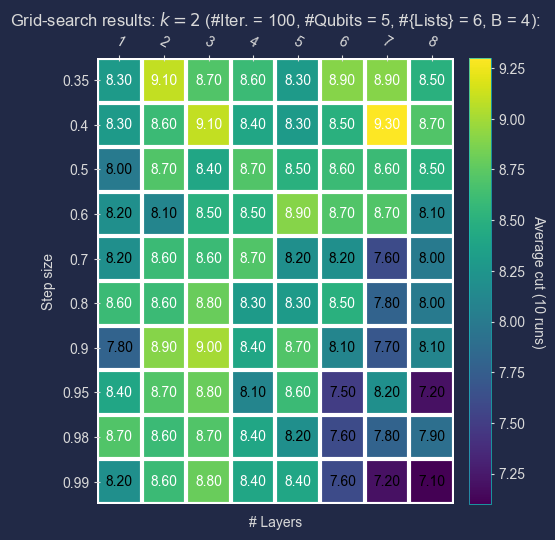
\includegraphics[width=1\textwidth]{Figures/Chapter_5/k=2(Grid_Search)/iQAQE_k2_Grid_Search_step_size_n_layers_c=6.png}
      \caption{\texttt{k = 2; c = 6}}
      \label{fig:k=2;c=6}
  \end{subfigure}
  \hfill
  \begin{subfigure}[b]{0.325\textwidth}
      \centering
      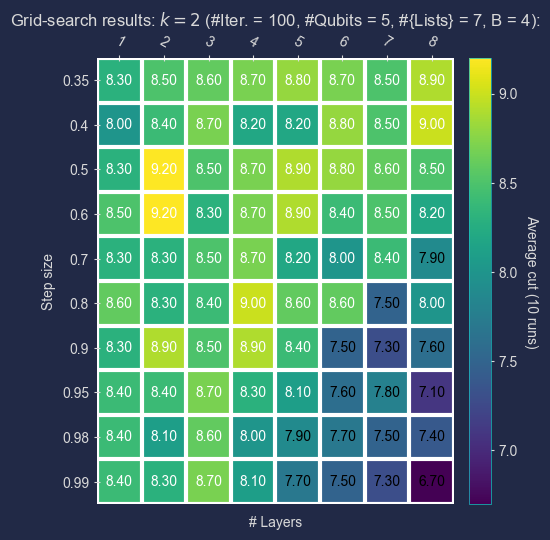
\includegraphics[width=1\textwidth]{Figures/Chapter_5/k=2(Grid_Search)/iQAQE_k2_Grid_Search_step_size_n_layers_c=7.png}
      \caption{\texttt{k = 2; c = 7}}
      \label{fig:k=2;c=7}
  \end{subfigure}
  \caption{Basic Polynomial Compression-type \acrshort{iqaqe} – grid search, using $k=2$. All the simulations were done using an infinite number of shots (\texttt{shots = None}), and each value consists of the average of $10$ \acrshort{iqaqe} instances, using different random initial parameters.}
  \label{fig:k=2}
\end{figure*}

% k=3:
\begin{figure*}[ht!]
  \centering
  \begin{subfigure}[b]{0.475\textwidth}
      \centering
      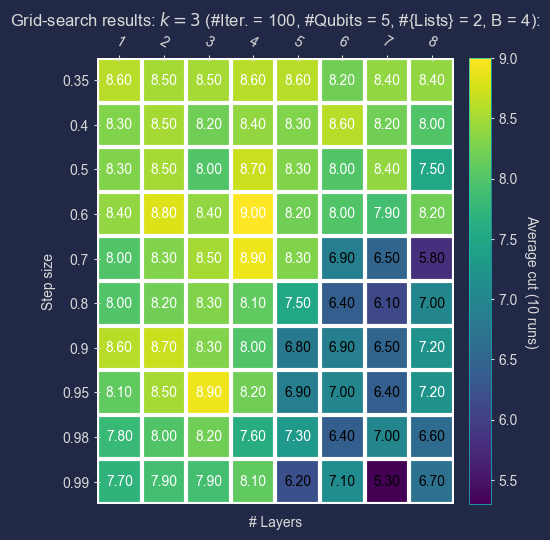
\includegraphics[width=1\textwidth]{Figures/Chapter_5/k=3(Grid_search)/iQAQE_k3_Grid_Search_step_size_n_layers_c=2.png}
      \caption{\texttt{k = 3; c = 2}}
      \label{fig:k=3;c=2}
  \end{subfigure}
  \hfill
  \begin{subfigure}[b]{0.475\textwidth}
      \centering
      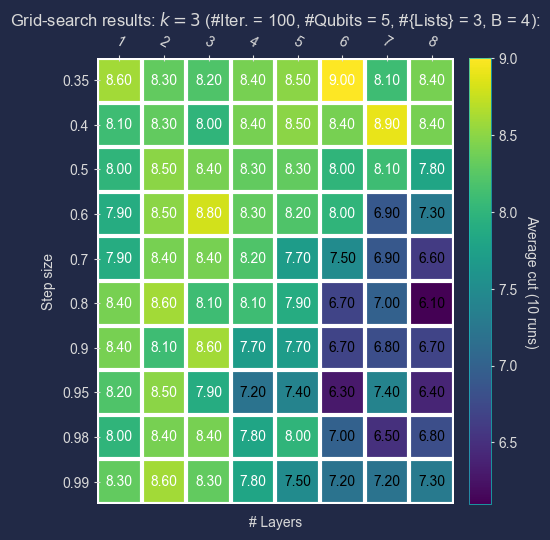
\includegraphics[width=1\textwidth]{Figures/Chapter_5/k=3(Grid_search)/iQAQE_k3_Grid_Search_step_size_n_layers_c=3.png}
      \caption{\texttt{k = 3; c = 3}}
      \label{fig:k=3;c=3}
  \end{subfigure}
  \caption{Basic Polynomial Compression-type \acrshort{iqaqe} – grid search, using $k=3$. All the simulations were done using an infinite number of shots (\texttt{shots = None}), and each value consists of the average of $10$ \acrshort{iqaqe} instances, using different random initial parameters.}
  \label{fig:k=3}
\end{figure*}

The results of the grid searches conducted for $k=2$ and $k=3$ are present in Figures \ref{fig:k=2} and \ref{fig:k=3}. Various values were explored for the parameters: \texttt{step\_size\_list = [0.35, 0.4, 0.5, 0.6, 0.7, 0.8, 0.9, 0.95, 0.98, 0.99]}, \texttt{n\_layers} ranging from $1$ to $8$, and \texttt{c} varying from $2$ to $(2^{\texttt{n - k}} - 1)$, for $k=2, 3$, where \texttt{n\_layers} and \texttt{c} are integers. Notably, all simulations for the grid searches were executed with an infinite number of shots (\texttt{shots = None}). Additionally, this time, we utilized the average curve (from $10$ instances) instead of the average best-so-far curve. This choice was made to evaluate the overall performance of the algorithm rather than focusing solely on the best-performing instances. Each run continued until convergence (\texttt{abs\_tol\footnote{Difference in costs between consecutive iterations.} <= 1e-5}) or \texttt{max\_iter = 1000} was reached, followed by recording the final partition's cut. The objective was to identify any discernible patterns in the grid search to enhance the scheme's performance. However, no apparent pattern emerged, highlighting a recurring challenge in this work: the abundance of hyperparameters makes it challenging to optimize results through straightforward means. The best conclusion we can draw is to avoid high layer counts with high learning rates. Later, we will explore employing a more intricate machine learning scheme to address this challenge. For now, we proceed with a different approach.

% Then, it's grid-search(es).
% After that, recovery of the QAOA limit.
% Finally, other values of $k$. Actually, what I have now should be under this subsubsection, instead of the one above. I'll fix this, tomorrow.

% Then, I can quickly go through correlation-based iQAQE and fixed-parity iQAQE. I'll leave this for tomorrow, as well.

% Afterwards, Extended-QEMC, and all the other surrounding topics.





%%%%%%%%%%%%%%%%%%%%%%%%%%%%%%%%%%%%%%%%%%%%%%%%%%%%%%%%%%%%%%%%%%%%%%%%
\vspace{-2.5mm}
\subsubsection*{Recovering the QAOA limit ($k = 1$)}
\label{subsubsection:QAOA-Limit_iQAQE}

\vspace{-2.5mm}
Next, we tested whether we could recover the \acrshort{qaoa} limit using the \acrshort{iqaqe} Framework with what we call the \acrshort{qaoa} mapping. This mapping involves using the same number of qubits as there are nodes (as in standard \acrshort{qaoa}) and assigning $2^{n-1}$ basis states to each graph node. For each graph node, a different qubit is fixed to $1$, while the remaining $n - 1$ qubits are free to vary, resulting in the aforementioned $2^{n-1}$ basis states per node. The rest of the algorithm remains unchanged, employing \acrshort{qemc}'s ansatz and cost function. The nodes' probabilities are derived from the normalized sum of the probabilities of their associated basis states. This approach was motivated by our desire to better understand \acrshort{iqaqe}'s properties and behavior. Previously, we observed (Figure \ref{fig:3_Comparison_shots}) that \acrshort{iqaqe}'s performance seemed to fall between that of \acrshort{qaoa} and \acrshort{qemc}, which is intuitive, as it is designed as an interpolation between the two\footnote{We'll see later that this isn't entirely true.}. To further test this behavior, we used this \acrshort{qaoa} mapping to see how closely we could approach \acrshort{qaoa}'s performance levels, which have been the best so far. The following results were obtained, focusing only on analytical simulations (i.e., infinite shots) – we employ the average approximation ratio curve obtained from $10$ runs, as we did in the previous grid search:
\vspace{-2.5mm}
\begin{figure}[H]
  \centering
  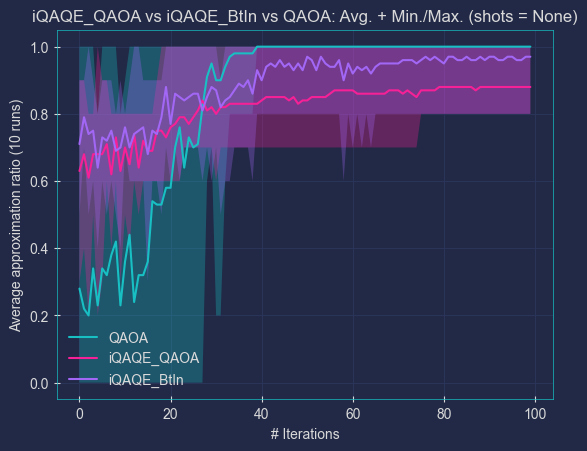
\includegraphics[width=0.60\textwidth]{Figures/Chapter_5/iQAQE_QAOA.png}
  \caption{Average approximation ratio ($\pm$ Min./Max.) \textit{vs.} iteration number, for the three tested \acrshort{vqa}\textcolor{gray}{s}: \texttt{QAOA}, \texttt{iQAQE\_QAOA} (as described above) and \texttt{iQAQE\_BtIn}. The latter stands for \acrshort{iqaqe}, with better initialization. This corresponds to the same mapping as the one in Figure \ref{fig:3_Comparison_shots}.}
  \label{fig:iQAQE_QAOA}
\end{figure}
\vspace{-4.0mm}
This realization led us to understand that we cannot expect to replicate \acrshort{qaoa}'s outstanding performance on this graph simply by using a \acrshort{qaoa}-type mapping. After all, we are still relying on \acrshort{qemc}'s cost function and ansatz, so this outcome is not entirely surprising. Moreover, to add to the challenge, we found that \texttt{iQAQE\_QAOA}'s performance can even be surpassed by another random, non-specific mapping, highlighting how far we are from achieving \acrshort{qaoa}-like results.

In an effort to bridge this gap, we attempted to integrate \acrshort{qaoa}'s ansatz into the scheme, alongside the \acrshort{qaoa}-type mapping. However, after extensive testing, we realized this approach is not feasible. Here's why: using both elements together with the node probability encoding (as a normalized sum of their associated basis states' probabilities) causes the \acrshort{qemc} cost function to become independent of the ansatz's parameters\footnote{To verify this, we performed analytical calculations for a simple toy model: a graph with two nodes connected by a single edge. The results generalize to larger graphs.}. This means we cannot proceed with training, rendering the scheme ineffective. Thus, implementing this approach in its current form is not possible. For it to be successful, other aspects would need to change, such as the cost function or the method of deriving node probabilities from basis states' probabilities, which is the main issue here.









%%%%%%%%%%%%%%%%%%%%%%%%%%%%%%%%%%%%%%%%%%%%%%%%%%%%%%%%%%%%%%%%%%%%%%%%
% \subsection{Parity-like QAOA}
% \label{subsection:Parity_QAOA}

% Parity-like QAOA schemes and their results.

% % Send this to Chapter 6, instead.





%%%%%%%%%%%%%%%%%%%%%%%%%%%%%%%%%%%%%%%%%%%%%%%%%%%%%%%%%%%%%%%%%%%%%%%%
\vspace{-5mm}
\subsection{Correlation-based iQAQE}
\label{subsection:Correlation_iQAQE}
\vspace{-2.5mm}
This scheme closely resembles what was previously discussed in subsection \ref{subsection:Basic_Poly-Comp_iQAQE}. The key distinction lies in the inclusion of the possibility for both $0$'s and $1$'s to be fixed (e.g., $\{\ket{11\text{xxx}}, \ket{00\text{xxx}}\}$, for $k = 2$; recall, this encodes a single node). Consequently, the scheme aims to identify correlations among the different qubits, wherein "correlations" denote identical colors. In other words, the constructed lists regard the $k$ fixed qubits as positively correlated, meaning they are either all set to $1$ or all set to $0$. This approach was inspired by the notion that by identifying correlations between nodes, it becomes feasible to color the entire graph as long as one node is initially colored. Although seeking correlations between qubits, as done here, differs from seeking correlations between nodes, we anticipated that it might yield promising results to some extent. In this scenario, the color of each node is determined by the probability that its $k$ associated qubits are all positively correlated.

To delve deeper into the properties and characteristics of this scheme, we conducted a thorough formal analysis, exploring its limits by considering scenarios where $k$ ranges from $1$ to $n$ qubits, covering the entire spectrum. Our primary objective was to ascertain if we could formulate this correlation-based \acrshort{iqaqe} scheme in a manner that truly interpolates between \acrshort{qaoa} and \acrshort{qemc}. We aimed to determine if we could retrieve both algorithms by adjusting the parameters accordingly. However, with this correlation-based scheme, we not only cannot recover \acrshort{qaoa}, but we also fail to retrieve \acrshort{qemc}. Thus, this does not represent an interpolation between the two algorithms. Likewise, earlier, we loosely referred to the \acrshort{iqaqe} Framework as an interpolation. However, upon closer scrutiny, this characterization seems inaccurate. While it is possible to recover the \acrshort{qemc} limit\footnote{Simply utilize the appropriate number of qubits and select one unique basis state for each node.}, the same cannot be said for \acrshort{qaoa}, as we have observed before. Additionally, we present the results of numerical simulations applied to the standard $8$-node graph using this correlation-based \acrshort{iqaqe} approach (Figure \ref{fig:Correlation-based}).

\begin{figure}[H]
  \centering
  \begin{subfigure}[t]{0.495\textwidth}
      \centering
      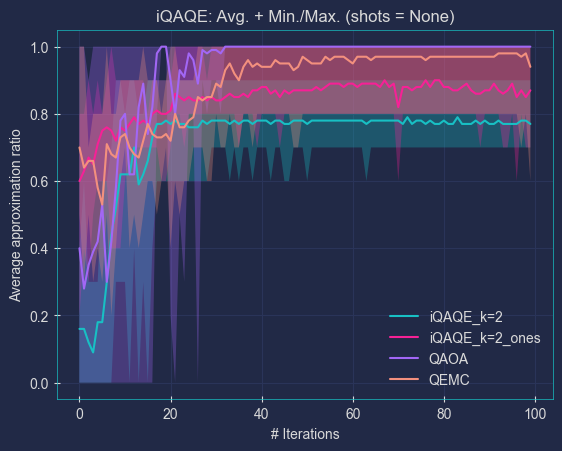
\includegraphics[width=\textwidth]{Figures/Chapter_5/Correlation-based/k=2(Reg.+Ones).png}
      \caption{\raggedright Comparison of Correlation-based \acrshort{iqaqe} for $k=2$ with results from \acrshort{qaoa}, \acrshort{qemc}, and the previous Basic Polynomial Compression-type iQAQE\footnotemark{} (\texttt{iQAQE\_k=2\_ones}).}
      \label{fig:Correlation/k=2}
  \end{subfigure}
  \hfill
  \begin{subfigure}[t]{0.495\textwidth}
      \centering
      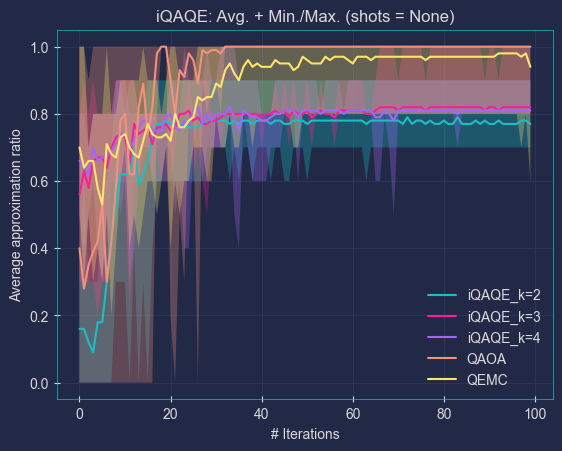
\includegraphics[width=\textwidth]{Figures/Chapter_5/Correlation-based/k=2_3_4.png}
      \caption{Comparison of Correlation-based \acrshort{iqaqe} results for $k=2, 3$, and $4$ with outcomes from \acrshort{qaoa} and \acrshort{qemc}.}
      \label{fig:Correlation/k=2,3,4}
  \end{subfigure}
  \caption{Correlation-based polynomial-type compression scheme ($k=2, 3$ and $4$): numerical simulations for the usual $8$-node graph.}
  \label{fig:Correlation-based}
\end{figure}

\clearpage

% This one is bugged. I don't know why, though. All the other ones are fine, I think.
\footnotetext[\value{footnote}]{This refers to the scenario where only $1$'s are fixed, not $0$'s.}

\begin{figure}[H]
  \centering
  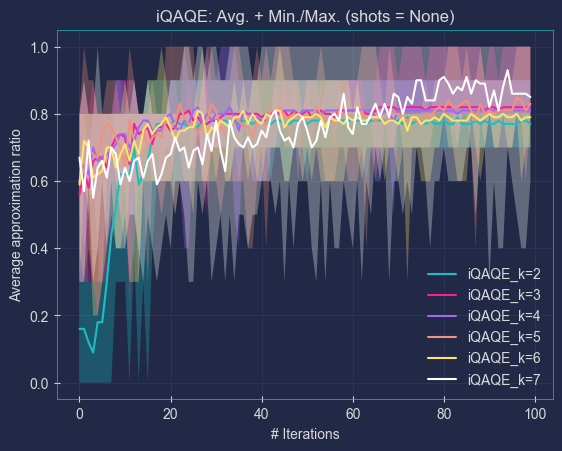
\includegraphics[width=\textwidth]{Figures/Chapter_5/Correlation-based/All_k's.png}
  \caption{Correlation-based polynomial-type compression scheme ($k = 2, 3, 4, 5, 6$ and $7$): numerical simulations for the usual $8$-node graph.}
  \label{fig:All_k's}
\end{figure}

Note that we once again compute the average approximation ratio from $10$ runs, each with different random initial parameters, and generate all curves with \texttt{n\_layers = 3} and \texttt{step\_size = 0.95}. Additionally, we plot the average, with the shaded region representing the maximum and minimum obtained approximation ratios (out of the $10$ runs). Performance-wise, this scheme does not fare well. It is significantly outperformed by \acrshort{qaoa}, \acrshort{qemc}, and the basic polynomial compression-type \acrshort{iqaqe}. We also compared the results for all possible values of $k$ (Figure \ref{fig:All_k's}). It turns out that the specific value of $k$ is not very meaningful, as performance is quite similar across all values.

The underperformance is likely due to our doubling the number of basis states in each sub-list. This encoding results in each pair of sub-lists having a $50\%$ overlap, similar to the Basic Polynomial Compression-type \acrshort{iqaqe}. However, with twice\footnote{Either $0$'s or $1$'s can be fixed.} the number of basis states this time, the number of overlapping basis states is significantly higher. This increase means that more states are shared by multiple nodes. When the overlap is too large, it becomes more challenging to adjust the color of one node without affecting the others. We believe this to be the main reason for the underperformance. We will be mindful of this in the design of future schemes.

% One of these schemes allowed to easily recover QEMC in one of its limits. Try to figure out what that was.

% Analytical analysis: do I even want to include this here? It didn't really amount to much, in the end... I'll have to think about this.





%%%%%%%%%%%%%%%%%%%%%%%%%%%%%%%%%%%%%%%%%%%%%%%%%%%%%%%%%%%%%%%%%%%%%%%%
\subsection{Fixed-Parity iQAQE}
\label{subsection:Fixed-Parity_iQAQE}

% Mention that this is a 'heuristic'. It's not a strict rule, but it's a good guideline.

In this section, we present another heuristic method for mapping the basis states to the nodes. Although it is similar to the previous one, this time we \textbf{fixed the parity of the selected $k$ qubits to be even}. Parity is determined by the number of $1$'s: if the count is even, the parity is even; otherwise, it is odd. For instance, for $k=3$ (with \texttt{n\_qubits = 5}), the lists would take the form: (Keep in mind that we are using an $8$-node graph. \text{x} denotes a free qubit: either $0$ or $1$.)

% Remeber that 'k=2' is the same as the previous correlation-based! Mention this in the text!

\begin{multicols}{2}
  \begin{enumerate}
    \item $\left\{\ket{000\text{xx}}, \ket{011\text{xx}}, \ket{101\text{xx}}, \ket{110\text{xx}}\right\}$;
    \item $\left\{\ket{00\text{xx}0}, \ket{01\text{xx}1}, \ket{10\text{xx}1}, \ket{11\text{xx}0}\right\}$;
    \item $\left\{\ket{0\text{xx}00}, \ket{0\text{xx}11}, \ket{1\text{xx}01}, \ket{1\text{xx}10}\right\}$;
    \item $\left\{\ket{\text{xx}000}, \ket{\text{xx}011}, \ket{\text{xx}101}, \ket{\text{xx}110}\right\}$;
    \item $\left\{\ket{\text{x}0\text{x}00}, \ket{\text{x}0\text{x}11}, \ket{\text{x}1\text{x}01}, \ket{\text{x}1\text{x}10}\right\}$;
    \item $\left\{\ket{\text{x}00\text{x}0}, \ket{\text{x}01\text{x}1}, \ket{\text{x}10\text{x}1}, \ket{\text{x}11\text{x}0}\right\}$;
    \item $\left\{\ket{\text{x}000\text{x}}, \ket{\text{x}011\text{x}}, \ket{\text{x}101\text{x}}, \ket{\text{x}110\text{x}}\right\}$;
    \item $\left\{\ket{0\text{x}0\text{x}0}, \ket{0\text{x}1\text{x}1}, \ket{1\text{x}0\text{x}1}, \ket{1\text{x}1\text{x}0}\right\}$.
  \end{enumerate}
\end{multicols}
\noindent Once again, numerical simulations were performed, and the obtained results are presented below (Figure \ref{fig:Fixed-parity}). Although the performance is still not quite on par with \acrshort{qaoa}, it is significantly better than in the previously considered scenario. Note that the case where $k=2$ corresponds to the previous correlation-based scheme. For $k=2$, requiring the pair to be even is equivalent to requiring them to be the same (either both $0$ or both $1$), which explains the similarity in results. This similarity is apparent in the less favorable outcomes shown for $k=2$ in Figure \ref{fig:Fixed-parity}, which qualitatively match those in Figures \ref{fig:Correlation-based} and \ref{fig:All_k's}. However, when we allow for $k>2$, the performance improves significantly, likely due to the reduced overlap between the basis states associated with different nodes.

A keen observer might notice that this scheme's results also allow for generating the \acrshort{maxcut} partition, as shown by the shaded pink region in Figure \ref{fig:Fixed-parity/k=2,3,4} for $k=3$. These shaded regions depict the maximum and minimum cuts achieved out of the $10$ runs. This reveals that, despite the greater variability and lower average performance than \acrshort{qaoa}, the algorithm can achieve the \acrshort{maxcut} partition in some runs. In practice, this is crucial. When running the algorithm $10$ times, our main interest is in the best outcome. This highlights the potential of this heuristic scheme.

\begin{figure}[hb!]
  \centering
  \begin{subfigure}[t]{0.495\textwidth}
      \centering
      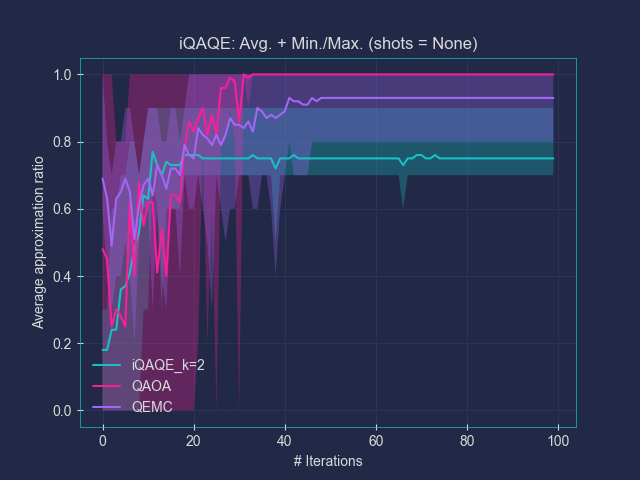
\includegraphics[width=1\textwidth]{Figures/Chapter_5/Fixed-parity/k=2(8-node).png}
      \caption{Fixed-parity \acrshort{iqaqe} for $k=2$ compared with the results from \acrshort{qaoa} and \acrshort{qemc} ($8$-node graph).}
      \label{fig:Fixed-parity/k=2}
  \end{subfigure}
  \hfill
  \begin{subfigure}[t]{0.495\textwidth}
      \centering
      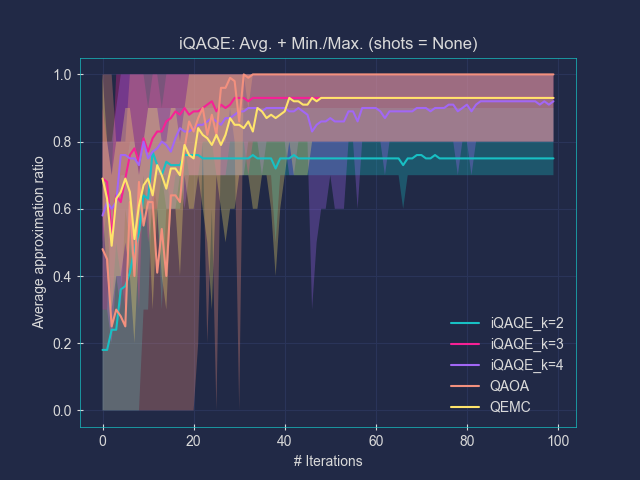
\includegraphics[width=1\textwidth]{Figures/Chapter_5/Fixed-parity/k=2_3_4(8-node).png}
      \caption{Fixed-parity \acrshort{iqaqe} for $k=2, 3$, and $4$ compared with the results from \acrshort{qaoa} and \acrshort{qemc} ($8$-node graph).}
      \label{fig:Fixed-parity/k=2,3,4}
  \end{subfigure}
\end{figure}

\clearpage

\begin{figure}[ht!]
  \addtocounter{figure}{-1} % Added <<
  \centering
  \begin{subfigure}[b]{1\textwidth}
      \addtocounter{subfigure}{2} % Added <<
      \centering
      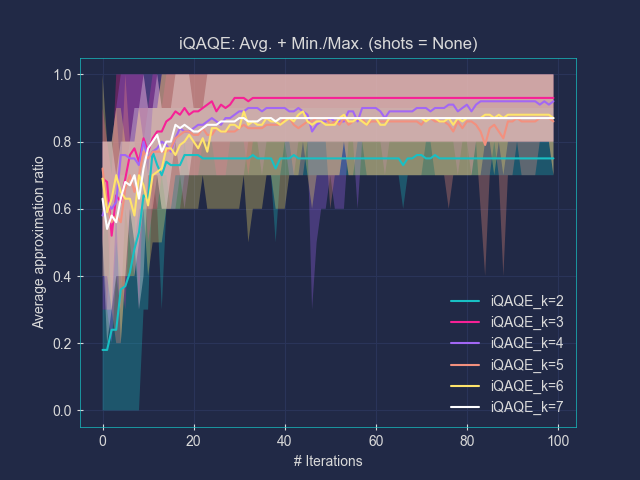
\includegraphics[width=1\textwidth]{Figures/Chapter_5/Fixed-parity/All_k's(8-node).png}
      \caption{Fixed-parity \acrshort{iqaqe} for all values of $k = 2, 3, 4, 5, 6$, and $7$ ($8$-node graph).}
      \label{fig:Fixed-parity/All_k's}
  \end{subfigure}
  \caption{Fixed-parity polynomial-type compression scheme: numerical simulations for the usual $8$-node graph. Please note that we utilize \texttt{n\_layers = 3}, \texttt{step\_size = 0.95} and \texttt{B = 4}.}
  \label{fig:Fixed-parity}
\end{figure}

Furthermore, numerical simulations were carried out on a random $16$-node graph\footnote{This graph was generated using NetworkX's \texttt{nx.gnm\_random\_graph(n, m)} with \texttt{n = 16} nodes and \texttt{m = 32} edges, using \texttt{np.random.seed} set to \texttt{44}.}. Considering the satisfactory performance observed with the previous $8$-node graph, we were interested in assessing the algorithm's performance on a larger scale. The results are now presented (Figure \ref{fig:Fixed-parity(16_node)}).

\begin{figure*}[ht!]
  \centering
  \begin{subfigure}[t]{0.495\textwidth}
      \centering
      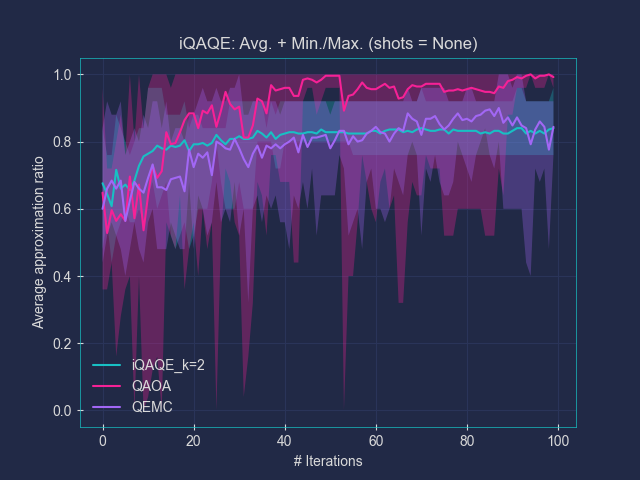
\includegraphics[width=1\textwidth]{Figures/Chapter_5/Fixed-parity/k=2(16-node).png}
      \caption{Fixed-parity \acrshort{iqaqe} for $k=2$ compared with the results from \acrshort{qaoa} and \acrshort{qemc} ($16$-node graph).}
      \label{fig:Fixed-parity/k=2(16_node)}
  \end{subfigure}
  \hfill
  \begin{subfigure}[t]{0.495\textwidth}
      \centering
      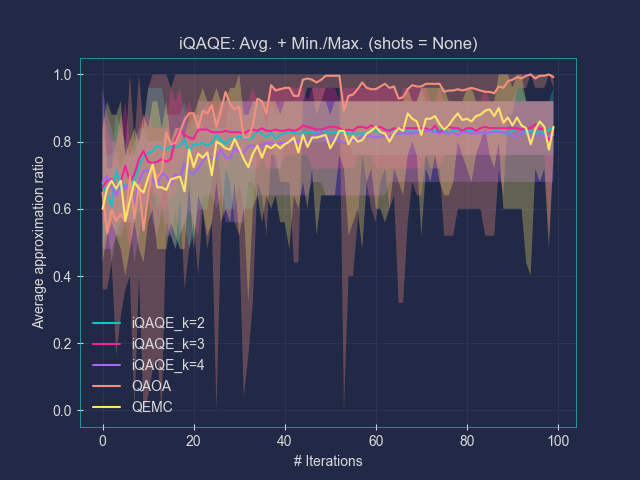
\includegraphics[width=1\textwidth]{Figures/Chapter_5/Fixed-parity/k=2_3_4(16-node).png}
      \caption{Fixed-parity \acrshort{iqaqe} for $k=2, 3$, and $4$ compared with the results from \acrshort{qaoa} and \acrshort{qemc} ($16$-node graph).}
      \label{fig:Fixed-parity/k=2,3,4(16_node)}
  \end{subfigure}
\end{figure*}

\clearpage

\begin{figure*}[ht!]
  \addtocounter{figure}{-1} % Added <<
  \centering
  \begin{subfigure}[b]{\textwidth}
      \addtocounter{subfigure}{2} % Added <<
      \centering
      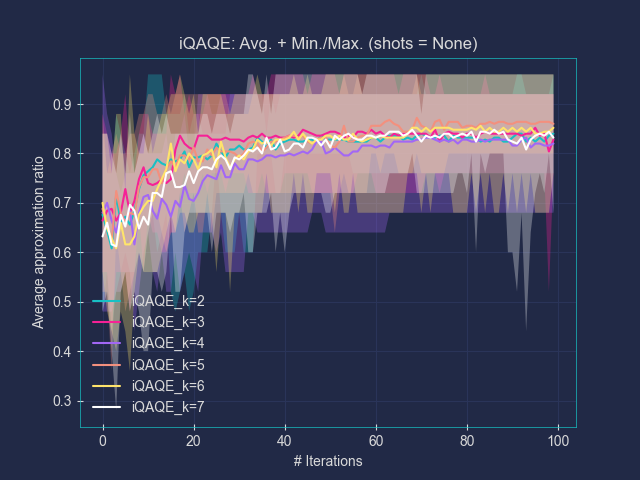
\includegraphics[width=1\textwidth]{Figures/Chapter_5/Fixed-parity/All_k's(16-node).png}
      \caption{Fixed-parity \acrshort{iqaqe} for all values of $k = 2, 3, 4, 5, 6$, and $7$ ($16$-node graph).}
      \label{fig:All_k's(16_node)}
  \end{subfigure}
  \caption{Fixed-parity polynomial-type compression scheme: numerical simulations for a $16$-node graph. Please note that we utilize \texttt{n\_layers = 3}, \texttt{step\_size = 0.95} and \texttt{B = 8}.}
  \label{fig:Fixed-parity(16_node)}
\end{figure*}

The previously identified trends are also apparent here. However, the performance now seems insufficient to achieve the \acrshort{maxcut} partition (determined by brute-force), as illustrated by the shaded areas in Figure \ref{fig:All_k's(16_node)}: the maximum \acrshort{ar} never quite reaches $1$. Moreover, for this graph, varying the value of $k$ does not significantly impact performance. Hence, it is advisable to choose the value of $k$ that requires the fewest qubits. In this instance, $k=3$ is optimal, needing only \texttt{n\_qubits = 6}, since $\binom{6}{3} = 20 \geq 16$.

%%%%%%%%%%%%%%%%%%%%%%%%%%%%%%%%%%%%%%%%%%%%%%%%%%%%%%%%%%%%%%%%%%%%%%%%
% \section{Other Exploratory Ideas}
% \label{section:Exploratory_Ideas}

% Other exploratory ideas and their results.

% % Send this to Chapter 6, instead.




%%%%%%%%%%%%%%%%%%%%%%%%%%%%%%%%%%%%%%%%%%%%%%%%%%%%%%%%%%%%%%%%%%%%%%%%
% \subsection{Tranche-based Oracle colouring}
% \label{section:Oracle_colouring}

% Tranche-based Oracle colouring schemes and their results.

% % Send this to Chapter 6, instead.




%%%%%%%%%%%%%%%%%%%%%%%%%%%%%%%%%%%%%%%%%%%%%%%%%%%%%%%%%%%%%%%%%%%%%%%%
\section{Extended-QEMC}
\label{section:Extended_QEMC}

% Extended-QEMC scheme and variations thereof, and their results.

Amid the various schemes we've attempted, I've devised an extension to the standard \acrshort{qemc} scheme. This new approach enhances \acrshort{qemc} by incorporating $m$ additional qubits beyond the usual $\lceil\log_2(n)\rceil$ qubits required for $n$ graph nodes.

%%%%%%%%%%%%%%%%%%%%%%%%%%%%%%%%%%%%%%%%%%%%%%%%%%%%%%%%%%%%%%%%%%%%%%%%
\subsection{Unmodified Extended-QEMC}
\label{subsection:Vanilla_Extended_QEMC}

Rather than associating a single basis state with each graph node, this scheme assigns $2^m$ basis states per node. Importantly, similar to \acrshort{qemc}, the sets of basis states associated with different nodes do not overlap. This non-overlapping property is crucial, as we suspect that significant overlap between nodes' lists might contribute to the subpar performance observed in the correlation-based and fixed-parity ($16$-node graph) \acrshort{iqaqe}\textcolor{gray}{s}.

This extended scheme can be implemented within the \acrshort{iqaqe} formalism by using appropriate sub-lists of basis states. The assignment of states to each list is currently arbitrary; for simplicity, we use a straightforward partition: the first $2^m$ basis states go to the first list, the next $2^m$ to the second list, and so on (referred to as Unmodified Extended-\acrshort{qemc}). However, there may be a more optimal method for distributing these states that we have not explored here.

Additionally, it is important to note that Extended-\acrshort{qemc} requires more qubits than regular \acrshort{qemc}. This increase in qubits prevents the scheme from being easily classically simulable and allows for more basis states to be associated with each graph node. Consequently, this should provide more variables to manipulate, potentially improving our chances of finding a good solution.

Now, I present the results of applying this scheme to the usual $8$-node graph (Figure \ref{fig:Vanilla_Extended-QEMC}).
\begin{figure}[h]
    \centering
    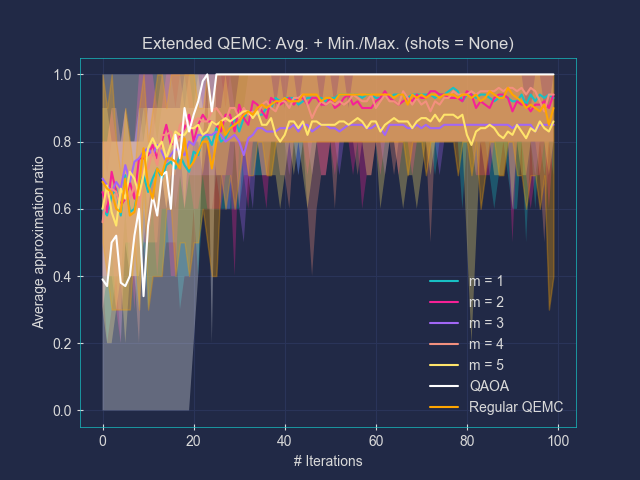
\includegraphics[width=0.95\textwidth]{Figures/Chapter_5/Extended-QEMC/8-node(n_layers=3, step_size=0.95, m=All).png}
    \caption{Implementation of the Unmodified Extended-\acrshort{qemc} scheme for the usual $8$-node graph: comparison with \acrshort{qaoa} and regular \acrshort{qemc} for various values of $m$. Note that $m$ is not extended beyond $5$, as this would exceed the number of qubits used in \acrshort{qaoa}. Additionally, we utilize \texttt{n\_layers = 3}, \texttt{step\_size = 0.95} and \texttt{B = 4}.}
    \label{fig:Vanilla_Extended-QEMC}
\end{figure}

\noindent As shown in this figure, the performance of the Unmodified Extended-\acrshort{qemc} scheme is qualitatively very similar to that of regular \acrshort{qemc}. For some values of $m$, we achieve slightly better results, but these improvements are not particularly significant. After conducting several tests, I found no clear pattern to predict which values of $m$ would yield the best results, supporting the earlier conclusion. Therefore, this presents another heuristic for mapping the basis states, with performance comparable to the standard \acrshort{qemc} scheme. While this is a satisfactory outcome, it is not particularly remarkable.

%%%%%%%%%%%%%%%%%%%%%%%%%%%%%%%%%%%%%%%%%%%%%%%%%%%%%%%%%%%%%%%%%%%%%%%%
\protect\subsection{Cardinality \texorpdfstring{$= 1$}{= 1} Extended-QEMC}
\label{subsection:Card._eq_1_Extended_QEMC}

Motivated by the results in Figure \ref{fig:seed=13}\footnote{The trajectory of this study was far from linear. The results presented here are not in the chronological order of our research, hence this reference to later work, which was actually conducted before devising the Extended-\acrshort{qemc} scheme.}, I decided to make a slight change to the Unmodified Extended-\acrshort{qemc} scheme: instead of assigning $2^m$ basis states to each node, we assign only one basis state (randomly) to each node (Cardinality $= 1$ Extended-\acrshort{qemc}). Although this adjustment occasionally yielded marginally better results than regular \acrshort{qemc}, we do not consider these improvements significant (see Figure \ref{fig:Card.=1_Extended-QEMC} for reference).
\begin{figure}[h]
    \centering
    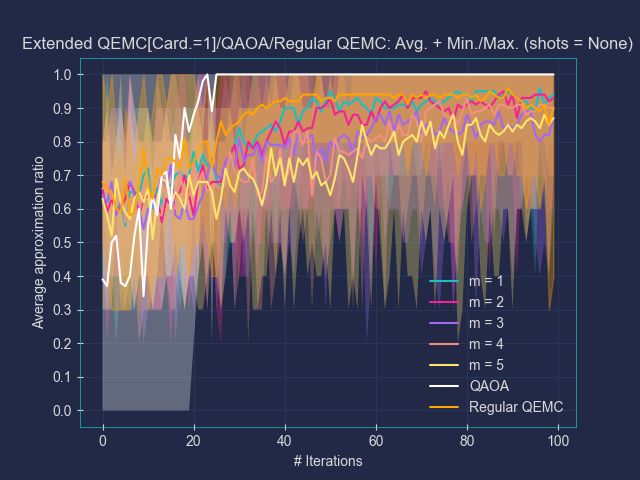
\includegraphics[width=1\textwidth]{Figures/Chapter_5/Extended-QEMC/8-node[Card.=1](n_layers=3, step_size=0.95, m=All).png}
    \caption{Implementation of the Cardinality $= 1$ Extended-\acrshort{qemc} scheme for the standard $8$-node graph: comparison with \acrshort{qaoa} and regular \acrshort{qemc} for various values of $m$. Please note that we utilize \texttt{n\_layers = 3}, \texttt{step\_size = 0.95} and \texttt{B = 4}.}
    \label{fig:Card.=1_Extended-QEMC}
\end{figure}

%%%%%%%%%%%%%%%%%%%%%%%%%%%%%%%%%%%%%%%%%%%%%%%%%%%%%%%%%%%%%%%%%%%%%%%%
\vspace*{-1cm}
\section{Alternative ansätze}
\label{section:Alternative_ansätze}

After some reflection, I began to question whether the performance of \acrshort{qemc} and \acrshort{iqaqe} could be hindered by the use of a problem-agnostic ansatz. It's generally advantageous to incorporate problem-specific information into the ansatz, as exemplified by problem-inspired ansätze. Additionally, I pondered whether excessive entanglement or correlations among the system's basis states might be affecting the schemes' performances. Such phenomena could make it challenging for the model to adjust the amplitude of a specific basis state without significantly impacting others. To address this potential issue, the concept of implementing non-deterministic CNOT gates (\acrshort{ndcnot}\textcolor{gray}{s}) occurred to me\footnote{We recognize that the term "non-deterministic CNOT gates" is employed in linear optical quantum computing (KLM protocol), yet we use it differently in this context.}. This approach would allow the model to dynamically adjust the degree of entanglement. The most rudimentary way to implement this is by employing parameterized $R_x$ gates before each CNOT's control qubit, which is precisely what we did. The $R_x$ gate allows the control qubit to rotate in and out of the $\ket{1}$ state, thus adjusting the degree of entanglement introduced by the CNOT gate. The results for the standard $8$-node graph are presented below (Figure \ref{fig:ND-CNOTs}), for both \acrshort{qemc} and Cardinality $= 1$ Extended-\acrshort{qemc}.
\begin{figure}[h]
  \centering
  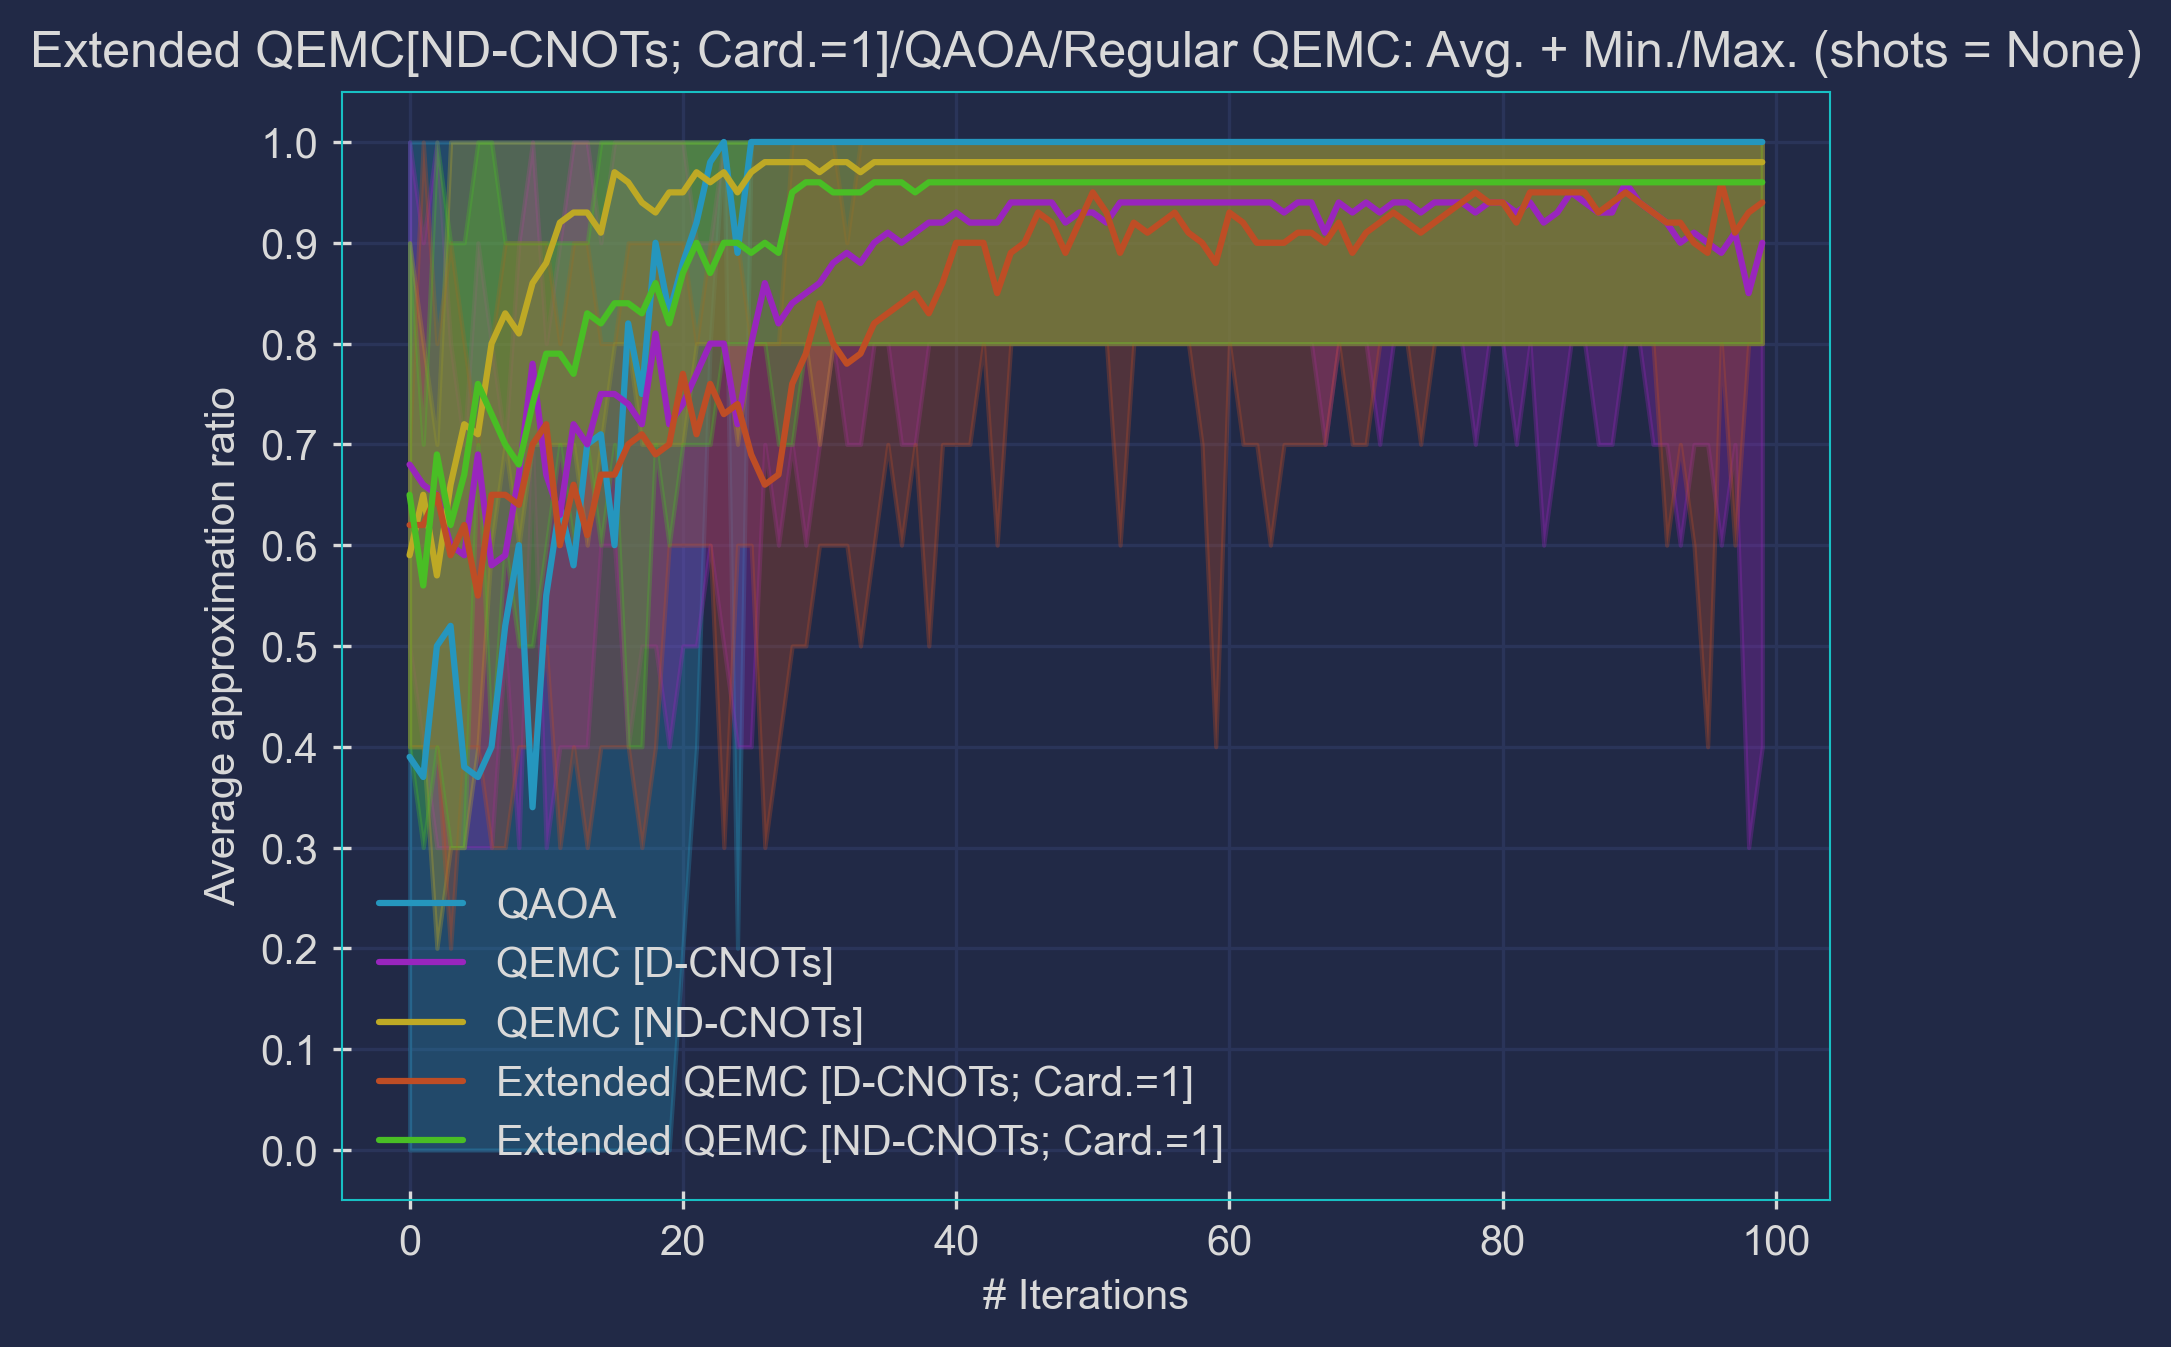
\includegraphics[width=1.0\textwidth]{Figures/Chapter_5/Extended-QEMC/8-node[ND-CNOTs; Card.=1](n_layers=2, step_size=0.5).png}
  \caption{Comparison of \acrshort{qemc} and Extended-\acrshort{qemc} implementations utilizing both \acrshort{dcnot}\textcolor{gray}{s} and \acrshort{ndcnot}\textcolor{gray}{s} for the usual $8$-node graph, alongside \acrshort{qaoa}. Keep in mind that we utilize \texttt{B = 4}.}
  \label{fig:ND-CNOTs}
\end{figure}

Several noteworthy observations can be made here. Firstly, it's apparent that \acrshort{ndcnot}-based schemes exhibit significantly more stable performance with fewer fluctuations compared to deterministic CNOT-based (\acrshort{dcnot}) schemes. This discrepancy arises from differences in their implementations: \acrshort{dcnot} circuits employ \texttt{n\_layers = 3} and \texttt{step\_size = 0.95} (Adam's learning rate), whereas \acrshort{ndcnot} circuits use \texttt{n\_layers = 2} and \texttt{step\_size = 0.5}. The latter, \texttt{step\_size = 0.5}, accounts for the smoother curves observed in Figure \ref{fig:ND-CNOTs}, as expected, and may also contribute to faster convergence. Secondly, the performance appears noticeably enhanced when utilizing \acrshort{ndcnot}\textcolor{gray}{s}, particularly evident in the case of regular \acrshort{qemc}: a distinct improvement is evident when comparing the yellow and purple lines. Despite introducing added complexity to the optimization landscape, this approach appears to yield significant performance gains, at least for this small $8$-node graph. Thus, we've proposed a novel scheme that builds upon \acrshort{qemc}, showing great potential to outperform it.

Moreover, this analysis serves to validate the notion that deviating from purely problem-agnostic ansätze is generally beneficial. This insight will inform our approach in developing future schemes in subsequent research endeavors. Encouraged by the promising outcomes from this study, we opted to expand the testing of this scheme to larger graphs to assess its scalability. This paves the way for comparisons with the Goemans-Williamson algorithm.





%%%%%%%%%%%%%%%%%%%%%%%%%%%%%%%%%%%%%%%%%%%%%%%%%%%%%%%%%%%%%%%%%%%%%%%%
\vspace{-2.5mm}
\section{Goemans-Williamson and Bigger Graphs}
\label{section:GW_Bigger_Graphs}

% I have finally fixed the graphs! However, I might now need to sligthly adjust the text to better fit the new graphs. I can re-introduce the previous text here ("Better than G-W [...]").

At one point, I began to question whether it was appropriate to directly compare our results to \acrshort{qaoa}, which stands out as the best-performing \acrshort{vqa} among those tested. After thorough deliberation, we concluded that, indeed, it makes sense to do so for smaller graphs. However, as graphs increase in size, the availability of quantum machines with a necessary number of qubits to support such \acrshort{qaoa}\textcolor{gray}{s} becomes limited. This circumstance has led to the emergence of schemes like \acrshort{qemc} \cite{tenecohen2023variational} and others \cite{sciorilli2024largescale}, which aim to address the limitations imposed by the number of qubits.

In light of this, I proceeded to evaluate the performance of our proposed schemes on larger graphs. Two such graphs were considered:
\begin{enumerate}
    \item $32$-node Erdős–Rényi graph, constructed using NetworkX's {\hypersetup{urlcolor=black}\url{nx.erdos\_renyi\_graph(n = 32, p = 0.2, seed=0, directed=False)}}, where each edge is included in the graph with a probability of $p = 0.2$;
    \item $100$-node Erdős–Rényi graph, defined similarly to the previous graph, utilizing {\hypersetup{urlcolor=black}\url{nx.erdos\_renyi\_graph(n = 100, p = 0.2, seed=0, directed=False)}}.
\end{enumerate}
The results obtained from these evaluations are presented below\footnote{Please note that we have included only the most promising schemes.} (Figures \ref{fig:32-node_Graph(2-Subfigures)} and \ref{fig:100-node_Graph(2-Subfigures)}).

\begin{figure*}[hb!]
    \centering
    \begin{subfigure}[b]{0.495\textwidth}
        \centering
        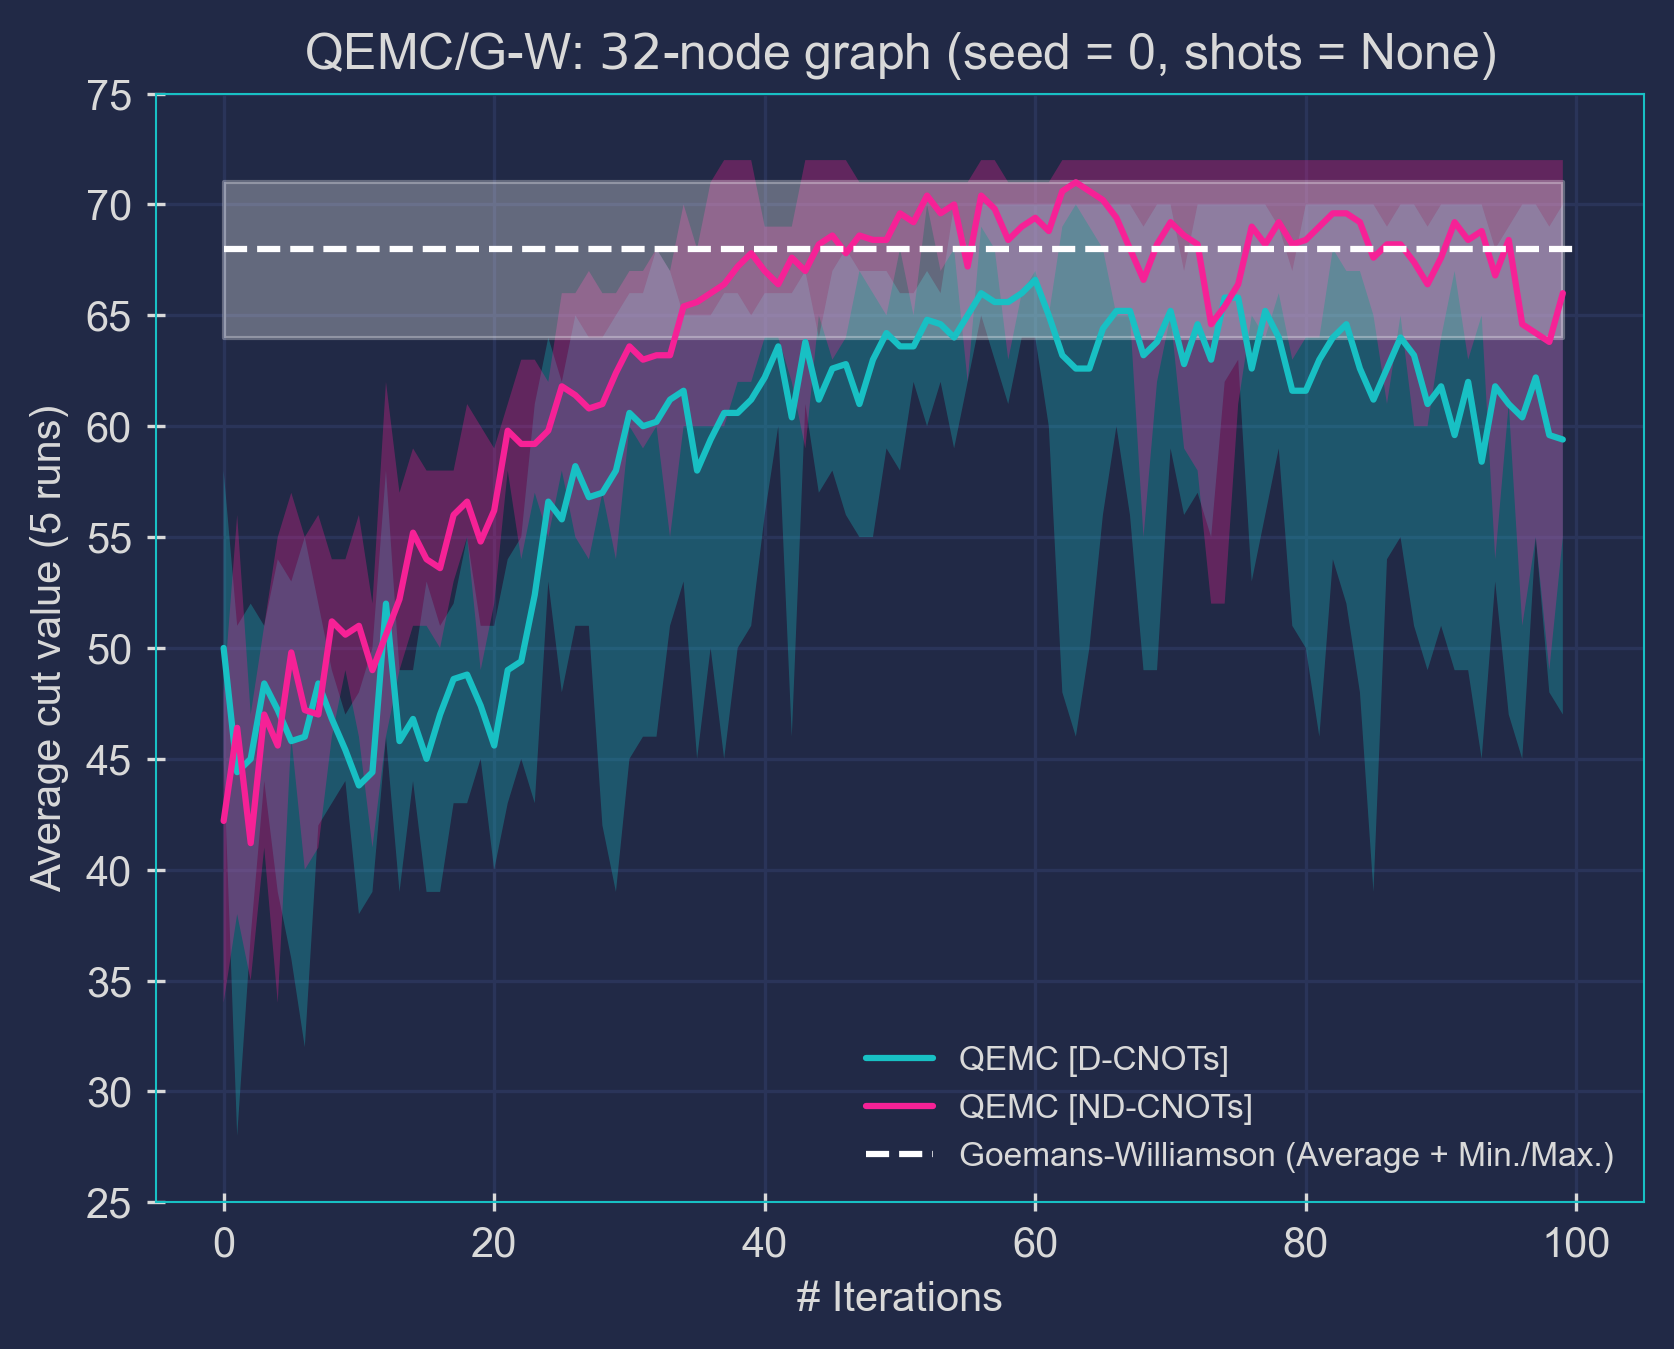
\includegraphics[width=1\textwidth, height=0.812\textwidth]{Figures/Chapter_5/Large graphs/32-node_Graph(QEMC&G-W)_seed=0.png}
        \caption{$32$-node graph – \acrshort{qemc} and \acrshort{gw} exclusively.}
        \label{fig:32-node_Graph(QEMC&G-W)}
    \end{subfigure}
    \hfill
    \begin{subfigure}[b]{0.495\textwidth}
        \centering
        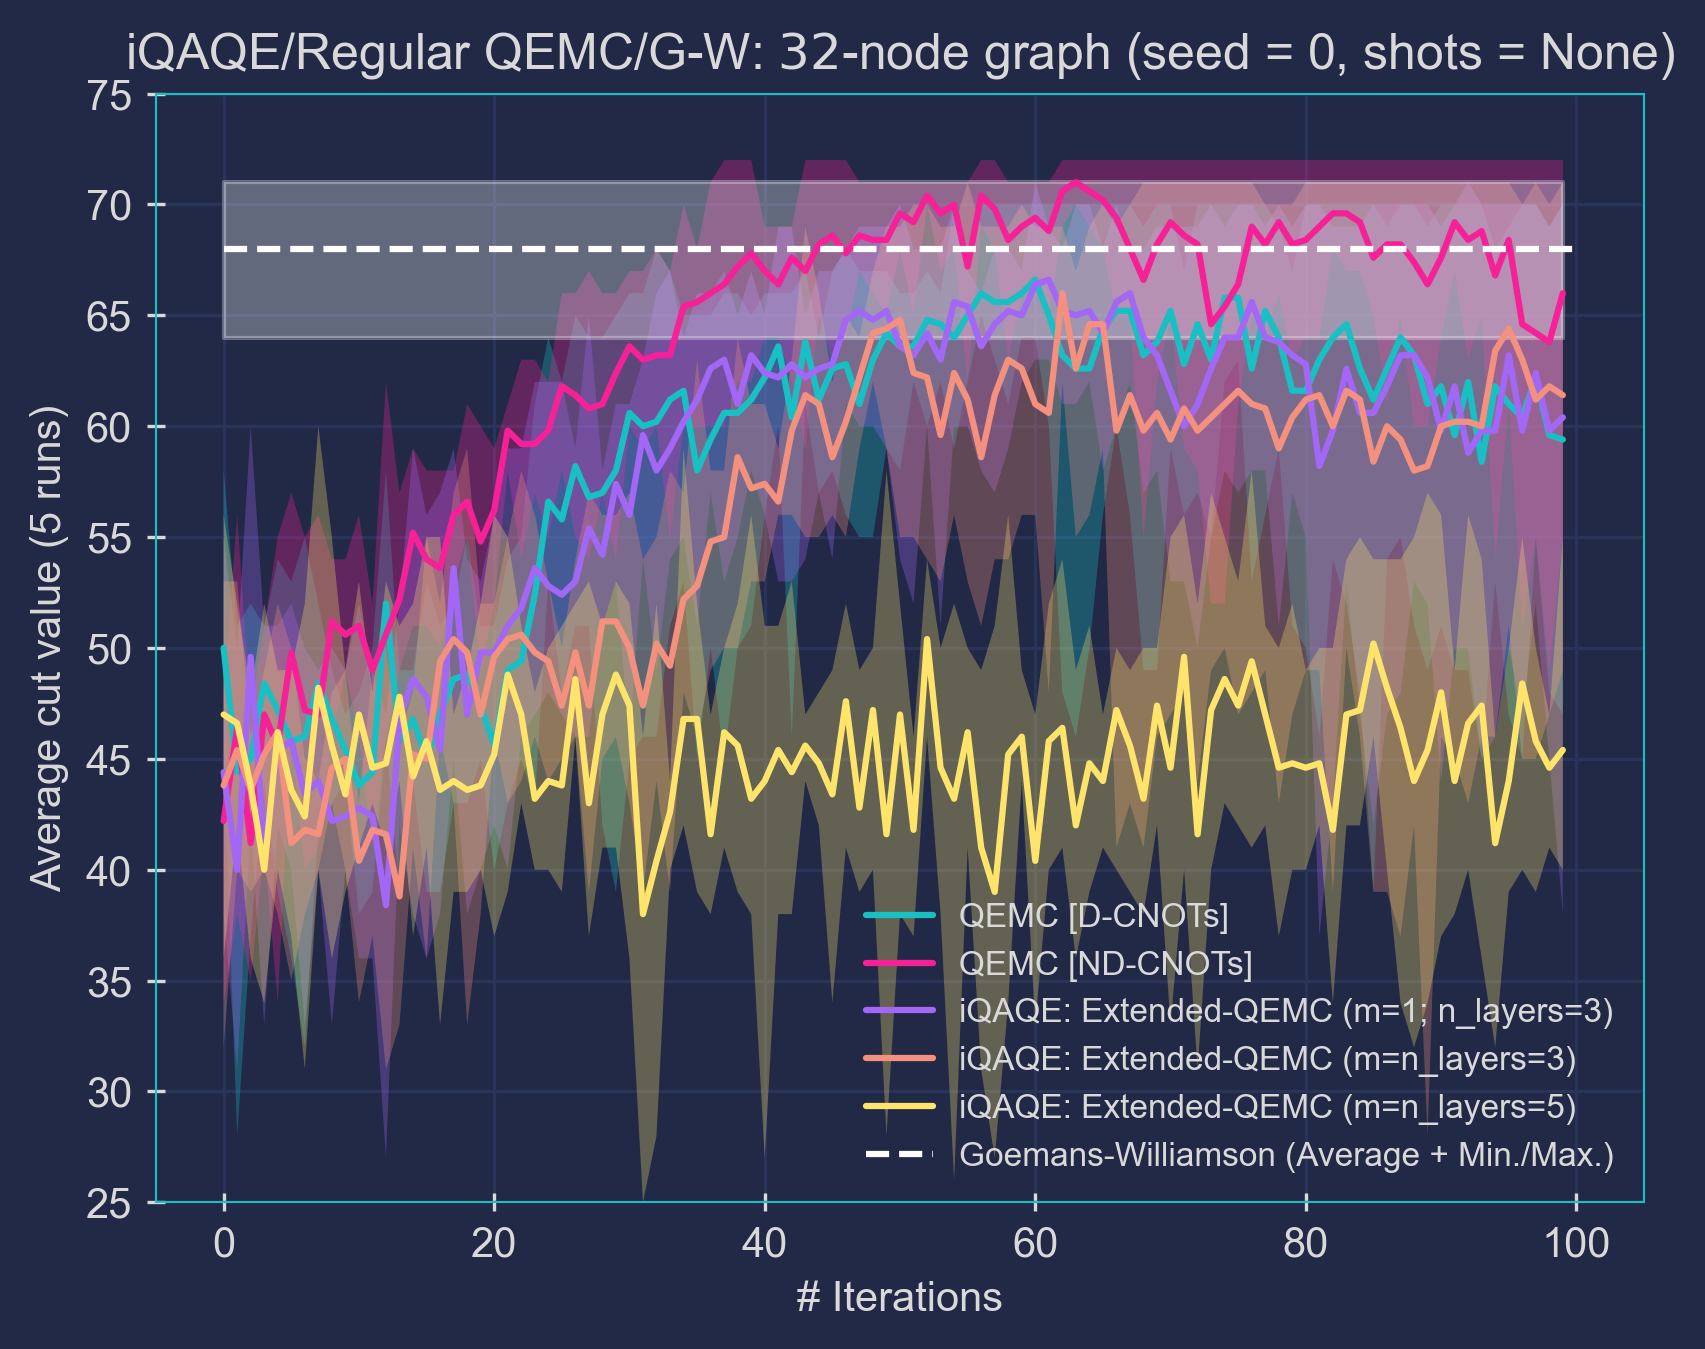
\includegraphics[width=1\textwidth, height=0.812\textwidth]{Figures/Chapter_5/Large graphs/32-node_Graph_seed=0.png}
        \caption{$32$-node graph – other schemes.}
        \label{fig:32-node_Graph}
    \end{subfigure}
    \caption{Comparison of performance (average cut values) among various \acrshort{vqa} schemes for the specified $32$-node graph. \texttt{n\_layers = 3} was employed for both \acrshort{qemc}\textcolor{gray}{s}, with \texttt{step\_size = 0.95} for \acrshort{dcnot}-\acrshort{qemc} and \texttt{step\_size = 0.5} for \acrshort{ndcnot}-\acrshort{qemc}. For all Extended-\acrshort{qemc} schemes, \texttt{step\_size = 0.95} was utilized, with the number of layers specified in the legend. Keep in mind that we utilize \texttt{B = 16}.}
    \label{fig:32-node_Graph(2-Subfigures)}
\end{figure*}

\clearpage

\begin{figure*}[hb!]
    \centering
    \begin{subfigure}[b]{0.495\textwidth}
        \centering
        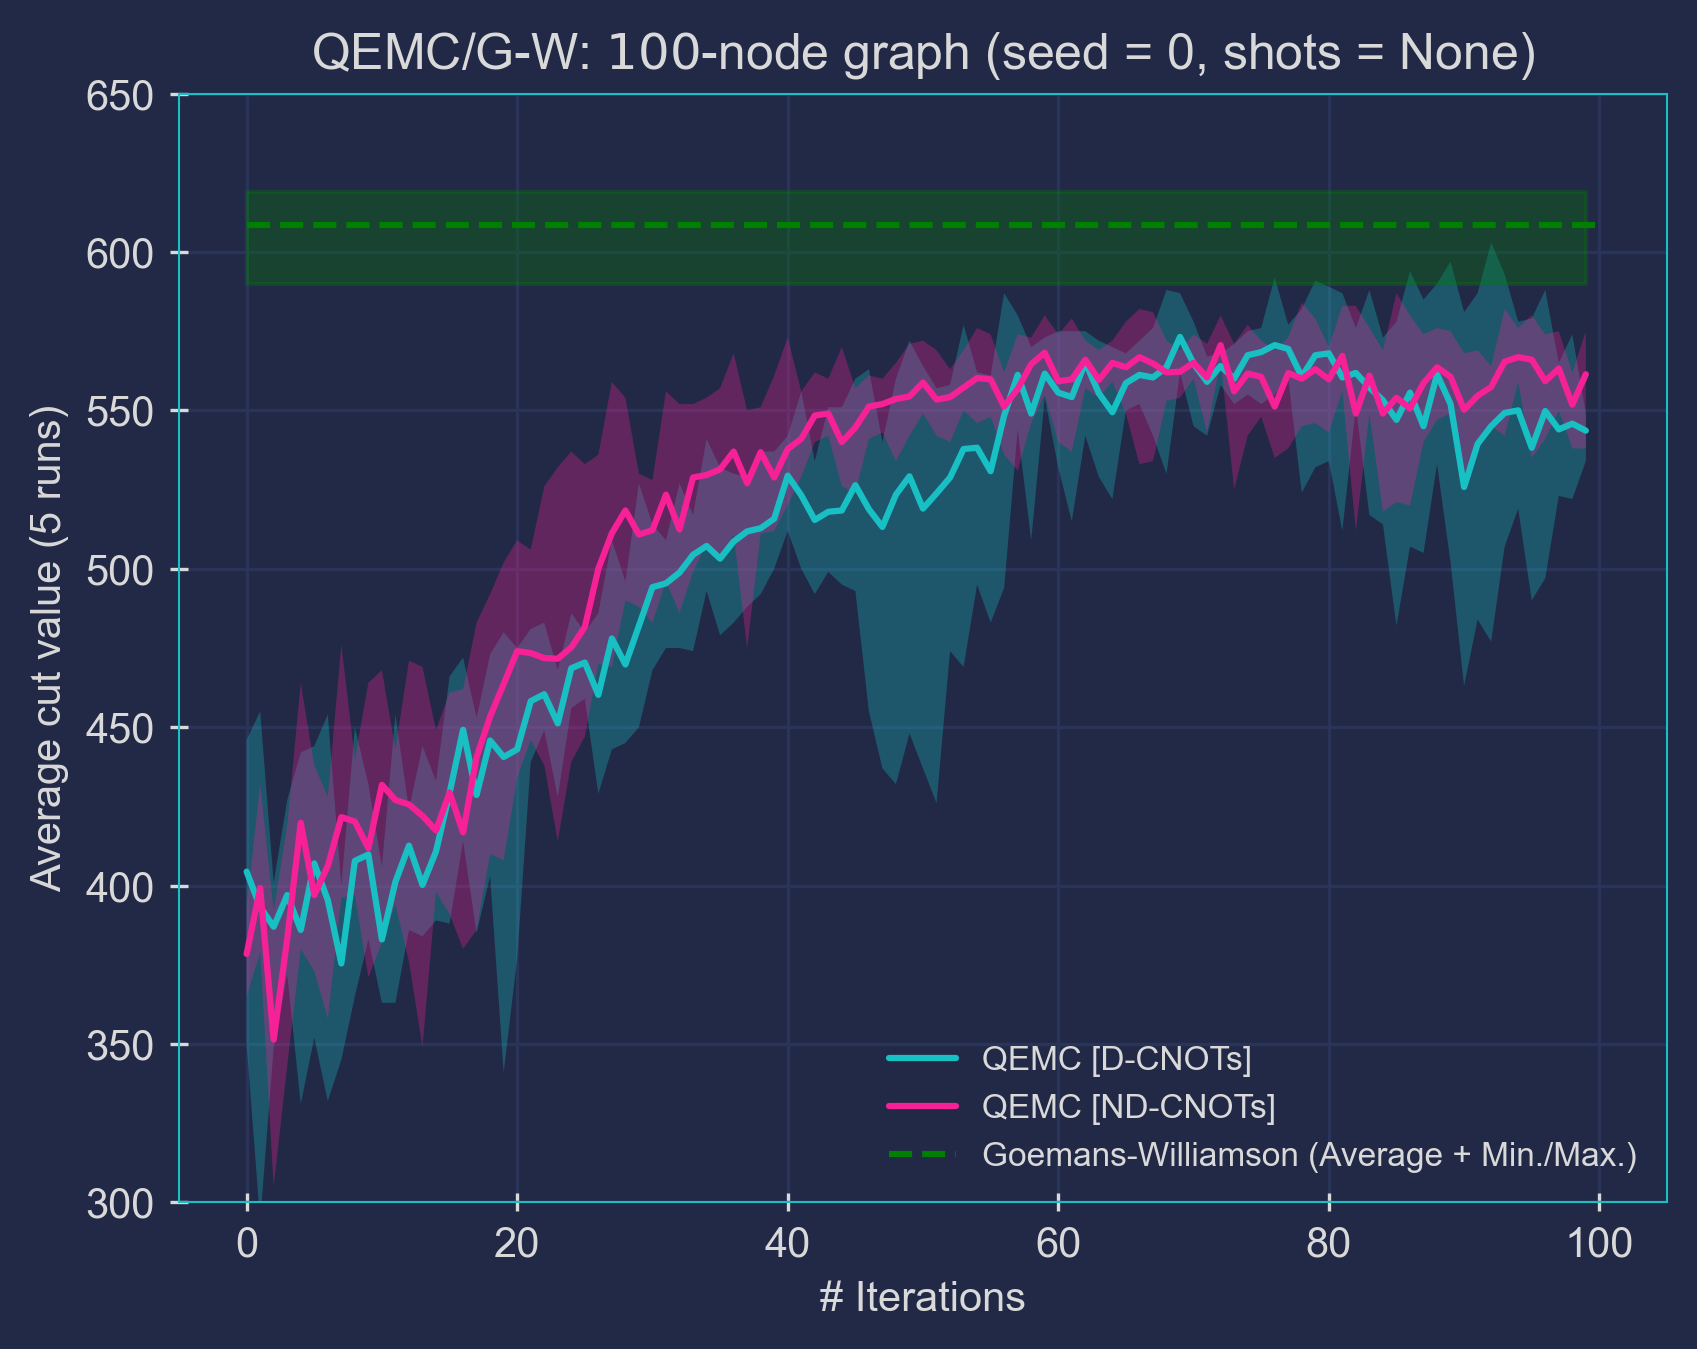
\includegraphics[width=1\textwidth, height=0.812\textwidth]{Figures/Chapter_5/Large graphs/100-node_Graph(QEMC&G-W)_seed=0.png}
        \caption{$100$-node graph – \acrshort{qemc} and \acrshort{gw} exclusively.}
        \label{fig:100-node_Graph(QEMC&G-W)}
    \end{subfigure}
    \hfill
    \begin{subfigure}[b]{0.495\textwidth}
        \centering
        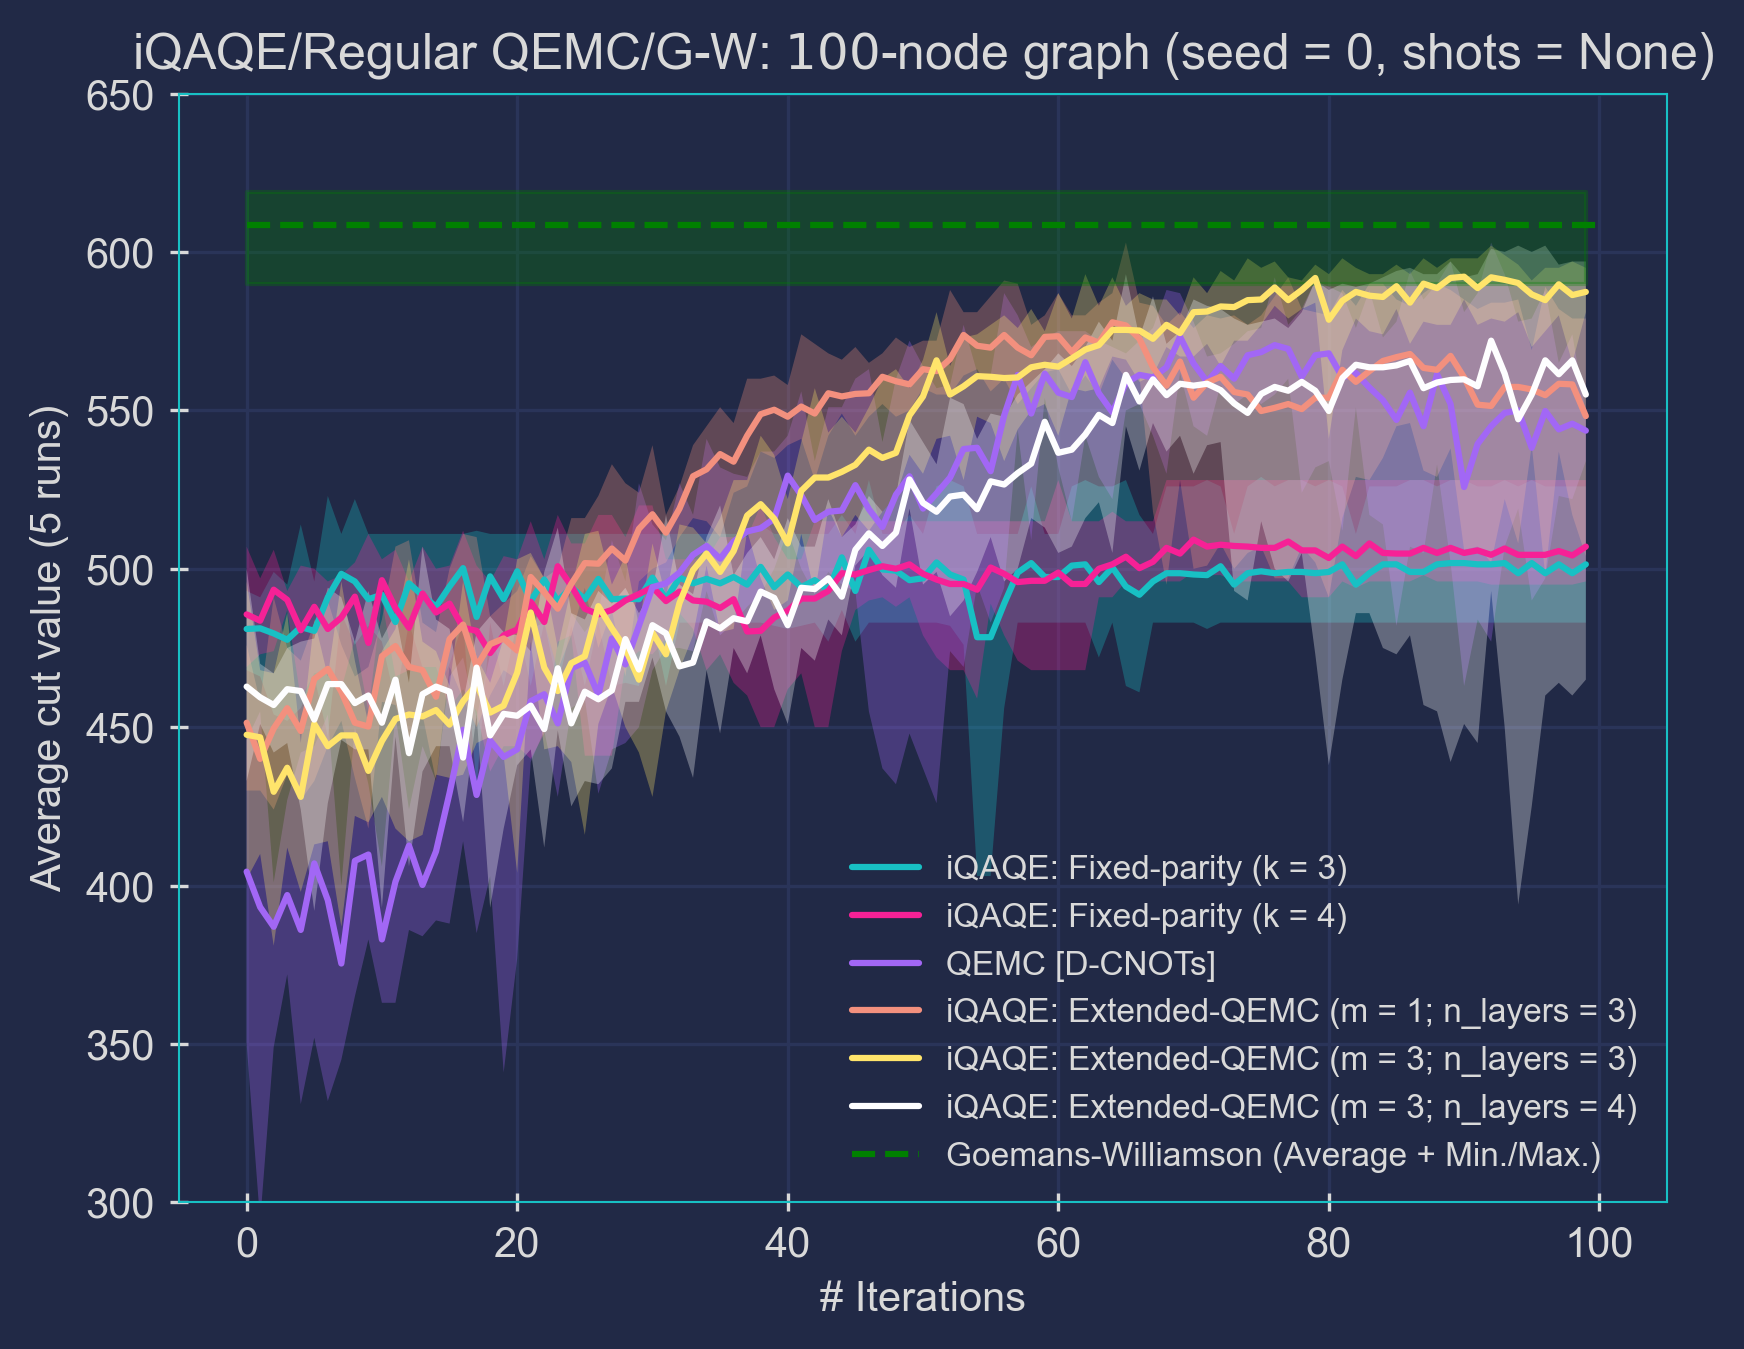
\includegraphics[width=1\textwidth, height=0.812\textwidth]{Figures/Chapter_5/Large graphs/100-node_Graph_seed=0.png}
        \caption{$100$-node graph – other schemes.}
        \label{fig:100-node_Graph}
    \end{subfigure}
    \caption{Comparison of performance (average cut values) among various \acrshort{vqa} schemes for the specified $100$-node graph. This time, all considered VQAs utilized \texttt{n\_layers = 3} and \texttt{step\_size = 0.95}, except for Extended-\acrshort{qemc} with $m=3$, which used \texttt{n\_layers = 4}. Keep in mind that we utilize \texttt{B = 50}.}
    \label{fig:100-node_Graph(2-Subfigures)}
\end{figure*}
% Notice how I added Fixed-parity iQAQE to Fig. 5.16 (b). Say this in the text, somewhere.

% I need to re-read this part, and change things to match the new results.

% Re-read this part!
% Old.
% In Figure \ref{fig:100-node_Graph(2-Subfigures)}, note that \acrshort{qemc}, fixed-parity \acrshort{iqaqe}, and \acrshort{gw} employ $10$ runs for averaging, while all other schemes (including Cardinality $= 1$ Extended-\acrshort{qemc}) use only $5$ runs. This decision was made to expedite the process while ensuring reasonable averaging of statistical fluctuations in the results. Likewise, in Figure \ref{fig:32-node_Graph(2-Subfigures)}, only $3$ runs were utilized for all schemes. Additionally, in Figure \ref{fig:100-node_Graph}, I chose to include the fixed-parity \acrshort{iqaqe} scheme to evaluate its performance on a larger graph.

% New.
Please note that we averaged the results over $5$ runs instead of the typical $10$. This adjustment was made to expedite the process while still achieving a reasonable averaging of statistical fluctuations. Additionally, in Figure \ref{fig:100-node_Graph}, I included the fixed-parity \acrshort{iqaqe} scheme to assess its performance on a larger graph.

% Re-read this part! Check if there's anything else that could be added to the analysis.
Now, concerning the results, several interesting observations emerge. For the $32$-node graph, Extended-\acrshort{qemc}'s performance varies considerably with different values of $m$ and \texttt{n\_layers}, as previously observed, making it inconsistent and challenging to optimize for other graphs. Once again, we observe the benefits of using \acrshort{ndcnot}\textcolor{gray}{s} in \acrshort{qemc} compared to the usual \acrshort{dcnot}\textcolor{gray}{s}. One might also observe that the average performance of the \acrshort{ndcnot}-based \acrshort{qemc} is highly competitive with \acrshort{gw}, occasionally even outperforming it. Furthermore, the maximum performance achieved by the \acrshort{ndcnot}-based scheme surpasses that of \acrshort{gw}, as evident from the comparison of the shaded pink and white regions (Figure \ref{fig:32-node_Graph(QEMC&G-W)}). This marks the first instance in this study where one of our heuristics surpasses classical state-of-the-art algorithms, representing a significant milestone and underscoring the potential for further exploration of the proposed \acrshort{iqaqe} Framework.

% This demonstrates that our heuristics can rival the state-of-the-art, marking a significant milestone and highlighting the potential for further exploration of the proposed \acrshort{iqaqe} Framework.

% I need to re-read/change this! Mention that ND-QEMC is no longer king! And, its performance becomes very similar to regular QEMC's.

% New.
Turning to the $100$-node graph, the situation differs somewhat. This time, the Extended-\acrshort{qemc} scheme stands out, delivering remarkable performance competitive with \acrshort{gw}. Additionally, we found that the previously mentioned fixed-parity \acrshort{iqaqe} performs exceptionally poorly, demonstrating its inability to generalize to larger graphs. Moreover, there is no longer a significant performance gap between the \acrshort{ndcnot}-based and regular \acrshort{qemc} schemes, suggesting that the former doesn't scale well to larger graphs. Nevertheless, for this $100$-node graph, reaching the average performance level of the Goemans-Williamson algorithm remains elusive, indicating ample room for improvement. However, once again, promising results are evident in the maximum cuts (shaded regions).

% % Old.
% Turning to the $100$-node graph, we see similar trends overall. This time, however, the Extended-\acrshort{qemc} scheme stands out, delivering remarkable performance competitive with \acrshort{gw}. Additionally, we found that the previously mentioned fixed-parity \acrshort{iqaqe} performs exceptionally poorly, demonstrating its inability to generalize to larger graphs. Nevertheless, for this $100$-node graph, reaching the performance level of the Goemans-Williamson algorithm on average remains elusive, indicating ample room for improvement. However, once again, promising results are seen in the maximum cuts (shaded regions).

\clearpage % Can be removed, if more space is needed. I just had to change the analysis a bit, so I cut some parts and now we have more space.

% Although the average performances have not yet reached the level of the Goemans-Williamson algorithm, indicated by the white dashed line in Figure \ref{fig:32-node_Graph}, the maximum performances achieved by the \acrshort{ndcnot}-based scheme surpass the best performance attained by \acrshort{gw}, as evident from the comparison of the shaded pink and white regions. This marks the first instance in this study where one of our heuristics surpasses classical state-of-the-art algorithms, representing a significant milestone and underscoring the potential for further exploration of the proposed \acrshort{iqaqe} Framework.


%%%%%%%%%%%%%%%%%%%%%%%%%%%%%%%%%%%%%%%%%%%%%%%%%%%%%%%%%%%%%%%%%%%%%%%%
\section{Best-so-far correction}
\label{section:BSF_correction}

% Average Best-so-Far correction and its results. Mention how it was "wrong", initially, and how it was "fixed". I'm not sure where to include this, though.

% Also, re-read this one.

% I think I should send these plots to an Appendix, so I can save some space.

As previously noted, there exists a distinction between implementing the \acrshort{bsf} transformation before and after the averaging process. We assert that the former (prior to averaging) provides the most accurate representation of the algorithm's optimal performance. Therefore, in alignment with the average \acrshort{ar} plots previously showcased, we opted to rerun several earlier schemes with the \acrshort{bsf} transformation applied before averaging/computing the median. Given the substantial number of resulting graphs, they will be included in Appendix \ref{Appendix:BestSoFarCorrection}. The plots shown there feature the median best-so-far cut and are intended to complement the previous analyses.

% Maybe, include only the $100$-node graph's results here, and send the rest to the Appendix. I've re-run this! It's in 'Avg._BSF_Correction.ipynb', near the end of the notebook. (In case I decide to include this here.)





%%%%%%%%%%%%%%%%%%%%%%%%%%%%%%%%%%%%%%%%%%%%%%%%%%%%%%%%%%%%%%%%%%%%%%%%
\section{Randomized iQAQE benchmarking}
\label{section:Randomized_iQAQE_benchmarking}

In this section, our aim is to adopt a more systematic approach to identify ways to enhance the mapping of basis states. While heuristics have served us thus far, we sought to determine whether there are additional patterns that we may have overlooked by relying solely on these heuristics.

% Talk about the randomized benchmarking that we've been doing, and how it's been helping us to understand the performance of the different schemes. Type $1$ and $2$ variables, etc. This could have many subsections.

\vspace{-2.5mm}
\subsection*{Initial proposition}
Continuing from the earlier discussion, we ran numerous \acrshort{iqaqe} instances, each with random qubit number, list cardinalities, and assignments\footnote{We always employed \texttt{n\_layers = 3}, \texttt{step\_size = 0.99} and \texttt{B = 4}. This time, the final selected cut is derived from the \acrshort{bsf} average curve (not the average \acrshort{bsf}), constructed from $10$ repetitions. Although not optimal, this does not alter our interpretation of the results.}. The underlying idea was to identify optimal combinations of these by running multiple instances of \acrshort{iqaqe}. Subsequently, we aimed to discern meaningful patterns that could inform the development of a strategy for more refined basis state selection. However, our analysis did not yield a clear indication of how the partitioning should proceed. As demonstrated below, there existed a plethora of vastly different combinations of qubit number, list cardinality, and partitioning that performed similarly well. Consequently, it proved humanly impossible to extract any coherent insights from this dataset. The results supporting this claim are presented in Figure \ref{fig:Random_iQAQE(Seeds)} for the usual $8$-node graph.
\begin{figure*}[hb!]
  \centering
  \begin{subfigure}[t]{0.495\textwidth}
      \centering
      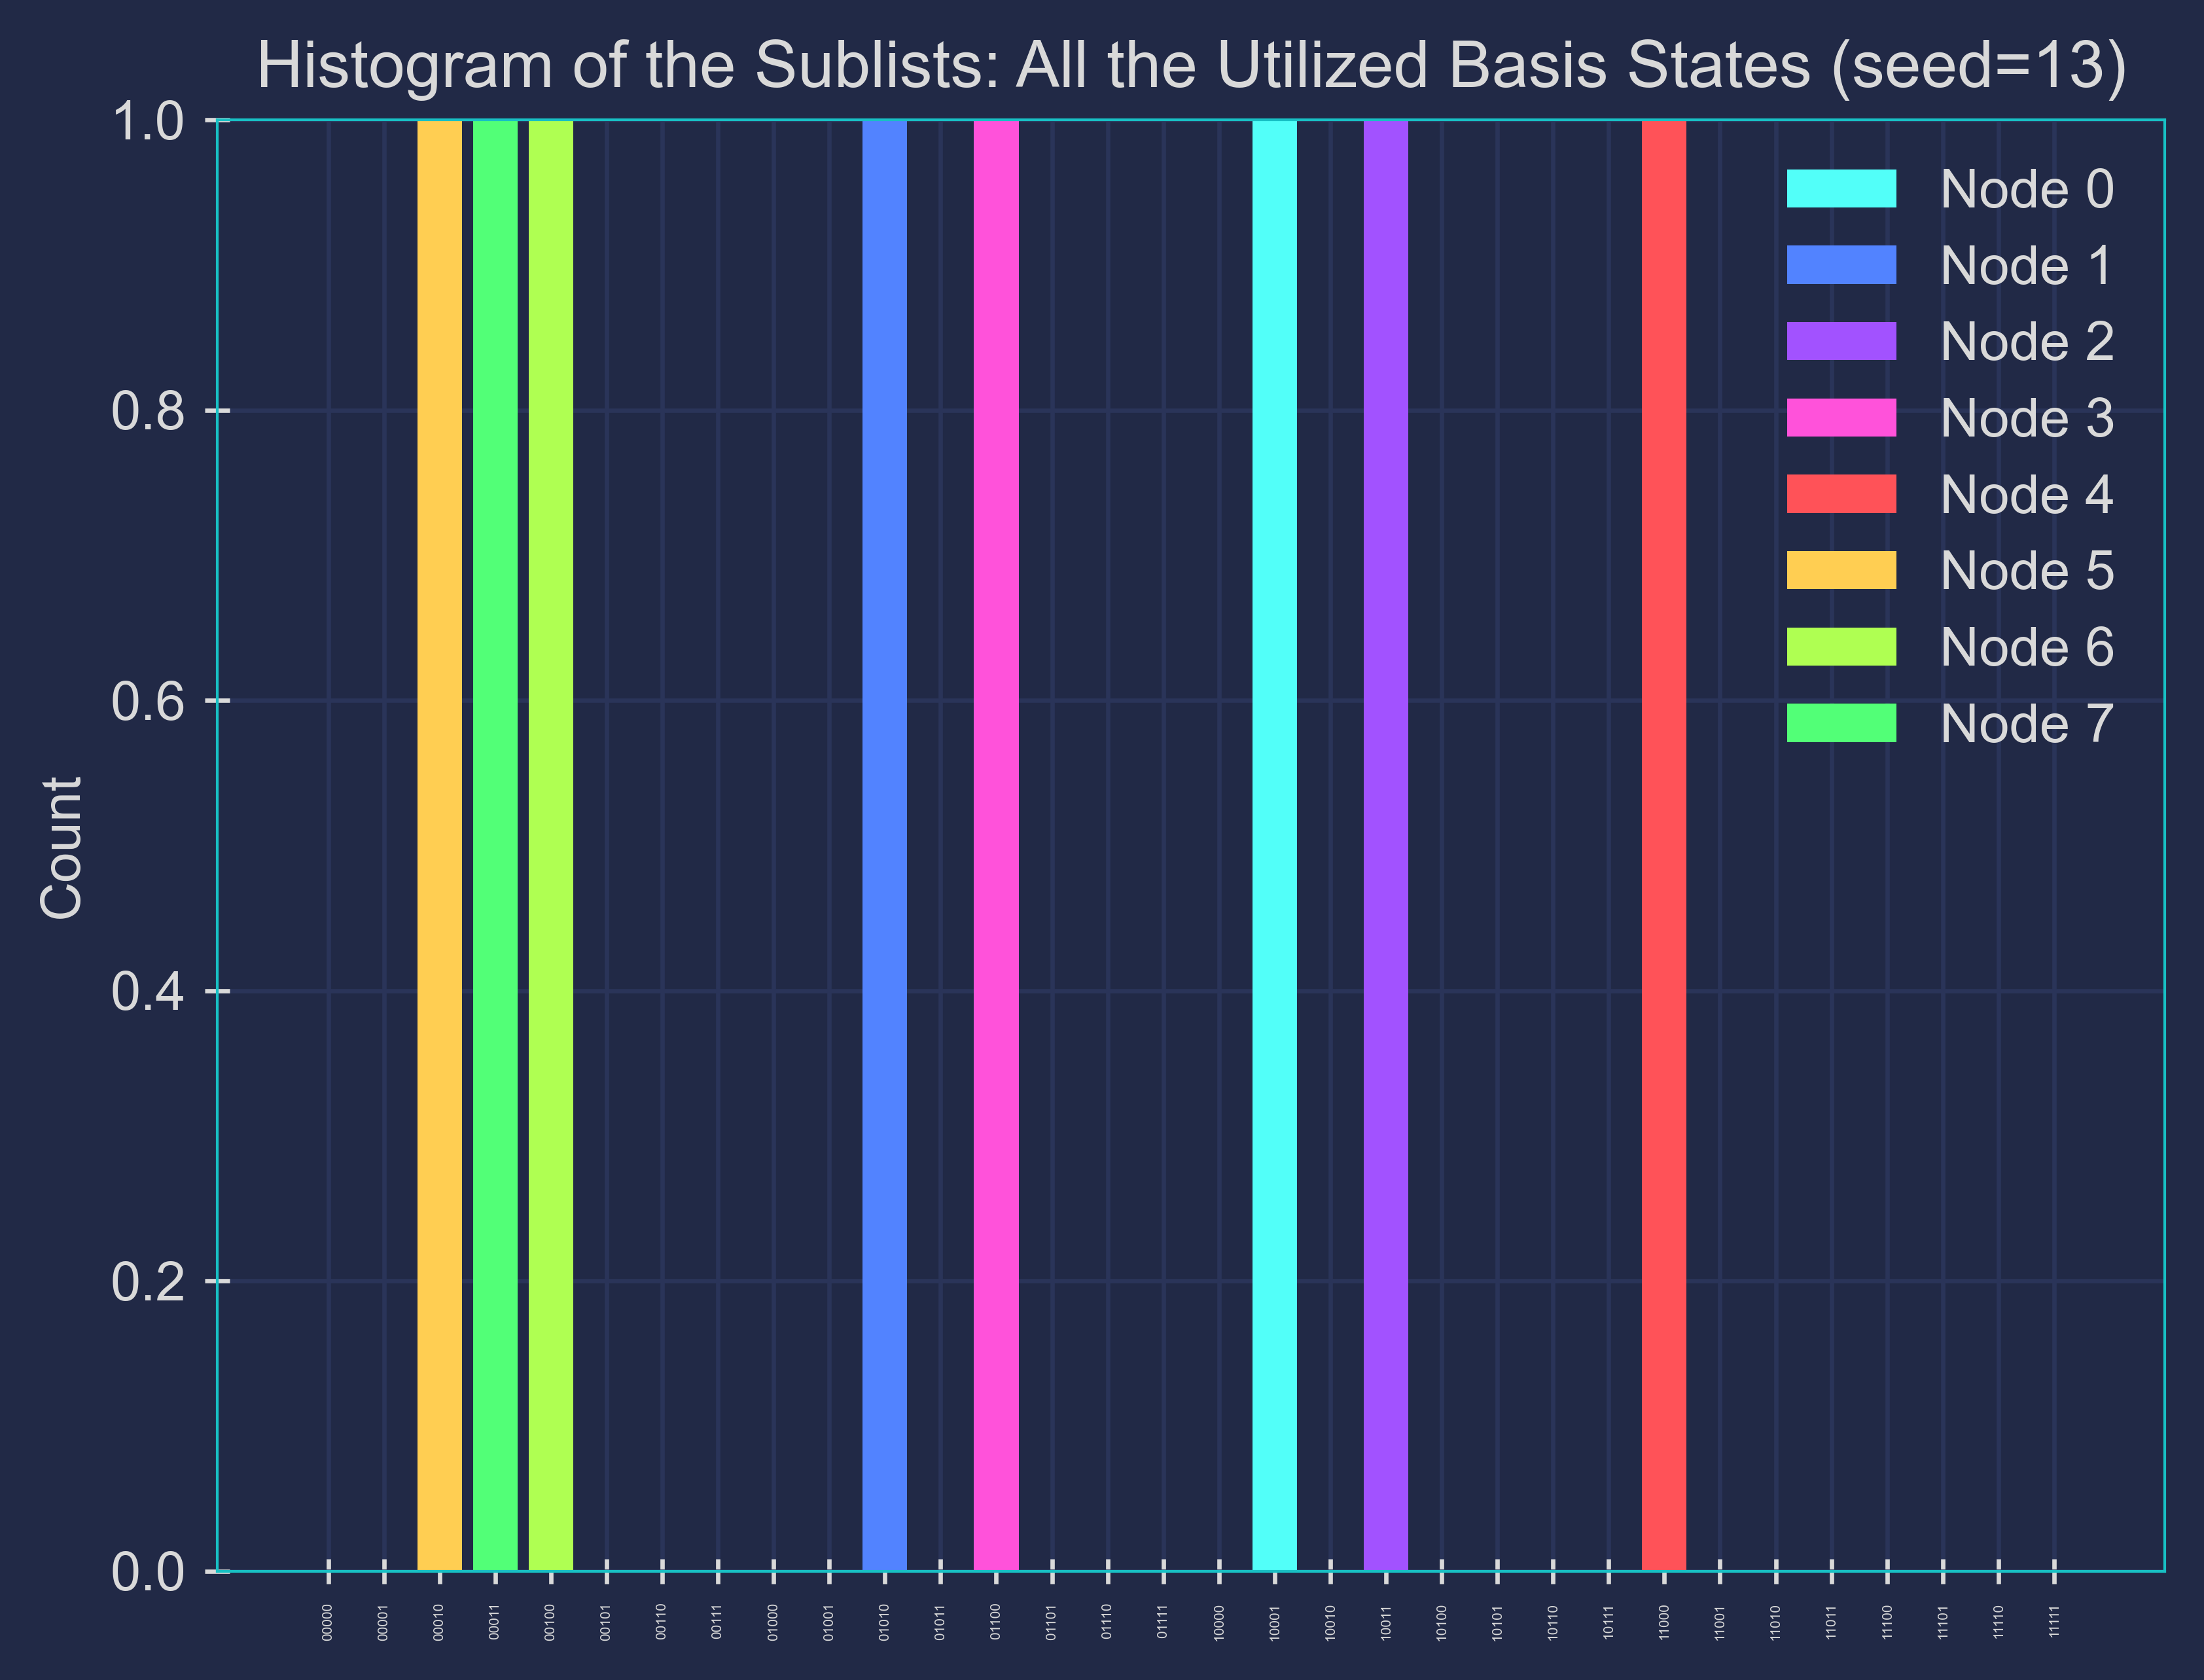
\includegraphics[width=1\textwidth,height=0.75\textwidth]{Figures/Chapter_5/Random iQAQE (Coloured plots)/8-node(seed=13).png}
      \caption{Seed = $13$.}
      \label{fig:seed=13}
  \end{subfigure}
  \hfill
  \begin{subfigure}[t]{0.495\textwidth}
      \centering
      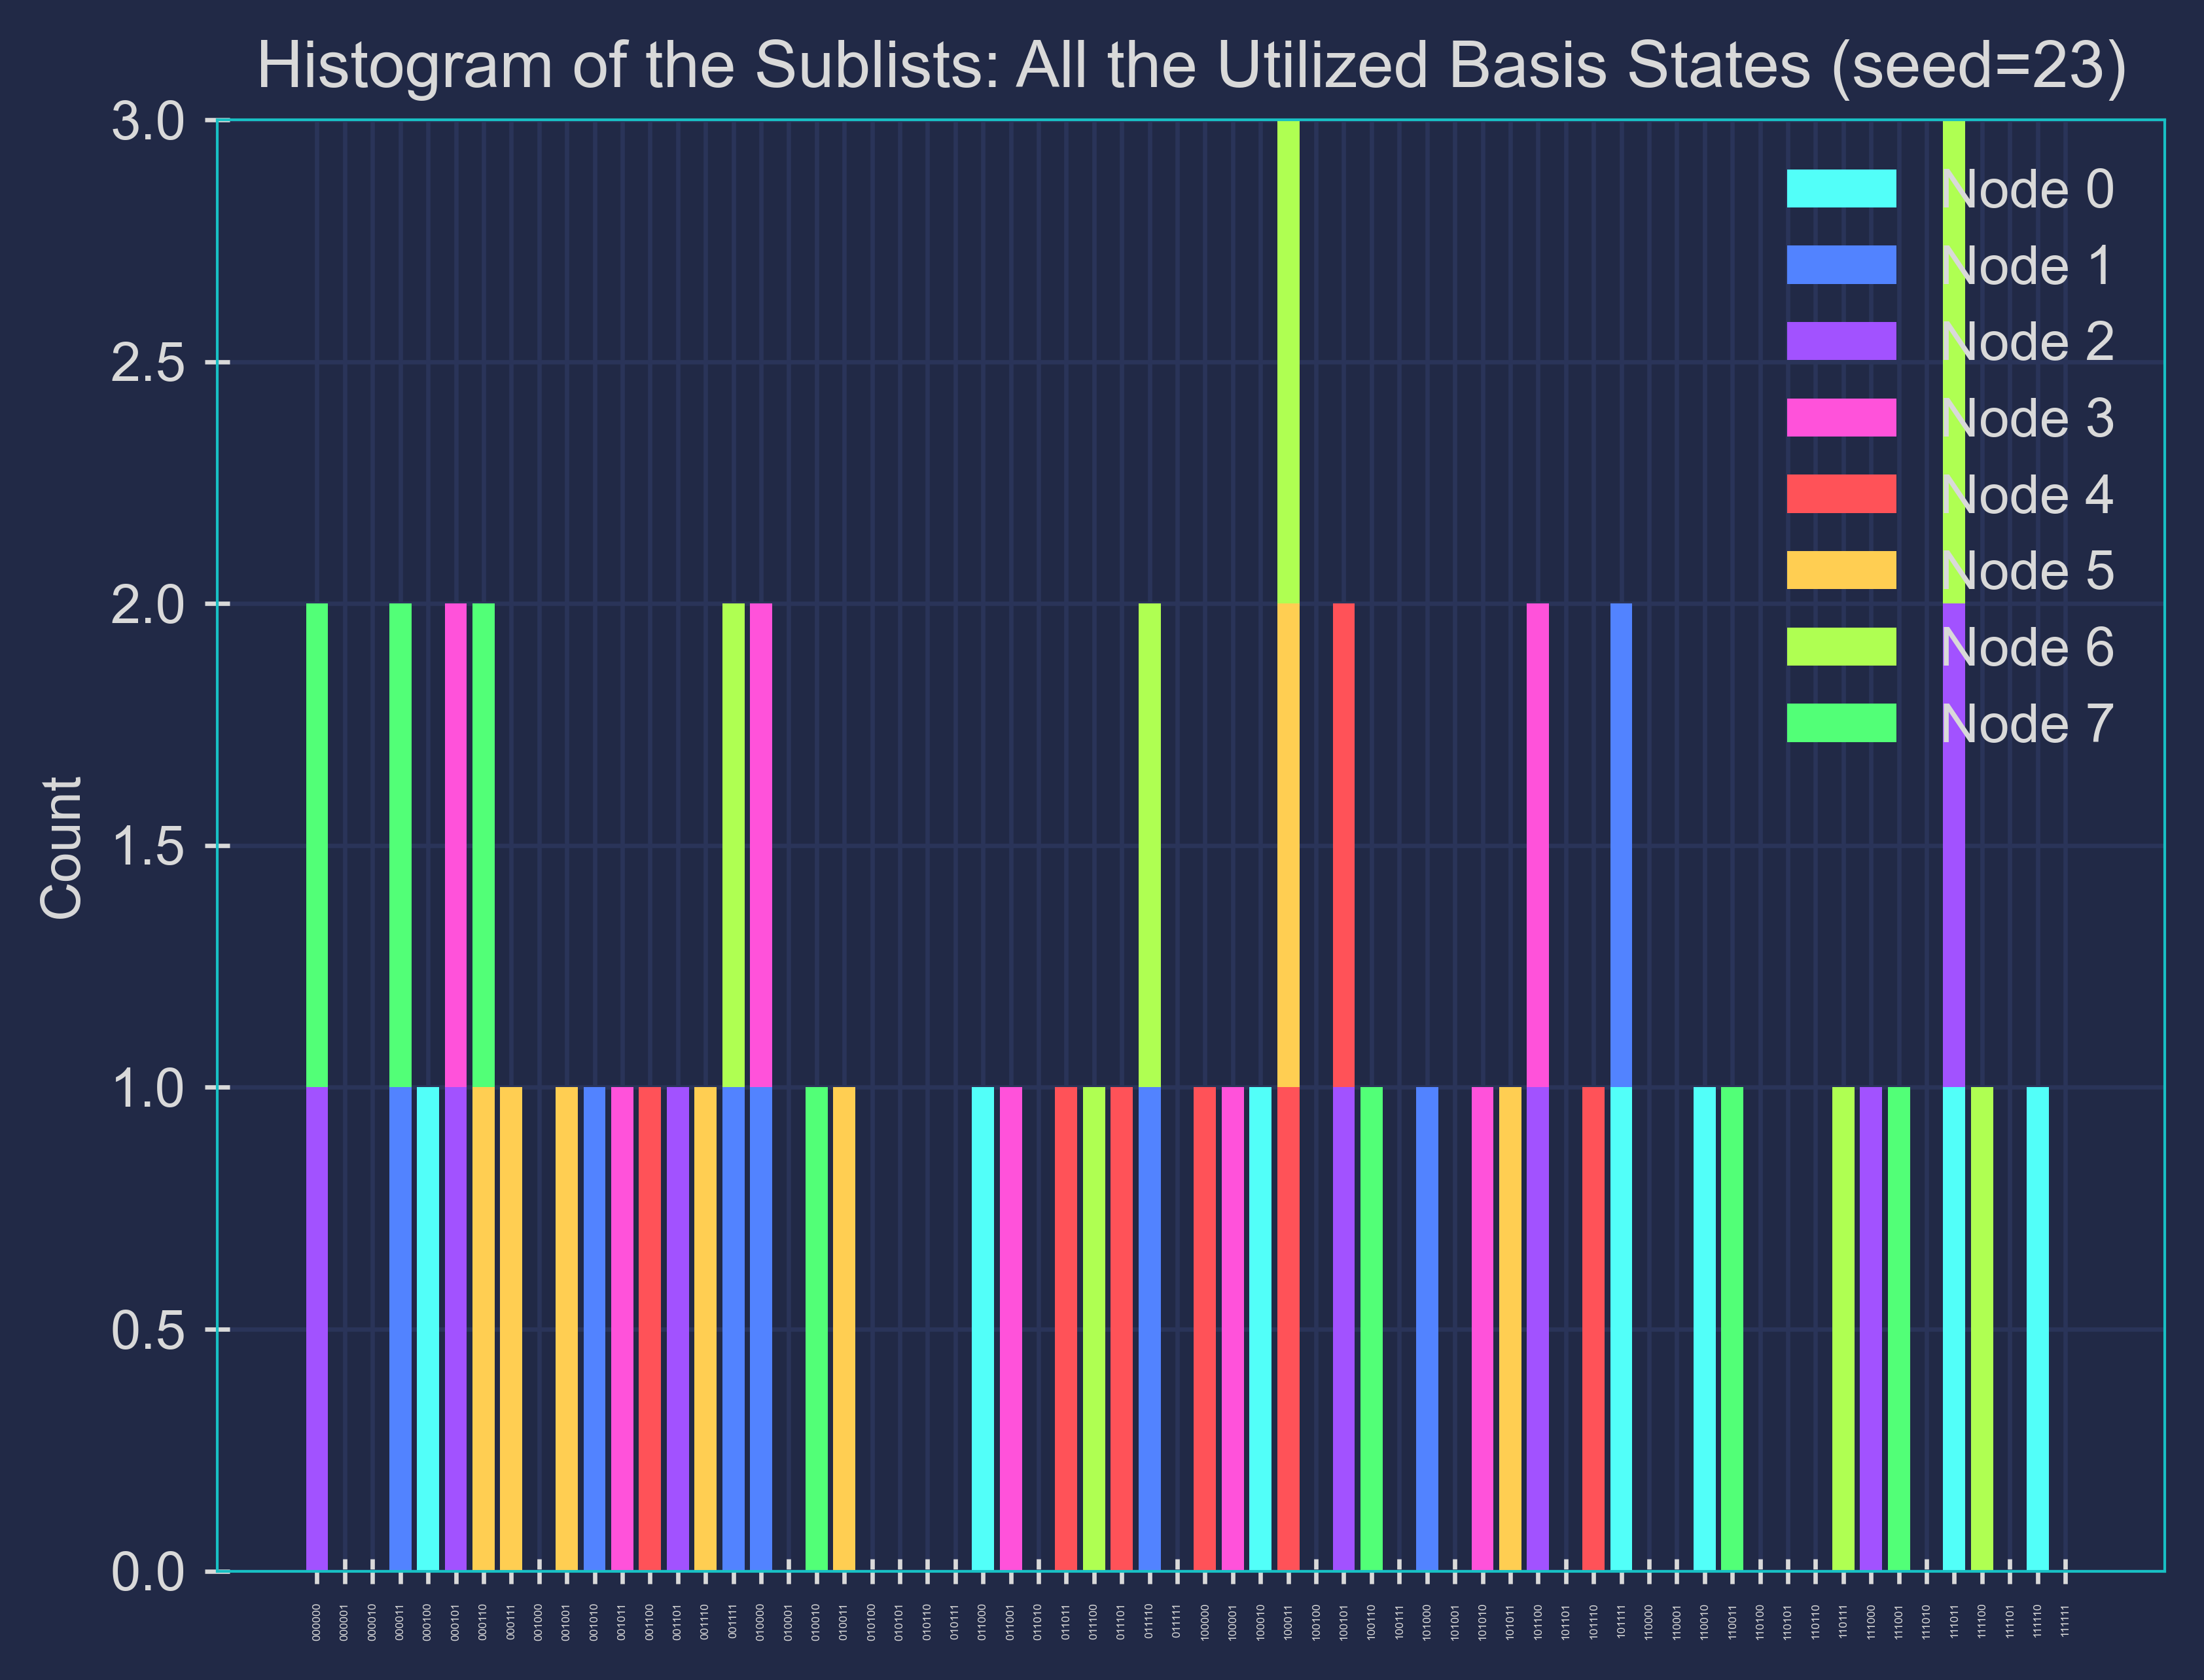
\includegraphics[width=1\textwidth,height=0.75\textwidth]{Figures/Chapter_5/Random iQAQE (Coloured plots)/8-node(seed=23).png}
      \caption{Seed = $23$.}
      \label{fig:seed=23}
  \end{subfigure}
\end{figure*}

% \bigskip

\clearpage

\begin{figure*}[ht!]
  \addtocounter{figure}{-1} % Added <<
  \centering
  \begin{subfigure}[t]{0.325\textwidth}
      \addtocounter{subfigure}{2} % Added <<
      \centering
      \includegraphics[width=1\textwidth,height=4.25cm]{Figures/Chapter_5/Random iQAQE (Coloured plots)/8-node(seed=26).png}
      \caption{Seed = $26$.}
      \label{fig:seed=26}
  \end{subfigure}
  \hfill
  \begin{subfigure}[t]{0.325\textwidth}
      \centering
      \includegraphics[width=1\textwidth,height=4.25cm]{Figures/Chapter_5/Random iQAQE (Coloured plots)/8-node(seed=38).png}
      \caption{Seed = $38$.}
      \label{fig:seed=38}
  \end{subfigure}
  \hfill
  \begin{subfigure}[t]{0.325\textwidth}
      \centering
      \includegraphics[width=1\textwidth,height=4.25cm]{Figures/Chapter_5/Random iQAQE (Coloured plots)/8-node(seed=39).png}
      \caption{Seed = $39$.}
      \label{fig:seed=39}
  \end{subfigure}
  \caption{Basis states' distributions over the $8$ nodes of the usual graph for many different \texttt{np.random.seed} seeds. Only those for which the best-so-far average approximation ratio after $100$ \acrshort{iqaqe} iterations was found to be $\geq 0.975$ were selected. (These were the best performing seeds out of the $50$ tested, for \texttt{seed} $\in \left[0, 49\right] \cap \mathbb{Z}$.)}
  \label{fig:Random_iQAQE(Seeds)}
\end{figure*}

As can be seen, not much can be directly inferred from this. When confronted with seemingly unstructured data, a natural progression is to employ machine learning schemes to discern patterns. Indeed, this aligns with the forte of such models. Various options were considered, spanning from neural networks to regression and clustering models. Initially, we opted to implement a basic regression model for its simplicity. Establishing such a model necessitates identifying a set of statistical properties of the input data (lists of basis states) that can serve as inputs for the regression model. This discussion follows in the subsequent section.

\vspace{-2.5mm}
\subsection*{Machine learning-based approach}
Following the prior discussion regarding the \acrshort{iqaqe} formalism (refer to Figure \ref{fig:Random_iQAQE(Seeds)}), our objective was to construct a small machine learning (\acrshort{ml}) model aimed at comprehending the patterns in basis states' partitioning that contribute to the algorithm's performance variations. Naturally, such a model necessitates defining input (independent variables - \acrshort{iv}\textcolor{gray}{s}) and output (dependent variable - \acrshort{dv}). As previously mentioned, our \acrshort{iv}\textcolor{gray}{s} will encompass statistically significant properties extracted from each specific sub-list. Alternatively, including the basis states' mapping directly as the model's input presents challenges concerning memory-efficient encoding. Traditional one-hot encoding methods are inadequate due to the vast number of potential basis states available (which scales exponentially with the number of qubits). Thus, we opted for the following statistical properties:
\begin{itemize}
  \item {\large\textbf{Type $1$ variables}} - these are input variables that are defined for each of the sub-lists of basis states. They are:
  \begin{itemize}
      \item \textbf{Number of basis states} in each sub-list, the so-called cardinality of the sub-list;
      \item \textbf{Average Hamming weight} in each sub-list;
      \item \textbf{Standard deviation/variance of the Hamming weights} in each sub-list;
      \item \textbf{Average pair-wise Hamming distance} between the basis states in each sub-list;
      \item \textbf{Standard deviation/variance of the pair-wise Hamming distances} between the basis states in each sub-list;
      \item \textbf{Parity score} of each sub-list: this is obtained by: \#(Even basis states) $-$ \#(Odd basis states), for each sub-list.
  \end{itemize}
  \item {\large\textbf{Type $2$ variables}} - these are input variables that are defined for the entire set of basis states. They are:
  \begin{itemize}
      \item \textbf{Average Hamming weight} of the entire set of basis states;
      \item \textbf{Standard deviation/variance of the Hamming weights} of the entire set of basis states;
      \item \textbf{Average pair-wise Hamming distance} between the basis states in the entire set;
      \item \textbf{Standard deviation/variance of the pair-wise Hamming distances} between the basis states in the entire set;
      \item \textbf{Parity score} of the entire set of basis states. (Given by the sum of the parity scores of the sub-lists);
      \item \textbf{Global basis-states' entropy} [of the entire set of basis states]: this is given by the Shannon entropy of the basis states' distribution in the entire set. It is calculated as: $-\frac{1}{\log_2(N)}\sum_{i=1}^{N} p_i \log_2(p_i)$, where $p_i$ is the probability of the $i^{th}$ basis state in the entire set. Note that it is normalized by the maximum entropy value, which is $\log_2(N)$, where $N$ is the total number of basis states in the entire set. (This entropy's maximum is achieved when we have a uniform distribution of the basis states.) Also, this is a measure of the randomness of the basis states' distribution in the entire set.
  \end{itemize}
\end{itemize}
The dataset was constructed in a similar manner to that of Figure \ref{fig:Random_iQAQE(Seeds)}, but expanded to encompass $1000$ seeds. For each seed, we computed the \textbf{median} \acrshort{bsf} cut value after training (\acrshort{dv}) and the associated independent variables (\acrshort{iv}\textcolor{gray}{s}) related to the partitioning of basis states. (It's worth noting that we employed \texttt{n\_layers = 3}, \texttt{step\_size = 0.99}, \texttt{B = 4}, \texttt{max\_iter = 50}, and \texttt{repeat = 5}, i.e., $5$ repetitions for each seed.)

With the \acrshort{iv}\textcolor{gray}{s} and \acrshort{dv} finally chosen, and the data set fully constructed, we now need to define our model. We decided to start simple, with a basic multiple linear regression model. Here, the \acrshort{dv} is computed as a linear combination of the \acrshort{iv}\textcolor{gray}{s}, as below:
\begin{equation}
    y = \beta_0 + \beta_1 x_1 + \beta_2 x_2 + \ldots + \beta_n x_n + \epsilon,
\end{equation}
where $x_i$ are the input variables (\acrshort{iv}\textcolor{gray}{s}), $y$ is the dependent variable (\acrshort{dv}), $\beta_i$ are the coefficients, and $\epsilon$ is the error term. The coefficients will be estimated using the Ordinary Least Squares (OLS) method. The model's goodness-of-fit will be evaluated using the $R^2$ value. Additionally, it's worth noting that the independent variables were scaled using the \texttt{StandardScaler} from the \texttt{sklearn.preprocessing} module, a common practice in machine learning. This process standardizes the features by removing their mean and scaling them to unit variance, ensuring they have equal weight in the model. This standardization provides a stable foundation for both multiple linear regression and Principal Component Analysis (\acrshort{pca}).

% Re-read from here, downwards.
After implementing the model, we obtained an $R^2$ of $0.1023$, which is far from the ideal value of $1$, and a $5$-fold cross-validation loss of $0.0061$ (average mean square error) with a standard deviation of $0.0004$. To improve the model, I analyzed the independent variables (\acrshort{iv}\textcolor{gray}{s}) by examining their correlation matrix and Variance Inflation Factor (\acrshort{vif}). The correlation matrix revealed that some \acrshort{iv}\textcolor{gray}{s} were highly correlated, which was expected in hindsight. High correlation among \acrshort{iv}\textcolor{gray}{s} is problematic because it makes it difficult to isolate the effects of each \acrshort{iv} on the dependent variable (\acrshort{dv}), as altering one \acrshort{iv} affects others.

To quantify this issue, we calculated the \acrshort{vif} for each \acrshort{iv}. The \acrshort{vif} measures the increase in the variance of parameter estimates if an additional variable is added to the linear regression, indicating the level of multicollinearity among the \acrshort{iv}\textcolor{gray}{s}. If the \acrshort{vif} is greater than $5$ or $10$ (depending on the user's tolerance), it suggests high multicollinearity, and the variable should probably be removed from the model. Our analysis showed that many input variables were perfectly multicollinear, meaning some were essentially redundant. I experimented with removing these redundant variables one by one to improve model performance. While this approach did lead to some improvement, it was never significant. I tried various combinations, such as removing only Type $2$ variables, only Type $1$ variables, or a mix of both, but none resulted in substantial performance enhancements. The predictive power of the model was also unsatisfactory. Although it could estimate the order of magnitude correctly, it was often off by more than $0.1$ in approximation ratio (\acrshort{ar}), which is unacceptable. If we could develop a model that accurately predicts the (\acrshort{ar}) based on certain \acrshort{iv}\textcolor{gray}{s}, we could reverse-engineer the sub-lists that lead to the best-performing median \acrshort{bsf} approximation ratios. This would be a significant step towards our ultimate goal of identifying effective partitioning schemes for the basis states.

% Re-write from here on-wards.
In any case, this poor performance could indicate two things: either the model is inadequate (i.e., the underlying relationship is not actually linear), or the chosen \acrshort{iv}\textcolor{gray}{s} are not the most suitable (or, we simply do not have enough data-points; we were limited by the available hardware, so we cannot do much more regarding this). We suspect the latter might be true, although we're unsure which other variables to use. This circles back to the initial challenge of encoding the sub-lists' information in a memory-efficient and representative manner. Regarding the potential non-linearity of the model, we've considered using non-linear models, such as Support Vector Machine Regression (SVR), which exploits the kernel trick to fit non-linear data. However, we have set this idea aside for now\footnote{This would be an interesting direction for future work.}, as our current goal is to identify which \acrshort{iv}\textcolor{gray}{s} most influence the \acrshort{dv}'s value.

One alternative approach that came to mind is to perform Principal Component Analysis (\acrshort{pca}) followed by regression (Principal Component Regression – \acrshort{pcr}). While \acrshort{pca} assumes a linear relationship, it could help us achieve a better model. By computing the Principal Components (\acrshort{pc}\textcolor{gray}{s}), we can indirectly understand which \acrshort{iv}\textcolor{gray}{s} have the greatest influence in explaining the variance of the input data. These influential \acrshort{iv}\textcolor{gray}{s} would be the ones we should focus on when choosing our basis states' partitioning. By examining the loadings of the \acrshort{pc}\textcolor{gray}{s}, we can determine which \acrshort{iv}\textcolor{gray}{s} constitute each \acrshort{pc}. Another advantage of \acrshort{pca} is that the obtained \acrshort{pc}\textcolor{gray}{s} are orthogonal (uncorrelated), thus eliminating the multicollinearity problem among the input variables. We can then attempt linear fitting on the \acrshort{pc}\textcolor{gray}{s} against the \acrshort{dv} (\acrshort{pcr}). The main drawback is that we lose some interpretability of the input variables, as accurately interpreting the \acrshort{pc}\textcolor{gray}{s} can be challenging due to their nature as linear combinations of the original \acrshort{iv}\textcolor{gray}{s}.

Anyways, \acrshort{pcr} using the $5$ most significant principal components also yielded subpar results. An $R^2$ of $0.0287$ was reported, with a $5$-fold cross-validation loss of $0.0059$ and a standard deviation of $0.0004$. As one could already predict from the $R^2$ value, this model's predictive powers were also unsatisfactory. Nevertheless, we can still try to extract some information from the principal components to understand which independent variables are most influential in determining the dependent variable. Notably, the first $5$ principal components (out of $47$) account for $65.3\%$ of the variance in the data:
\begin{lstlisting}[caption={Explained variance ratio for the first $5$ \acrshort{pc}\textcolor{gray}{s} ($8$-node graph).}, captionpos=b, style=DOS]
  Explained variance ratio:
  [0.46558461 0.07637042 0.04557191 0.03879498 0.02634421]
\end{lstlisting}
Now, if we examine the loadings of the first and most significant principal component, we notice they are quite evenly distributed across the independent variables. This makes interpretation challenging, as we cannot easily identify one \acrshort{iv} as being more important than the others. Here are the loadings of the first principal component for the $8$-node graph: (Identically uniform distributions were also verified for the other \acrshort{pc}\textcolor{gray}{s}.)
\begin{lstlisting}[caption={Loadings of the first \acrshort{pc}, for the $8$-node graph.}, captionpos=b, style=DOS]
  PCA_1 = [-1.75323157e-01 -9.26451207e-02 -8.98377538e-02 -8.77605361e-02 -9.18316965e-02
           -8.58000439e-02 -1.03221966e-01 -9.24948614e-02 -1.11659776e-01 -1.75791034e-01
           -1.73978061e-01 -1.70204027e-01 -1.70707746e-01 -1.73770114e-01 -1.72400120e-01
           -1.73386482e-01 -1.71136657e-01 -1.88767128e-01 -1.82462202e-01 -1.81233077e-01
           -1.81277591e-01 -1.83509589e-01 -1.80911686e-01 -1.83449672e-01 -1.85536765e-01
           -1.87937749e-01 -1.85009049e-01 -1.87993729e-01 -1.86774034e-01 -1.87581036e-01
           -1.85531361e-01 -1.86124394e-01 -1.86528612e-01 -2.09742228e-03 -3.66652955e-03
            9.18121507e-04 -9.31248048e-03 -4.63173882e-03 -1.18673071e-03  1.43514268e-02
           -1.14790537e-02 -1.48687943e-01 -1.33654722e-01 -1.54547996e-01 -1.55191025e-01
           -5.69361380e-03 -1.50033651e-01]
  \end{lstlisting}
As can be seen, there are no \acrshort{iv}\textcolor{gray}{s} whose impact can be neglected, making the interpretation of this principal component nearly impossible, which doesn't help our case much. Ideally, we would discover that a small number of independent variables have a significantly larger impact than the others. This would enable us to concentrate on those variables when selecting our basis states' partitioning. Unfortunately, this is not the situation here. For the sake of completeness and organization, I compile the obtained results in the following table (Table \ref{tab:Scaled_Median_BSF_Table_8-node}).
\begin{table}[H]
  \centering
  \begin{tabular}{|c|cc|c|}
  \hline
  \rowcolor[HTML]{FFFFFF} 
  \cellcolor[HTML]{FFFFFF}                               & \multicolumn{2}{c|}{\cellcolor[HTML]{FFFFFF}$5$-fold cross-validation loss} & \cellcolor[HTML]{FFFFFF} \\ \cline{2-3}
  \rowcolor[HTML]{FFFFFF} 
  \multirow{-2}{*}{\cellcolor[HTML]{FFFFFF}Model ($8$-node graph)} &
    \multicolumn{1}{c|}{\cellcolor[HTML]{FFFFFF}Average ($\overline{x}$)} &
    Std. dev. ($\sigma$) &
    \multirow{-2}{*}{\cellcolor[HTML]{FFFFFF}$R^2$} \\ \hline
  \rowcolor[HTML]{EFEFEF} 
  \cellcolor[HTML]{FFFFFF}Multiple Linear Regression     & \multicolumn{1}{c|}{\cellcolor[HTML]{EFEFEF}0.0061}         & 0.0004        & 0.1023                   \\ \hline
  \rowcolor[HTML]{EFEFEF} 
  \cellcolor[HTML]{FFFFFF}\acrshort{pcr} ($5$ Principal Components) & \multicolumn{1}{c|}{\cellcolor[HTML]{EFEFEF}0.0059}         & 0.0004        & 0.0287                   \\ \hline
  \end{tabular}
  \caption{Cross-validation loss (average mean square error) and $R^2$ values for the two fitted models, Multiple Linear Regression and \acrshort{pcr}, in the context of the usual $8$-node graph.}
  \label{tab:Scaled_Median_BSF_Table_8-node}
\end{table}

% Re-read this part! Last thing for today (18/05/2024)! " – in absolute value" I removed this!
Furthermore, after revisiting the regression analyses' coefficients, we noticed something curious: when not performing \acrshort{pca} before fitting\footnote{If PCA is applied before fitting (\acrshort{pcr}), the linear regression coefficients remain stable within the range \([10^{-4}, 10^{-3}]\) in absolute value and do not diverge.}, we observed significantly higher coefficients for four specific input variables (on the order of magnitude \(10^9\) or \(10^{10}\), compared to \([10^{-4}, 10^{-2}]\) for all other variables). These \acrshort{iv}\textcolor{gray}{s} are (for the $8$-node graph dataset):
\begin{enumerate}
    \item Average Hamming weight (Type $1$);
    \item Parity Score (Type $1$);
    \item Average Hamming weight (Type $2$);
    \item Parity Score (Type $2$).
\end{enumerate}
Initially, it appeared that these variables contributed the most to the dependent variable's value (median best-so-far approximation ratio after training). However, we no longer believe that to be the case. Instead, we attribute this observation to high multicollinearity among the independent variables (\acrshort{iv}\textcolor{gray}{s}), which renders the model unstable.

We also tested Ridge regression ($L2$ regularization) as an alternative to \acrshort{pcr}. Ridge regression is useful when the input data has obvious multicollinearity, as it adds a penalty to the regression coefficients, reducing their variance and stabilizing the model. Using \texttt{alpha = 1.0} in \texttt{sklearn.linear\_model.Ridge}, we obtained an \(R^2\) value of $0.1023$ and an average cross-validation loss of $0.0061$, with a standard deviation of $0.0004$. These results were identical to those from multiple linear regression (for the $8$-node graph). However, with Ridge regression, no \acrshort{iv}\textcolor{gray}{s} had disproportionately large coefficients; they all ranged between \(10^{-4}\) and \(10^{-2}\). This regularization added stability to the model by preventing coefficient divergence. Moreover, its predictive power appeared to be slightly better than that of regular linear regression for our current dataset, often resulting in errors smaller than $0.1$ in approximation ratio (\acrshort{ar}).

This analysis reinforced our belief that the previous \(10^{10}\)-valued coefficients were due to model instabilities from high multicollinearity. Thus, Ridge regression offers a better model with more meaningful and interpretable coefficients. However, the uniform spread of coefficients makes it difficult to pinpoint a few \acrshort{iv}\textcolor{gray}{s} as the most impactful, which we had hoped to identify.

We have explored several techniques to find patterns or strategies for better mapping. However, the task is more complex than initially anticipated. Capturing all intricate patterns might require a more complex model, such as a neural network or another non-linear approach. We have decided to leave this direction for future work. Another concern is that \acrshort{iqaqe}'s performance may depend heavily on the specific graph instance, complicating the generalization of a model for predicting optimal mapping strategies. Despite this, we believe it is still worth pursuing.

% I don't actually include here the last analysis that we performed: scores histogram. To assess their performance. For $1000$ seeds. Should I include this? I don't think it is absolutely necessary, but w/e.

% Ridge regression? Is there anything else I should add here, from the logbook? Maybe, re-read both this and the logbook, to see if there's anything I should add here.

% Actually, I think I should just include the 'scaled' results. Re-read this and change some things: like, e.g., in the 'scaled' version, we use the median best-so-far!

% Mention multi-collinearities, VIF;
% Introduce PCA as a means to combat that. This took our analysis in a different direction, as we began to explore the use of PCA to reduce the multi-collinearity, and extract the most important features. (No need to present all the results that I've obtained, though.)

% Explain that the idea is that we should be able to re-construct the sub-lists, from good-performing IVs. This is the ultimate goal of this analysis.

% Still, I think we should include the PCA results showing that there doesn't appear to be 'one' more important PC. This gives us some lights: probably, the intricate patterns that we're hoping to find are much more graph dependent than we initially thought. This is a good insight, and it's worth mentioning. Although, it definitely makes our job of finding good partitioning schemes much harder.

% % ----------------------------------------------------------------------
% \subsection{Figures}
% \label{subsection:figures}

% Insert your section material and possibly a few figures.

% Make sure all figures presented are referenced in the text!

% The caption should appear below the figure.


% % ----------------------------------------------------------------------
% \subsubsection{Images}
% \label{subsection:images}

% By default, this document supports file types {\it .png,.pdf,.jpg,,.jpeg}.

% See the documentation of package {\it graphicx} \url{https://www.ctan.org/tex-archive/macros/latex/required/graphics/} for other extensions support.

% When referencing a figure, use the abbreviation Fig., unless it is the beginning of a sentence.

% Figure~\ref{fig:airbus1} is an example and so is Fig.~\ref{fig:aircraft}.

% \begin{figure}[!htb]
%   \centering
%   \includegraphics[width=0.25\textwidth]{Figures/Airbus_A350.jpg}
%   \caption[Optional caption for figure in TOC.]{Caption for figure.}
%   \label{fig:airbus1}
% \end{figure}

% It is possible to include subfigures.
% Figure~\ref{fig:aircraft} is composed of three subfigures: Fig.~\ref{fig:aircraft1}, \ref{fig:aircraft2} and \ref{fig:aircraft3}.
% %
% \begin{figure}[!htbp]
%     \centering
%     \subfloat[Airbus A320.\label{fig:aircraft1}]{\includegraphics[width=0.49\textwidth]{Figures/Airbus_A320_sharklets.png}]{fig1a}}\hfill
%     \subfloat[Bombardier CRJ200.\label{fig:aircraft2}] {\includegraphics[width=0.49\linewidth]{Figures/Bombardier_CRJ200.png}}\hfill
%     \subfloat[Airbus A350.\label{fig:aircraft3}]{\includegraphics[width=0.49\textwidth]{Figures/Airbus_A350.jpg}}
%     \caption{Examples of aircraft.} \label{fig:aircraft}
% \end{figure}

% Most aircraft have wings with large aspect ratios (\AR = 8 -- 15) for higher aerodynamic efficiency.


% % ----------------------------------------------------------------------
% \subsubsection{Drawings}
% \label{subsection:drawings}

% Insert your subsection material and for instance a few drawings.

% The schematic illustrated in Fig.~\ref{fig:algorithm} can represent some sort of algorithm.

% \begin{figure}[!htb]
%   \centering
%   \scriptsize
% %  \footnotesize 
% %  \small
%   \setlength{\unitlength}{0.9cm}
%   \begin{picture}(8.5,6)
%     \linethickness{0.3mm}

%     \put(3,6){\vector(0,-1){1}}
%     \put(3.5,5.4){$\bf \alpha$}
%     \put(3,4.5){\oval(6,1){}}
%     %\put(0,4){\framebox(6,1){}}
%     \put(0.3,4.4){Grid Generation: \quad ${\bf x} = {\bf x}\left({\bf \alpha}\right)$}

%     \put(3,4){\vector(0,-1){1}}
%     \put(3.5,3.4){$\bf x$}
%     \put(3,2.5){\oval(6,1){}}
%     %\put(0,2){\framebox(6,1){}}
%     \put(0.3,2.4){Flow Solver: \quad ${\cal R}\left({\bf x},{\bf q}\left({\bf x}\right)\right) = 0$}

%     \put(6.0,2.5){\vector(1,0){1}}
%     \put(6.4,3){$Y_1$}

%     \put(3,2){\vector(0,-1){1}}
%     \put(3.5,1.4){$\bf q$}
%     \put(3,0.5){\oval(6,1){}}
%     %\put(0,0){\framebox(6,1){}}
%     \put(0.3,0.4){Structural Solver: \quad ${\cal M}\left({\bf x},{\bf q}\left({\bf x}\right)\right) = 0$}

%     \put(6.0,0.5){\vector(1,0){1}}
%     \put(6.4,1){$Y_2$}

%     %\put(7.8,2.5){\oval(1.6,5){}}
%     \put(7.0,0){\framebox(1.6,5){}}
%     \put(7.1,2.5){Optimizer}
%     \put(7.8,5){\line(0,1){1}}
%     \put(7.8,6){\line(-1,0){4.8}}
%   \end{picture}
%   \caption{Schematic of some algorithm.}
%   \label{fig:algorithm}
% \end{figure}


% % ----------------------------------------------------------------------
% \subsection{Equations}
% \label{subsection:equations}

% Equations can be inserted in different ways.

% The simplest way is in a separate line as

% \begin{equation}
%   \frac{{\rm d} q_{ijk}}{{\rm d} t} + {\cal R}_{ijk}({\bm q}) = 0 \,,
% \label{eq:ode}
% \end{equation}
% %
% where each variable must properly defined.

% If the equation is to be embedded in the text, it can be done like ${\partial {\cal R}}/{\partial {\bm q}}=0$.

% It may also be split in different lines like

% \begin{eqnarray}
%   {\rm Minimize}   && Y({\bm \alpha},{\bm q}({\bm \alpha}))            \nonumber           \\
%   {\rm with~respect~to}     && {\bm \alpha}                                     \label{eq:minimize} \\
%   {\rm subject~to} && {\cal R}({\bm \alpha},{\bm q}({\bm \alpha})) = 0 \nonumber           \\
%                    &&       C ({\bm \alpha},{\bm q}({\bm \alpha})) = 0 \,. \nonumber
% \end{eqnarray}

% It is also possible to use subequations.

% \begin{subequations}
%     \begin{equation}
%     \frac{\partial \rho}{\partial t} + \frac{\partial}{\partial x_j}\left( \rho u_j \right) = 0 \,,
%     \label{eq:continuity}
%     \end{equation}
%     \begin{equation}
%     \frac{\partial}{\partial t}\left( \rho u_i \right) + \frac{\partial}{\partial x_j} \left( \rho u_i u_j + p \delta_{ij} - \tau_{ji} \right) = 0, \quad i=1,2,3 \,,
%     \label{eq:momentum}
%     \end{equation}
%     \begin{equation}
%         \frac{\partial}{\partial t}\left( \rho E \right) + \frac{\partial}{\partial x_j} \left( \rho E u_j + p u_j - u_i \tau_{ij} + q_j \right) = 0 \,.
%     \label{eq:energy}
%     \end{equation}
% \label{eq:NavierStokes}%
% \end{subequations}

% Notice that the equations should be punctuated as they are part of sentences, so a comma or a period should be put at the end of each of them, as exemplified in all the previous equations.

% When referencing an equation, use the abbreviation Eq., unless it is the beginning of a sentence.
% The number of the equation should always be in parenthesis.

% Equations~(\ref{eq:continuity}), (\ref{eq:momentum}) and (\ref{eq:energy}) form the Navier--Stokes equations~(Eq.~ (\ref{eq:NavierStokes})).


% % ----------------------------------------------------------------------
% \subsection{Tables}
% \label{section:tables}

% Insert your subsection material and for instance a few tables.

% Make sure all tables presented are referenced in the text!

% The caption should appear above the table.

% Follow some guidelines when making tables:

% \begin{itemize}
%   \item Avoid vertical lines;
%   \item Avoid “boxing up” cells, usually 3 horizontal lines are enough: above, below, and after heading;
%   \item Avoid double horizontal lines;
%   \item Add enough space between rows.
% \end{itemize}

% \begin{table}[!htb]
%   \caption[Table caption shown in TOC.]{Table caption.}
%   \label{tab:aeroCoeff}
%   \renewcommand{\arraystretch}{1.2} % more space between rows
%   \centering
%   \begin{tabular}{lccc}
%     \toprule
%     Model           & $C_L$ & $C_D$ & $C_{M y}$ \\
%     \midrule
%     Euler           & 0.083 & 0.021 & -0.110    \\
%     Navier--Stokes  & 0.078 & 0.023 & -0.101    \\
%     \bottomrule
%   \end{tabular}
% \end{table}

% When referencing a table, use the abbreviation Tab., unless it is the beginning of a sentence.

% Tables~\ref{tab:memory} and \ref{tab:multipleColumns} are examples of tables with merging columns:

% \begin{table}[!htb]
%   \caption{Memory usage comparison (in MB).}
%   \label{tab:memory}
%   \renewcommand{\arraystretch}{1.2} % more space between rows
%   \centering
%   \begin{tabular}[]{lrr}
%     \toprule
%                 & \multicolumn{2}{c}{\underline{Virtual memory [MB]}} \\
%                 & Euler       & Navier--Stokes \\
%     \midrule
%       Wing only &  1,000      &    2,000       \\
%       Aircraft  &  5,000      &   10,000       \\
%       (ratio)   & $5.0\times$ & $5.0\times$    \\
%     \bottomrule
%   \end{tabular}
% \end{table}

% \begin{table}[!htb]
%   \caption{Another table caption.}
%   \label{tab:multipleColumns}
%   \centering
%   \renewcommand{\arraystretch}{1.2} % more space between rows
%   \begin{tabular}{@{}rrrrcrrr@{}} % remove space to the vertical edges @{}...@{}
%     \toprule
%       & \multicolumn{3}{c}{$w = 2$} & \phantom{abc} & \multicolumn{3}{c}{$w = 4$} \\
%     \cmidrule{2-4}
%     \cmidrule{6-8}
%       & $t=0$ & $t=1$ & $t=2$ && $t=0$ & $t=1$ & $t=2$ \\
%     \midrule
%       $dir=1$
%       \\
%       $c$ &  0.07 &  0.16 &  0.29 &&  0.36 &  0.71 &   3.18 \\
%       $c$ & -0.86 & 50.04 &  5.93 && -9.07 & 29.09 &  46.21 \\
%       $c$ & 14.27 &-50.96 &-14.27 && 12.22 &-63.54 &-381.09 \\
%       $dir=0$
%       \\
%       $c$ &  0.03 &  1.24 &  0.21 &&  0.35 & -0.27 &  2.14 \\
%       $c$ &-17.90 &-37.11 &  8.85 &&-30.73 & -9.59 & -3.00 \\
%       $c$ &105.55 & 23.11 &-94.73 &&100.24 & 41.27 &-25.73 \\
%     \bottomrule
%   \end{tabular}
% \end{table}

% An example with merging rows can be seen in Tab.~\ref{tab:multipleRows}.

% \begin{table}[!htb]
%   \caption{Yet another table caption.}
%   \label{tab:multipleRows}
%   \renewcommand{\arraystretch}{1.2} % more space between rows
%   \centering
%   \begin{tabular}{ccccc}
%     \toprule
%       \multirow{2}{*}{ABC} & \multicolumn{4}{c}{header} \\
%       \cmidrule{2-5} & 1.1 & 2.2 & 3.3 & 4.4 \\
%     \midrule
%       \multirow{2}{*}{IJK} & \multicolumn{2}{c}{\multirow{2}{*}{group}} & 0.5 & 0.6 \\
%       \cmidrule{4-5}       & \multicolumn{2}{c}{}                       & 0.7 & 1.2 \\
%     \bottomrule
%   \end{tabular}
% \end{table}

% If a table has too many columns, it can be scaled to fit the text width, as in Tab.~\ref{tab:scale}.
% %
% \begin{table}[!htb]
%   \caption{Very wide table.}
%   \label{tab:scale}%
%   \renewcommand{\arraystretch}{1.2} % more space between rows
%   \centering
%   \resizebox*{\textwidth}{!}{%
%     \begin{tabular}[]{lcccccccccc}
%       \toprule
%         Variable &  a  &  b  &  c  &  d  &  e  &  f  &  g  &  h  &  i  &  j  \\
%       \midrule
%         Test 1   &  10,000 &  20,000 &  30,000 &  40,000 &  50,000 &  60,000 &  70,000 &  80,000 &  90,000 & 100,000 \\
%         Test 2   &  20,000 &  40,000 &  60,000 &  80,000 & 100,000 & 120,000 & 140,000 & 160,000 & 180,000 & 200,000 \\
%       \bottomrule
%     \end{tabular}
%   }%
% \end{table}


% % ----------------------------------------------------------------------
% \subsection{Mixing}
% \label{section:mixing}

% If necessary, a figure and a table can be put side-by-side as in Fig.~\ref{fig:side_by_side}

% \begin{figure}[!htb]
%   \begin{minipage}[b]{0.60\linewidth}
%     \centering
%     \includegraphics[width=\linewidth]{Figures/Bombardier_CRJ200}
%   \end{minipage}%
%   \begin{minipage}[b]{0.30\linewidth}
%     \centering
%     \begin{tabular}[b]{lll}
%       \toprule
%         \multicolumn{3}{c}{Legend} \\
%       \midrule
%         A & B & C \\
%         0 & 0 & 0 \\
%         0 & 1 & 0 \\
%         1 & 0 & 0 \\
%         1 & 1 & 1 \\
%       \bottomrule
%     \end{tabular}
%     \vspace{5em}
%   \end{minipage}
% \caption{Figure and table side-by-side.}
% \label{fig:side_by_side}
% \end{figure}

 % file "Thesis_Results.tex"
\cleardoublepage

%%%%%%%%%%%%%%%%%%%%%%%%%%%%%%%%%%%%%%%%%%%%%%%%%%%%%%%%%%%%%%%%%%%%%%%%
%                                                                      %
%     File: Thesis_Conclusions.tex                                     %
%     Tex Master: Thesis.tex                                           %
%                                                                      %
%     Author: Andre C. Marta                                           %
%     Last modified :  4 Mar 2024                                      %
%                                                                      %
%%%%%%%%%%%%%%%%%%%%%%%%%%%%%%%%%%%%%%%%%%%%%%%%%%%%%%%%%%%%%%%%%%%%%%%%

\chapter{Conclusions}
\label{chapter:conclusions}

Insert your chapter material here.


% ----------------------------------------------------------------------
\section{Main Findings}
\label{section:findings}

The major achievements of the present work.


% ----------------------------------------------------------------------
\section{Future Work}
\label{section:future}

A few ideas for future work.

% Just CTRL+F "Future Work" in the main document to find whenever I mention it.

 % file "Thesis_Conclusions.tex"
\cleardoublepage

% ----------------------------------------------------------------------
%  Bibliography
% ----------------------------------------------------------------------

% Add entry in the table of contents as chapter
\phantomsection
\addcontentsline{toc}{chapter}{\bibname}

% Include all references in .bib file, even non-cited ones...
%\nocite{*} % this should be used carefully because it is not correct!

% Produces the bibliography section when processed by BibTeX
%
% Bibliography style
% > entries ordered alphabetically
%\bibliographystyle{plain}
% > unsorted with entries appearing in the order in which the citations appear.
%\bibliographystyle{unsrt}
% > entries ordered alphabetically, with first names and names of journals and months abbreviated
%\bibliographystyle{abbrv}
% > entries ordered alphabetically, with reference markers based on authors' initials and publication year
%\bibliographystyle{alpha}
%
% Replacement bibliography styles provided by 'natbib' package
% (plainnat.bst, abbrvnat.bst, unsrtnat.bst )
% > entries ordered alphabetically
%\bibliographystyle{plainnat}
% > unsorted with entries appearing in the order in which the citations appear.
%\bibliographystyle{unsrtnat}
% > entries ordered alphabetically, with first names and names of journals and months abbreviated
%\bibliographystyle{abbrvnat} % <<<<< SELECT IF USING REFERENCES BY AUTHOR/YEAR
% > entries ordered alphabetically, with reference markers based on authors' initials and publication year
%\bibliographystyle{alpha}
%
% Custom bibliography style adapted from 'natbib' package
%   (based on http://tex.stackexchange.com/questions/5053/is-it-possible-to-get-unsrt-abbrv-bibliography)
%   (unsrtnat.bst + abbrvnat.bst -> abbrvunsrtnat.bst)
%   (original files copied from:
%   http://tug.ctan.org/macros/latex/contrib/natbib/abbrvnat.bst
%   http://tug.ctan.org/macros/latex/contrib/natbib/unsrtnat.bst
% > unsorted with entries appearing in the order in which the citations appear, with first names and names of journals and months abbreviated.
\bibliographystyle{abbrvunsrtnat} % <<<<< SELECT IF USING REFERENCES BY NUMBER (CITATION ORDER)

% External bibliography database file in the BibTeX format
\bibliography{Thesis_Bibliography_DB} % file "Thesis_Bibliography_DB.bib"

\cleardoublepage

% ----------------------------------------------------------------------
%  Appendix (optional)
%
%  CAUTION: 1) the main document (up to the conclusions) shall not exceed 80 pages
%           2) the document shall not exceed a total of 100 pages (per IST regulations)
% ----------------------------------------------------------------------
\appendix

% add page number prefix according to apendix chapter (optional)
%\renewcommand{\thepage}{\thechapter.\arabic{page}}

% re-set arabic numbering (A.1,A.2,...) (optional, use only if chapter prefix is added)
%\setcounter{page}{1}

%%%%%%%%%%%%%%%%%%%%%%%%%%%%%%%%%%%%%%%%%%%%%%%%%%%%%%%%%%%%%%%%%%%%%%%%
%                                                                      %
%     File: Thesis_Appendix_A.tex                                      %
%     Tex Master: Thesis.tex                                           %
%                                                                      %
%     Author: Andre C. Marta                                           %
%     Last modified : 27 Feb 2024                                      %
%                                                                      %
%%%%%%%%%%%%%%%%%%%%%%%%%%%%%%%%%%%%%%%%%%%%%%%%%%%%%%%%%%%%%%%%%%%%%%%%

\chapter{Average Best-so-Far correction}
\label{Appendix:AvgBestSoFarCorrection}

Here are the revised plots illustrating the average best-so-far metric for the numerous heuristics tested throughout this study.

% For the 8-node graph:
\begin{figure*}[hb!]
    \centering
    \begin{subfigure}[t]{0.495\textwidth}
        \centering
        \includegraphics[width=1\textwidth]{Figures/Appendix_A/8-node/Basic+Correlation_iQAQE(8-node).png}
        \caption{Correlation-based schemes compared to \acrshort{qaoa}, \acrshort{qemc}, and a randomly chosen \acrshort{iqaqe} instance.}
        \label{fig:C_BSF_1_8-node}
    \end{subfigure}
    \hfill
    \begin{subfigure}[t]{0.495\textwidth}
        \centering
        \includegraphics[width=1\textwidth]{Figures/Appendix_A/8-node/Basic+Fixed_Parity_iQAQE(8-node).png}
        \caption{Fixed-parity scheme compared to \acrshort{qaoa}, \acrshort{qemc}, and a randomly chosen \acrshort{iqaqe} instance.}
        \label{fig:C_BSF_2_8-node}
    \end{subfigure}
\end{figure*}

\begin{figure*}[ht!]
    \addtocounter{figure}{-1} % Added <<
    \centering
    \begin{subfigure}[t]{0.495\textwidth}
        \addtocounter{subfigure}{2} % Added <<
        \centering
        \includegraphics[width=1\textwidth]{Figures/Appendix_A/8-node/Basic+V_Extended_QEMC(8-node).png}
        \caption{Unmodified (Vanilla) Extended-QEMC scheme compared to \acrshort{qaoa}, \acrshort{qemc}, and a randomly chosen \acrshort{iqaqe} instance.}
        \label{fig:C_BSF_3_8-node}
    \end{subfigure}
    \hfill
    \begin{subfigure}[t]{0.495\textwidth}
        \centering
        \includegraphics[width=1\textwidth]{Figures/Appendix_A/8-node/Basic+C1_Extended_QEMC(8-node).png}
        \caption{Cardinality $= 1$ Extended-QEMC scheme compared to \acrshort{qaoa}, \acrshort{qemc}, and a randomly chosen \acrshort{iqaqe} instance.}
        \label{fig:C_BSF_4_8-node}
    \end{subfigure}
\end{figure*}

\clearpage

\begin{figure*}[ht!]
	\addtocounter{figure}{-1} % Added <<
    \centering
	\begin{subfigure}[t]{1\textwidth}
		\addtocounter{subfigure}{2}
		\includegraphics[width=1\textwidth]{Figures/Appendix_A/8-node/Basic+ND_QEMC_Variations(8-node).png}
		\caption{Non-deterministic CNOT-gate-using schemes compared to \acrshort{qaoa}, \acrshort{qemc}, and a randomly chosen \acrshort{iqaqe} instance.}
		\label{fig:C_BSF_5_8-node}
	\end{subfigure}
    \caption{Revised results using the corrected median best-so-far metric for the $8$-node graph.}
    \label{fig:Corrected_BSF_Results_8-node-graph}
\end{figure*}
 % file "Thesis_Appendix_A.tex"
\cleardoublepage

% re-set arabic numbering (B.1,B.2,...) (optional, use only if chapter prefix is added)
%\setcounter{page}{1}

%%%%%%%%%%%%%%%%%%%%%%%%%%%%%%%%%%%%%%%%%%%%%%%%%%%%%%%%%%%%%%%%%%%%%%%%
%                                                                      %
%     File: Thesis_Appendix_B.tex                                      %
%     Tex Master: Thesis.tex                                           %
%                                                                      %
%     Author: Andre C. Marta                                           %
%     Last modified :  4 Mar 2024                                      %
%                                                                      %
%%%%%%%%%%%%%%%%%%%%%%%%%%%%%%%%%%%%%%%%%%%%%%%%%%%%%%%%%%%%%%%%%%%%%%%%

\chapter{Technical Datasheets}
\label{chapter:appendixDatasheets}

It is possible to add PDF files to the document, such as technical sheets of some equipment used in the work.

% ----------------------------------------------------------------------
\section{Some Datasheet}
\label{section:datasheet}

See more options to include PDF files in \url{https://www.ctan.org/pkg/pdfpages}

% options:
%   pages : select pages to insert (listed and/or range)
%   nup : number of pages in the horizontal and vertical directions
%   landscape : rotate page
\includepdf[pages={1-4},nup=2x2,landscape=false]{Figures/datasheet_lidar.pdf}

 % file "Thesis_Appendix_B.tex"
\cleardoublepage

% ----------------------------------------------------------------------
\end{document}
% ----------------------------------------------------------------------
